% Stanford University PhD thesis style -- modifications to the report style
% This is unofficial so you should always double check against the
% Registrar's office rules
% See http://library.stanford.edu/research/bibliography-management/latex-and-bibtex
% 
% Example of use below
% See the suthesis-2e.sty file for documentation
%
\documentclass{report}
\usepackage{suthesis-2e}
\usepackage{graphicx}
\usepackage{hyperref}
\usepackage{booktabs}
\usepackage[usenames,dvipsnames]{xcolor}
\usepackage[numbers,sort&compress]{natbib}
\bibliographystyle{unsrtnat}
\usepackage{notoccite}

% Package used to add line numbers
%\usepackage[left]{lineno}
%\linenumbers

\newcommand{\mevcc}{MeV/c$^2$}
\newcommand{\gevcc}{GeV/c$^2$}
\newcommand{\posi}{e^{+}}
\newcommand{\ele}{e^{-}}
\newcommand{\epem}{\posi\ele}
\newcommand{\emem}{\ele\ele}
\newcommand{\re}[1]{\textcolor{red}{[RE: #1]}}
\newcommand{\aprime}{A^\prime}

\dept{Physics}

\begin{document}
\title{Searching for Long-Lived Dark Photons with\\
            the Heavy Photon Search Experiment}
\author{Matthew Reagan Solt}
\principaladviser{Philip Schuster}
\firstreader{John Jaros}
\secondreader{Dan Akerib}
\thirdreader{Pat Burchat} %if needed
 
\beforepreface
\prefacesection{Abstract}

A heavy photon (also called a dark photon or $\aprime$) is a hypothetical vector boson that arises from a massive $U(1)$ abelian gauge symmetry. Heavy photons kinetically mix with the Standard Model photon, thus they are a natural portal to hidden sectors that are favored in a variety of dark sector scenarios, particularly for dark matter at the sub-GeV mass scale. The Heavy Photon Search Experiment (HPS) is a fixed target experiment at Jefferson Laboratory dedicated to searching for heavy photons in the MeV - GeV mass range and kinetic mixing strength $\epsilon^2 \sim 10^{-5}-10^{-10}$. It does so through two distinct searches - a search for a narrow mass resonance and, for sufficiently small couplings, a search for secondary vertices beyond a large prompt QED background.

In order to perform such searches, the HPS utilizes a compact, forward acceptance spectrometer that must be able to reconstruct particle masses and vertices with extreme precision. Heavy photons are electro-produced from a continuous electron beam incident on a thin tungsten foil, and HPS is able to reconstruct the momentum of the subsequent decays to $\epem$ pairs using a silicon vertex tracker (SVT). HPS currently has three data sets - engineering runs in 2015 and 2016 as well as a physics run with an upgraded detector in 2019 - all at different beam energies and currents. Presented in this dissertation are heavy photon physics and motivations, introduction to the HPS detector and reconstruction, detector upgrades and other physics models of interest, and the results from the displaced vertex search from the HPS 2016 Engineering Run which was taken with a 2.3 GeV, 200 nA continuous electron beam and collected a total luminosity of 10753 nb$^{-1}$ (equivalent to 5.4 days of continuous beam). 

The 2016 Engineering Run displaced vertex search was performed in the mass range $60 - 150$ MeV and in the range of $\epsilon^2 \sim 10^{-10} - 10^{-8}$, and the new results, which have a sensitivity to canonical $\aprime$ production of $\sim$0.4 events over a region of mass/coupling parameter space, exclude $\aprime$ production above 6.05 times the canonical cross-section at a mass of 80.2 MeV and $\epsilon^2=2.12 \times 10^{-9}$. Even though HPS had insufficient data to set meaningful limits on the canonical $\aprime$ production, this analysis demonstrated that the displaced vertex method is viable, backgrounds can be reduced to acceptable levels, and larger data sets can yield real exclusions or discovery. In fact, the background required to perform a displaced $\aprime$ search (0.5 background events per mass search bin) was achieved in the unblinded 10\% portion of the data set by implementing a new set of cuts. This significant background reduction stands as a considerable improvement over the previous analysis and approaches the sensitivity needed to observe the first $\aprime$ candidates. After unblinding the entire data set, the remaining background events were studied and a search for decays which are further downstream and miss part of the acceptance of the tracker was performed. Finally, the sensitivity to another model which leads to displaced vertices is explored and preliminary projections show that HPS will have sensitivity to new territory with this data set. This combined work on the displaced vertex search is informative for future data sets that will search for $\aprime$s in the same way but include simple, yet critical, upgrades to the detector. Studies of the detector upgrades are discussed and the expected sensitivity to future data sets with these upgrades is shown.

\clearpage

%It consists on a thin tungsten target for $\aprime$ production through dark bremmstrahlung with minimal multiple scattering. This is followed by a silicon vertex tracker (SVT), which is under a uniform magnetic field from a dipole magnet to provide curvature for a momentum measurement and particle ID, which reconstructs particles mass and vertex precision. Finally, an electromagnetic calorimeter (ECal) is used for precision timing and triggering.

%The Standard Model of Particle Physics (SM) is humanity's best attempt to explain matter and its interactions at the most fundamental level possible. The theoretical framework, built on Quantum Field Theory, was developed by many contributors in the 1960s. It contains a group of six quarks that make up protons, neutrons, and other unstable particles, a group of six leptons - electrons and neutrinos among them - and several gauge bosons that are responsible for three fundamental forces in nature - electromagnetism, strong nuclear force, and weak nuclear force. The last piece of the SM is the Higgs Boson, the explanation of origin of mass of the elementary particles, which was triumphantly discovered in 2012 at the Large Hadron Collider (LHC) - a multi-billion dollar project and the largest machine ever built by mankind. For almost 60 year, the SM has proven to be robust and has stood the test of time better than almost any model in any field of science and has remained our best explanation of elementary particles and their interactions.

%However, cosmology has completely broken our understanding of particle physics. Through detailed astrophysical measurements, it has been shown that about 85\% of the total matter in the universe cannot be explained by the SM. Not only that, but this measurement from galactic rotation curves (how fast stars orbit their galactic centers) and weak gravitational lensing (light bending in the presence of a gravitational field) show that the dark matter that exists today is about the same amount that existed in the early universe based on measurements of the Cosmic Microwave Background (the afterglow of the Hot Big Bang). Furthermore, the fact that dark matter and SM matter have roughly the same amount of matter gives a strong hint that there was some interaction between dark matter and regular matter in the early universe. This gives a strong motivation to assume that dark matter has a thermal origin, meaning it was in thermal equilibrium in the early universe with SM matter and as a result is cold today. Thus the nature of dark matter is also linked to its origin, and there is a strong probability that there is some interaction, at least indirect interaction, with SM model particles that we can exploit in the laboratory - either with accelerator experiments or so-called direct detection experiments.

%The first attempt to search for dark matter mostly centered around a specific model called Weakly Interacting Massive Particles (WIMPs). There is compelling motivation to search for WIMPs as the cross sections and mass appeared to be around the values that you would expect for weak sector particles such as W and Z Bosons (about 100 GeV, 100 times the mass of a proton). This coincidence is so remarkable, that it is dubbed the ``WIMP Miracle''. Furthermore, as an attempt to explain why the Higgs Boson mass is unnaturally many orders of magnitude lighter than it should have been, models of Supersymmetry (SUSY) were developed to shed light on the so-called hierarchy problem. SUSY requires each particle in the SM to have a supersymmetric partner (bosons to fermions and fermions to bosons) where many of which seemed to describe a WIMP-like object. This has been compelling motivation to search for WIMPs in hopes that one could shed light on the dark matter and hierarchy problem with the same object that could be probed by both direct detection and accelerator-based experiments.

%To date of publication, both WIMPs and SUSY have not been discovered and accessible parameter space for these models will be probed with next generation direct detection experiments and the next runs by the LHC, respectively. In other words, WIMPs and weak scale SUSY with either be discovered or very nearly ruled out as an explanation for dark matter and the hierarchy problem. As an alternate, is is reasonable to compliment these searches on the mass scale where we know stable SM particles, such as electrons and protons, exist. However, once one crosses the so-called Lee-Wienberg Bound at 2 GeV (about twice the proton mass) the standard mechanism of thermal equilibrium gives an overproduction of dark matter in the early universe, greater than the observed 85\%. That is, assuming this SM - dark matter interactions are mediated by SM forces. Thus light dark matter, matter on the MeV-GeV scale, require at least one additional comparably light mediator. One such natural candidate is the so called heavy photon (or dark photon or $\aprime$).

%The model for heavy photons, or more precisely an additional $U(1)$ symmetry in nature, was first derived by Bob Holdem in the 80s. This was largely ignored until the PAMELA satellite reported additional positrons originating from the center of the Milky Way Galaxy which was explained by Arkani-Hamed as dark matter annihilations in the center of the galaxy through a channel of heavy photons. In order to probe heavy photons at fixed target experiments, Schuster, Toro, and Essig developed a variety of methods to to so. Though dark matter annihilations have been ruled out as an explanation the observed anomaly of by PAMELA, heavy photons are still strongly motivated by a variety of models of light dark matter as a way to circumvent the Lee-Weinberg bound.

%A variety of experiments could easily probe. However, it was proving quite difficult to probe a short decay length, which lies in  a region of highly motivated parameter space for heavy photons. This is the goal of the Heavy Photon Search Experiment - a fixed target experiment at Jefferson Laboratory - to probe the short decay lengths of heavy photons on the scale of $\sim$1 - 10 cm. This introduces a variety of technical challenges. First our particle tracker must capture the highly boosted heavy photons and as a consqequence our silicon is 0.5 mm from the beam plane. Any closer and we will damage the silicon sensors and any further we will not meet our science goals. In addition, the analysis will require an understanding of our backgrounds on the scale of about one part in a billion. That is, we must have the ability to differentiate between about one billion background processes that are prompt (i.e. they originate from the target), and a handful of true displaced signal processes from heavy photons. This requires mm-scale precision vertexing. Probing short-lived heavy photons through a precision vertexing experiment is the subject of this thesis.

\prefacesection{Acknowledgments}

Obtaining a a PhD is a rewarding accomplishment, but also requires a long and difficult journey through graduate school. This journey is a marathon composed of unexpected trials that would have been impossible to overcome alone. For me specifically, there is a long list of people who have made this work possible and have contributed immensely to my success as a graduate student.

I would first like to thank my acting advisor John Jaros, mainly for his patience and encouragement over the entire course of my graduate studies. His guidance on the analysis was imperative to the success described in this thesis, and he turned my graduate school experience from good to great. I would like to thank my formal thesis advisor Philip Schuster for his willingness to take me on as a student and his general guidance over the past few years. I would also like to thank the remainder of my defense committee, Pat Burchat and Dan Akerib, for reading and approving this thesis and Peiro Pianneta for serving as the chair.

I would like to thank the entire HPS collaboration, many of whom served as mentors over the course of my graduate studies and undoubtedly made me a better physicist. Specifically, I would like to thank those in the SLAC HPS group. This includes SVT Leader Tim Nelson, whose door was always open and since I considered him as having the best understanding of the HPS experiment as a whole, I could frequently ask him for advice on any topic. In addition, I thank Omar Moreno (another HPS student when I started) for his general guidance on a variety of topics and frequent encouragement. I have enjoyed following in his footsteps in the nice career path he seems to be paving for me. I would like to thank other notable members in the SLAC HPS group including Matt Graham for his guidance on the analysis, Norman Graf for his knowledge in tracking and software, and Takashi Maruyama who volunteered time in his retirement to generate the very large Monte Carlo samples presented in this dissertation. Towards the end of my PhD, a couple of LHC postdocs, Pierfrancesco Butti and Cameron Bravo, joined HPS and taught us all how to approach a more formal analysis.

I would also like to thank former members of the SLAC HPS group, Sho Uemera and Pelle Hansson, who left while I was still a student but served as some of my first mentors at HPS. Both Sho and Pelle taught me how to simply get stuff to work. Beyond the HPS SLAC group, Stepan Stepanyan at Jefferson Lab was influential in teaching me how to run an experiment and how things operate in Hall B. I am excited to continue to work with many of these people for the next stage of my career.

Beyond those in academics, there were many outside the field of physics who had a significant impact on my graduate studies. I would like to thank my family. First my loving mother and father from whom I had full support from birth. While growing up, they always made sure to attend and show their support at every soccer game, baseball game, and extracurricular event and during graduate school, they frequently sent care packages and provided me with flights home. I would like to thank my brother Michael for his encouragement to pursue my passions and for being my best friend, and my sister Kristin for her encouragement and for her curiosity in my work. During graduate school, I was fortunate to add two siblings-in-law, Tom and Hannah, who always supported me and frequently allowed me to overcrowd their homes when I came home to visit. I would like to thank Grandma and Grandpa Solt as well as Grammi Brown, who I consider to be my biggest fans and were always curious about what I was working on. In addition, my extended family spanning every corner of the country from Michigan, Wisconsin, Massachusetts, South Carolina, Southern California, and Texas were influential in their support.

I would like to thank my many friends from various walks of life including my life-long childhood friends from SCS/HPBC (the community in which I grew up) and my Oakland University friends (where my interest in physics began to first develop). It was a privilege being a part of so many of their weddings over the course of my graduate studies. And of course, I would like to give a big thank you to my many friends in the Bay Area, especially from the Stanford University and PBC communities for keeping me sane outside the lab. Specifically, my small group was most influential in getting me through the infamous shelter-in-place of 2020, in which most of this thesis was written.

Lastly, I would like to thank my many friends and colleagues of the American Scientific Affiliation (ASA), a group I discovered early in my graduate studies. It is here I learned the greater purpose beyond my work in its proper theological context. As fascinating as it was to learn the fundamental workings of the universe and the many opportunities to explore it, this remains the most important thing I have learned over the course of my PhD.

There were many more people whom I could and should thank individually. However, thanking everyone who deserves it would at least double the length of this dissertation.

\clearpage

This thesis is dedicated to my late grandfather, ``Poppi'', who passed away shortly after I joined the HPS group. He taught me to always be curious about the world around me. I was fortunate to have the opportunity to explain my future work to him before he passed, and he would have loved to see the results.

\afterpreface

%\begin{figure}
%    \centering
%    \includegraphics[width=0.85\textwidth]{figs/CandH.png}
%    \caption{``Calvin \& Hobbes'' - Bill Watterson}
%    \label{fig:placeholder}
%\end{figure}

\chapter{Introduction}\label{chap:intro}

%Heavy photons (also called dark photons or $\aprime$s) are a model strongly connect to a variety of hidden sector and dark sector models. The Heavy Photon Search Experiment (HPS) is a fixed target experiment at Jefferson Laboratory dedicated to searching for heavy photons. It does so through two types of measurements. First, a basic resonance search where we look for a small bump in the $\epem$ invariant mass at the $\aprime$ mass over the large distribution of QED processes. The second, for sufficiently small couplings, $\aprime$s become long-lived and a search for secondary vertices beyond a large background of prompt QED background.

%In order to perform such searches, the HPS apparatus must be able to reconstruct particle masses and vertices with extreme precision. It consists on a thin tungsten target for $\aprime$ production through dark bremmstrahlung with minimal multiple scattering. This is followed by a silicon vertex tracker (SVT), which is under a uniform magnetic field from a dipole magnet to provide curvature for a momentum measurement and particle ID, which reconstructs particles mass and vertex precision. Finally, an electromagnetic calorimeter (ECal) is used for precision timing and triggering.

%HPS currently has three datasets -  an Engineering Run in 2015 and 2016 as well as a physics run with an upgraded detector in 2019 - all at different energies and beam currents. Presented in this thesis are heavy photon physics and motivations, introduction to the HPS detector and reconstruction, upgrades and other models of interest, and the results from displaced vertex search from the HPS 2016 Engineering Run.



The Standard Model of Particle Physics (SM) is the most successful attempt to explain matter, its interactions, and its origin at the most fundamental level possible. Shown in Fig. \ref{fig:sm}, the basic particle content of the SM contains a group of six quarks and six leptons which compose all the known matter as well as four gauge bosons which are responsible for the three fundamental forces in nature - electromagnetism, strong nuclear force, and weak nuclear force. The last piece of the SM is the Higgs Boson, the conjectured cause of elementary particle masses, and was triumphantly discovered in 2012 at the Large Hadron Collider (LHC) - a 27 km long circular particle accelerator and multi-billion dollar project. This is the largest machine ever built by mankind, and because of the scale and technology required, the SM Higgs Boson prediction and its discovery almost 50 years later remains one of the greatest intellectual accomplishments of humanity. For almost 60 years, the SM has proven to be robust in its agreement with data and has remained the best explanation of elementary particles and their interactions.

However, modern cosmology has completely broken our understanding of particle physics. Through detailed astrophysical measurements, it has been shown that the universe contains an invisible type of matter that the SM fails to account for. Not only that, this invisible matter makes up about 85\% of the total matter in the universe which dramatically shows the scale in which the SM is incorrect. This invisible matter is often referred to as ``dark matter'' due to its lack of interactions with light.

The concept of dark matter actually dates back well before the advent of the SM to Lord Kelvin in 1884 where he established a relationship between the size of the Milky Way Galaxy and the velocity dispersion of its stars by modeling stars as gaseous particles under the influence of gravity. Using this dynamical model, he reported evidence of additional unobservable matter and concluded that many of the stars could be ``dark bodies'' \cite{Kelvin1904}. Intrigued by this idea, Henri Poincar\'e applied Lord Kelvin's idea to the Milky Way, but disagreed with Lord Kelvin's general conclusions. Though Poincar\'e coined the term ``mati\'ere obscure'' (French for dark matter), he remained uncertain and concluded that there could be only as much missing matter as observable stellar matter \cite{1906PA.....14..475P}. Fritz Zwicky extended this idea by applying the virial theorem to the Coma Cluster and showed evidence for extra-galactic missing matter that he called ``dunkle Materie'' \cite{Zwicky:1933gu}. %Quantitatively these estimations of invisible matter differed significantly from presently understood values, and it 
It wasn't until Vera Rubin's measurements of galactic rotation curves in the 1970s that modern cosmologists and particle physicists began to understand the scale of the missing matter problem more quantitatively and precisely and as a result, slowly began to take the idea of dark matter seriously. A compelling case for dark matter with modern evidence will be constructed in more detail in Chapter \ref{chap:motivation}.

The nature of dark matter is also linked to its origin, and there is a high probability that there is some interaction, at least indirect interaction, with SM particles that can be exploited to search for dark matter in the laboratory - either with accelerator experiments or so-called direct detection experiments. In fact, for a simple mechanism of thermal equilibrium, where collisions between dark matter particles annihilate into SM particles and vice-versa, the amount of dark matter remaining, called the ``relic abundance'', is directly related to its annihilation cross-section. When one computes the expected mass and cross-section from such a mechanism, it gives rise to a remarkable coincidence in which the particle responsible for dark matter can have a mass and coupling similar to the SM weak-sector particles ($W$, $Z$, and Higgs Bosons) and achieve the correct relic abundance. These hypothetical particles are called Weakly Interacting Massive Particles (WIMPs) and this coincidence is so extraordinary, that it is referred to as the ``WIMP Miracle'' and provides compelling motivation to search for a stable object on the weak scale through both direct detection experiments and at accelerators.

To date of publication, WIMPs have not been discovered and the accessible parameter space will be probed with next generation direct detection experiments. As an alternative, it is reasonable to complement these searches on the mass scale where known stable SM particles exist, such as electrons and protons. However at this mass scale, the MeV-GeV mass scale (or sub-GeV), the simplest mechanisms of thermal equilibrium mediated by SM bosons in the early universe gives an overproduction of dark matter, greater than the observed 85\%. That is, assuming these SM-dark matter interactions are mediated by SM forces. Once the mass scale is below the so-called ``Lee-Weinberg Bound'' at 2 GeV, dark matter with a thermal origin always overproduces the observed relic abundance. In order to circumvent this bound, dark matter models on the sub-GeV scale called ``light dark matter'' require at least one additional comparably light mediator. One such natural candidate is called a heavy photon (or dark photon or $\aprime$).

First considered by Bob Holdom in the 1985, heavy photons arise as the massive mediator from a model comprised of an additional $U(1)$ symmetry in nature \cite{Holdom:1985ag}. This model was given new life by the results of the PAMELA satellite in 2008 that reported an excess in the flux of cosmic ray positrons originating from the center of the Milky Way Galaxy \cite{Adriani:2008zr} and was explained by Arkani-Hamed as dark matter annihilations through a heavy photon mediator \cite{ArkaniHamed:2008qn}.\footnote{Though dark matter annihilations have been ruled out as an explanation the observed anomaly of by PAMELA, heavy photons are still strongly motivated by a variety of models of sub-GeV dark matter as a way to circumvent the Lee-Weinberg bound as well as a variety of other anomalies discussed in Sec. \ref{sec:ldm}.} In this model, heavy photons act like a bridge, or ``vector portal'', in which dark matter and SM can indirectly interact in highly dense and energetic regions such as the galactic center and the early universe. In order to probe heavy photons in the parameter space most relevant to dark matter at accelerator-based experiments, Bjorken, Essig, Schuster, and Toro (B.E.S.T.) developed a variety of clever strategies using colliders, beam dumps, and fixed target experiments based on potential signatures of heavy photons \cite{Bjorken:2009mm}. The two main signatures of a heavy photon that can be used as methods of discovery are through a sharp resonance peak in the invariant mass spectra of its daughter particles or, since heavy photons with small couplings can have a finite livetime, searches for secondary vertices are possible. A variety of existing experiments, including both colliders and beam dump experiments, could easily probe large regions of theoretically-favored heavy photon parameter space.

However, several models of sub-GeV dark matter highly motivate a region of heavy photon parameter space in which heavy photons have both a low production cross-section and short decay length (on the scale of mm-cm), proving impossible to probe for existing experiments. Probing the short decay lengths of heavy photons on the scale of $\sim$1 - 10 cm is the main goal of the Heavy Photon Search Experiment - a precision vertexing fixed target experiment at Jefferson Laboratory. Probing short decay lengths introduces a variety of technical challenges. For instance, the HPS particle tracker must balance the detector acceptance of the highly boosted heavy photons with excellent mm-scale vertex resolution.  As a result, the most sensitive detector material (silicon from the tracker) is placed at an unprecedented 500 $\mu$m from the beam plane. Positioning the silicon any closer will result in significant radiation damage to the silicon sensors from a very intense electron beam, while a more conservative placement will render this type of search infeasible. In addition, because of the small production cross-section and large background rates, the analysis will require a separation of $\sim 10^8$ prompt (i.e. processes that originate from the target) SM processes from a small number of true long-lived heavy photons - a critical but challenging task. %That is, the ability to differentiate between about 100 million background processes that are prompt (i.e. they originate from the target) and a small number of true long-lived processes from heavy photons is critical but challenging.

From HPS and a few other ``flagship'' experiments specifically designed to search for heavy photons, the field known as ``dark sectors'' (i.e. the set of particles belonging to dark matter) was born. Over the course of the past decade, dark sector models have become more generalized extending beyond the simple vector portal from heavy photons to a limited set of additional portals (such as Higgs-like, axion-like, and neutrino-like portals) in which the dark sector can indirectly interact with SM particles. These models also allow arbitrary complex structure and interactions amongst particles in the dark sector much like the matter and interactions in the SM sector.

Probing short-lived heavy photons through a precision vertexing experiment is the subject of this dissertation, and I place emphasis on the method and results of the displaced vertex search for the 2016 Engineering Run for HPS. The remainder of this dissertation details the motivations and theory of heavy photons, detector and experimental setup, physics reconstruction process, displaced vertex analysis and results, and the future of HPS including generalized displaced vertices and projections of the latest dataset.

%Though this dissertation centers around my specific contributions, my contributions are not specifically mentioned and as a result, they are listed here. I was heavily involved in two data taking runs - the 2016 Engineering Run and 2019 Physics Runs - and served as both a subsystem expert and shift expert. The 2019 Physics Run also included an upgrade to the tracker in which I was responsible for much of the mechanical work including mechanical survey and alignment, and I was a part of the team that installed and commissioned this upgrade. In addition, I was heavily involved in the data quality of three different datasets including the two listed above and the 2015 Engineering Run, and I made improvements to the software, reconstruction, and analysis data formats. However, my main focus over the course of my PhD was significant improvements to the displaced vertex search by attempting to utilize HPS' full potential for this type of search. These specific contributions are summarized in the following:

%\begin{enumerate}
%  \item The completion of the displaced vertexing analysis for the 2016 Engineering Run from start to finish (data taking to final result and publication).
%  \item A leadership role in the completion of the displaced vertexing analysis for the 2015 Engineering Run. I made critical advancements in the simulations that led to a more detailed understanding of backgrounds which were mostly due to mistracking and particles scattering in the tracker.
%  \item Studying the sensitivity for heavy photons that decay further downstream and are not in the acceptance of the full tracker. This gives rise to more complex backgrounds, such as hit inefficiencies, scattering in dead material, trident production in the tracker. I made advancements in understanding both the signal and backgrounds for these cases and preliminary studies were used as an input to tracker upgrades.
%  \item The development of a machine learning approach utilizing a binary classification to more effectively separate a small signal from a large background. Though this was not used in the published analysis, this method guided us to more effective ways to discriminate between signal and background and could lead to an improved method of background rejection in the future.
%  \item Extending this analysis to probe other models of interest that contain long-lived particles beyond the heavy photon model and projecting HPS' sensitivity with existing data for such models.
%  \item Using simulations to produce the original reach estimates for the upgrade to the tracker showing dramatic improvement to HPS' projected sensitivity for heavy photons.
%\end{enumerate}

\begin{figure}
    \centering
    \includegraphics[width=0.75\textwidth]{figs/motivation/SM.jpg}
    \caption{The Standard Model of Particle Physics is a group of the known elementary particles which is composed of six quarks, six leptons, four gauge bosons (which are responsible for the three fundamental forces), and the Higgs Boson (which is the origin of mass of many of the fundamental particles).}
    \label{fig:sm}
\end{figure}


%Missing matter has always driven the field of astronomy alongside the understanding of gravity...

%There is compelling evidence for the existence an invisible type of matter in the universe called dark matter. The first reported evidence of a dynamical model involving missing matter in the universe dates back to Lord Kelvin in the 1800s... Henri Poincare' proposed ``matiere obscure''.

%One could suppose that, since no independent tests of gravity are applied at the galactic scale, that gravity could be wrong. This is a possibility, in fact in the history of astronomy there is often the tension between a new theory of gravity and the presence of some form of unseen matter when presented with some form of anomaly. %The former won in cases such as heliocentricity in favor of geocentricity describing the effect of ``epicycles'' during the times of Copernicus and the orbit of Mercury being explained by Einstein's General Relativity as opposed to Newton's theory of universal gravitation. The latter won in the case with the discovery of Uranus. Though various theories of modified gravity such as Modified Newtonian Dynamics (MoND) or TEVAS successfully resolve the problem of galactic rotation curves, it fails to account for observations from weak gravitation lensing.

%\begin{figure}
%    \centering
%    \includegraphics[width=0.5\textwidth]{figs/placeholder.jpg}
%    \caption{This is my current placeholder figure.}
%    \label{fig:dm}
%\end{figure}
\chapter{Motivation}\label{chap:motivation}

\begin{figure}
    \centering
    \includegraphics[width=0.85\textwidth]{figs/motivation/dm.png}
    %\includegraphics[width=0.6\textwidth]{figs/motivation/bulletcluster.jpg}
    %\includegraphics[width=0.6\textwidth]{figs/motivation/cmb.jpg}
    \caption{Galactic rotation curves show stars far from the galactic center are orbiting the galactic center far faster than they should gives evidence for invisible matter.}
    \label{fig:rotationcurve}
\end{figure}

The Standard Model of Particle Physics (SM) has remained the best description of elementary particles and their interactions since its formulation. However, there are several observations, particularly measurements from cosmology, that show that the Standard Model is incomplete. %description of the universe shown in Fig.~\ref{fig:sm} is incomplete.

\section{Observations}\label{sec:observations}

The modern evidence for invisible matter beyond the SM stems mainly from galactic rotation curves, weak gravitational lensing, the cosmic microwave background (CMB), big bang nucleosynthesis (BBN), and Type 1a supernovae.

\subsection{Galactic Rotation Curves}\label{sec:galactic}

The first modern evidence for invisible matter comes from Vera Rubin's measurements of galactic rotation curves (i.e. the velocity at which stars orbit their galactic center) in the 1970s. Based on kinematics and the gravitational inverse square law, in the absence of invisible matter, one expects the speed at which stars orbit their galactic center to scale with the the distance from the center $r$ as $1/\sqrt{r}$. However, Vera Rubin's measurements show that these velocities were flat with increasing $r$ even for stars far away from the galactic center \cite{Rubin:1980zd}. This discrepancy between theory and measurements can be explained by the presence of matter that cannot be visibly detected. This effect is shown in Fig. \ref{fig:rotationcurve}.

\clearpage

\subsection{Weak Gravitational Lensing}\label{sec:gravitationallensing}

\begin{figure}
    \centering
    %\includegraphics[width=0.6\textwidth]{figs/motivation/dm.png}
    \includegraphics[width=0.85\textwidth]{figs/motivation/bulletcluster.jpg}
    %\includegraphics[width=0.6\textwidth]{figs/motivation/cmb.jpg}
    \caption{The Bullet Cluster shows visible matter from X-rays (highlighted in blue) and total matter from gravitational lensing (highlighted in pink). The distribution of visible matter and total matter is not in agreement.}
    \label{fig:lensing}
\end{figure}

One could suppose that, since no independent tests of gravity are applied at the galactic scale, gravity could simply be poorly understood at this scale. This is a possibility, in fact throughout the history of astronomy, there is often the tension between a new theory of gravity and the presence of some form of unseen matter as a resolution to an anomaly. %The former won in cases such as heliocentricity in favor of geocentricity describing the effect of ``epicycles'' during the times of Copernicus and the orbit of Mercury being explained by Einstein's General Relativity as opposed to Newton's theory of universal gravitation. The latter won in the case with the discovery of Uranus. Though various theories of modified gravity such as Modified Newtonian Dynamics (MoND) or TEVAS successfully resolve the problem of galactic rotation curves, it fails to account for observations from weak gravitation lensing.

However, in addition to galactic rotation curves, measurements from gravitational lensing - the bending of light in the presence of matter - provide evidence for invisible matter that cannot be accounted for by the SM. The measurement of the bending of light originating from distant galaxies provides a measurement of the total mass in large regions of galactic clusters. This can be compared with the distribution of X-rays from colliding galactic clusters, which is thought to be proportional to the distribution of visible matter in the galactic cluster. In a measurement of two colliding galactic clusters known as the Bullet Cluster shown in Fig. \ref{fig:lensing}, the distribution of visible matter from X-ray measurements (reconstructed in pink) does not agree with the distribution of the total amount of matter as inferred from weak gravitational lensing (reconstructed in blue) \cite{Clowe_2004}. This is clear indication that there is invisible matter located within the Bullet Cluster that is non-baryonic and cannot be accounted for by a different theory of gravity.

\clearpage

%\subsection{Cosmic Microwave Background}\label{sec:cmb}
\subsection{Baryon Acoustic Oscillations}\label{sec:cmb}

\begin{figure}
    \centering
    %\includegraphics[width=0.6\textwidth]{figs/motivation/dm.png}
    %\includegraphics[width=0.6\textwidth]{figs/motivation/bulletcluster.jpg}
    \includegraphics[width=0.85\textwidth]{figs/motivation/cmb.jpg}
    \caption{The Cosmic Microwave Background has temperature fluctuations which can be correlated to measure the propagation of sound waves in the early universe. This propagation is consistent with extra invisible matter in the early universe.}
    \label{fig:dm}
\end{figure}

The existence of invisible matter, or dark matter, is supported by the anomalies of both galactic rotation curves and gravitational lensing. However, these evidences alone do not rule out the possibility of a SM explanation of this invisible matter, or establish it being particulate in nature at all. For instance, black holes are a possible form of a non-particulate invisible matter that involve neither new particles beyond the SM or a particle nature of dark matter. Despite this, there are several other pieces of evidence that extend the case for dark matter.

In the early universe, acoustic density waves caused fluctuations in the density of baryonic matter in the primordial plasma. This phenomenon is called the baryon acoustic oscillations (BAO) and provides a ``standard ruler'' for a cosmological length scale ($\sim$490 million light years in today's universe). Acoustic density waves are caused by the simultaneous counteraction of the gravitational pull of all matter and the pressure exerted outward by baryonic matter in over dense regions. Dark matter stays at the center of these over dense regions in the center of the acoustic density waves while baryonic matter and photons propagate outwards until decoupling when photons no longer interact with matter. 

%The speed, amplitude, and wavelength are determined by the amount of baryonic matter and the total amount of matter (i.e. baryonic and dark matter) and a measurement of these properties of the wave provide these measurements. 

The over and under dense regions of the primordial plasma cause temperature fluctuations that can be measured in the cosmic microwave background (CMB) anisotropies, the thermal ``afterglow'' of the Hot Big Bang at the time of decoupling. Thus, a measure of the size of the over densities as well the standard size of the oscillations embedded in the power spectrum of the CMB anisotropies provides a direct measurement of baryonic matter and total matter. %through the correlations in the temperature fluctuations in the CMB spectrum (where over dense regions correspond to hotter regions), called CMB anisotropies shown in \ref{fig:dm}... The BAO provides a quantitative measurement of both the amount of total matter and the amount of baryonic matter in the early universe. 
Of the total matter in the early universe, precision BAO measurements gives about $\sim$15\% baryonic matter (which is representative of the total SM matter in the early universe) and 85\% of an additional type of matter. This matter discrepancy is in agreement with the anomalies described by the galactic rotation curves and gravitational lensing suggesting that the same invisible matter that is observed in the universe today is the same type of invisible matter that existed in the early universe. The measurement of the BAO from the CMB is also in excellent agreement with measurements of large scale structure in which galaxies at the standard cosmological distance are correlated as one would expect if these over dense regions in the early universe formed galaxies in a bottom up fashion.

%The cosmic microwave background (CMB), the thermal ``afterglow'' of the Hot Big Bang, shows evidence for invisible matter in the early universe that cannot be explained by the SM shown in the bottom of Fig. \ref{fig:dm}. Specifically, the correlations in the temperature fluctuations in the CMB spectrum, called CMB anisotropies, provide a measurement of sound waves in the early universe (called baryon acoustic oscillations, or simple BAO). This provides a quantitative measurement of both the amount of total matter and the amount of baryonic matter in the early universe. Of the total matter in the early universe, precision BAO measurements gives about $\sim$15\% baryonic matter (which is representative of the total SM matter in the early universe) and 85\% of an additional type of matter. This matter discrepancy is in agreement with the anomalies described by the galactic rotation curves and gravitational lensing suggesting that the same invisible matter that is observed in the universe today is the same type of invisible matter that existed in the early universe. \textcolor{red}{John says I lump BAO and CMB together. I always thought these were one in the same. If not, I could use some guidance for their distinction.}

This does not explicitly rule out the possibility that dark matter consists of primordial black holes, that is those that existed and were formed in the early universe. However, primordial black holes as an explanation of dark matter are tightly constrained and thus are not favored \cite{carr2020constraints}.  %because they require unnatural fine tuning to get the models to produce observed results are do not explain the next anomaly - the upper bound on baryonic matter set by Big Bang Nucleosynthesis.

\clearpage

\subsection{Big Bang Nucleosynthesis and Type 1a Supernovae}\label{sec:bbn}

Measurements from Type 1a Supernovae, known as a ``standard candle'' because of their well-defined and easily identifiable light curves that have a known and essentially fixed luminosity (so a measurement of its brightness tells its distance), provide a measurement of the total matter in the universe. In the framework of the $\Lambda$CDM Model, a comparison of the redshift and luminosity of these supernovae gives a measurement of 30\% matter of the total energy budget of the universe which is in agreement with CMB measurements \cite{Amanullah_2010}.\footnote{The $\Lambda$CDM Model (dark energy and cold dark matter) is the standard model of cosmology built on the framework of General Relativity. Dark energy is the energy responsible for the accelerated expansion of the universe as measured by the Type 1a Supernovae and CMB. The fundamental nature and origin of dark energy is also a mystery and will not be discussed further.}

On the other hand, Big Bang Nucleosynthesis (BBN), the description of production of hydrogen, deuterium, helium, and lithium nuclei in the early universe, constrains the current observed density of these nuclei with the primordial nucleon density. The observed density of all these nuclei are in agreement if the relative density of primordial baryonic matter in the universe is $<\sim5$\% ($\Omega_b< \sim 0.05$) \cite{1998RvMP...70..303S}. This is far below the total mass measurement from Type 1a Supernovae at 30\% suggesting much of matter in the universe is non-baryonic, and hence beyond the SM. The measurements from Type 1a Supernovae and BBN are shown in Fig. \ref{fig:bbn}

%Quantitatively, all this evidence shows that the dark matter makes up about 85\% of the total mass in the universe (about 25\% of the total energy budget of the universe, much of the remainder is due to dark energy). Particularly, the galactic rotation curves and the CMB evidence shows that the same dark matter that is around today was the same dark matter around in the early universe. This gives a strong hint that dark matter has a thermal origin, meaning it was in thermal equilibrium with Standard Model matter in the early universe until ``Freeze Out'', the point at which the amount of dark matter is set in the universe.

\begin{figure}
    \centering
    \includegraphics[width=0.44\textwidth]{figs/motivation/bbn.jpg}
    \includegraphics[width=0.36\textwidth]{figs/motivation/scp.png}
    \caption{Left: Big Bang Nucleosynthesis puts an upper bound on the Standard Model matter density in the universe at about 15\% of the total matter budget \cite{1998RvMP...70..303S}. Right: Measurements from Type 1a supernovae (shaded in blue) together with the CMB and BAO measurements put the total mass in the universe at 30\% of the total energy budget along with dark energy at 70\% (from the intersection in gray) \cite{Amanullah_2010}. A combination of these measurements show that the Standard Model cannot account for most of the matter in the universe.}
    \label{fig:bbn}
\end{figure}

\subsection{Some Properties of Dark Matter}\label{sec:properties}

From these measurements, one can constrain the properties of this missing matter. Any potential explanation of this missing matter must account for the following. 

\begin{enumerate}
  \item Since it has evaded all detection mechanisms other than gravitational effects thus far, this missing matter is invisible and does not interact appreciably with SM photons. Hence, the common term for this matter is ``dark matter.''
  \item Measurements of the amount of dark matter from the early universe, particularly from the CMB, agree with present measurements. This indicates that dark matter is stable with a livetime far greater than the 13.8 billion year age of the universe.
  \item Measurements from different regions of the universe are consistent with the idea of missing matter. This, together with the Cosmological Principle, provides compelling evidence that dark matter is present everywhere in the universe, including here on Earth.
  \item The density of dark matter in the universe is similar to the density of SM matter (i.e. they have the same order of magnitude). A natural explanation for this coincidence is that there is some interaction, even indirect, between dark matter and SM matter in the early universe that connects their origins. This is the basis for the concept of ``thermal dark matter'' in which dark matter and SM matter were in thermal equilibrium until the universe cooled to the $\sim$MeV scale (which is the temperature scale that Big Bang Nucleosynthesis occurred).
\end{enumerate}

These measurements, specifically the CMB and Type 1a Supernovae measurements, together with the $\Lambda$CDM Model also provide a quantitative breakdown of the energy budget of the universe. Matter itself only composes about 30\% ($\Omega_m=30$\%) of the energy budget. The remaining 70\% is due to dark energy ($\Omega_{\Lambda}=70$\%). Within the matter budget, dark matter comprises about 85\% of the total mass ($\Omega_{DM}=26$\%) while SM matter, which includes our everyday atoms and molecules, comprises only 15\% of the total mass in the universe ($\Omega_{SM}=4$\%). Furthermore, any model of dark matter must respect this observed value of $\Omega_{DM}$ called the ``relic density'' (any model that overproduces dark matter can be immediately ruled out).

\clearpage

%\section{Dark Matter Thermal Freeze Out}\label{sec:freezeout}

%The galactic rotation curves and the CMB evidence shows that the same dark matter that is around today was the same dark matter around in the early universe. In addition, they are about the same... This gives motivation for a thermal origin of dark matter meaning that it was in thermal equilibrium in the early universe with Standard Model particles. One method of thermal dark matter, called thermal freezeout, is annihilation... This mechanism is illustrated in Fig. \ref{fig:freezeout}.

%Additional fundamental forces gives rise to...

%\begin{figure}
%    \centering
%    \includegraphics[width=0.5\textwidth]{figs/motivation/thermalfreezeout.png}
%    \caption{Thermal Freezeout}
%    \label{fig:freezeout}
%\end{figure}

\section{Theory Summary}\label{sec:theory}

\begin{figure}
    \centering
    \includegraphics[width=0.5\textwidth]{figs/motivation/oneloop.png}
    \caption{A one-loop kinetic mixing process where an $\aprime$ mixes with the SM photon through an interaction of massive fields that couple to both photons.}
    \label{fig:km}
\end{figure}

Heavy photons appear in a variety of dark matter scenarios typically acting as a mediator between dark matter particles as well as providing indirect interactions with SM matter, and detailed motivations for dark matter with a heavy photon hypothesis will be described in detail in Sec. \ref{sec:history} and Sec. \ref{sec:ldm}. But first, it is important to understand the basics of heavy photon formalism.

A theory that has gained interest over the past few years is that of an additional Abelian gauge symmetry $U'(1)$. The additional symmetry was first proposed by Holdom in 1985 and is the basic assumption behind the existence of a heavy photon where the additional broken symmetry interacts with the SM hypercharge via kinetic mixing \cite{Holdom:1985ag}. Suppose nature does contain this additional Abelian gauge symmetry $U'(1)$ which contains a massive gauge boson $\aprime$. This would produce the following Lagrangian:

%\footnote{The original proposal of broken symmetry was proposed as a Stukelberg mechanism.} 

\begin{equation}
    \mathcal{L} = \mathcal{L}_{SM} + \frac{1}{4} F'^{\mu\nu}F'_{\mu\nu} + m^2_{\aprime} A'^{\mu}A'_{\mu} + \epsilon F^{\mu\nu}F'_{\mu\nu}
    \label{eqn:lagrangian}
\end{equation}

where $\mathcal{L}_{SM}$ is the Standard Model Lagrangian, $F_{\mu\nu}$ is the electromagnetic field strength, $F'_{\mu\nu} = \partial_{\mu}A'_{\nu} - \partial_{\nu}A'_{\mu}$ is the heavy photon field strength tensor (SM hypercharge), and $\epsilon$ is a dimensionless coupling constant also called the kinetic mixing parameter. This additional symmetry gives rise to a kinetic mixing term $\epsilon F^{\mu\nu}F'_{\mu\nu}$ with $\epsilon$ as the kinetic mixing parameter where the Standard Model photon mixes with the a new gauge boson, an $\aprime$, through an interactions of massive fields $M_{\Phi}$ and $M_{\Phi '}$ as shown in Fig \ref{fig:km}. These intermediate particles could be massive far above the Supersymmetry-breaking scale, but the kinetic mixing will persist down to much lower mass scales. Due to kinetic mixing, the fields are non-orthogonal, but orthogonality can be restored by redefining the electromagnetic field as $A^{\mu} \rightarrow A^{\mu}+ \epsilon A'^{\mu}$. By removing all the resulting $\epsilon^2$ terms, this diagonalizes the gauge terms in the Lagrangian in Eq. \ref{eqn:lagrangian} as

\begin{equation}
    \mathcal{L}_{gauge} = - \frac{1}{4} F'^{\mu\nu}F'_{\mu\nu} - \frac{1}{4} F^{\mu\nu}F_{\mu\nu}
    \label{eqn:gauge}
\end{equation}

The redefinition of the gauge field also changes the interaction term of the Lagrangian $\mathcal{L}_{int}=A^{\mu} J_{\mu}^{EM}$ to 

\begin{equation}
    A^{\mu} J_{\mu}^{EM} \rightarrow (A^{\mu}+\epsilon A'^{\mu}) J_{\mu}^{EM}
    \label{eqn:interaction}
\end{equation}

This induces an effective coupling between the heavy photon field and the electromagnetic current that is proportional to a factor $\epsilon$. Perturbativity requires $\epsilon<1$, thus $\epsilon$ suppresses the effective charge. One loop processes such as the one shown in Fig. \ref{fig:km} can be naturally generated by heavy multiplets that are charged under both the SM electric charge and a dark charge (the charge resulting from the new symmetry) \cite{ArkaniHamed:2008qp} \cite{Bjorken:2009mm}. This process motivates $\epsilon$ to be in the range $\sim 10^{-2}-10^{-4}$ and can be related to several parameters by the following:

%This additional symmetry gives rise to a kinetic mixing term $\epsilon F^{\mu\nu}F'_{\mu\nu}$ with $\epsilon$ as the kinetic mixing parameter where the Standard Model photon mixes with the a new gauge boson, an $\aprime$, through an interactions of massive fields $M_{\Phi}$. This induces an indirect coupling $\epsilon e$ of an $\aprime$ to Standard Model fermions. This is also known as a ``vector portal'' as this provides an indirect way that Standard Model particles can interact with hidden sector particles, which don't interact with Standard Model particles by definition. For one loop processes shown in Fig. ??, the kinetic mixing parameter is motivated to be

\begin{equation}
    %\epsilon \sim \frac{e g_D}{16 \pi^2} \ log \left( \frac{M_{\Phi}}{\Lambda} \right) \sim  10^{-2} - 10^{-4}
    \epsilon \sim \frac{e g_D}{16 \pi^2} \ log \left( \frac{M_{\Phi}}{M_{\Phi '}} \right) \sim  10^{-2} - 10^{-4}
    \label{eqn:epsilon}
\end{equation}
where $e$ is the electric charge and $g_D$ is the hypercharge dark coupling. %, and $\Lambda$ is some cutoff value.
If the theory does not contain these additional particles that are charged under both $U(1)$ symmetries, additional loop processes are possible and motivated by Grand Unification Theories (GUT) generally in the range $\epsilon \sim 10^{-3}-10^{-6}$ \cite{ArkaniHamed:2008qp}. Finally, some versions of string theory motivate $\epsilon$ below $10^{-6}$ \cite{Goodsell:2010ie} \cite{Goodsell:2009xc} \cite{Cicoli:2011yh} \cite{Jaeckel_2010}. Models of light dark matter, where the dark matter mass is below the Lee-Wienberg bound as described in Sec. \ref{sec:ldm}, as well as certain models of supersymmetry motivate mass scales of MeV-GeV. String theories connect $\epsilon$ to the mass scale resulting in a motivated mass region down to the meV scale.
 
The existence of a new gauge boson arising from an additional massive $U'(1)$ symmetry that can couple to charged SM particles leads to interesting possibilities. This idea has gained particular interest as a potential way for an indirect coupling between SM fermions and a dark sector, that could lead to a way to probe the possible structure of this dark sector. These heavy photon masses and coupling ranges can be probed by both current and future experimental programs (including HPS) and will provide insight on a variety of outstanding mysteries in particle physics and astrophysics which are described in the following sections.

%More about strings \cite{Abel:2008ai}

%SUPERstrings! \cite{Candelas:1985en}

%Supersymmetry \cite{Andreas:2011in}

%Light gauge bosons \cite{Reece:2009un}

%Secluded DM \cite{Pospelov:2008jd}

%Secluded U(1) \cite{Pospelov:2008zw}

%Kinetic mixing \cite{cheung2009}

\clearpage

\section{Historical Motivations for $\aprime$s} \label{sec:history}

\begin{figure}
    \centering
    \includegraphics[width=0.5\textwidth]{figs/motivation/pamela.png}
    \includegraphics[width=0.35\textwidth]{figs/motivation/dm_annihilation.png}
    \caption{Left: The results from PAMELA, AMS, and Fermi-LAT showing the positron fraction excess (above the expected calculation from cosmic rays in grey) at above $\sim 10$ GeV \cite{Coutu:2013}. Right: The Feynman diagram for the dark matter annihilation into two $\aprime$s which subsequently decay into $\epem$ pairs. This provides an explanation for positron fraction excess. This explanation has since been disfavored. Note that S-channel annihilations are possible but not considered since they are suppressed by a factor of $\epsilon$; however, the cross-section for annihilations into two $\aprime$s is determined by $\alpha_{D}$ (the coupling of the $\aprime$ to dark matter particles) which can be arbitrarily large. 
    }
    \label{fig:pamela}
\end{figure}

There are two specific historical anomalies that generated much interest in the heavy photon hypothesis among the communities of particle physicists and astrophysicists. In 2008, the Payload for Antimatter Matter Exploration and Light-nuclei Astrophysics (PAMELA) measured an anomalous excess of positron fraction $\phi (e^+)/(\phi (e^+) +\phi (e^-) )$ above $\sim 10$ GeV that was inconsistent with the expectation from secondary production from cosmic-ray nuclei interactions with interstellar gas \cite{Adriani:2008zr} \cite{ackermann2012}. Further measurements from the Fermi Large Area Telescope and the Alpha Magnetic Spectrometer (AMS) not only confirmed this anomaly, but extended it to even higher energies of $\sim 200$ GeV \cite{aguilar2013}. These measurements are shown in Fig. \ref{fig:pamela}. 

The implied annihilation cross-section from the observed positron fraction excess is larger than one would expect from a dark matter thermal relic ($\langle \sigma v \rangle \sim 3 \times 10^{-26}\mathrm{cm}^3 \mathrm{s}^{-1}$). However, the scenario in which dark matter annihilation occurs through a heavy photon mediator shown in Fig. \ref{fig:pamela} is particularly appealing since a so-called ``Sommerfeld enhancement'' can occur in which the cross-section is dependent on the inverse of velocity ($\langle \sigma v \rangle \sim 1/v$) \cite{ArkaniHamed:2008qn}. Thus low-velocity interactions (e.g. dark matter collisions in the galactic halo) are enhanced while still preserving the dark matter freeze-out scenario (described in Sec. \ref{sec:ldm}) with the observed dark matter relic abundance. In addition, antiproton cosmic ray yield does not increase with energy which motivates heavy photons with $m_{\aprime} < 2m_p$ where decays to proton-antiproton pairs are kinematically forbidden. Thus, the MeV-GeV heavy photon mass range is highly motivated by both the Sommerfeld enhancement and observations of annihilation into hadrons.

This anomaly is now disfavored for several reasons. A larger AMS dataset shows a softer positron spectrum that is more consistent with a pulsar origin for cosmic ray positron excess than a heavy photon interpretation; however, this does not exclude the possibility of heavy photons decaying into intermediate states before an $\epem$ final state \cite{Cholis:2013psa}. In addition, measurements by the Planck satellite put strong constraints on the dark matter annihilation rate at recombination, thus making the heavy photon explanation of the PAMELA anomaly unlikely \cite{Ade:2015xua}.

In addition to the positron cosmic ray excess, heavy photons were originally motivated by the measurement of the magnetic momentum of muons ($a_{\mu}=(g-2)/2$, or simply known as $g-2$) which deviates by more than 3 standard deviations away from the predicted value from the SM. This can be explained by a contribution of the heavy photon to the muon magnetic moment for a heavy photon within a certain range of parameter space shown in green in Fig. \ref{fig:projections}. In addition, the excellent agreement between the corresponding magnetic moment of the electron and the SM excludes the region in red. This favored region for a heavy photon explanation of the anomalous magnetic moment of the muon has since been ruled out by several experiments both for visible and invisible decays.

A heavy photon hypothesis for these two anomalies has since been ruled out. Even though some of the original motivations for dark sector searches such as the anomalous positron excess from PAMELA and the muon G-2 anomaly are no longer favored, motivations for searching for such a particle remain particularly in models involving light dark matter.

%muon G-2 \cite{Gaiser:1982yw}

%Anomalous Muon Magnetic Moment\cite{Bennett:2006fi}

%Fermi \cite{Hooper:2010mq}

%Fermi LAT \cite{Abazajian:2010zy}

%Fermi \cite{Goodenough:2009gk}

%Pulsar \cite{yin2013}

%Pulsar \cite{linden2013}

%Planck \cite{Adam:2015rua}

\clearpage

\section{Light Dark Matter}\label{sec:ldm}

\begin{figure}
    \centering
    \includegraphics[width=0.85\textwidth]{figs/motivation/thermalfreezeout.png}
    \caption{The mechanism of thermal freeze-out in which dark matter and SM matter are in thermal equilibrium in the early universe. As the universe cools ($x$-axis), the relic abundance of dark matter ($y$-axis) is depleted by self-annihilation until enough cooling occurs and the dark matter relic abundance is set \cite{Jungman_1996}.}
    \label{fig:freezeout}
\end{figure}

Heavy photons are connected to a variety of models of light dark matter, that is dark matter on the MeV-GeV scale (or sub-GeV scale) where stable massive SM particles are known to exist, as well as self-interacting dark matter. In order to understand the potential connection between light dark matter and heavy photons, one must first understand the mechanisms of thermal dark matter and its connection to the amount of dark matter relic abundance. This connection is referred to as ``thermal freeze-out'' (which was alluded to in Chp. \ref{chap:intro}) and the simplest annihilation of thermal freeze-out as shown in Fig. \ref{fig:freezeout} goes as follows.

%The galactic rotation curves and the CMB evidence shows that the same dark matter that is around today was the same dark matter around in the early universe. In addition, they are about the same... gives compelling motivation for a thermal origin of dark matter, that is it was in thermal equilibrium in the early universe with Standard Model particles. One method of thermal dark matter, called thermal freeze-out, is annihilation... This mechanism is illustrated in Fig. \ref{fig:freezeout}.

%Additional fundamental forces gives rise to...

\begin{enumerate}
  \item The whole universe began in a hot dense state with some amount of SM matter ($\Omega_{SM}$) and some density of dark matter ($\Omega_{DM}$) colliding in thermal equilibrium.
  \item Through an unspecified mechanism, dark matter particles annihilate with one another into SM particles and through the same mechanism SM also annihilate into dark matter particles. This occurs in thermal equilibrium. For simplicity, dark matter self-interactions are assumed to have an no effect on this mechanism.
  \item Throughout this process, the universe expands and cools which decreases the rate of dark matter-SM interactions. Eventually, the universe cools enough to stop the SM annihilation into dark matter particles; however, the dark matter annihilation into SM particles persists. Thus, over this short time the amount of dark matter is continually depleted.
  \item As the universe continues to expand, eventually these dark matter annihilations stop as dark matter completely decouples from the SM. At this point, the amount of dark matter called the ``relic abundance'' is set at a fixed value. Measurements from a variety of astrophysical sources described in Sec. \ref{sec:observations} put the relative relic abundance $\Omega_{DM}=$85\% of the total matter in the universe. In addition, there is an inverse relationship between the annihilation cross-section and the relic abundance ($ \langle \sigma v \rangle \propto \frac{1}{\Omega_{DM}}$) such that the larger the dark matter annihilation cross-section the more it will be depleted.
\end{enumerate}

From the observed relic abundance (measurements from the CMB and Type 1a Supernovae), using the inverse relationship the expected annihilation cross-section can be computed as $\langle \sigma v \rangle \sim 3 \times 10^{-26}\mathrm{cm}^3 \mathrm{s}^{-1}$. In addition, the annihilation cross-section can be related to the dark matter particle mass and the mass of mediator (such as the $Z$ boson in this case) as follows:

\begin{equation}
    \langle \sigma v \rangle \propto \frac{m_{DM}^2}{m_Z^4}
    \label{eqn:dmcs}
\end{equation}

One can solve for the dark matter particle mass and see that such a mechanism gives a mass in the 100 GeV range. This mass scale and cross-section is typical of what one would expect from weak sector particles such as $W$ bosons, $Z$ bosons, or Higgs bosons providing a hint that a dark matter particle could be a particle that interacts weakly with SM particles. These dark matter candidates are named ``Weakly Interacting Massive Particles'' (WIMPs), and this mass and cross-section computation is such a remarkable coincidence that this is famously referred to as the ``WIMP Miracle.'' However, a major difference between WIMPs and weak-scale SM particles is that WIMPs must be stable in order to be a dark matter candidate whereas weak-scale SM particles are unstable. In addition, in order to resolve the hierarchy problem, models of Supersymmetry (SUSY) were developed, and many of these models described WIMP-like objects.

Because of this, over the past few decades much of the focus of the particle physics and astrophysics communities has been on both direct detection experiments and colliders such as the Large Hadron Collider (LHC) searching for WIMP-like dark matter and SUSY on the $\sim$100 GeV-scale. However, to date of publication, neither WIMPs nor SUSY have been discovered and accessible parameter space for these models is shrinking. Specifically, direct detection experiments are approaching the so-called neutrino floor where the direct detection of neutrinos with the detector medium become indistinguishable from dark matter recoils, thus searches of this type will no longer be possible. In addition, the LHC will probe the most favorable models of SUSY within the next few years.

As a way to complement the SUSY-WIMP dark matter searches, it is reasonable to search for dark matter at the mass scale where known stable SM particles, such as electrons and protons, exist. If one naively computes the relic abundance of potential dark matter particles on the MeV - GeV scale with an electroweak mediator using Eq. \ref{eqn:dmcs}, the calculation results in an annihilation cross-section far smaller than is expected from the simplest mechanisms of thermal equilibrium. And because the annihilation cross-section is proportional to the inverse of the relic abundance, this mass scale crosses the threshold of the so-called Lee-Weinberg bound at $\sim$2 GeV such that dark matter candidates below this bound will result in an overproduction of dark matter.\footnote{When computing any mechanism of thermal origins of dark matter, and overproduction above the observed relic abundance is never allowed. However, an underproduction of dark matter is allowed since another mechanism can compensate the remaining dark matter relic abundance.} Of course, this computation assumes only interactions mediated through SM bosons such as $W$ bosons, $Z$ bosons, and Higgs bosons.

As a way to circumvent the Lee-Weinberg bound, one could postulate an annihilation mechanism through a new, comparably light mediator. This would provide another degree of freedom in Eq. \ref{eqn:dmcs} and allow for this simple mechanism to produce the observed dark matter relic abundance. Thus, any thermal dark matter model on the MeV-GeV scale, called ``light dark matter'', requires an additional boson beyond the SM. A heavy photon is a simple and natural candidate that could mediate dark matter annihilations in the early universe (though collisions in the galactic halo occur at an enhanced rate because of the Sommerfeld enhancement). Beyond this simple mechanism, heavy photons are connected with more complicated models of dark matter that allow for more complex structure and interactions within the so-called ``dark sector'' - the sector of all particles responsible for the 85\% of dark matter. Due to the kinetic mixing between the heavy photon and the SM photon, heavy photons would provide an indirect mechanism (called a ``vector portal'') to probe the particles and interactions in this dark sector.

In addition to mechanisms of thermal dark matter and a vector portal, heavy photons are motivated by a variety of self-interacting dark matter models where dark sector particles are allowed to interact with other dark sector particles.\footnote{These dark matter self-interaction can be mediated by heavy photons or by other additional mediators in the dark sector. In contrast, the minimal WIMP model does not allow for additional self-interactions.} Excesses in both gamma ray and X-ray spectra can provide hints of dark matter self-interactions potentially mediated by heavy photons. The Fermi-LAT telescope has observed an extended emission in the gamma ray spectrum originating from the galactic center. There are several models that explain this including pulsars, energetic protons accelerated by a super-massive black hole, and dark matter annihilations into SM particles. The dark matter annihilation can be explained through a heavy photon model, much like what was explained for the original observed positron fraction anomaly by PAMELA. An excess in the X-ray spectra at 3.5 keV from several galaxy clusters has been explained in a model called ``eXciting Dark Matter'' (XDM). In this model, self-interacting dark matter can collide via a heavy photon and excite dark matter ($\chi^* \chi^*$) and its subsequent de-excitation emits an observable 3.5 keV X-ray ($\chi^* \rightarrow \chi \gamma$).

Along the same lines of self-interacting dark matter, collisionless dark matter has historically failed to account for detailed simulations of dark matter of galactic halos. Often these problems can be resolved by self-interacting dark matter with a velocity-dependent cross-section which is consistent with a heavy photon hypothesis which would otherwise be constrained by high-velocity collisions such as the Bullet Cluster shown in Fig. \ref{fig:dm} \cite{Markevitch_2004}.

For instance, there are observations in which Milky Way dwarf satellite galaxies have smaller rotational velocities than predicted by these simulations for dark matter subhalos. This is called the ``too big to fail'' problem and it suggests that the rotational velocities are actually smaller than predicted, these massive subhalos fail to create these dwarf galaxies, or these massive subhalos simply do not exist. Self-interacting dark matter provides a solution via the first possibility as it can naturally reduce the central densities of subhalos (and hence reducing their rotational velocities). In addition, collisionless dark matter dark matter fails to resolve the so-called ``cusp-core problem'' in which the observed matter density profiles of galaxies are better modeled with a constant density core from self-interacting dark matter than models from collisionless dark matter. Heavy photons in the mass range 1 - 10 MeV over a wide range of $\epsilon^2$ are motivated by self-interacting dark matter. There are, however, other explanations of these phenomena that do not involve self-interacting dark matter such as baryonic outflows in galaxies that may also produce similar cored distributions by transferring energy to dark matter. As these simulations develop and improve over time, these conflicts of collisionless dark matter may be resolved.

%Another cosmological motivation for heavy photons involves the cosmic dawn. 
The Experiment to Detect the Global EoR Signature (EDGES) observed a strong absorption profile of 21 cm hydrogen  \cite{FRASER2018159}. This indicates that hydrogen gas is colder than expected from standard cosmological conditions. One possible explanation is dark matter on the $\sim 10$ MeV scale scattering with SM matter through an $\aprime$ mediator during the first stellar formation (the cosmic dawn).

Finally, heavy photons are motivated as an explanation of an anomaly from nuclear physics in which a significant excess was observed in the angular spectrum for the internal pair creation for an excited state to ground state transition of Be8 nuclei \cite{Krasznahorkay_2016}. This was interpreted as a new protophobic (a different coupling to different quark flavors) boson called ``X17''  \cite{Feng_2017}. A similar anomaly was found by the same group for He3 nuclei which could be explained by the same hypothetical boson \cite{krasznahorkay2019new}. However, recent results from NA64 at CERN have excluded some portion of the expected parameter space, but have not completely ruled it out yet \cite{Banerjee_2019}. %\textcolor{red}{More detail about He3. Lepto-phobic?}



%Light DM \cite{Hooper:2012cw}

%X-ray spectrum \cite{Bulbul:2014sua}

%exciting DM \cite{Finkbeiner:2014sja}

%Gamma rays from galactic center \cite{hooper2011}

%DM and syncrotron radiation \cite{linden2011}

%DM from galactic center \cite{abazajian2012}

%Fermi Bubbles \cite{hooper2013}

\clearpage

\section{Signatures of A's}\label{sec:signatures}

 \begin{figure}
    \centering
    \includegraphics[width=0.85\textwidth]{figs/motivation/br.png}
    \caption{The branching ratio for heavy photon decays to SM particles as a function of mass. This assumes no decays into dark sector particles.}
    \label{fig:br}
\end{figure}

According to the minimal heavy photon model, kinetic mixing is the only coupling to the SM. One can also assume decays to dark sector particles are forbidden (i.e. $2m_d>m_{\aprime}$), thus the focus will be on visible decays (i.e. SM particles).\footnote{If one relaxes this assumption, the possible decay scenarios become more complicated. Decays to invisible particles become possible and searches for missing mass or missing momentum must be performed.} Under this assumption, the branching ratio of heavy photon decays to visibles as a function of mass in the MeV-GeV range is shown in Fig. \ref{fig:br} which is derived by the ratio of cross-sections as a function of center-of-mass energy for different final states of $\epem$ interactions.

The heavy photon decay width is given by:

\begin{equation}
    \Gamma=\frac{N_{eff}m_{\aprime}\alpha \epsilon^2}{3}
    \label{eqn:Gamma}
\end{equation}

where $N_{eff}=2+R(m_{\aprime})$ and the function $R(Q)$ is given by

\begin{equation}
    R(Q)=\frac{\sigma(e^+e^- \rightarrow \mathrm{hadrons},Q)}{\sigma(e^+e^- \rightarrow \mu^+ \mu^-,Q)}
    \label{eqn:r}
\end{equation}

For $m_{\aprime}<2m_{\mu}$, $N_{eff}=1$ since the only kinematically allowed SM decay is to $\epem$ pairs.\footnote{This is true for most of the parameter space covered by HPS, though the mass range at higher beam energies for HPS does cross the dimuon threshold.} Since the fractional decay width $\Gamma/m_{\aprime}$ is proportional to $\alpha \epsilon^2$, the small $\epsilon^2$ will result in a very narrow decay width, and the heavy photon will appear as a sharp resonance.

The corresponding product of livetime and the speed of light (the $c\tau$ value) is related to the inverse of the decay width in Eq. \ref{eqn:Gamma} by:

%\begin{equation}
%    \tau=\frac{\hbar}{\Gamma}=\frac{3\hbar}{N_{eff}m_{\aprime}\alpha \epsilon^2}
%    \label{eqn:tau}
%\end{equation}

\begin{equation}
    c\tau=\frac{\hbar c}{\Gamma}=\frac{3\hbar c}{N_{eff}m_{\aprime}\alpha \epsilon^2}
    \label{eqn:ctau}
\end{equation}

The decay length in the laboratory frame is related to $c\tau$ value by a factor of relativistic $\gamma$ but is not universal as it will depend on the type of experiment (e.g. fixed target experiment vs. a collider experiment). But, for sufficiently small $\epsilon$, the decay length becomes measureable for both types of experiments with excellent vertex resolution (typically fixed target experiments, but sometimes colliders as well) and beam dump experiments.

Finally, the rate of heavy photon production is directly proportional to the corresponding process for virtual photons at a given heavy photon mass. Thus, there exist an irreducible background with identical kinematics for a given heavy photon production. The only directly distinguishable feature is the fact that the heavy photon is on-shell and can have a finite, and hence measureable, livetime. The ratio of the $\aprime$ differential cross-section for a given $m_{\aprime}$ and $\epsilon$ to the cross-section of the corresponding virtual photon process integrated over the narrow mass range $m_{\aprime} \pm \frac{\delta m}{2}$ is given by \cite{Bjorken:2009mm}:

\begin{equation}
    \frac{\mathrm{d}\sigma(X \rightarrow \aprime Y \rightarrow ZY)}{\mathrm{d}\sigma(X \rightarrow \gamma^* Y \rightarrow ZY)} = \left( \frac{3\pi \epsilon^2}{2 N_{eff}\alpha} \right) \left( \frac{m_{\aprime}}{\delta m} \right)
    \label{eqn:radiatives}
\end{equation}

The specific virtual photon process related to HPS is discussed in more detail Sec. \ref{sec:backgrounds}. If an experiment can directly measure the rate of the corresponding virtual photon process, the expected rate of heavy photon production can be normalized in a data-driven way. 

\clearpage

\section{Overview of Searches}\label{sec:searches}

 \begin{figure}
    \centering
    \includegraphics[width=0.95\textwidth]{figs/motivation/constraints.png}
    \caption{Existing constraints of heavy photons on the whole parameter space \cite{Jaeckel_2010}. The constraints come from a variety of sources including astrophysical measurements, precision QED, and particle accelerator-based experiments. The regional labeled ``unified DM'' is of particular interest to dark matter for reasons described in Sec. \ref{sec:ldm} and Sec. \ref{sec:history} and will be the focus. Note that the notation in this plot is such that $\epsilon \rightarrow \chi$ and $\aprime$ is denoted as $\gamma'$.}
    \label{fig:constraints}
\end{figure}

The parameter space for heavy photons is large, and current heavy photon constraints from various astrophysics measurement, precision QED, and accelerator-based experiments are summarized in Fig. \ref{fig:constraints} \cite{Jaeckel_2010}. There is a much narrower region of partially unexplored parameter-spaced that is theoretically favorable with sub-GeV dark matter models. This parameter space is typically probed by accelerator-based experiments in which a beam of high energy particles (e.g. electron, protons, etc.) are collided with material or another beam in order to produce heavy photons.

The common production methods are through dark bremsstrahlung ($e^-Z \rightarrow e^- Z \aprime$), Drell-Yan ($q\bar{q} \rightarrow \gamma \aprime$), $\epem$ annihilation ($\epem \rightarrow \gamma \aprime$), and meson decays (such as $\pi^0 \rightarrow \gamma \aprime$ $\eta \rightarrow \gamma \aprime$ $\phi \rightarrow \eta \aprime$). Once heavy photons are produced, experiments are designed and built to detect heavy photons often by measuring their decay products. Common detection signatures include a mass resonance of the SM decay products, missing mass or momentum (heavy photons decay to dark sector particles and cannot be detected directly), and displaced vertices from long-lived heavy photons. 

Different types of experiments and facilities are designed to utilize these production and detection methods. These include complementary searches from colliders, thin fixed targets, and beam dumps from facilities that utilize protons beams, ion beams, electron beams, and positron beams. In general, fixed targets and beam dump experiments are higher luminosity and able to probe smaller $\epsilon$ while colliders with a high center-of-mass energy can probe larger masses.

\subsection{Colliders}\label{sec:colliders}

Searches for heavy photons at colliders mostly come from flavor factories that produce heavy photons through meson decays, but also through $\epem$ annihilation, Drell-Yan, and even displaced vertices.

Among the experiments that utilize high-luminosity $\epem$ colliders to search for heavy photons are BaBar, KLOE and KLOE-II, and Belle-II. Each of these experiments were run at different center-of-mass energies and thus searched at complementary masses. BaBar was run at the PEP-II B-Factory at SLAC and heavy photon searches were performed using upsilon decays ($\Upsilon \rightarrow \gamma \aprime$) and then heavy photon decays into $\mu^+ \mu^-$ final states \cite{Aubert:2009cp}. In addition to visible final states, BaBar has searched for heavy photon decays into invisibles \cite{PhysRevLett.119.131804}. In the future, Belle-II will also be able to search for invisible decays and is projected to improve upon the results from BaBar \cite{pietro2018data}. KLOE and KLOE-II were run at the DA$\Phi$NE$\phi$ factory and search for $\phi$ meson decays ($\phi \rightarrow \eta \aprime$) and then heavy photon decays into $\epem$ and $\mu^+ \mu^-$ final states as well as dipion decays \cite{Babusci:2012cr} \cite{Archilli:2011zc} \cite{Mandaglio:2017kiv}.

Proton colliders such as the Large Hadron Collider (LHC) at CERN which houses experiments such as ATLAS  \cite{Aad:2012tfa}, CMS \cite{Chatrchyan:2012xdj}, and LHCb can search for meson decays and forms of ``dark showering''. Since these experiments are run at a higher center-of-mass energy than any other current experiment, these experiments can probe the largest $\aprime$ mass space. 

Specifically, for heavy photon masses below the dimuon threshold LHCb can search for heavy photons in the $D^* \rightarrow D^0 \aprime$ channel decays into $\epem$ final states \cite{Ilten:2015hya} \cite{Ilten:2016tkc} \cite{PhysRevLett.120.061801}. For heavy photon masses above the dimuon threshold, LHCb can search for heavy photon decays into a $\mu^+ \mu^-$ final state. In addition, LHCb can perform a displaced vertex search for $\eta$ decays in a heavy photon and ($\eta \rightarrow \gamma \aprime$) then for a long-lived heavy photon that decays into a $\mu^+ \mu^-$ final state. Future upgrades to LHCb, specifically a trigger-less readout that allows for online reconstruction, will enable a search for displaced vertices with an $\epem$ final state with projected sensitivity competitive with the HPS displaced vertex search.

Lower energy proton colliders such as WASA at COSY searched for neutral pion decays into heavy photons ($\pi_0 \rightarrow \gamma \aprime$) and heavy photon decays into $\epem$ final states. PHENIX at the Relativistic Heavy Ion Collider (RHIC) at Brookehaven uses both proton-proton and deuterium-gold nuclei ($d+$Au) collisions to produce neutral mesons that decay into heavy photons ($\pi_0 \rightarrow \gamma \aprime$ and $\eta \rightarrow \gamma \aprime$) which then decay into $\epem$ final states \cite{Adare:2014mgk}. 

%Mu3e \cite{Echenard:2014lma}

%e-p colliders \cite{Freytsis:2009bh}
\subsection{Beam Dumps}\label{sec:beamdump}

 \begin{figure}
    \centering
    \includegraphics[width=0.55\textwidth]{figs/motivation/beamdump.png}
    \caption{A schematic of beam dump experiments SLAC E137 and E141 which searched for long-lived particles that decay in a region several hundred meters from the target.}
    \label{fig:beamdump}
\end{figure}

As previously stated, heavy photons with sufficiently small couplings will be long-lived. This property can be exploited by beam dump experiments where a high intensity electron or proton beam is ``dumped'' onto a thick target, and a search for heavy photon decays to visible particles can be performed. If the beam dump is sufficiently thick enough, this will filter all SM background and any decay within a specific volume would be clear evidence for a new long-lived particle. Otherwise, the decay products must be reconstructed to measure their decay position to distinguish SM processes from potential new processes.

Several general-purpose electron beam dump experiments that were originally designed and run to search for axion-like and Higgs-like particles such as E137 and E141 at SLAC \cite{Bjorken:1988as}, E774 at Fermilab \cite{bross1991}, KEK in Japan \cite{konaka1986}, and an experiment at Orsay reinterpreted previously taken data to show constraints for heavy photons \cite{andreas2012}. NA64 is a recent electron beam dump at CERN \cite{Banerjee_2019}. These experiments produce heavy photons by dark bremmstrahlung, a process related to ordinary photon bremmstrahlung. Future electron beam bumps include the Beam Dump eXperiment (BDX) \cite{battaglieri2016dark}.

Similar constraints can be set from a proton beam dump experiment where heavy photons are produced by either the decay of neutral mesons produced at the target or proton bremsstrahlung such as the U70 accelerator. Future proton beam dump experiments include a SHiP at CERN \cite{Alekhin:2015byh} which is a general-purpose dark sector experiment, SeaQuest at Fermilab (soon to be SpinQuest or DarkQuest) which is is typically used for nuclear physics experiments \cite{Gardner:2015wea}, and COHERENT at Oak Ridge \cite{PhysRevD.92.095005}. Finally, several short-baseline neutrino experiments at Fermilab that utilize proton beam dumps such as MiniBooNe can search for heavy photons \cite{Aguilar_Arevalo_2017} \cite{acciarri2015proposal}.

%Proton beam dump \cite{Blumlein:1990ay}

%Proton beam dump \cite{Blumlein:1991xh}

%Beam dumps \cite{Blumlein:2011mv}

%Beam dumps \cite{Blumlein:2013cua}

\subsection{Thin Fixed Target}\label{sec:fixedtarget}

Fixed target experiments are much like beam dump experiments; however unlike beam dump experiments, fixed target experiments are designed with a much thinner target to detect the decay products of relatively short-lived $\aprime$s. As a result, fixed target experiments must have the ability to reconstruct vertices to distinguish the relatively short-lived $\aprime$s from SM particles. %which has the advantage of enabling both prompt and long-lived searches for heavy photons. %which allows for most SM particles to interact with the detector that would otherwise be filtered by a beam dump. As a result, fixed target experiments must have the ability to reconstruct these SM particles which has the advantage of enabling both prompt and long-lived searches for heavy photons.

Fixed target experiments utilize an electron beam to produce $\aprime$s using the same dark bremmstrahlung mechanism as beam dump experiments. A Prime EXperiment (APEX) is a fixed target experiment at Jefferson Laboratory that uses an electron beam to detect the $e^+e^-$ decay products from an electro-produced heavy photon \cite{Essig:2010xa} \cite{Abrahamyan:2011gv}. It uses a septum magnet to separate $e^+e^-$ pairs into two calorimeters (HRS spectrometer in Hall A) whose measurements are used to compute the invariant mass. In addition, the A1 spectrometer at the Mainz Microtron also searches for heavy photon decays to $\epem$ pairs \cite{Merkel:2014avp}. Several additional electron beam fixed target experiments are planned including DarkLight using the Low-Energy Recirculator Facility at JLab and MAGIX at the Mainz Energy-Recovering Superconducting Accelerator.

Future experiments such as the Light Dark Matter eXperiment (LDMX) at SLAC search for heavy photons through a production of dark bremmstrahlung and a subsequent decay into invisibles \cite{kesson2018light}. The search is for a missing momentum signature by precision measurements of the recoil electron momentum. Rare photo-nuclear processes that can mimic a missing momentum and a missing energy signature are vetoed by a large hadronic calorimeter. The design of the LDMX apparatus is shown in Fig. \ref{fig:ldmx}.

 \begin{figure}[!h]
    \centering
    \includegraphics[width=0.5\textwidth]{figs/motivation/ldmx.png}
    \caption{The Light Dark Matter eXperiment (LDMX) searches for heavy photon decays to invisibles by measuring the recoil electron momentum and searching for missing momentum. The apparatus includes a tagging tracker, recoil tracker, an Ecal, and an Hcal.}
    \label{fig:ldmx}
\end{figure}

In addition to electron beams, positron beams are also used in fixed target experiments to search for heavy photons through $\epem$ annihilation. These searches utilize monophoton final states ($\gamma \aprime \rightarrow \gamma \chi \chi^*$) such that a missing mass search can be performed. Proposed experiments of this type include PADME at INFN Frascati and VEPP-3 at the Budker Institute at Novosibirsk \cite{Wojtsekhowski:2012zq}. The proposed Missing Mass A-Prime Search (MMAPS) at Cornell is a similar style missing mass search with a $\epem \rightarros \gamma \aprime$ \cite{Alexander2016}.

Proton fixed target experiments such as NA48/2 at the Super Proton Synchrotron (SPS) at CERN search for meson decays into heavy photons (specifically $K^{\pm} \rightarrow \pi^{\pm} \pi^0$; $\pi^0 \rightarrow \aprime$), that then decay to $e^+e^-$ pairs by utilizing a beryllium target to produce a Kaon beam ($K^{\pm}$) \cite{Batley:2015lha}. In addition, the HADES measures potential heavy photons from meson decays (specifically $\pi_0 \rightarrow \gamma \aprime$, $\eta \rightarrow \gamma \aprime$, $\Delta \rightarrow N \aprime$) and $\epem$ final states by using a a variety of both hydrogen and niobium (Nb) targets \cite{Agakishiev:2013fwl}.

Finally, the Heavy Photon Search (HPS) utilizes an electron beam to produce $\aprime$s through dark bremstrahlung and searches for $\epem$ daughter particles from $\aprime$ decays. HPS is unique in that it reconstructs both the mass and vertex positions with excellent precision which enables searches for both prompt decays and secondary vertices from heavy photons with a short decay length in the range of 1-10 cm in the laboratory frame. The heavy photon theoretically favored parameter space assuming visible decays as well as the existing constraints from the experiments described above and future projections from HPS (shown with green contours) is shown in Fig. \ref{fig:parameterspace}. The red band in the figure is a region favored by a variety of dark matter models that consist of an $\aprime$ mediator. The region is composed of several lines, and each line corresponds to a thermal target of a specific dark matter model in which that particular type of dark matter with those $\aprime$ parameters compromises 100\% of the dark matter ($\aprime$s existing above the line results in an underproduction of dark matter and below results in an overproduction). These thermal targets are a strong motivation for the displaced vertex search for HPS; HPS is currently the only experiment that can probe this territory.

%\textcolor{red}{Also, TREK at J-PARC \cite{Albrow:2016ibs} (using a stopped kaon beam)} 

\begin{figure}
    \centering
    \includegraphics[width=0.85\textwidth]{figs/upgrades/reach_full_lumi.pdf}
    \caption{Existing constraints for heavy photons from experiments described in Sec. \ref{sec:searches}. These exclusions assume the mass hierarchy $m_{\aprime}<2m_{DM}$, and searches assuming the inverse mass hierarchy $m_{\aprime}>2m_{DM}$ with $\aprime$ invisible decays such as LDMX are complimentary. The green contours show the projected sensitivity for HPS assuming the allotted 180 days of running time. The red band is motivated by a variety of dark matter models.}
    \label{fig:parameterspace}
\end{figure}

\clearpage

\section{Heavy Photon Fixed Target Kinematics}\label{sec:kin}

 \begin{figure}
    \centering
    \includegraphics[width=0.85\textwidth]{figs/motivation/ap_kinematics.png}
    \caption{The kinematics for heavy photon ($\aprime$) produced from an electron on a fixed target. In general, $\aprime$s retain most of the incident beam energy, remain close to the beam axis due to a small recoil angle, and have a small opening angle.}
    \label{fig:kinematics}
\end{figure}

High luminosity fixed target experiments, that is experiments with a high intensity beam incident on a thin metal foil, can probe theoretically favored regions of the heavy photon parameter space. Production mechanisms are analogous to that of regular photon bremsstrahlung, called ``dark bremsstrahlung'', albeit, with suppressed rates due to the weak effective coupling of the $\aprime$ to electric charge and significantly different kinematics because of the relatively large mass of the $\aprime$ \cite{Tsai:1973py}. The kinematics of heavy photons can be calculated from the Weizacker-Williams Approximation (WWA) where the nucleus is replaced by an effective photon flux. This gives the production differential cross-section for an electron with energy $E_0$ incident on a fixed target as 

\begin{equation}
    \frac{\mathrm{d}\sigma}{\mathrm{d}x \mathrm{d} \ cos \theta_{\aprime}} \approx \frac{8Z^2 \alpha^3 \epsilon^2 E_0^2}{U^2} \frac{\chi}{Z^2} \left( 1-x+\frac{x^2}{2}-\frac{x(1-x)m^2_{\aprime}(E_0^2x\theta^2_{\aprime})}{U^2} 
    \right)
    \label{eqn:epsilon1}
\end{equation}

where $E_0$ is the beam energy, $x=E_{\aprime}/E_0$, $E_{\aprime}$ is the energy of the $\aprime$, and $\theta_{\aprime}$ is the angle from the beam in the lab frame \cite{Bjorken:2009mm} \cite{Beranek:2013yqa}. The value $\chi/Z^2$ is related to the electric form factor and is in the range $\sim 5-10$ for the HPS range of interest. The function $U(x,\theta_{\aprime})=E_0^2x\theta_{\aprime}^2+m_{\aprime}^2 \frac{1-x}{x}+m_e^2 x$ is related to the virtuality of the intermediate electron. The characteristic angle of emission is set by $U(x,\theta_{\aprime})-U(x,0) \sim U(x,0)$ which occurs at $\theta_{\aprime} \sim \frac{m_{\aprime} \sqrt{1-x}}{xE_0}$.

Integrating over angle $\theta_{\aprime}$ and neglecting the mass of the electron $m_e$ and assuming that $m_e \ll m_{\aprime} \ll E_0$ and $x\theta^2_{\aprime} \ll 1$, the differential cross-section becomes

\begin{equation}
    \frac{\mathrm{d}\sigma}{\mathrm{d}x} \approx \frac{8Z^2 \alpha^3 \epsilon^2 x}{m_{\aprime}^2} \frac{\chi}{Z^2} \left( 1+\frac{x^2}{3(1-x)} \right)
    \label{eqn:epsilon2}
\end{equation}

This equation reduces to the photon bremsstrahlung cross-section in the limit that $m_{\aprime} \rightarrow 0$. Since $U(x,0)$ is minimized, the $\aprime$ production rate is maximum at $x \approx 1$, showing that $\aprime$s take most of the incident electron's energy $E_{\aprime}\approx E_0$. There is also a cutoff value of $1-x$ at max$\left( \frac{m_e^2}{m^2_{\aprime}},\frac{m^2_{\aprime}}{E_0^2} \right)$ and a median of max$\left( \frac{m_e^2}{m^2_{\aprime}},\frac{m^2_{\aprime}}{E_0^2} \right)$. The $\aprime$ emission angle cutoff is given by max$\left( \frac{\sqrt{m_{\aprime}m_e}}{E_0},\frac{m_{\aprime}^{3/2}}{E_0^{3/2}} \right)$ and is much smaller than the opening angle of the decay products $\aprime \sim m_{\aprime}/E_0$. The recoil electron has a recoil angle of about $\theta_{R} \sim (\frac{m_{\aprime}}{E_0})^{1/2}$.

The overall $\aprime$ rate is proportional $\frac{\alpha^3 \epsilon^2}{m_{\aprime}^2}$, thus decreasing with increasing $\aprime$ mass, and is reduced from ordinary photon bremsstrahlung by a factor of $\frac{\epsilon^3 m_e^2}{m_{\aprime}^2}$. A typical decay length as measured in the lab frame $\gamma c\tau$ can be calculated from Eq. \ref{eqn:ctau}.

\begin{equation}
    \gamma c\tau=\frac{3\hbar E_0}{N_{eff}m_{\aprime}^2 \alpha \epsilon^2 c}
    \label{eqn:gammactau}
\end{equation}

%$\theta_{\aprime} \sim (\frac{m_{\aprime}}{E_0})^{3/2}$

%$\theta_{R} \sim (\frac{m_{\aprime}}{E_0})^{1/2}$

 For a fixed target experiment that attempts to reconstruct vertex positions, these kinematics provide significant challenges particularly from a highly boosted particle with a small opening angle. A schematic of the basic kinematics and $\aprime$ production from an electron incident on a fixed target is shown in Fig. \ref{fig:kinematics}.
 
 \clearpage
 
 \section{Fixed Target Backgrounds}\label{sec:backgrounds}
 
 \begin{figure}[!h]
    \centering
    \includegraphics[width=1.\textwidth]{figs/recon/feynman-diagram.pdf}
    \caption{Left: Feynman diagrams for A$^{'}$ (top), RAD (middle) and BH (bottom) events. Right: A conversion of a WAB process.}
    \label{fig:feynman-diagram}
\end{figure}
 
 There are three main sources of physics backgrounds that are electro-produced in a fixed target that have an $\epem$ final state. The first two are prompt QED processes ($e^- Z \rightarrow \epem e^- Z$) called ``tridents'' because of the three-lepton final state. The other main $\epem$ background is bremsstrahlung production followed by pair conversion ($e^- Z \rightarrow e^- \gamma Z$ and then $\gamma Z \rightarrow \epem Z$) which can reconstruct as trident-like due to the three-lepton final state. These are not prompt since the conversion will occur from an on-shell $\gamma$ in either the target or any material in the detector. Their Feynman Diagrams are shown shown in Fig. \ref{fig:feynman-diagram}.
 
 The two types of trident processes are called ``radiatives'' and ``Bethe-Heitler'' tridents. Radiative tridents have identical kinematics to $\aprime$s. Because of this, radiative tridents constitute an irreducible prompt background that can only be distinguished from $\aprime$s through either a mass resonance in the $\epem$ invariant mass spectrum or through a finite decay length for sufficiently small $\epsilon^2$. However, the identical kinematics do provide a way to compute the expected $\aprime$ rates directly from counting $\epem$ pairs in the data and then using Eq. \ref{eqn:radiatives}.
 
 Bethe-Heitler diagrams, by itself, can be kinematically distinguished from the $\aprime$ and radiative diagrams and generally have softer daughter $\epem$ pairs ($\epem$ pair is not peaked at high $x$). This difference in kinematics is illustrated in Fig. \ref{fig:pvsp}. In addition, there are interference terms between radiative tridents and Bethe-Heitler tridents which make a significant contribution to the overall cross-section, but make it impossible to physically distinguish between recoil and daughter electrons where either particle paired with a positron is a potential background. However, even when selecting only $\epem$ pairs at high $x$ where radiative tridents peak, the Bethe-Heitler tridents and cross terms (altogether called ``non-radiative'' tridents) still dominate the rate of radiative tridents by nearly an order of magnitude.
 
 The last main background are known as wide-angle bremsstrahlung (WABs) where a photon and electron are both emitted from the target at large angles from the beam axis into the acceptance of HPS. The photon can either convert in the target or in a silicon plane in the tracker. There is a very large rate of WABs; however, only a small fraction are in HPS acceptance. The WABs that reconstruct a vertex with the daughter positron and the recoil electron are a background, though it will reconstruct at the primary even though the converted photon itself can be a displaced vertex. The rates of converted WABs with an $\epem$ pair in opposite halves of the detector after reconstruction is comparable to radiative tridents.
 
 \begin{figure}
    \centering
    \includegraphics[width=0.5\textwidth]{figs/selection/p_vs_p.png}
    \caption{Positron momentum vs electron momentum comparing Bethe-Heitler tridents and $\aprime$s (and hence radiative tridents). $\aprime$s generally have a large $x$ in comparison to Bethe-Heitler. This is for a beam energy of 1.06 GeV.}
    \label{fig:pvsp}
\end{figure}

 

\section{Overview of HPS}\label{sec:hps}

The Heavy Photon Search (HPS) is a fixed target experiment at Jefferson Laboratory that searches for electro-produced heavy photons from a high energy electron beam and utilizes a compact forward acceptance spectrometer to capture the charged-lepton decay products of heavy photons and reconstruct their vertex positions and masses \cite{Battaglieri:2014hga}. The main components of HPS consists of a silicon vertex tracker (SVT) used for reconstruction of particle trajectories and an electromagnetic calorimeter (Ecal) used for timing and triggering. 

HPS searches for heavy photons using two distinct methods. The first method is a basic resonance search, or ``bump hunt'', where a search for a resonance in the invariant mass spectrum of $e^+e^-$ pairs at the heavy photon mass over a large background of QED processes is performed \cite{article}. HPS offers comparable sensitivity with other experiments that can perform a similar search and offers a relatively wide mass range over $e^-$ fixed-target competitors. However, HPS is not expected to probe new territory with the resonance search with the currently planned run time.

The second search method is a displaced vertex search where a secondary vertex displaced from the target is distinguished from a large prompt QED background \cite{adrian2018search}. The fact that HPS can search for long-lived heavy photons by actually reconstructing the vertex instead of using a much simpler beam dump experiment makes HPS uniquely able to probe a region of phase space of particles with short $c\tau$ values on the order of 1 - 10 mm.

In order to successfully perform these two searches, HPS must accomplish two difficult challenges. First, the heavy photon kinematics require large acceptance and excellent vertex resolution. This results in silicon from the first layer of the SVT to be 0.5 mm from an intense electron beam risking both highly non-linear radiation damage to the sensors and challenges of particle occupancy in the detector. The second challenge requires separating a large number of prompt QED processes on the order of $10^8$ that undergo multiple scattering in the tracker that may reconstruct downstream of the target from only a few true displaced vertices which are from a long-lived particles decaying beyond the tails of the prompt background distribution. The remainder of this thesis will focus on the methods and results from the displaced vertex search.

%Existence of DM \cite{Clowe:2006eq}

%Charmonium \cite{Gaiser:1982yw}

%Low energy frontier \cite{Jaeckel:2010ni}

%CP Conservation \cite{Peccei:1977hh}

%Annihilating DM \cite{Cholis:2008hb}

%Axions \cite{Tsai:1986tx}

%Boson Pair Production \cite{Kim:1973he}

%Axions \cite{riordan1987}

%Light Higgs Boson \cite{davier1989}
\chapter{The HPS Detector}\label{chap:detector}

\begin{figure}
    \centering
    \includegraphics[width=0.85\textwidth]{figs/detector/detector.png}
    \caption{A 3D rendering of the HPS detector complete with the silicon vertex tracker (SVT), electromagnetic calorimeter (Ecal), and chicane.}
    \label{fig:detector}
\end{figure}

The Heavy Photon Search (HPS) is a precision vertexing experiment designed to measure both prompt and long-lived heavy photons that decay to $\epem$ pairs. The HPS detector is a compact, forward acceptance spectrometer with three main components - a silicon vertex tracker (SVT), an electromagnetic calorimeter (Ecal), and a three-magnet chicane. A rendering of the detector is shown in Fig. \ref{fig:detector}. The SVT is used to track particles and measure their  momentum, the Ecal is used for timing and triggering, and the analyzing magnet (the middle magnet of the chicane) bends charged particles for a momentum measurement and particle identification. 

The specific design of the detector components are optimized for the physics goals of HPS. To maximize the signal yield of $\aprime$s, particularly low mass and displaced $\aprime$s, the detector must have acceptance to small angles. The search for displaced vertices is limited by vertex resolution that is dominated by multiple scattering, thus the first layer must be placed as close to the target as possible.

Beam electrons that are elastically scattered in the target are the dominant source of background and can be eliminated with a selective trigger. The beam electrons that lose energy in the target due to Bremsstrahlung bend in the presence of the magnetic field and form the so-called ``wall of flame'' in the horizontal plane including the beam direction (referred to as the ``beam plane'') that would produce too much radiation damage in any detector component as shown in Fig. \ref{fig:beambg}. Thus, the SVT and Ecal are both split in top/bottom halves and placed as close to the beam plane as possible. In order to balance between maximizing signal yield, optimizing vertex resolution, and minimizing radiation damage, the detector is designed with a vertical opening angle of 15 mrad from the beam plane for both top and bottom halves.

The last major design consideration is due to the fact that beam gas interactions have potential to be a very significant background source increasing both detector occupancy and radiation damage. For this reason, the SVT and the space between the Ecal halves are under vacuum. In addition, there exist a possibility for a beam-gas interaction downstream of the target that will mock a downstream decay and look very signal-like. A medium-level vacuum ($10^{-5}$ Torr) is sufficient to mitigate these effects and as a result, all materials must be vacuum compatible (and are tested in a high vacuum test chamber). Lastly, all materials must be nonmagnetic because the SVT operates in a high magnetic field.

%there exist a possibility for a beam-gas interaction downstream of the target that will mock a downstream decay and look very signal-like. For this reason, the SVT and Ecal are under vacuum. As a result, all materials must be vacuum compatible (and are tested in a high vacuum test chamber). In addition, all materials must be nonmagnetic because the SVT operates in a high magnetic field.

\begin{figure}
    \centering
    \includegraphics[width=0.5\textwidth]{figs/detector/beam_bg.png}
    \caption{The rate of electrons in at the first layer of the SVT from the so-called ``wall of flame'' - beam electrons that lose energy due to bremmstrahlung in the target and bend in the magnetic field. To avoid the radiation damage from the wall of flame, the detector is split into top and bottom halves.}
    \label{fig:beambg}
\end{figure}

\section{The Continuous Electron Beam Accelerator Facility (CEBAF)}\label{sec:cebaf}

\begin{figure}
    \centering
    \includegraphics[width=0.85\textwidth]{figs/detector/cebaf.png}
    \caption{A schematic of the upgraded Continuous Electron Beam Accelerator Facility (CEBAF) at Jefferson Laboratory. The machine is a recirculating linear accelerator designed to send a beam of electrons of different currents and energies to four different experimental halls (Halls A - D).}
    \label{fig:cebaf}
\end{figure}

The high energy electron beam used for $\aprime$ production by bremstrahhlung on a thin target is provided by Jefferson Laboratory's Continuous Electron Beam Accelerator Facility (CEBAF) \cite{Kazimi:2013yua}. CEBAF is able to simultaneously deliver intense and energetic electron beams of different energies and currents to three different experimental halls (Hall A, Hall B, and Hall C). The recent upgrade allows for CEBAF to deliver beam to four experimental halls (an additional Hall D) in multiples of 2.2 GeV up to 12 GeV \cite{Burkert:2012rh} \cite{Dudek:2012vr}. Beyond and including the 2015 Engineering Run, HPS runs have all been in the 12 GeV era - that is with the upgrades.

CEBAF is a recirculating linear accelerator (linac) designed as a ``racetrack'' configuration where beam bunches are circulated multiple times through the same two linacs by arcs as shown in Fig. \ref{fig:cebaf}. Each cycle, or pass, around the accelerator adds an additional 2.2 GeV of beam energy for a maximum of 5 passes to Hall A, Hall B, and Hall C and an additional half pass to Hall D. Thus, the energy in a hall will be $0.1 \ \mathrm{GeV}+ n \times 2.2 \ \mathrm{GeV}$ for $n$ passes (the addition 0.1 GeV comes from the energy from the injector). CEBAF can deliver a beam current of up to 85 $\mu$A to halls A and C and deliver up to 5 $\mu$A to halls B and D (HPS utilizes a current far less than the maximum).

Electrons in the accelerator originate from the photoemission of a strained GaAs superlattice photocathode with an incident laser of 780 nm wavelength, which is equal to the band gap of the GaAs \cite{Maruyama:2004hx}. The incident laser is pulsed at 499 MHz for $\approx$ 40 ps. The photoemitted electrons are then brought to the the injector before finally entering the accelerator.

CEBAF accelerates electrons using superconducting radiofrequency (RF) cavities operating at 1500 MHz and by using an RF separator, can deliver beam pulses at either 500 MHz or 250 MHz, essentially a continuous duty cycle, to each of the four experimental halls. This short pulse time (2 - 4 ns) results in a near-continuous duty cycle and is essential to HPS as it reduces pileup effects while maximizing luminosity. The 12 GeV upgrade included a 750 MHz RF separator which allowed the beam to be diverted to the new Hall D.

\clearpage

\section{Hall B and HPS Beamline}\label{sec:beamline}

\begin{figure}
    \centering
    \includegraphics[width=0.85\textwidth]{figs/detector/hallb.png}
    \caption{A schematic of Hall B including the CLAS-12 spectrometer and the HPS detector in the Hall B alcove. The electron beam enters the hall from the left in this picture.}
    \label{fig:hallB}
\end{figure}

The HPS experiment is located in Hall B in an alcove behind the CLAS12 (CEBAF Large-Acceptance Spectrometer) detector, which is typically used for low-current precision nuclear physics. Hall B can receive either an electron or photon beam. In order to reduce pileup and beam background for the HPS experiment, the Hall B beam from CEBAF is a continuous beam structure with a bunch spacing at 2 ns (which is far shorter than the trigger window and comparable to the detector timing resolution).

The Hall B beamline begins with a large tagger dipole magnet which, when energized, steers the electron beam into the tagger dump below the beamline. The tagger magnet is far upstream of HPS and allows for tuning of the beam to an acceptable quality before delivering the beam to HPS. This is critical as the low acceptance of the tracker puts the silicon within 5 mm of the nominal beam plane even with the SVT fully retracted, thus a poor quality beam (one with a large spotsize, beam tails, or other instabilities) could cause unnecessary radiation damage to the detector. If a target is placed upstream of the tagger magnet, a photon beam can also be produced in Hall B which has been used for test runs for HPS in the past. The nominal configuration for HPS physics running is for the tagger magnet to be de-energized so that the electron beam can be delivered to HPS.

The beamline between the tagger magnet and HPS consists of several beam position monitors (BPMs) which measure the passing beam bunches to provide an estimate of beam current and position. A series of quadrupole magnets and horizontal and vertical correctors on the beamline are used for fast automatic correction to beam trajectories based on the BPM measurements. The quadrupole magnets are also used to squeeze the beam spotsize as small as possible at the target.

The Hall B beamline also includes several wire harps to measure the beam position and profile. These wire harps are composed of 2-3 thin metal wires connected to a motor; as the wires (which are at different angles to obtain both $x$ and $y$ profile measurements) traverse the beam profile, they will scatter beam particles resulting in an increase of the count rate of downstream halo counters. The rate of these counters is proportional to the beam intensity, thus a beam position and profile can be constructed with knowledge of the wire positions and halo counter rates. This is used for beam tuning as well as to ensure the beam is safe enough to perform wire scans with the wires directly connected to the SVT as described below. An example of a harp scan from the 2H02 harp, which is the closest wire harp to the HPS target at 2.2 m upstream, from the 2016 Engineering Run is shown in Fig. \ref{fig:harpscan}. The general strategy to achieve a small spot size at the target is to use the measurements from the 2H02 wire harp as well as several wire harps further upstream in conjunction with a series of quadrupole magnets along the beamline. The magnetic fields of the quadrupole magnets can be finely tuned such that the waist, that is the minimum beamspot size in the $y$-direction, is precisely at the target.

\begin{figure}
    \centering
    \includegraphics[width=0.5\textwidth]{figs/detector/2H02harp.jpg}
    \caption{An example of a scan from the 2H02 wire harp from the 2016 Engineering Run. This provides a measurement of the beam profile that is useful as in input to tuning the beam to its optimal profile at the target. The profile shows a width of 92 $\mu$m in $x$ and 14 $\mu$m in $y$ with minimal beam tails.}
    \label{fig:harpscan}
\end{figure}

There are several collimators along the beamline to protect both HPS silicon sensors and electronic components from radiation damage from a either a stray beam or particles produced by a stray beam. When enough of a beam interacts with a collimator, it also produces many particles that trip the fast shutdown (FSD). The closest collimator to the SVT is a 1 cm thick tungsten plate with machined slots of different widths connected to a linear shift and placed 2.9 m upstream of target (referred to as the ``SVT collimator''). With the exception of the inner strips of layer 1 of the SVT, this protects most of the detector from beam tails and beam halo. The collimator can also force an FSD trip such as when the beam is mis-steered or scrapes the collimator which can produce enough secondary particles for the FSD counters to cross threshold. For the 2016 Engineering Run, the 4 mm slot was used. 

\begin{figure}
    \centering
    \includegraphics[width=0.95\textwidth]{figs/detector/hpsbeamline.jpg}
    \caption{A schematic of the HPS beamline inside the Hall B alcove.}
    \label{fig:hpsbeamline}
\end{figure}

Downstream of HPS, there are two fluorescent screens and a screen used for optical transition radiation (OTR) that are useful for viewing the beam position. Finally, the beam is terminated in a Faraday cup in the Hall B beam dump. The Faraday cup provides the most accurate measurement of the total beam charge and is used to normalize the data for the analysis. A beam blocker must be put in front of the Faraday cup at beam currents above 50 nA to avoid overheating, and the actual measurement of integrated charge must be re-scaled.

A schematic of the HPS beamline in the Hall B alcove is shown in Fig. \ref{fig:hpsbeamline}. The HPS apparatus is a compact, forward spectrometer that consists of a three-magnet chicane system, SVT, Ecal, and a vacuum chamber. On the exterior of HPS, there are several halo counters (plastic scintillators) that monitor the stability of beam conditions. If these halo counters measure particle rates above their set threshold, most likely due to an obscured beam, a fast shut down (FSD) is applied to the Hall B beam within 1 ms to prevent further radiation damage to the HPS detector components.

Thin wires are attached to both top and bottom halves of the SVT as described in Sec. \ref{sec:svt_mechanical} and are used to measure the beam position and profile with respect to the SVT as close to the target as possible. Each half the SVT contains a horizontal and a diagonal wire (oriented $\approx 10^{\circ}$ from horizontal) for a vertical and horizontal position measurement. These wires move with the SVT and, as they traverse the beam profile, beam particles are scattered into the halo counters on the exterior of HPS. The rate of beam particles counted by the halo counters is proportional to the intensity of the beam, thus through a mapping of the wire position and count rate a beam profile can be produced. In order to ensure safe operation of the SVT, the beam profile in the $y$-direction is required have a width less than 50 $\mu$m with minimal beam tails and a mean within 50 $\mu$m of the midplane between the top and bottom halves of the SVT. However, a beamspot as small as possible is desired as a smaller spot size will aid the constraint of vertices to the beamspot, thus improving the displaced vertex analysis by more efficiently rejecting tracks and vertices that are inconsistent with the beamspot.  The beamspot size and position in the $x$-direction is less important since the resolution is far worse due to the the small stereo angles between the SVT strip sensors, so a width of less than 150 $\mu$m is sufficient. An example of a wire scan measurement from the 2016 Engineering Run is shown in Fig. \ref{fig:wirescan}.

\begin{figure}
    \centering
    \includegraphics[width=0.5\textwidth]{figs/detector/SVTwirescan.jpg}
    \caption{An example of an SVT wire scan measurement from the 2016 Engineering Run. This provides a measurement of the beam profile as close to the target as possible. This scan shows a beam with a 14 $\mu$m width in the $y$-direction with minimal tails and 35 $\mu$m from the nominal beam plane. This is an excellent beam profile for HPS.}
    \label{fig:wirescan}
\end{figure}

The SVT wire scans are unable to effectively measure the beam halo - beam electrons in the far tails of the Gaussian beam profile. This is important to understand for the purposes of long term radiation damage in the SVT. A measurement of beam halo from the 2015 Engineering Run by measuring occupancies in layer 1 of the SVT without the target is shown in Fig. \ref{fig:beamtails}. The beam halo intensity is $< 10^{-5}$ of the beam intensity which is sufficiently below the rate due to elastically-scattered beam electrons in the target, and thus is acceptable for HPS.

The chicane contains a single 18D36 analyzing magnet (or central magnet or pair spectrometer) with a pole length of 91.44 cm and a gap size of 45.72 $\times$ 15.24 cm$^2$. The analyzing magnet operated with a maximum field strength of 0.24 T for the 2015 Engineering Run and 0.50 T for the 2016 Engineering Run (the field strength scales linearly with beam energy and a maximum field strength of 1.5 T). In addition, two H-dipole Frascati magnets are set on either side of the analyzing magnet such that the total $\int \vec{B} \cdot \mathrm{d}\vec{l}$ for the chicane system is 0 (each Frascati magnetic has half the bending power of the analyzing magnet with opposite sign) which ensures the beam trajectory downstream of the chicane is independent of whether or not the chicane is powered. 

The vacuum box has flanges upstream of the analyzing magnet for penetration of linear motion systems, cooling lines, and power and signal cables. The HPS target can be moved remotely by a linear shift from a stepper motor on the vacuum flange and is cantilevered at a ceramic support rod. There are several target options that can be selected based on the linear position of the target mount - 4 $\mu$m tungsten (0.125\% radiation length design and 0.116\% radiation length measured), 8 $\mu$m tungsten (0.25\% radiation length design and 0.223\% radiation length measured), and a carbon target for calibration. The targets are connected to a grounding wire in order to prevent discharge due to charge buildup from the incident beam. The Ecal is downstream of the analyzing magnet. More details of the Hall B and HPS beamlines can be found in the HPS Beamline paper \cite{BALTZELL201769}.

\begin{figure}
    \centering
    \includegraphics[width=0.5\textwidth]{figs/detector/beamtails.jpg}
    \caption{A measurement of the beam halo from 2015 Engineering Run using the occupancy of the first layer of the SVT in a no target run. The beam halo shows a with of 960 $\mu$m and 5 orders of magnitude less than the peak of the beam.}
    \label{fig:beamtails}
\end{figure}

\clearpage

\section{Silicon Vertex Tracker}\label{sec:svt}

\begin{figure}
    \centering
    \includegraphics[width=0.85\textwidth]{figs/detector/svt.png}
    \caption{A schematic of the HPS silicon vertex tracker (SVT) which includes 6 layers of silicon microstrip sensors inside a vacuum and a uniform magnetic field.}
    \label{fig:svt}
\end{figure}

The silicon vertex tracker (SVT) provides a momentum measurement from charged particle trajectories that bend in the uniform magnetic field and can be used to reconstruct a vertex position. The SVT is an array of silicon microstrip sensors consisting of six layers (or measurement stations). Microstrips provide a 1D measurement along the direction of the sensor extending away from the beam. In order to provide a 3D measurement, each layer contains two components - an axial sensor with strips parallel to the beam plane and a stereo sensor rotated at a small angle. A large stereo angle would provide improved hit resolution in the direction along the axial strip, and hence improved momentum resolution.\footnote{The resolution in the bend plane is simply the resolution in the non-bend plane divided by the stereo angle.} However, a large stereo angle would also cause the stereo sensors to dip significantly into the beam plane, lose acceptance, and be prone to ghost hits (falsely reconstructed 3D hits). In addition, since resolution effects are limited by multiple scattering, improving resolution in the $x$ direction by increasing the stereo angle is not necessary. Thus, the stereo angle is intentionally small and designed to be 0.100 mrad for the first three layers and 0.050 mrad for the last three layers. The axial/stereo sensor pairs reconstruct a 3D hit position at each of the six layers that are used for track finding. The difference in stereo angle between the first and last three SVT layers breaks the degeneracy in pattern recognition that could have generated more ghost hits. %to provide a compromise between these affects and hit resolution. The axial/stereo sensor pairs reconstruct a 3D hit position at each of the six layers that are used for track finding.

The SVT is split into top/bottom halves to avoid the very high flux of electrons near the beam plane due to the ``wall of flame". Both the top and bottom halves are designed at a 15 mrad opening angle with respect to the primary interaction point. This opening angle must be as small as possible in order to capture as many $A'$s as possible which are typically highly boosted with a small opening angle.\footnote{This becomes even more critical for displaced $A'$s which, for a given opening angle, lose acceptance rapidly as the decay vertex increases along the beam direction.} The last three layers of the SVT are double wide (i.e. two sensors end to end) to increase acceptance for charged particles that are bending due to the uniform magnetic field.

The six layers are arranged such that the distance between the first and second layer (layer 1 and layer 2) and the second and third layer is about 10 cm. The distance between the remaining layers is about 20 cm. Layer 1 is placed as close to the target as possible at about 10 cm in order to provide the best possible vertex resolution, and subsequently the second layer is placed close to the first layer to maximize pointing resolutions of tracks back to layer 1. The limiting factor of the first layer placement is the fact that the sensors cannot be closer to 500 $\mu$m from the beam plane in order to avoid significant radiation damage from both elastically scattered electrons in the target and beam tails. Thus for a given opening angle of 15 mrad and a 1 mm guard ring (inactive silicon) where the active sensor begins at $0.5 + 1.0 \ \mathrm{mm}= 1.5 \ \mathrm{mm}$, the closest the first layer can be placed downstream of the target is $\sim$1.5 mm / 15 mrad = 10 cm.\footnote{The next subsection describes a 1 mm inactive part of the sensor, so the active region begins at 1.5 mm from the beam plane.} This approaches the maximum allowed occupancy for the silicon sensors of $\sim 1-2$\%. The sensors are designed to be as thin as possible to reduce the material budget and hence the effects due to multiple scattering. A summary of the some of the important design features of the SVT is shown in Table \ref{tab:svt}.

\begin{table}[!hb] 
    \centering
    \begin{tabular}{lcccccc}
        \toprule
        \textbf{Layer Number} & \textbf{1} & \textbf{2} & \textbf{3} & \textbf{4} & \textbf{5} & \textbf{6} \\
        \midrule
        \midrule
            Distance $z$ from target (mm) & 100 & 200 & 300 & 500 & 700 & 900 \\
            Dead Zone Distance $y$ (mm) & $\pm$1.5 & $\pm$3.0 & $\pm$4.5 & $\pm$7.5 & $\pm$10.5 & $\pm$13.5 \\
            Number of Sensors & 4 & 4 & 4 & 8 & 8 & 8 \\
            Stereo Angle (mrad) & 100 & 100 & 100 & 50 & 50 & 50 \\
            Bend Plane Resolution ($\mu$m) & $\approx$ 60 & $\approx$ 60 & $\approx$ 60 & $\approx$ 120 & $\approx$ 120 & $\approx$ 120 \\
            Non-Bend Plane Resolution ($\mu$m) & $\approx$ 6 & $\approx$ 6 & $\approx$ 6 & $\approx$ 6 & $\approx$ 6 & $\approx$ 6 \\
            Material Budget (\%$X_0$) & 0.7\% & 0.7\% & 0.7\% & 0.7\% & 0.7\% & 0.7\% \\
            Module Power Consumption (W) & 6.9 & 6.9 & 6.9 & 13.8 & 13.8 & 13.8 \\
        \bottomrule
    \end{tabular}
    \caption{A summary of the basic parameters for different layers in the SVT.}
    \label{tab:svt}
\end{table}

\clearpage

\subsection{Sensors and Readout}\label{sec:sensors}

\begin{figure}
    \centering
    \includegraphics[width=0.5\textwidth]{figs/detector/apv25.png}
    \caption{A schematic of the APV25 deep submicron readout chip that was originally designed for CMS detectors but is used for the HPS SVT.}
    \label{fig:apv25}
\end{figure}

HPS utilizes the silicon microstrip sensors originally designed and procured for the upgraded D\O \  detector at Fermilab for run IIb, which was cancelled in favor of an insertable Layer 0 \cite{D0Collab:2003}. The sensor technology was chosen to minimize material budget to mitigate multiple scattering effects and to be highly tolerant to radiation. These sensors are single-sided p+n with AC-coupled readout with a bulk that is lightly doped n-type silicon. The strip implants are strongly p-type doped. The bias of the strips comes from polysilicon resistors at the end of the strips which are capacitively coupled to aluminum readout strips that run on top of the silicon strips.

The sensor cut dimensions are 100 mm $\times$ 40.34 mm with an active area of 98.33 mm $\times$ 38.34 mm. The silicon strip pitch is 30 $\mu$m; however, only every other strip is readout (i.e. the readout pitch is 60 $\mu$m). When a particle is incident on an intermediate strips (a sense strip), the charge will split between the neighboring readout strips and this charge sharing will improve single hit resolution. Each sensor has 640 readout strips.

The useful sensor lifetime is limited by radiation damage where the sensor strips closest to the beam plane are expected to undergo a large electron flux of $>10^{15}$ electrons per cm$^2$ over the duration of the experiment. Specifically, incident particles can displace silicon nuclei from their crystal lattice which causes an effective type inversion, where the n-type bulk is converted to p-type. The radiation damage leads to an increase in depletion voltage which means the charge collection efficiency for a given bias voltage will decrease. Thus as a sensor undergoes radiation damage over the course of the run which is highly non-uniform and concentrated on the beam edge of the sensor (mostly from beam electrons elastically scattered in the target), the bias voltage must be increased to keep the same charge collection efficiency. Eventually, this bias voltage will approach the breakdown voltage and will no longer be usable in the experiment. In addition, radiation damage leads to increased leakage current, and thus sensor heating. For these sensors, the nominal operating bias voltage is 180 V. The design specifications required a breakdown voltage greater than 350 V; however, only sensors with a breakdown voltage greater than 1000 V were used. For the 2015 and 2016 Engineering Runs, radiation damage was not an issue. 

These sensors are readout by the APV25 readout chip which was developed for the silicon microstrip sensors in the CMS tracker \cite{Raymond:2000ey} \cite{French:2001xb}. A schematic is shown in Fig. \ref{fig:apv25}. The APV25 chip has high hit time resolution and has the ability to readout multiple consecutive samples of its shaper waveform, thus it is useful for pileup rejection - an essential requirement for HPS. The APV25 chip has 128 input channels, thus each sensor has 640 / 128 = 5 readout chips. Each channel contains a charge-sensitive preamplifier with an optional inverter, CR-RC shaper, and a 192-cell-deep analog pipeline. Only 160 out of 192 of these cells are used to buffer samples and the remaining 32 cells buffer the addresses of samples waiting to be readout. A picture of two SVT sensors with APV25 chips is shown in Fig. \ref{fig:sensor}.

\begin{figure}
    \centering
    \includegraphics[width=0.95\textwidth]{figs/detector/sensor.png}
    \caption{A picture of the two SVT sensors (end to end). The sensors are readout by APV25 chips which are housed on a hybrid circuit. }
    \label{fig:sensor}
\end{figure}

The clock is designed for a clock period of 25 ns which is equivalent to the LHC bunch crossing. However, HPS adapted this chip to run on a clock period of 24 ns (41.6 MHz) since it is an even multiple of the both the JLab and Ecal clocks, which are 2 ns and 4 ns, respectively. Each channel samples the shaper output and stores it in a cell of its pipeline on each clock. Once a trigger is received, the pipeline cell of each channel is readout, and the chip multiplexes the 128 signals onto a single differential current output. A configurable latency (the distance between the read and write pointers) setting determines which pipeline cells are readout. 

The samples are readout by the Analog Pulse Shape Processor (APSP) which has the ability to operate in two distinct modes - deconvolution mode and multi-peak mode. For each trigger signal, the deconvolution mode allows for three consecutive pipeline cells to be readout and combined into a weighted sum whereas the multi-peak readout mode allows for three consecutive pipeline cells to be readout without any additional operations. In order to mitigate pile-up effects from large occupancy, HPS is operated in multi-peak readout mode and for each trigger, the APV25s are sent two consecutive trigger signals for a total of six samples. These six samples are fit to a pulse shape predetermined from offline calibration and reconstructed offline in order to obtain the pulse amplitude and hit time. This is described in detail in Sec. \ref{sec:svtrecon}.

During the 2015 Engineering Run, the nominal settings of the APV25 were utilized. For the 2016 Engineering Run, these same parameters were used with the exception of the input parameters of the pulse shaper which were optimized to have a sharp rise time for optimal time resolution and quick fall time to further reduce pileup effects. A schematic of the APV25 shaper and the parameters which were optimized is shown in Fig. \ref{fig:apv25shaper}.

%isha = n times 1 mu A for (0,255)
%VFS = -1.25 V - 7.5 mV x n (0,255)

%Nominal settings are isha = 34 and VFS = 60
%Optimal settings are isha = 70 and VFS = 0
%\textcolor{red}{Include pulse shaper optimization plots?}

\begin{figure}
    \centering
    \includegraphics[width=0.5\textwidth]{figs/detector/apv25shaper.png}
    \caption{A schematic of the APV25 Shaper. The parameters VFS (related to the input voltage) and isha (related to the input current) were optimized for improved time resolution and reduced pileup.}
    \label{fig:apv25shaper}
\end{figure}

\clearpage

\subsection{SVT Mechanics}\label{sec:svt_mechanical}

\begin{figure}
    \centering
    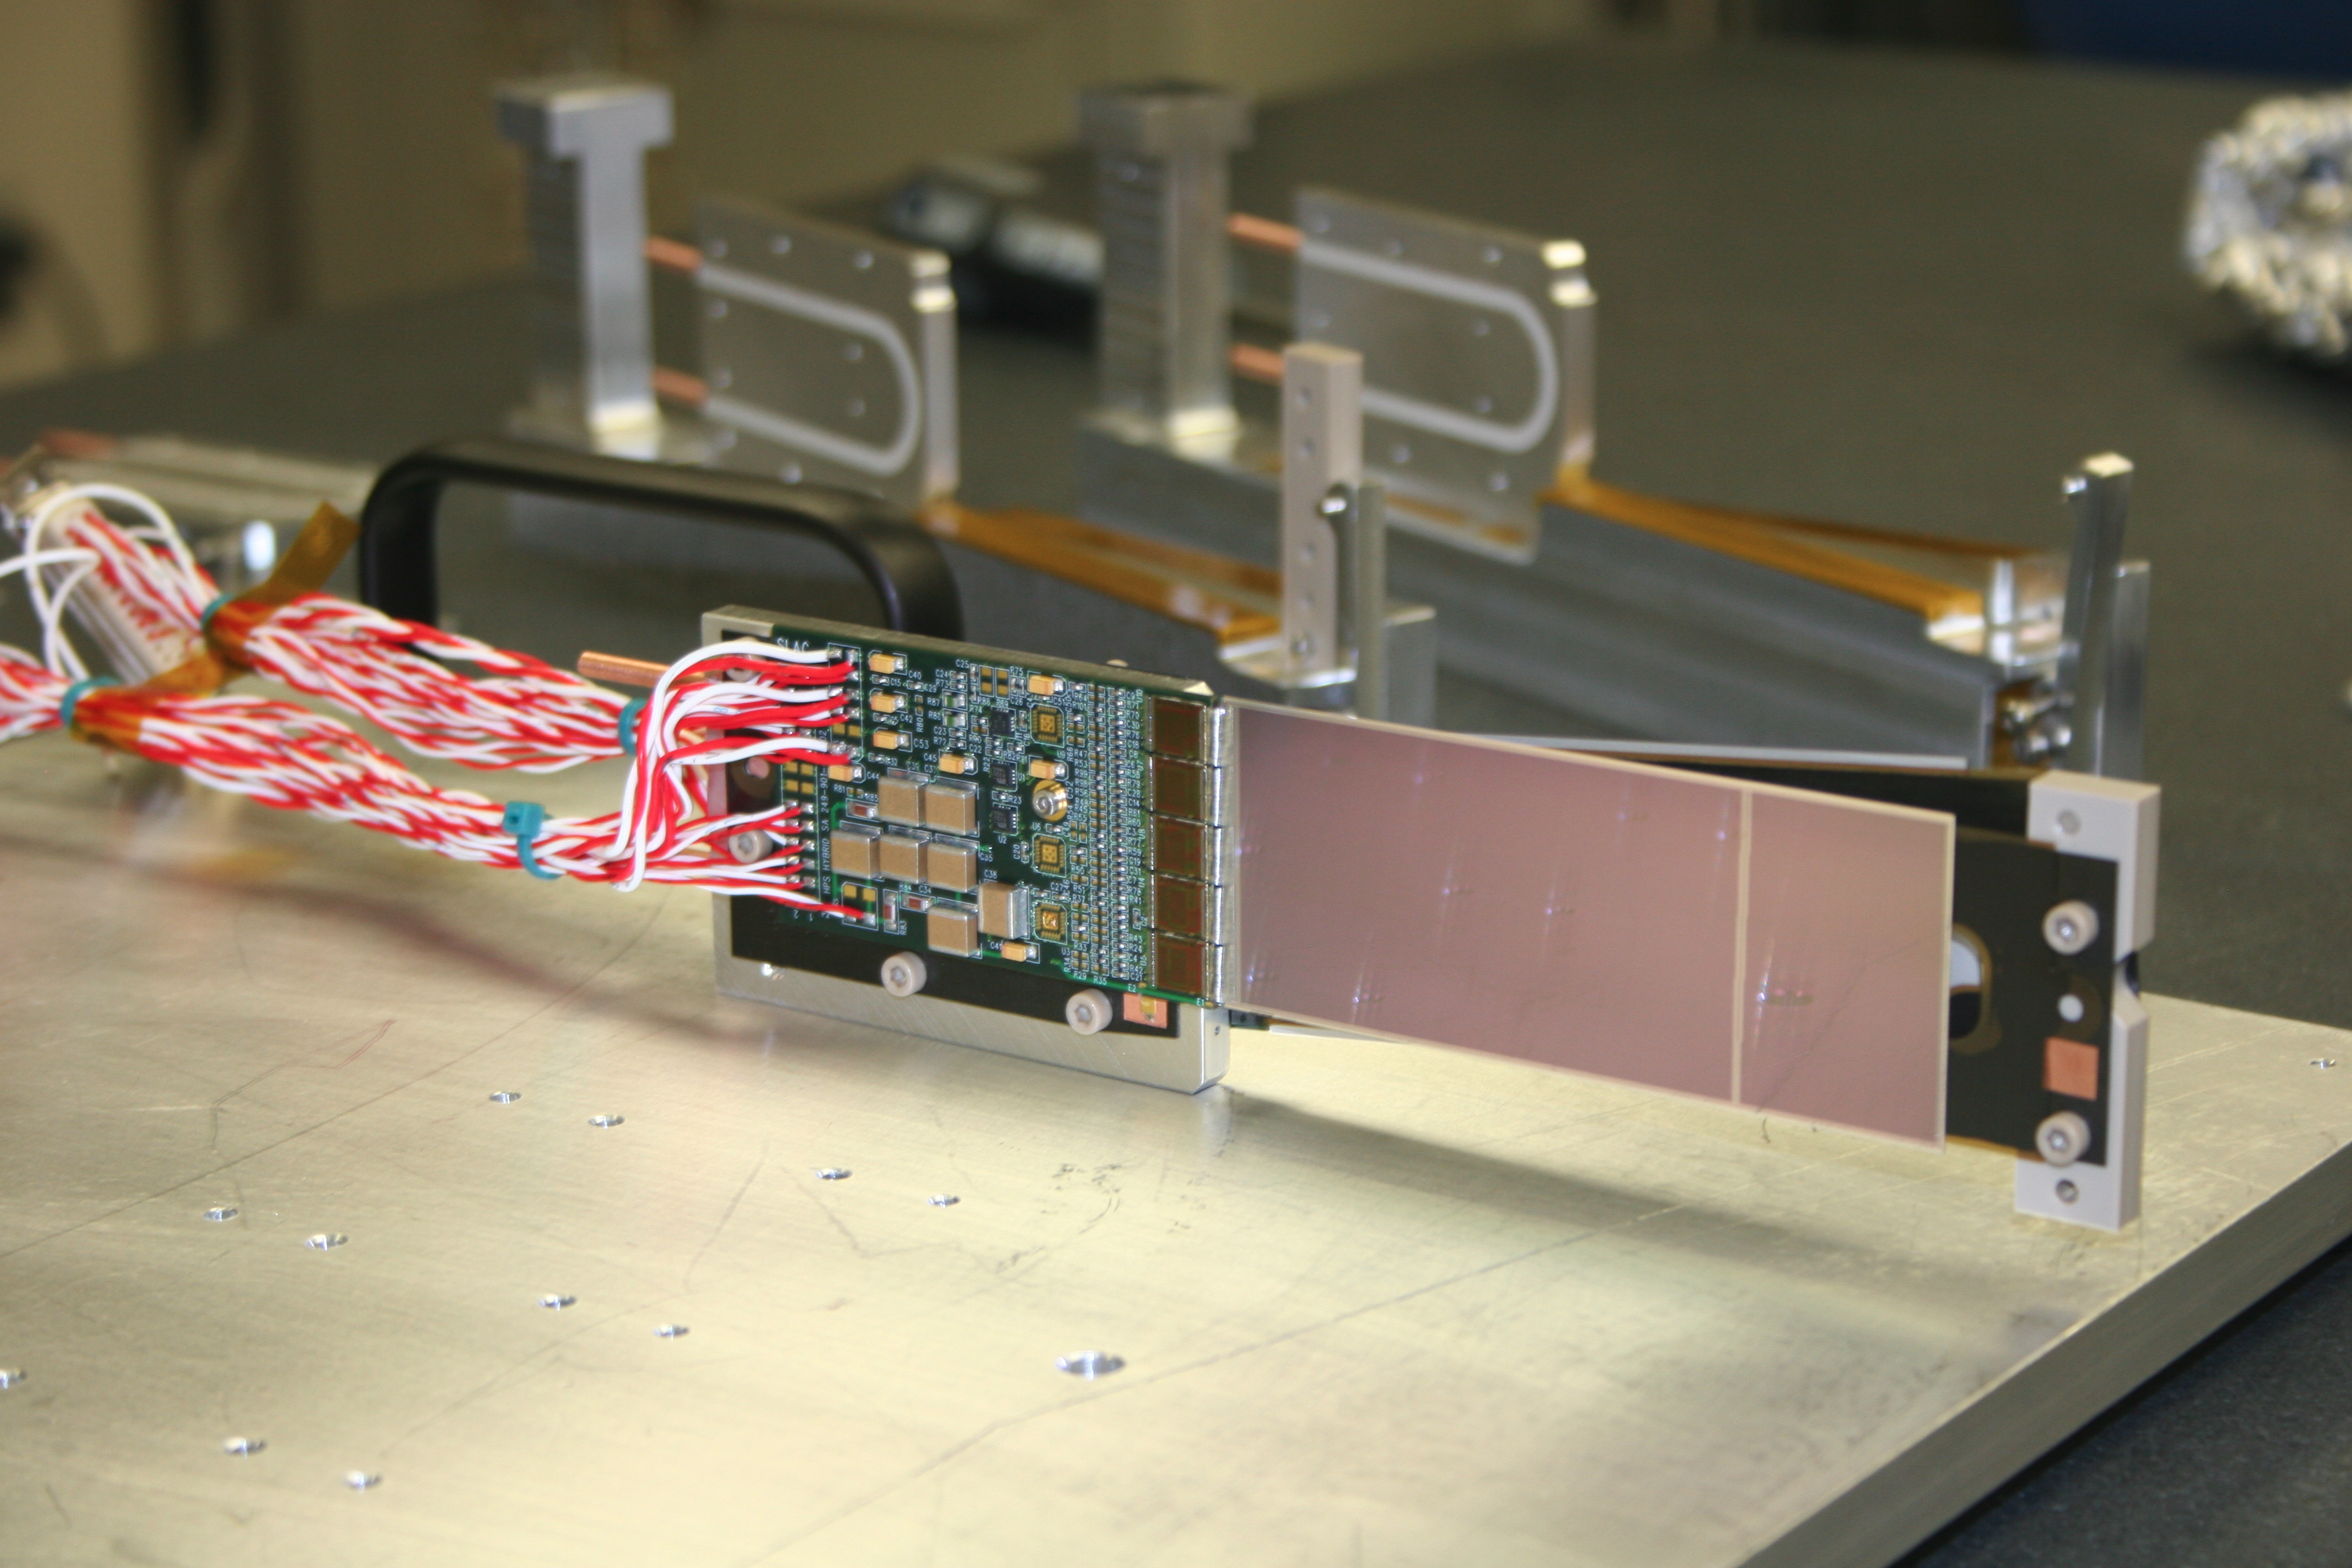
\includegraphics[width=0.5\textwidth]{figs/detector/module.png}
    \caption{A single SVT module which comprises of two silicon microstrip sensors which are axial (front) and stereo (back) to the beam plane. Each sensor is supported by a carbon fiber support structure can be seen protruding from the right of the axial sensor.}
    \label{fig:svtmodule}
\end{figure}

Each sensor is part of a base unit referred to as a ``half-module" and is comprised of a single or double sensor, carbon fiber support structure, and hybrid readout circuit boards. The first three layers 1-3 are composed of a single sensor and hybrid while the last three layers 4-6, since they are double wide, are composed of double sensors and hybrids. Each of these half-modules can be used as the axial or stereo components of the detector.

The carbon fiber, in addition to support for the sensor, acts as ground plane for the half-module while a layer of Kapton insulation isolates the carbon fiber from the back of the sensor which is at high voltage. The Kapton and carbon fiber are kept as thin as possible, much thinner than the silicon sensors, to avoid adding additional unnecessary material that increases multiple scattering in the tracker.\footnote{A window was machined into the carbon fiber support such that the material in the middle of the sensor, where most of the physics of interest is expected, is further minimized.}

The hybrid circuit boards house the APV25 readout chips, five per half module, and provides a connection of the sensor to the rest of the DAQ. The APV25 power, control lines, and output channels are wirebonded to the hybrid while the input channels are wirebonded directly to the sensor. The hybrid contains temperature sensors and carries filter capacitors for the sensor bias.

Two of these half-modules are paired to create a module with one axial and one stereo half-module. The axial half-modules are parallel to the beam plane and the stereo half-modules are rotated at a small angle and dips into the beam plane on the positron side (beam left, the side opposite to where beam background is bent). These modules are mounted on aluminum support modules which hold the half-modules from both sides and, in addition to mechanical support, these supports also pull heat generated by the hybrids. The half-modules and the support undergo thermal contraction at different rates, thus the module support applies a constant tension from a spring pivot in order to keep the half-modules flat at operating temperature ($\sim 0^{\circ}$ C). A picture of a complete module is shown in Fig. \ref{fig:svtmodule}.

Three of these modules are mounted on an aluminum support structure called a ``U-channel". The SVT contains a total of four of these U-channels for each top and bottom of L1-3 and L4-6 (which are larger). Each U-channel is supported by kinematic mounts which guarantee reliable and repeatable positioning when the U-channels are installed and re-installed. The L1-3 U-channels rest on two downstream kinematic mounts, which act as a hinge, and is supported at the upstream end by motion levers which guide the L1-3 U-channels towards and away from beam. Finally, the L1-3 modules house scan wires as close to the target position as possible to measure the beam position and profile relative to the SVT to assess beam quality. Each U-channel has two wires - one parallel to the beam plane and one rotated at a slight angle - in order to obtain 2D position information. A picture of a L1-3 U-channel is shown in Fig. \ref{fig:uchannel}.

\begin{figure}
    \centering
    \includegraphics[width=0.5\textwidth]{figs/detector/U1-3.png}
    \caption{Layers 1 - 3 modules of the SVT (from left to right) are place in one of the U-channels. Copper cooling lines and electrical lines can be seen. The wire frames and scan wires can also be seen on the left.}
    \label{fig:uchannel}
\end{figure}

The SVT underwent a mechanical survey before installation using a coordinate-measuring machine which utilized both optical and touch probe measurements to locate 3D target points. The survey ensures the SVT was assembled as designed and allows adjustment for the adjustable components if necessary, and it provides an initial alignment for track reconstruction whose quality depends strongly on precise knowledge of the sensor positions and orientations. This is sufficient for initial knowledge, but the sensor is later aligned using the data as described in Sec. \ref{sec:alignment}. Lastly, the survey provides a measurement of the edge of the L1 axial sensor relative to the wire on the U-channel to ensure that the sensor edge is placed at 500 $\mu$m from the beam plane. A picture of the SVT installed in the SVT vacuum box is shown in Fig. \ref{fig:svtvaccum}.

\begin{figure}
    \centering
    \includegraphics[width=0.95\textwidth]{figs/detector/vacuumbox.png}
    \caption{A picture inside the SVT vacuum chamber with everything installed except for the target. The frontend boards (FEBs) and FEB cooling plate are on the left. The SVT cooling lines protrude outward in the picture. The first layer of the SVT can be seen in the back behind the wire frames. The SVT is in its closed position and the beam must go through the 1 mm gap between the top and bottom sensors.}
    \label{fig:svtvaccum}
\end{figure}

%A coordinate-measuring machine uses both optical and touch probe measurements to locate 3D target points. The touch probe has higher precision in general so it is used whenever possible, though the optical measurement must be made on the silicon sensors themselves. Several different measures are made. First, individual sensors are measured with respect to . Finally, the fully assembled U-channels are measured as a cross-check with the other measurements...

\clearpage

\subsection{SVT Data Acquisition, Power, and Services}\label{sec:svt_daq}

\begin{figure}
    \centering
    \includegraphics[width=0.5\textwidth]{figs/detector/svt-daq-schematic.png}
    \caption{A schematic of the SVT DAQ system described in Sec. \ref{sec:svt_daq}.}
    \label{fig:svtdaq}
\end{figure}

HPS must have a method to pass power and data to the detector given the constraints of the detector design as described previously. In addition, the nearest rack that can contain the data acquisition (DAQ) and power supplies is located about 20 m from where HPS is installed thus requiring the analog signals from the APV25 readout chips to be converted to optical digitized signals. As a result, the signal digitization and low-voltage regulation is performed inside the vacuum on front end boards (FEBs) located on a cooling plate alongside the SVT. And because the SVT and front end boards (FEBs) are in vacuum, all power and DAQ must pass through a pair of 8-inch vacuum flanges upstream of the dipole magnet, thus requiring the reduction of the number of signals.

Each of the 10 FEBs can service either a pair of L1-3 modules or a single L4-6 modules totalling four hybrids which is connected by a single bundle of impedance-controlled twisted pair magnet wire (which reduces crosstalk and electromagnetic interference between the lines). This carries the analog APV25 output signals, digital controls, trigger signals, low-voltage power, and high-voltage sensor bias. The data and control signals are carried by a mini-SAS cable on a high-speed data link. The FEBs digitize the output signals from 20 APV25 chips (4 hybrids $\times$ 5 APV25 chips). A preamplifier on the APV25 converts a differential current signal to voltage and is digitized to a value between 0 and 16384 by an AD9252 14-bit analog to digital converter (ADC) which samples the signal at 41.667 MHz.\footnote{The 14-bit samples for each of the 23040 APV25 channels is too much data to store. The DAQ requires a readout threshold of three out of six samples above a threshold (three times the channel noise above the mean) that is predetermined from offline calibration.} Each FEB contains a Xilinx Artix-7 FPGA that sends the ADC data upstream to multi-gigabit receivers and controls and monitors the hybrid state and configuration.

%FEBs also distribute low-voltage power to the hybrids by supplying a single voltage by splitting into four independent voltages and using a combination of switching and linear voltage regulators. Improves noise performance, reduces number of voltages that must be passed through vacuum chamber. High-voltage is also passed, but directly.

The digitized data, low-voltage power, and high-voltage bias from the FEBs is transferred to electronic boards on the penetration of the vacuum flange (called ``flange boards'') through mini SAS cable for data and twisted pair cables for power and bias.\footnote{The flange boards are custom-made since the number of required connections is too high for conventional vacuum feedthroughs.} There are two flange boards on the beam right side - one for high voltage and the other for low voltage. The four flange boards located on the beam left side convert the digitized signal to optical using fiber transceivers so the signal can be transferred a large distance to the general-purpose Reconfigurable Cluster Elements (RCE) platform. The RCE platform was developed at SLAC and is housed in a standard Advanced Telecommunications Computing Architecture (ATCA) crate. The data from the FEBs is distributed on a Cluster on board (COB) between two ATCA blades housed inside the crate. Each COB contains 8 RCE processing nodes which use Xilinx Zynq-7000 series FGPAs to apply data reduction to signals from the flange boards and build events.

Each COB houses several generic hardware daughterboards common to RCE platforms including four Data Processing Modules (DPM) and one Data Transport Module (DTM). The DPMs process and reduce data at high speed while the DTM is responsible for timing and trigger distribution. The only HPS-specfic hardware on the COB is the Rear Transition Module (RTM) which interfaces the optical fibers from the signal flange boards to the COB. The SVT DAQ utilizes a total of two COBS and two RTMs. In addition to the core of the DAQ, the rack also contains the low and high voltage Wiener MPOD power supplies which are commonly used for a variety of JLab experiments. A schematic of the SVT DAQ system is shown in Fig. \ref{fig:svtdaq}.

The SVT services - motion, cooling, and power - are supplied from outside the vacuum through several flanges located upstream of the vacuum chamber. The SVT is cooled through two independent cooling loops - one for the silicon sensors and the other for the FEBs. The silicon sensors must be kept below 0$^{\circ}$ C in order to avoid further radiation damage due to higher temperature (called reverse annealing). They are cooled through a hydrofluoroether compound circulating through copper lines embedded into the U-channels where the top and bottom are split and L1-L3 and L4-L6 are connected in series. The specialized fluid is necessary since its low viscosity maintains high flow rates at low temperatures.

%The FEBs only need to be kept at around room temperature while dissipating only the heat the produced from operating the FEBs themselves. 
Only the heat produced from operating the FEBs themselves needs to be dissipated. Thus, distilled water is sufficient as a cooling fluid and is circulated through copper lines embedded in the FEB cooling plate. The FEBs themselves are cooled through direct thermal contact with the cooling plate. A picture of the FEBs on the cooling plate is shown in Fig. \ref{fig:FEBcooling}.

\begin{figure}
    \centering
    \includegraphics[width=0.5\textwidth]{figs/detector/FEBcooling.png}
    \caption{The FEB cooling plate complete with 10 FEBs fastened to the front and back of the plate.}
    \label{fig:FEBcooling}
\end{figure}

In addition to cooling components, there are three linear shift stepper motors that provide independent motion control of the top and bottom U-channels as well as the target frame. The motors are powered and controlled by a Newport XPS controller. All three motors have both a hardware and software safety stop, while the two motors that control the U-channel linear motion also include a precision limit switch to ensure the SVT is not accidentally driven into the beam.

\clearpage

\section{Electromagnetic Calorimeter and Trigger}\label{sec:ecal}

\begin{figure}
    \centering
    \includegraphics[width=0.85\textwidth]{figs/detector/ecal.png}
    \caption{A rendering of the beam's eye view of the HPS Ecal. Each segment is one of the 442 lead tungstate crystals and the Ecal is split in half to avoid radiation damage from the most intense parts of the beam.}
    \label{fig:ecal}
\end{figure}

The electromagnetic calorimeter (ECal) is an array of 442 lead tungstate scintillating crystals (PbWO$_4$) and is used primarily for precision timing and triggering \cite{Balossino_2017}. The crystals are reused from the CLAS Inner Calorimeter (IC). The crystals have front faces of size 1.3 $\times$ 1.3 cm$^2$, are 16 cm long, and are tapered such that the back faces have dimensions 1.6 $\times$ 1.6 cm$^2$ for acceptance purposes. The Ecal itself is split into top and bottom halves much like the SVT to avoid the most intense parts of the beam plane. Each half contains 5 rows of 46 crystals with the exception of the removal of 9 crystals in the innermost row to avoid large occupancy from beam background. This is referred to as the Ecal hole or electron gap. The innermost rows are positioned 2 cm from the beam plane to maintain the 15 mrad design opening angle. The face of the Ecal is positioned 139.3 cm from the target position. Scintillation light from each crystal is detected by an avalanche photodiode (APD) on the back face of the crystal (specifically, a Hamamatsu S8664-1010 APD). One blue and one red LED are positioned on the front face of each crystal and are used for monitoring purposes (specifically radiation damage and stability of readout gain). Since the scintillator response is temperature-dependent, the Ecal is surrounded by a thermal enclosure.

The primary purpose of the Ecal is to trigger the experiment. Jefferson Laboratory has developed general-purpose readout boards called the FADC250 digitizer boards, or simply FADC. APD signals are amplified by a preamplifier that outputs signals through a motherboard. Each FADC board has 16 input channels and are continuously digitized at 250 MHz to a 12-bit precision which are then stored in 8 $\mu$s deep pipelines to await being readout if a trigger signal is received. There are several readout modes available, but HPS utilizes the readout mode that outputs a window of 100 samples that allows pulse fitting with optimal time resolution.

\begin{figure}
    \centering
    \includegraphics[width=0.85\textwidth]{figs/detector/ecal_crystal.png}
    \caption{A schematic of a PbWO$_4$ crystal in the Ecal.}
    \label{fig:ecalcrystal}
\end{figure}

The FADC boards are located in VXS crates also developed by Jefferson Laboratory as a general-purpose trigger framework. An algorithm that continuously looks for threshold crossings and integrates the digitized signal from the FADC within a fixed window converts the integration to an energy from previously calibrated values from cosmic rays. This gives a crystal position, energy, and time of the threshold crossing which are then passed to the Global Trigger Processor (GTP) every 32 ns. Each Ecal half has a GTP board which clusters hits by looking at a 3 $\times$ 3 block around a center crystal with at least 50 MeV and the surrounding hits within 16 ns of the center hit. This defines a cluster with a center crystal, hit time, number of hits, and total energy. Each GTP reports these clusters to the Single Subsystem Processor (SSP) board.

The SSP uses these clusters to make a decision on the Trigger. For the 2016 Engineering Run, there were a total of 5 triggers utilized. The first is a ``pulser'' trigger which fires at a fixed rate of 100 kHz. Next, there are two triggers that fire on single clusters that are called ``singles1'' and its corresponding trigger which has looser requirements ``singles0''. Finally, there are two triggers that fire on a pair of top-bottom clusters (at least one cluster in each GTP). These are called ``pairs1'' and ``pairs0'' triggers, where pairs0 is the looser version of pairs1. The pairs1 is our nominal trigger that is used for the physics analysis. In order to prevent the other triggers from triggering at a rate higher than the DAQ can handle, the singles triggers and the pairs0 trigger are prescaled such that one trigger in $2^n$ triggers are accepted where n is in the range of 10 to 13.

Once the SSP makes a trigger decision, if a cluster or pair of clusters meets the requirements above a trigger is sent to the Trigger Supervisor board (TS) and distributes the trigger to the Trigger Interface (TI) boards. The TS can reject the trigger if a subsystem is not ready to accept a trigger or the trigger follows too closely to another trigger.

The livetime of the DAQ, that is the fraction of time the DAQ is willing to receive triggers, must be understood in order to properly normalize the data. One way to measure the livetime is to use the pulser trigger. Since the pulser trigger fires at a constant rate, the ratio of the number of pulser triggers recorded to the number of pulser triggers that should have been recorded based on the 100 Hz rate is a direct measurement of the livetime. Another way to measure the livetime is to combine the measurement of integrated charge from the Faraday cup as described in Sec. \ref{sec:beamline} with a measurement of the integrated charge with the DAQ live. This is called the ``gated Faraday cup scaler'', and the ratio of this scalar to the total integrated charge is the DAQ livetime.

\begin{figure}
    \centering
    \includegraphics[width=0.85\textwidth]{figs/detector/ecal_trigger.png}
    \caption{A schematic of the trigger for the Ecal. Top and bottom halves of the Ecal are each are readout by FADC readout boards, and then sent to the SSP where a trigger decision is made.}
    \label{fig:ecaltrigger}
\end{figure}

The HPS physics trigger is designed to maximize efficiency for $A's$, or more generally $\epem$ pairs near the beam energy, while sufficiently suppressing backgrounds to avoid overwhelming the DAQ systems. The most significant one-cluster background is electrons elastically-scattered in the target. Thus a trigger requiring at least two clusters will eliminate a large fraction of these. The largest source of two-cluster backgrounds is wide-angle bremsstralung (WABs) in coincidence with a beam electron elastically scattered in the target. These can be eliminated by first requiring top and bottom coincident clusters as well as further timing and energy cuts.

The time coincidence between top and bottom clusters is required to be within 12 ns and is corrected for time walk. In addition to timing requirements, there is a coplanarity requirement that requires two clusters on opposite sides of the beam axis. It is intended to select only $\epem$ coincident pairs which are expected on average to be symmetric about the beam axis. The azimuthal angle $\phi$ relative to the beam axis of the top and bottom cluster is required to be within $\pm 30^{\circ}$ of $180^{\circ}$.

Furthermore, the trigger requires some basic energy requirements. First, a maximum energy sum requirement eliminates a large fraction of coincident beam scattered electrons. For the minimum energy requirements, it is important to note that there are substantial energy losses from a variety of sources in the Ecal such as the absorption of energy by the vacuum flange, gaps between crystals, or the back of the Ecal. This is accounted for in the reconstruction by detailed MC studies, but is not accounted for in the trigger. In addition, particles can hit the innermost row of the Ecal and lose energy where much of the shower is lost in the beam gap. This is especially important since a large fraction of signal, particularly at lower mass due to the smaller opening angle, occurs at the beam edge of the calorimeter. For this reason, there are only loose requirements on the minimum energy on individual clusters and minimum energy sum that are below the truth energy threshold of what one would expect from an $A'$. Simulation shows that the looser energy requirement allows fully efficient triggering.

Finally, it is expected that the lower energy decay particles from $\aprime$s will have be further from the beam axis due to increased bending of the lower momentum particle from the magnetic field. The energy-distance cut rejects particles that are both low energy and close to the beam axis. This cut has the effect of first rejecting wide-angle bremsstrahlung which is a photon that is typically lower energy and closer to the beam axis and second, rejecting beam electrons that scrape the Ecal edge where most energy is lost. The cut is based on the cluster energy $E_{low}$ and the cluster distance from the beam axis $r_{low}$ and is expressed as $E_{low} + (5.5$ \ MeV / mm$) \ r_{low} > 0.7$ \ GeV.

The pairs1 trigger requirements - including the timing, cluster energy, cluster size, energy sum, cluster energy difference, coplanarity, and energy-distance requirements - are summarized in Table \ref{tab:trigger}.


\begin{table}[!hb] 
    \centering
    \begin{tabular}{lc}
        \toprule
        \textbf{Trigger Description} & \textbf{Value} \\
        \midrule
        \midrule
            Time Difference & $|t_{top} - t_{bot}| \leq 12$ ns \\
            Cluster Energy & $0.15 < E < 1.4$ \ GeV  \\
            Cluster Size & $N_{hits} \ge 1$ \\
            Energy Sum & $0.6 < E_{top} + E_{bot}< 2.0$ \ GeV \\
            Energy Difference & $|E_{top} - E_{bot}| < 1.1$ \ GeV \\
            Coplanarity & $|\phi_{top} - \phi_{bot} - 180^{\circ}| < \ 35^{\circ}$ \\
            Energy-Distance & $E_{low} + (5.5$ \ MeV / mm$) \ r_{low} > 0.7$ \ GeV \\
        \bottomrule
    \end{tabular}
    \caption{Summary of the pairs1 Trigger Selection from the 2016 Engineering Run.}
    \label{tab:trigger}
\end{table}

\clearpage

\section{Datasets}\label{sec:datasets}

\begin{figure}
    \centering
    \includegraphics[width=0.75\textwidth]{figs/detector/2015_data.png}
    \includegraphics[width=0.75\textwidth]{figs/detector/2016_data.png}
    \caption{A summary for the integrated charge over time for the Top: 2015 Engineering Run and Bottom: 2016 Engineering Run.}
    \label{fig:datasets}
\end{figure}

To date, HPS has three data taking runs - an engineering run in 2015, an engineering run in 2016, and a physics run in 2019. The 2015 engineering run was taken with a beam energy of 1.056 GeV and beam current of 50 nA incident on a 4 $\mu$m target. The total luminosity taken over opportunistic nights and weekends amount to 1166 nb$^{-1}$ which corresponds to 1.7 PAC days. A broken cryogenic helium liquifier (CHL) shortly before the run began resulted in the operation of only a single CEBAF linac for this run (as opposed to the usual two linacs). This gave HPS a unique opportunity to run at this beam energy equivalent to half a pass which would have otherwise been unavailable.

The 2016 Engineering Run was taken with a beam energy of 2.3 GeV and beam current of 200 nA incident on a 8 $\mu$m target. The total luminosity taken over weekends amount to 10753 nb$^{-1}$ which corresponds to 5.4 PAC days. Much of the analysis is performed on a blinded $\sim 10$\% sample (1101 $nb^{-1}$) before the final results over the whole dataset are produced. The data for the 2016 Engineering Run was collected by running on weekends over the span of several months.

A summary of the accumulated luminosity over time for the 2015 and 2016 Engineering Runs is shown in  Fig. \ref{fig:datasets}. The focus of this thesis is the displaced vertex analysis from the 2016 engineering run. The 2019 Physics Run was undertaken with an upgraded detector, described in Sec. \ref{chap:upgrades}.

%to 0.4671 mC????
\chapter{Event Reconstruction \& Selection}\label{chap:reconstruction}

Reconstruction is the process in a given event of building actual physics processes, such as an $\aprime$ decay, from the raw hits of the detector channels readout by the trigger. The HPS event reconstruction is based on the lcsim software toolkit \cite{Graf_2011} and uses both reconstructed energy clusters from the Ecal and tracks from the SVT, which are done independently until Ecal clusters and tracks are matched by extrapolating the track state at the last layer of the SVT to a cluster in the Ecal for particle identification. These objects, mainly $e^+e^-$ pairs or $e^-e^-$ pairs, are used to reconstruct vertices used for the physics analysis. The multiple stages of the HPS reconstruction - SVT hit reconstruction, tracking, vertexing, and Ecal clusters - are discussed in the following sections.

\section{HPS Coordinate Systems}\label{sec:coordinates}

\begin{table}[!hb] 
\centering
\begin{tabular}{lccc}
   \toprule    
    Coordinate System & $x$ & $y$ & $z$ \\
    \midrule
     JLab Coordinates & Beam left & Vertical & Beam direction \\
     Detector/HPS Coordinates & Beam left rot. -30.5 mrad & Vertical & Beam direction rot. -30.5 mrad \\
     Tracking/lcsim Coordinates & Beam direction & Beam left & Vertical \\
     \bottomrule
\end{tabular}
\caption{Basis for several different coordinate systems used in the HPS reconstruction and analysis.}
\label{table:coordinates}
\end{table}

\begin{figure}[t]
    \centering
    \includegraphics[width=.5\textwidth]{figs/recon/lcsim_1.png}
    \includegraphics[width=.4\textwidth]{figs/recon/lcsim_2.png}
    \caption{A schematic of the linear collider tracking parameters \cite{Kraemer:81214}. %http://flc.desy.de/lcnotes/notes/localfsExplorer_read?currentPath=/afs/desy.de/group/flc/lcnotes/LC-DET-2006-004.pdf
    }
    \label{fig:track_params}
\end{figure}

There are three coordinate systems utilized in the HPS reconstruction process - the global coordinates (JLab coordinates), the HPS coordinate system (detector coordinates), and tracking coordinates (lcsim coordinates). Each coordinate system is used in a different part of the reconstruction process since each has simplifying features. First, the JLab coordinate system is defined globally by the Hall B beamline where the the $x$-axis points beam left in the bend plane, the $y$-axis points vertically upwards, and the $z$-axis points along the direction of the beam. The origin is set at the intersection of the nominal beam and nominal target position. Due to the asymmetry of HPS with respect to the chicane, where the beam is bent due to the first dipole magnet in the chicane by 30.5 mrad about the $y$-axis in the $-x$-direction, the HPS $z$-axis and $x$-axis are also rotated by 30.5 mrad. Since the beam travels in the $+z$-direction in HPS coordinates at the target, this is the natural reference frame for reconstructed particles and, unless otherwise stated, the physics analysis including positions and momenta will utilize this frame.

The entire HPS SVT lies within a roughly uniform vertical magnetic field, thus a charged particle trajectory will form a helix. Unfortunately, the coordinate systems for track reconstruction and analysis on HPS are different. HPS utilizes perigee parametrization of tracks that fixes a magnetic field along the $z$-axis (which is the $y$-axis in HPS coordinates). The tracking coordinates are oriented approximately such that the $x$-axis points along the direction of the beam, the $y$-axis points beam left, and the $z$-axis points vertically upwards. In addition, each track is defined by 5 track parameters - $\Omega$, $d0$, $z0$, $tan \lambda$, and $\phi$ - and are briefly described below and shown in Fig. \ref{fig:track_params} \cite{Kraemer:81214}.

\begin{enumerate}
  \item $\Omega$ is the signed curvature of the track (i.e. the inverse of the radius $C=-q/R$).
  \item $d0$ is the signed impact parameter in the $xy$ tracking plane. In the HPS detector frame, this translates to the impact parameter along the $x$ (horizontal) direction.
  \item $z0$ is the tracking $z$ position at the point of closest approach to the reference point. This is the key tracking parameter for the isolation cut. In the HPS detector frame, this approximately corresponds to the impact parameter in the $y$ (vertical) direction.
  \item tan$\lambda$ is the slope of the straight line in the $sz$ tracking plane. In the HPS detector frame, this translates to the slope of the track $dy/dz$ in the $yz$ plane.
  \item $\phi$ is the azimuthal angle of the momentum of the particle at point of closest approach to the reference point.
\end{enumerate}

Due to multiple scattering in the silicon sensors, each segment of the track between scattering planes is described by a separate helix, called a track state. Thus, each track segment will have its unique 5 track parameters as well as a unique 5 $\times$ 5 covariance matrix of these track parameters, and a track will have 11 or 13 track states depending on the number of hits on track. This process is described in Sec \ref{sec:tracking}. The last importnat tracking parameter is the path length of the helix, denoted as $s$, which is useful for parametrization of the helix.

\section{Ecal Reconstruction}\label{sec:ecal_recon}

Electromagnetic particles that are incident on the Ecal and shower within the Ecal deposit energy in several crystals which can then be clustered together to give both the total energy deposited and an estimate of the hit position on the front face of the Ecal. The Ecal reconstruction is the process of building particle clusters from the waveforms readout in single crystals of the Ecal for a given event. Ecal crystals that are readout store 100 samples in 4 ns intervals relative to the trigger time. The pulse shape is fit with a three-pole function 

\begin{equation}
    F_{3pole}(t) = \frac{t^2}{2 \tau^3}e^{-\frac{t}{\tau}}
    \label{eqn:ecal_recon}
\end{equation}

The time constant $\tau$ is calibrated offline for each channel and is typically $\sim 2.4$ ns. From this function, the pedestal, time of the pulse, and amplitude are fit in offline reconstruction and pileup is ignored. From the amplitude, the pulse is converted to energy by two types of channel calibrations - cosmic rays and elastic scatters in the target \cite{ecalpulse}. Cosmic rays, which pass downward through the Ecal and deposit a calculable amount of energy in the crystals, are used for a preliminary Ecal calibration before data taking. After data taking, cluster energy is calibrated with electrons elastically scattered by the target, which are very near the beam energy, and the gain constants for every crystal are adjusted until the energies match what is observed in MC. Cosmic ray MIPs and elastically scattered electrons sample the full range of interest in energy.

%Cosmic rays are calibrated before data taking with the beam off through the detection of minimum ionizing particles (MIPs), which have a known rate of energy loss, passing downwards through the Ecal.

%Cosmic rays, which pass downward through the ECal and deposit a calculable amount of energy in the crystals, are used for a preliminary Ecal calibration.

In order to form clusters in the Ecal, individual hits are grouped together using a clustering algorithm adapted from the CLAS Inner Calorimeter \cite{ASRYAN2020163425}. A crystal which has the most energy in a local group of hits becomes the seed for a cluster, and the algorithm looks for hits in neighboring crystals which are within 8 ns of the seed to build the cluster. Since higher energy hits have better timing resolution, the seed hit time is defined as the time of the cluster. %The seed hit time is used as the time of the cluster with larger energy since higher energy hits have better timing resolution. %Hits with a local energy maxima are seeded for clusters, and then the algorithm searches for neighboring crystals with seeds or a hit on a cluster within 8 ns of the seed. The seed hit time is used as the time of the cluster with larger energy since higher energy hits have better timing resolution. 

The energy of the cluster is initially the sum of the individual hit energies. However, this energy does not account for parts of the electromagnetic showers that are lost on the Ecal edges or absorbed in the vacuum flanges. In addition, particles generally enter an Ecal crystal at an angle off axis from crystal axis and electromagnetic showers deposit energies at all Ecal depths resulting in the fact that maximum energy deposition may not occur in the same crystal as the crystal whose front face the particle has traversed. As a result, energy corrections are based on detailed MC studies and the energy is corrected as a function of particle type (photon, electron, or positron), energy, and angle, where the particle type must be determined by track-cluster matching later in the reconstruction described in Sec. \ref{sec:trackcluster}. In addition, the position of the cluster is initially determined by a logarithmically-weighted centroid. For the same reason as energy, the position must also be corrected and is done so in the same MC studies as energy \cite{ecalsim} \cite{ecalenergy}.

\clearpage

\section{SVT Reconstruction} \label{sec:svtrecon}

The SVT reconstruction is the process of building particle tracks from the collection of waveforms readout from all the single strips in the SVT which have been hit. These tracks are used to form electron and positron objects (tracks matched with Ecal clusters), which are then used to form vertices used in the final analysis.

\subsection{SVT Hit Reconstruction}
For each trigger, SVT channels where at least three of the six samples are above the readout threshold, that was determined by offline calibration before data taking in calibration runs (for reasons described in Sec. \ref{sec:svt_daq}), are readout. For each strip in the SVT that is readout, the APV25 reads out six samples at 24 ns intervals. The APV25 response is modeled as a four pole filter with three coincident poles (i.e. three of the poles with the same time constant). This gives the following transfer function with two time constants $\tau_1$ and $\tau_2$.

\begin{equation}
    \tilde{F}(\omega)=\frac{1}{(1+i \omega \tau_1)(1+i \omega \tau_2)^3}
    \label{equ:transfer}
\end{equation}

The inverse Fourier Transform of this transform function is the pulse shape given by

\begin{equation}
    F(t,\tau_1,\tau_2)=A \frac{\tau_1^2}{(\tau_1-\tau_2)^3} \left(  e^{-\frac{t-t_0}{\tau_1}}-\sum_{k=0}^2 \left( \frac{\tau_1-\tau_2}{\tau_1 \tau_2}(t-t_0) \right)^k \frac{e^{-\frac{t-t_0}{\tau_2}}}{k!} \right)
    \label{equ:sample_fits}
\end{equation}

The time constants are predetermined offline by fitting pulses in calibration runs and have typical values of $\tau_1 \approx 72$ ns and $\tau_2 \approx 12$ ns. $t_0$ is defined as the time the fit crosses 0 and is set as the time of the raw hit. $A$ is related to the amplitude of the pulse in ADC counts. Both of these quantities are determined by the fit in offline reconstruction and an example waveform and fit is shown in Fig. \ref{fig:6samples}.

The pulse is fit to a pileup algorithm where a fit to a single pulse is compared to a fit with a double pulse. If the single pulse fit has a $\chi^2$ probability less than 0.5, a refit with two pulses is attempted. If this produces an improved $\chi^2$ probability, the double pulse fit is accepted, else the single pulse fit is accepted. The time of the pulse is corrected after the fit for several effects including a run-dependent phase shift, trigger time, and time of flight. %The $t_0$ is corrected in reconstruction for several affects. First, $t_0$ is corrected by a run-dependent phase shift or offset time. Then $t_0$ corrected for the trigger time. Then trigger hitter and the time scale is subtracted (55). Then, subtract $t_0$. The $t_0$ is shifted sensor-by-sensor. Then time of flights corrects are applied based on sensor position. /textcolor{red}{I am very confused by all these time shifts - Matt S.}

\begin{figure}[t]
    \centering
    \includegraphics[width=.85\textwidth]{figs/recon/6samp.png}
    \caption{A plot of the digitized waveform that is output from the APV25 and is fit using Eq. \ref{equ:sample_fits}. The 6 samples used for the fit are in 24 ns intervals (between the red lines).
    }
    \label{fig:6samples}
\end{figure}

\clearpage

\subsection{SVT Cluster and 3D Hit Reconstruction}
After single strip hit reconstruction, the hits are clustered together with neighboring hits using the nearest neighbor RMS Clusterer algorithm. The algorithm uses the amplitudes in ADC counts (where it is not necessary to convert amplitude to energy deposition) and seeds hits whose amplitude are at least 4$\sigma$ above the noise of the channel, where $\sigma$ is the RMS of the noise of the channel. From there, it appends neighboring strips whose pulse times are within 8 ns of the seed strip and whose amplitudes are at least 3 RMS above the noise of the channel. In addition, each of the strips, whether seed or neighbor channel, must have a $\chi^2$ probability for the fit in Eq. \ref{equ:sample_fits} greater than $3.20 \times 10^{-6}$.  %($Q(4,20)$ where Q is the regularized gamma function). 
The position of the cluster is the amplitude-weighted centroid of the hits ($\sum x_i A_i/\sum A_i$). Typically, SVT clusters are composed of one or two strips hits in approximately equal proportion. Since time resolution is significantly degraded for hits with low energy deposition, the time of the SVT cluster is weighted by the square of the amplitude ($\sum t_i A_i^2/\sum A_i^2$).

The 1D strip clusters in each axial sensor in a given layer are then paired together with the corresponding stereo sensor in the same layer to form 3D hits. Only clusters within 12 ns of the trigger time and with at least an amplitude of 400 ADC counts are considered. As a reference, a minimum ionizing particle (MIP) will typically have an amplitude of $\sim 1200$ ADC counts. These clusters must cross physically in space from the perspective of the primary (with some tolerance) and be within a 16 ns coincidence of each other. A 3D hit is reconstructed at the intersection of the two strip clusters. Since this intersection depends on the track angle, the 3D hit position is recalculated every time the hit is used in a track fit to correct for parallax effects.

\clearpage

\subsection{Track Reconstruction} \label{sec:tracking}

The SeedTracker algorithm, which was developed for design studies with the SiD detector \cite{seedtracker}, is performed as a simple method of track finding for HPS. Seed tracks, that is tracks that result from SeedTracker, are found using several different track finding strategies. The tracking strategies are as follows.

\begin{enumerate}
  \item A track candidate is found using a particular three (of the six possible) 3D hits to form a helical track.
  \item This helix is extrapolated to a confirm layer and, if this confirm layer has a 3D hit consistent with the helix, this hit is appended to the helical trajectory. Else, the track candidate is discarded.
  \item Lastly this 4-hit track is extrapolated to the remaining two layers called the extend layers. The 3D hits in those layers that are consistent with the helix are appended. We require at least one of the extend layers to have a 3D hit consistent with the helix, thus requiring a minimum of five 3D hits on a track. If this extend requirement is not met, the track candidate is discarded.
\end{enumerate}

%Initially, a track candidate is found using three 3D hits which forms a helical track. This helix is extrapolated to a confirm layer and, if this confirm layer has a 3D hit consistent with the helix, this hit is appended to the helical trajectory. Else, the track candidate is discarded. Lastly this track is extrapolated to the remaining two layers called the extend layers, and appends the 3D hits in those layers that are consistent with the helix. We require at least one of the extend layers to have a 3D hit consistent with the helix, thus requiring a minimum of five hit tracks. If this extend requirement is not met, the track candidate is discarded. 

Four tracking strategies are used because any single strategy using this method will not find tracks that happen to miss a seed or confirm layer. The four tracking strategies used in the reconstruction are s-345 c-2 e-16, s-456 c-3 e-21, s-123 c-4 e-56, and s-123 c-5 e-46 where s, c, and e are abbreviations for seed, confirm, and extend, respectively. As an example, s-345 c-2 e-16 seeds track candidates using 3D hits on layers 3, 4, and 5. Then, this helical fit is extrapolated to layer 2, followed by layers 1 and 6. The seed tracks from 345 that successfully append a hit in layer 2 and either layer 1 or 6 are stored as a track candidate to be used for the remaining reconstruction.

In addition, there are several other requirements the track must pass. The RMS time of all the hits on the track must fall within 8 ns. The track must have a $\chi^2$ less than 100 (including an individual hit $\chi^2$ less than 10), a distance of closest approach $d0$ less than 15 mm, an impact parameter $z0$ of less than 15 mm, and a minimum transverse momentum of 100 MeV. 

The SeedTracker algorithm returns a helical track fit to 3D hits, but fails to take multiple scattering into account which results in an artificially worsened momentum resolution. In order to account for multiple scattering effects, the helical track fit is refit using the General Broken Lines (GBL) algorithm \cite{BLOBEL200614} \cite{Kleinwort_2012}. For HPS, the GBL algorithm treats each sensor plane in the SVT as a source of scattering and fits a track segment (defined by 5 parameters described in Sec. \ref{sec:coordinates} that define the track state) between each sensor plane and extrapolates a track segment on the first and last SVT sensor plane. For the reconstruction of the 2016 Engineering Run dataset, the GBL track is required to have a $\chi^2$ per degree of freedom less than 12. The GBL fit minimizes the hit residuals and scattering angles (called kinks) for each of these track segments and provides performance equivalent to a Kalman filter. However, the GBL implementation for HPS requires 3D hits from SeedTracker before inputting the track into the GBL algorithm. This 3D hit requirement results in some efficiency loss due to acceptance for particles that only traverse either the axial or stereo sensor in a given layer. In addition, there are further efficiency losses due to the inherent efficiency effects of individual sensors where an inefficiency in either the axial or stereo sensor will not form a 3D hit. For future track reconstruction for HPS, a Kalman filter that utilizes strip hits for pattern recognition instead of 3D hits will be used to regain this loss of efficiency.

A plot of the hit efficiency for each SVT layer separated by hemisphere and curvature is shown in Fig. \ref{fig:hitefflay}. Layer 1 has decreased hit efficiency due a larger occupancy than the rest of the detector, while layer 6 has decreased hit efficiency due to a large number of dead channels in that layer. Positrons also have a decreased layer 1 efficiency due to wide-angle bremsstrahlung conversions in layer 1 in which a positron track extrapolates to layer 1 but may not leave a hit. The methods of measuring hit efficiency as well as separating the measurement by channel will be described in more detail in Sec. \ref{sec:hiteff}.

\begin{figure}[t]
    \centering
    \includegraphics[width=.45\textwidth]{figs/recon/hitefflayele.png}
    \includegraphics[width=.45\textwidth]{figs/recon/hitefflaypos.png}
    \caption{The hit efficiency for each top/bottom layer of the SVT for Left: electrons and Right: positrons. The decrease in efficiency in layer 1 and layer 6 can be attributed to increased occupancy and a large number of dead channels, respectively. The difference between electrons and positrons in layer 1 hit efficiency is a result of WABs, where a conversion occurs in layer 1 and fails to produce a hit in both axial and stereo sensors, which is measured as a hit inefficiency.
    }
    \label{fig:hitefflay}
\end{figure}

\clearpage

\section{Track Cluster Matching} \label{sec:trackcluster}
Tracks are matched to Ecal clusters by extrapolating the track state of the final SVT hit to the face of the Ecal though a non-uniform magnetic field map, which accounts for the dipole magnet's fringe field, and comparing this extrapolated position to the Ecal cluster position. Matching a track to an Ecal cluster confirms the reality of the track since all particles of interest that produce a track should also form an Ecal cluster.\footnote{In reality, particles of interest (typically electrons) can produce tracks but extrapolate to the so-called ``Ecal hole'' which was cut out to reduce occupancy from elastically-scattered beam particles. These tracks can be recovered by implementing a positron-only trigger and relaxing the requirement of an electron track matched to an Ecal cluster. This is done in the upgraded detector for future running described in Sec. \ref{sec:L0}.} In addition, since the Ecal offers a better time estimate than tracking, the time coincidence of two Ecal clusters can be used to reduce the effects of accidentals.

The track is matched with the cluster with the minimum $n_{\sigma}$, where $\sigma$ is the error on the extrapolated track position from layer 6 of the SVT to the front face of the Ecal , provided that the match is less than 30$\sigma$. Subsequent analysis imposes a stricter requirement. An electron object is defined as a negatively curved GBL track that is matched to an Ecal cluster in the same detector volume. Similarly, a positron object is defined as a positively curved GBL track that is matched to an Ecal cluster in the same detector volume. The electron and positron objects are used as inputs to the vertex fitter. The remaining Ecal clusters that do not have an associated matching track are defined as photon objects. At this beam energy, some muons and pions are present, but the vast majority of charged particles are electrons and positrons. Thus, nearly all the energy deposition in the Ecal is a result of electrons, positrons, and photons.

To potentially further reduce accidentals, one might expect the ratio of the energy of the Ecal cluster to the momentum of the matched track ($E/p$) to have a mean at one with a small $\sigma$ corresponding to the energy and momentum resolutions. However, the particles near the edge of the Ecal, where much of the action occurs, typically only deposit a fraction of their energy into the Ecal crystals. Thus, $E/p$ is non-Gaussian with a mean below 1 and as a result, no restriction on $E/p$ is imposed.

\clearpage

\section{Vertexing}

\begin{table}[t] 
    \centering
    \begin{tabular}{lr}
        \toprule
        \textbf{Cut Description} & \textbf{Requirement} \\
        \midrule
        Cluster Time Difference & $|t_{e^+ Cluster}-t_{e^- Cluster}|<2.5$ ns\\
        $e^{+}$ Track-Cluster Time Difference & $|t_{e^+ Track}-t_{e^+ Cluster} - 55| < 10$ ns\\
        $e^{-}$ Track-Cluster Time Difference & $|t_{e^- Track}-t_{e^- Cluster} - 55| < 10$ ns\\
        Ecal clusters in opposite volumes 
        	& $y_{\posi \mathrm{ Cluster}} \times y_{\ele \mathrm{ Cluster}} < 0$ \\
        Loose track-cluster match & $\chi^2 < 15$  \\
        Beam electron cut & $p(e^{-}) < 2.15$ GeV \\
        Track Quality & $\chi^2/dof < 12$ \\
        Maximum Vertex Momentum & $V_{0p} < 2.8$ GeV \\ 
        \bottomrule
    \end{tabular}
    \caption{Requirements applied to $V_{0}$ particles during the 
    		 reconstruction stage for data (i.e. preprocessing selection).}
    \label{tab:mouse_data}
\end{table}

\begin{table}[t] 
    \centering
    \begin{tabular}{lr}
        \toprule
        \textbf{Cut Description} & \textbf{Requirement} \\
        \midrule
        Cluster Time Difference & $|t_{e^+ Cluster}-t_{e^- Cluster}|<5$ ns\\
        Track-Cluster Time Difference & $|t_{e^+ Track}-t_{e^+ Cluster} - 43| < 10$ ns\\
        Track-Cluster Time Difference & $|t_{e^- Track}-t_{e^- Cluster} - 43| < 10$ ns\\
        Ecal clusters in opposite volumes 
        	& $y_{\posi \mathrm{ Cluster}} \times y_{\ele \mathrm{ Cluster}} < 0$ \\
        Loose track-cluster match & $\chi^2 < 15$  \\
        Beam electron cut & $p(e^{-}) < 2.15$ GeV \\
        Track Quality & $\chi^2/dof < 6$ \\
        Maximum Vertex Momentum & $V_{0p} < 2.8$ GeV \\ 
        \bottomrule
    \end{tabular}
    \caption{Requirements applied to $V_{0}$ particles during the 
    		 reconstruction stage for MC (i.e. preprocessing selection).}
    \label{tab:mouse_mc}
\end{table}

Every pair of $e^+$ and $e^-$ objects in an event is fitted to a Billior vertex fitter \cite{BILLOIR1992139}. The Billior vertex fit is a fast vertex fit that finds the best-fit vertex position and track parameters based on the individual track parameters and covariance matrices of the $e^+e^-$ pair. This provides a vertex with a reconstructed 3D position based on the distance of closest approach between the two tracks as well as a reconstructed mass and momentum that are determined based on the fitted track parameters at the fitted vertex position. 

Given a collection of vertices made up of electron and positron tracks, additional constraints can be imposed to reduce backgrounds. Any real heavy photon decay vertex will have tracks in opposite hemispheres of the detector, point back to the beamspot, and have a vertex momentum (the sum of the momenta of the two tracks) consistent with heavy photon kinematics. If the $e^+$ and $e^-$ objects are in the same hemisphere of the detector (most likely converted bremstrahlung), they are placed in the Unconstrained Vc Collection and not considered for this analysis. If the $e^+$ and $e^-$ objects are in opposite hemispheres of the detector and they pass the preprocessing selection (cuts in the reconstruction) described in Tables \ref{tab:mouse_data} and \ref{tab:mouse_mc}, then they are placed in the Unconstrained V0 Particle Collection and considered for the analysis. These standard loose restrictions come from previous analysis and will be stricter at the analysis stage. The descriptions and motivations for these cuts are described in detail in Sec. \ref{sec:preselection}.

In addition, a target constraint ($x$, $y$, and $z$ positions) and a beamspot constraint ($x$ and $y$ components of the V0 momentum) are put on the V0 particle. For a given V0 particle, the unconstrained, target constrained, or the beamspot constrained vertex fit can be used depending on the type of analysis being performed. Specifically, the target constraint requires the vertex to be consistent with the $z$ position of the target and the $x$ and $y$ positions and sizes of the beamspot while the beamspot constraint requires the vertex momentum to point back to the beamspot at the target $z$ position. Unconstrained vertices are used for the displaced vertex analysis while target constrained vertices are used for the resonance search. 

%and placed in separate collections with a one-to-one-to-one mapping between the three collections.

In addition, all electron object pairs are also fit with a Billior Vertex and placed in the unconstrained M\o ller Candidate Vertex Collection. M\o ller candidates are also fit with target and beamspot constraints in separate collections and mapped in the same way. The M\o ller candidates are used for the studying the data/MC comparison of the mass resolution as described in Sec. \ref{sec:massresolution}.

The beamspot and target constrained Billior vertices both use the beam position and size along with the target position in $z$ as an input. For data, a run-by-run beam parameters were selected based on the fits of distributions. Plots for these beam parameters are shown in Fig. \ref{fig:rundepposz} and Fig. \ref{fig:rundepposxy} where the data is shown as points and the MC is shown as a solid line. For simplicity, the parameters for MC are chosen to be constant and are $b_x=$ -0.224 mm, $\sigma_x=$0.125 mm, $b_y=$-0.08 mm, and $\sigma_y=$0.030 mm. These parameters were used for both the actual simulated beam position and profile as well as inputs to the Billior Vertexer. These parameters are also used as inputs to the event selection described in Sec. \ref{chap:aprimes}.

\begin{figure}[t!]
    \centering
    \includegraphics[width=0.85\textwidth]{figs/recon/z_final.pdf}
    \caption{The run-dependent average position in $z$ for unconstrained vertices fit represented by solid points and a solid line for data and MC simulation, respectively.}
    \label{fig:rundepposz}
\end{figure}

\begin{figure*}[t!]
    \centering
    %\begin{subfigure}[t]{0.45\textwidth}
    %    \centering
        \includegraphics[width=.85\textwidth]{figs/recon/xy_final.pdf}
    %\caption{}
    %\end{subfigure}%
    %~ 
    %\begin{subfigure}[t]{0.45\textwidth}
    %    \centering
        \includegraphics[width=.85\textwidth]{figs/recon/sigma_xy_final.pdf}
        %\includegraphics[width=.45\textwidth]{figs/recon/xy_proj_final.pdf}
    %    \caption{}
    %\end{subfigure}
    \caption{%The run-dependent average position in $x$ and $y$ for unconstrained vertices fit (a) and target projections (b) represented by solid points and a solid line for data and MC simulation, respectively.
    The run-dependent mean (left) and width (right) in $x$ and $y$ for the unconstrained vertex position in data. The MC is represented as a solid line.}
    \label{fig:rundepposxy}
\end{figure*}


%\begin{figure*}[t!]
%    \centering
    %\begin{subfigure}[t]{0.45\textwidth}
    %    \centering
%        \includegraphics[width=.45\textwidth]{figs/recon/sigma_xy_final.pdf}
    %\caption{}
    %\end{subfigure}%
    %~ 
    %\begin{subfigure}[t]{0.45\textwidth}
    %    \centering
%        \includegraphics[width=.45\textwidth]{figs/recon/sigma_xy_proj_final.pdf}
    %    \caption{}
    %\end{subfigure}
%    \caption{The run-dependent mean (left) and width (right) in $x$ and $y$ for the unconstrained vertex position in data.}
%    \label{fig:rundepposxys}
%\end{figure*}

\clearpage

\section{Hit Efficiency}\label{sec:hiteff}

\begin{figure}[t]
    \centering
    \includegraphics[width=.85\textwidth]{figs/recon/hiteff.png}
    %\includegraphics[width=.45\textwidth]{figs/recon/L1_eff.png}
    \caption{The measured SVT layer 1 efficiency for electrons in layer 1 bottom stereo sensor. The MC does not have the correct hit efficiencies. %Right: The layer 1 hit efficiency as a function of track slope (tan$\lambda$) used for the hit killing algorithm described in Sec \textcolor{red}{Section}.\textcolor{red}{Replace these figures. Add a positron hit efficiency plot.}}
    }
    \label{fig:L1eff}
\end{figure}

%It is useful to know the hit efficiency. In principle we should account for multiple scattering effects; however, our errors are wrong. This becomes the basis for unbiased hit residuals, which are useful for tracker alignment. 

The HPS detector has hit efficiency effects that must be properly accounted for, particularly in the first layer of the SVT where occupancies are significantly higher than the other layers of the tracker. The main source of hit inefficiencies are wide angle bremsstrahlung conversions (WABs) in layer 1 of the SVT. Positrons from converted WABs are less likely to deposit sufficient energy into a silicon strip to pass readout threshold. This could result in a track that extrapolates to the active area of a layer 1 sensor that lacks a reconstructed hit, and thus will appear as a hit inefficiency in the method described below. This can be seen in a comparison of the hit efficiencies in layer 1 for positrons and electrons in Fig. \ref{fig:L1_eff} where the difference in efficiency between electrons and positrons can be attributed to converted WABs. 

The remaining sources of hit inefficiencies are mostly unknown and are still under exploration. One hypothesis is some of the channels are readout, but the corresponding waveforms fail the fit requirements of the hit reconstruction stage described in Sec. \ref{sec:svtrecon}. There is evidence of this from the fact that layer 1 hit inefficiencies occur at the strips nearest to the beam plane which have the highest occupancies due to elastically-scattered beam in the target and x-ray emissions from the target.

Hit efficiencies are measured using a track refit to a layer of interest, and an unbiased extrapolation to that layer to see if a hit lies within a certain window of the extrapolated position. As an example, in order to measure layer 1 efficiencies, the standard track reconstruction is performed on all layers except for layer 1. The tracks that meet basic quality requirements are extrapolated to both the axial and stereo sensor planes in layer 1. For the tracks that extrapolate to the active area of the sensor of interest, if a 1D hit is not found within 5$\sigma$ of the extrapolation error it is counted as a hit inefficiency. The hit efficiency is defined as the ratio of the number of tracks with a hit within the defined extrapolation window to the total number of tracks sampled.  

Due to the highly non-uniform nature of occupancies on the sensors, the hit inefficiencies are studied in each sensor as a function of the extrapolated track position on the sensor. %\footnote{The extrapolated track must be used since, for an inefficiency, one cannot assign an inefficiency to a specific channel.}
A sample of measured hit efficiency in data in comparison with MC as a function of channel number for the layer 1 bottom stereo sensor is shown in Fig. \ref{fig:L1eff}. In addition, there are multiple scattering effects that result in a reduced measured hit efficiency on the edge of the sensors due to the fact that particle trajectories that don't traverse the active sensor area reconstruct a track that extrapolates to the active sensor area due to resolution effects (and thus counted as a hit inefficiency). This is most visible in MC which does not contain any hit efficiencies yet has a rapidly decreasing measured hit efficiency along the edge of the sensor. In principle, this can be corrected if errors on track extrapolations are computed correctly.

Unfortunately hit efficiencies are not present in the MC, and methods of incorporating these effects are under investigation. However, hit efficiencies will affect the signal rate and distributions for a variety of variables of interest. To account for hit efficiencies in both a simple and reasonable way, a post-reconstruction hit killing algorithm based on track slope is applied to signal MC (and some background distributions). This method is described in detail in Sec. \ref{sec:hitkill}. 

%As an example, in order to measure layer 1 efficiencies, the layer 1 hit of a track is removed and the track is refit using the remaining hits (). Then, the refit track is extrapolated to both axial and stereo sensors in layer 1. For each sensor, if a 1D hit is found within 5$\sigma$ of the extrapolation error it is counted in the numerator. The hit efficiency is the ratio of the number to the total number of tracks sampled Due to the highly non-linear nature of occupancies on the sensors, the hit efficiencies are separated by channel number using the position of the extrapolated track at each sensor\footnote{The extrapolated track must be used since for an inefficiency, one cannot assign it to a specific channel.}. A sample of measured hit efficiency in data in comparison with MC as a function of channel number for the layer 1 bottom stereo sensor is shown in Fig. \ref{fig:L1_eff}. M.S. effect.

%The HPS detector has hit efficiency effects, particularly in the first layer of the SVT, that must be accounted for in the $A'$ efficiencies. Hit efficiencies are measured using a track refit to a layer of interest, and an unbiased extrapolation to the layer to see if a hit lies withing a certain window. A sample of measured hit efficiency in data in comparison with MC for the layer 1 bottom stereo sensor is shown in Fig. \ref{fig:L1_eff}. %Some sources are known, others are not. The most major source are wide angle bremstrahlung conversions (WABs)in layer 1 of the SVT. This can be seen in a comparison of the hit efficiencies in layer 1 for positrons and electrons in Fig. (?). Positrons from converted WABs are less likely to leave a hit in the silicon, and will appear as a hit inefficiency in the method above. Thus, the difference in efficiency between electrons and positrons can be attributed to converted WABs.


%Unfortunately hit efficiencies are not present in the MC, and methods of incorporating these effects are under investigation. However, this effect that will affect the signal rate and distributions. To account for hit efficiencies in both a simple and reasonable way, a post-reconstruction hit killing algorithm based on track slope is applied to signal MC (and some background distributions \textcolor{red}{and L1L2}). This method is described in detail in Sec. \textcolor{red}{Section}. %as a function of track slope shown in in Fig. \ref{fig:L1_eff}. %If a track passes the hit killing algorithm, nothing changes. However, if a track fails the hit killing algorithm, the layer 1 hit is removed and the $A'$ can either migrate into another category or be eliminated. Details on what happens to an $A'$ with the hit killing algorithm is as follows:

\clearpage

\section{Tracker Alignment}\label{sec:alignment}

%\begin{figure}[t]
%    \centering
%    \includegraphics[width=.35\textwidth]{figs/placeholder.jpg}
%    \includegraphics[width=.35\textwidth]{figs/placeholder.jpg}
%    \caption{The target position is found to be -4.3 mm. \textcolor{red}{I actually need to get these plots. Some placeholders are there for now.}}
%    \label{fig:truth_match}
%\end{figure}

An initial mechanical survey is applied to the SVT as described in Sec. \ref{sec:svt_mechanical} which defines sensor positions with a precision of 50 - 100 $\mu$m. This level of imprecision will create systematic shifts in track parameters and artificially degrade tracking and vertexing resolutions, thus is insufficient to meet the HPS physics goals. In order to mitigate alignment-related effects, an offline alignment using particle trajectories to find the sensor positions and orientations as close as possible to their true values is performed.

Detector alignment comes in two steps - internal alignment and global alignment. The internal alignment finds the sensor positions relative to each other using the top and bottom volumes of the SVT separately with the goal of minimizing the track $\chi^2$. The internal alignment utilizes Millepede-II which was developed for fast alignment of large tracking detectors such as CMS \cite{BLOBEL20065} \cite{BLOBEL20111760}. Each sensor can be corrected by translation along or rotation about the three coordinate axis for a total of six possible alignment corrections.

These corrections are not equally important. For instance, track parameters are sensitive to translations along the measurement direction in a given sensor but completely insensitive to translations along the non-measurement direction (other than minor acceptance affects for tracks on the sensor edge). For simplicity, only translations along the measurement direction and beam direction as well as rotations about the sensor normal were considered. The sensor position and orientations were found by iterating with different alignment configurations that float a single sensor position or orientation until the optimal alignment constant is found.

Global alignment involves fixing the so-called ``weak modes'' where sensors move coherently in such a way that the track parameters and track quality are unaffected. Since there are 5 track parameters there are 5 weak modes - translating in the horizontal ($d0$) and vertical directions ($z0$), rotating tracks horizontally ($\phi$) and vertically (tan$\lambda$), and the horizontal quadratic shear ($\Omega$).

Elastically-scattered electrons from the target ($e^-Z \rightarrow e^-Z$) have a known momentum at the beam energy, a known origin at the beam spot on the target, and sufficiently populate the full HPS angular acceptance making them ideal to study various weak modes. First the known curvature, provides a way to study the horizontal quadratic shear. Second, the known origin provides a way to study the translational weak modes as well as the $z$ position of the target $z_{targ}$. In the $yz$-plane the extrapolated $y$ position of any track can be parametrized as follows:

\begin{equation}
    y(z) = y_{beam} + \mathrm{tan} \lambda \times (z - z_{targ})
    \label{eqn:alignment}
\end{equation}

where tan$\lambda$ is the track slope defined in Sec. \ref{sec:coordinates}. The equation contains two unknowns - the target position in $z$ and the beam position in $y_{beam}$. This can be resolved by using both the top and bottom halves of the SVT by moving in the vertical direction until their measurements are in agreement. From this, the target position is determined, and for the 2016 Engineering Run the target is measured to be at a $z$-position of -4.3 mm relative to the origin in detector coordinates. Similarly, the x position of the beamspot $x_{beam}$ can be found using the same method. %\textcolor{red}{Include the target position.}

M\o ller-scattered electron pairs, that is beam electrons that scatter off of a target electron, have a known momentum equal to the momentum of the beam, including both magnitude and direction. This can be used to measure the beam angle deviation from the nominal beam axis. In addition, the two-body kinematics of M\o ller scattering is identical to Compton scattering and has the following relation:

\begin{equation}
    m_ec^2 \left( 1/E - 1/E_{beam} \right) = 1 - \mathrm{cos} \ \theta
    \label{eqn:moller}
\end{equation}

where $\theta$ is the angle from the beam axis and $E$ is the energy of the $e^-e^-$ pair. As a result, all M\o llers at a specific energy will scatter at the same angle from the beam axis which can be used to constrain both the rotational weak modes. M\o ller-scattered electrons are also useful as a ``standard candle'' for determining the mass scale and mass resolution as described in Sec. \ref{sec:massresolution}.

\clearpage

\section{Track-Truth Matching}\label{sec:tracktruth}

\begin{figure}[t]
    \centering
    \includegraphics[width=.45\textwidth]{figs/recon/purity.png}
    \includegraphics[width=.45\textwidth]{figs/recon/badhit_layers.png}
    \caption{Left: The purity for $\epem$ tracks with preselection and layer 1 requirements for tritrig-wab-beam MC. Purity is a measure of the fraction of hits on track that are associated with the truth-matched particle. Right: Tracking layers (ordered in sensor number from upstream to downstream) that contain a hit on track not associated with the truth particle matched to the track (i.e. a bad hit).}
    \label{fig:truth_match}
\end{figure}

%Due to the nature of backgrounds due to mistracking as described in Sec \textcolor{red}{Section}, it is useful in the displaced vertex search for tracks to be matched to truth particles in the MC. 
In order to study backgrounds resulting from tracking errors, it is useful in the MC to match tracks with the particles that generated them, and study which tracks have incorrectly included errant hits (referred to as mis-tracking). This will enable a detailed study of mis-tracked backgrounds that can falsely reconstruct downstream of the target and appear signal-like. A simple track-truth matching algorithm is performed after reconstruction, and the algorithm is as follows:

%order for a detailed understand for certain types of backgrounds (like those due to mistracking described in the Isolation Cut section). A simple track-truth matching algorithm is performed after reconstruction. In the reconstruction process, the tracker hits are mapped to MCParticles and tracks are mapped to tracker hits. The track-truth matching algorithm is as follows:

\begin{enumerate}
  \item In the reconstruction process, the hits on track (i.e. the tracker hits) are each mapped to a list of truth particles (called MCParticles) that contribute to the hit.
  \item For each MCParticle, the number of tracker hits associated with a given track is tabulated.
  \item The MCParticle with the highest score, that is the highest number of tracker hits on a given track, is considered to be the truth match.
  \item If there is a tie in this score, the MCParticle with the inner most hits (closer to the target) is considered the to be the truth match. More precisely, a loop is performed over the tracker hits in order from first sensor to last sensor, and the MCParticle that does not contribute to a tracker hit first in this loop is no longer considered for the truth match.
  \item If there is still a tie, the higher momentum MCParticle is considered to be the truth match. This last tie breaker is arbitrary and its occurrence is exceedingly rare, if ever.
\end{enumerate}

%The MCParticle with the highest score (highest number of hits that contribute to the 1D hits on track) is the labeled as the ``truth match''. If there is a tie in the scored, the MCParticle with the inner most hits is considered the truth match. More precisely, if you loop through the hits on track in order from first layer to last layer, the MCParticle with that does not contribute to a tracker hit first in the loop is no longer considered for the truth match. If there is still a tie (which is very rare if ever), the higher momentum MCParticle is selected as the truth match.

Once an MCParticle is matched to a track, the quality of the match can be quantified by computing the purity of the match - which is defined as the ratio of hits the truth-matched MC particle contributes to the track to the total number of hits on track (a fraction of 10 for 5-hit tracks and a fraction of 12 for 6-hit tracks). The purity of the preselection with layer one requirements of tritrig-wab-beam for positrons and electrons is shown in Fig. \ref{fig:truth_match}. In this sample, about 0.002\% of $e^+$ and $e^-$ tracks do not have a MCParticle match to a track where the most likely explanation are particles with truth information that is not propagated to the reconstruction level. These truth-matched tracks are used to study backgrounds due to mistracking in detail.

\clearpage

\section{Monte Carlo Samples}\label{sec:mc}

\begin{table}[!hb] 
\centering
\begin{tabular}{ccc}
   \toprule    
    Sample & Generator & Statistics \\
    \midrule
     RAD      & MadGraph5 & $\sim$2.9M \\
     Tritrig & MadGraph5 & $\sim$8.0M \\
     WABs     & MadGraph4 & $\sim$32k \\
     A$^{'}$ prompt & MadGraph4 & $\sim$3.8M \\
     A$^{'}$ displaced & MadGraph4 & $\sim$56k \\
     M\o ller & EGS5 & $\sim$500k \\
     Beam & EGS5 & -- \\   
     \bottomrule
\end{tabular}
\caption{Event generators and statistics for MC samples.}
\label{table:samples}
\end{table}

In order to be confident that the results from the analysis are well-understood, realistic Monte Carlo (MC) samples are run for particular physics processes. %Specifically for the physics background studies, we are most interested in correctly simulating trident physics processes and converted bremsstrahlung as well as multiple and single Coulomb scattering of particles in the tracker. Both prompt and displaced $A'$s are also simulated for signal kinematics.
It is important to properly simulate all the physics processes that make up an appreciable fraction of the triggered data. The main $\epem$ physics backgrounds are tridents composed of radiatives (RAD), Bethe-Heitler (BH), and their cross terms as described in Sec. \ref{sec:backgrounds} as well as converted wide-angle bremsstrahlung (cWABs). WABs are the dominant triggered process since charged particles are not required in the trigger. M\o ller scattering occurs when a beam electron scatters off a target electron. This provides a useful ``standard candle'' for the mass scale and mass resolution as described in Sec. \ref{sec:alignment}, thus a comparison between data and MC is necessary. Lastly, backgrounds from beam electrons which have elastically scattered in the target are present in the triggered data in large quantities. Even though a simple selection of a maximum electron momentum eliminates beam particles, beam particles can leave hits in the tracker and significantly affect the pattern recognition and track reconstruction. Thus, beam backgrounds need to be understood in detail, and all processes are overlaid with beam background.

For event generation and cross-section computation, the HPS MC chain uses several generators depending on the specific physics process of interest including EGS5 \cite{hirayama2005egs5} and MadGraph4 \cite{Alwall_2007}. Trident processes, wide-angle bremsstrahlung (WABs), and $A'$s are generated using MadGraph4. The Feynman diagrams are shown in Fig. \ref{fig:feynman-diagram}. Beam background, M\o llers, and scattering in the target are simulated using EGS5. All prompt processes are passed through EGS5 to properly simulate the scattering in the target which produces EGS5 final state particles. From EGS5 final state particles, a package called Stdhep is used to persist truth information and build beam bunches using a Poisson distribution as well as account for the the beam size, orientation, and offset. %and build beam bunches using a Poisson distribution for beam backgrounds.

The detector response is then simulated using a GEANT4-based package called Slic (Simulator for the Linear Collider) \cite{doi:10.1063/1.2396991}. The detector response, specifically for the SVT and the Ecal, is converted into raw hits with time stamps and energy deposition information.

\begin{figure}[!h]
    \centering
    \includegraphics[width=1.\textwidth]{figs/recon/feynman-diagram.pdf}
    \caption{Left pictures show Feynman diagrams for A$^{'}$ (top), RAD (middle) and BH (bottom) events. Right picture shows WAB process.}
    \label{fig:feynman-diagram}
\end{figure}

Next, the raw hit information must pass through the readout simulation which emulates the trigger response including digitization and readout. Finally, the digitization from the readout simulation is used as input in the physics reconstruction software in hps-java in the same way the real experimental data is reconstructed. This provides a way for data and simulation to be directly compared, with MC able to be separated into different background components.

The MC samples produced as shown in Table \ref{table:samples} are background samples of RAD, tritrig, WAB, M\o ller, and beam background. The $A'$ samples come in two different types - prompt and displaced from the target. Prompt $A'$ samples are used for the resonance search and for an estimate of the mass resolution described in Sec. \ref{sec:massresolution} (mass resolution is independent of displacement). The displaced $A'$s are used to estimate the $z$-dependence of efficiency and geometrical acceptance. The detailed generator level requirements for each MC sample are shown in Table \ref{table:MCrequirements}.

Both prompt and displaced $\aprime$ samples are generated at specific mass points over the range of interest determined by the acceptance at a specific beam energy, and with close enough spacing such that interpolation of acceptance between mass points contains minimal error. The mass points generated are between 50 MeV and 150 MeV in increments of 5 MeV as well as a high mass point at 175 MeV. The displaced $\aprime$ samples must populate the decay range of interest ($\sim 0-150$ mm) with sufficient statistics. These samples are produced with a constant livetime at $c\tau=10$ mm, which is large enough to sufficiently populate the decay range of interest for HPS, and then reweighted at a later step to reflect actual signal shapes.

\begin{table}[!hb] 
\centering
\begin{tabular}{llc}
   \toprule    
    Sample & Cut Description & Cut Requirement  \\
    \midrule
     RAD & Min energy of daughter particles & $E_{e^+}>50$ MeV and $E_{e^-}>50$ MeV \\
     RAD & Min for $y$-direction of $\epem$ particles & $p_{e^+,y}/p_{e^+}>0.005$ and $p_{e^-,y}/p_{e^-}>0.005$ \\
     RAD & Min total energy of $\epem$ pair & $E_{e^+}+E_{e^-}>500$ MeV \\
     RAD & Min invariant mass of $\epem$ pair& $m_{e^+e^-}>10$ MeV \\
     \midrule
     \midrule
     Tritrig & Min energy of $e^+$ & $E_{e^+}>100$ MeV \\
     Tritrig & Min for $y$-direction of $e^+$& $p_{e^+,y}/p_{e^+}>0.005$ \\
     Tritrig & Min total energy of a $\epem$ pair & $E_{e^+}+E_{e^-}>1000$ MeV \\
     Tritrig & Min invariant mass of a $\epem$ pair & $m_{e^+e^-}>10$ MeV \\
     \midrule
     \midrule
     WABs & Min photon energy & $E_{\gamma}>400$ MeV \\
     WABs & Min for $y$-direction of $\epem$ particles & $p_{\gamma,y}/p_{\gamma}>0.005$ \\
     \midrule
     \midrule
     M\o ller & Min energy of final state particles & $E>10$ MeV \\
     M\o ller & Min for transverse direction for f.s. particles & $\sqrt{(p_x/p)^2+(p_y/p)^2}>0.005$ \\
     \midrule
     \midrule
     Beam & Min energy of beam particles & $E_{e^-}>0.005E_{beam}$ \\
     Beam & Min for transverse direction for f.s. particles & $\sqrt{(p_x/p)^2+(p_y/p)^2}>0.005$ \\
     \midrule
     \midrule
     Photon & Min for $y$-direction of $\gamma$ & $p_{\gamma,y}/p_{\gamma}>0.004$\\
     Photon & Max for $y$-direction of $\gamma$ & $p_{\gamma,y}/p_{\gamma}<0.005$\\
     \midrule
     \midrule
     $A'$s Prompt & None & -- \\
     $A'$s Displaced & None & -- \\
     \bottomrule
\end{tabular}
\caption{Basic generator level physics requirements for different physics processes. $\aprime$s have no generator level cuts since knowledge of the geometrical acceptance is required to compute the expected number of $\aprime$s for different mass and $\epsilon$ values.}
\label{table:MCrequirements}
\end{table}

Detailed steps on the production of beam particles are as follows:
\begin{enumerate}
  \item Beam particles are produced in EGS5.
  \item Beam rotation, beam size, and the target offset are all applied via stdhep. Beam particles are sampled and beam bunches are built in stdhep.
  \item The beam bunches are passed through Slic.
\end{enumerate}

Detailed steps on the remaining MC - RAD, tritrig, WAB, M\o llers, and $A'$ with beam overlay - are as follows:
\begin{enumerate}
  \item Particles are produced in MadGraph. The exception is that M\o llers are produced in EGS5.
  \item Final state particles from MadGraph are passed through the target via EGS5. Because displaced $\aprime$ have no interaction with the target, only the recoil electron for these samples is passed through the target.
  \item Parent particles are added into each event of the EGS5 output.
  \item Beam rotation, beam size, and the target offset are all applied via stdhep. 
  \item The events are passed through Slic.
  \item The output events from Slic are spaced apart by a fixed interval equal to the event window size in the trigger system.
  \item The sample is mixed with the beam sample or a WAB sample if desired.
  \item Readout and reconstruction is processed.
\end{enumerate}

Lastly, since the displaced vertex analysis is mostly concerned with a near-zero background region far beyond the target, the background shapes at the extreme tails of the reconstructed $z$ distributions must be understood. In order to do this, a sample of tridents overlaid with beam and WABs, with the trident luminosity equivalent to the luminosity of the dataset, is generated. This gives some indication of the high $z$ background due to both mis-tracking and large scatterings in the tracker and is used as a direct comparison to data in Chapter \ref{chap:aprimes}.

In addition, a sample of pure tridents with about three times the luminosity in data is used to further understand the tails of the $z$ distributions due to prompt processes that undergo significant multiple scattering or single Coulomb scattering and reconstruct far downstream of the target. The pure trident sample is used for the high luminosity sample because overlaying a sample with beam is computationally expensive.

\clearpage

\section{$\epem$ Preselection}\label{sec:preselection}

After reconstruction, analysis can be performed. The goal of the displaced vertex analysis is to search for long-lived $A'$s produced in a fixed target that decay to $\epem$ pairs in the range $\sim 1-10$ cm in the lab frame. These rare signal processes must be distinguished from a large number of prompt QED tridents, and this search is limited by the vertex resolution of HPS and the quality of tracking. In this energy range, the vertex resolution is dominated by multiple scattering in the tracker, particularly in the first layer. In order to perform the search most effectively, a series of analysis cuts are utilized to separate the prompt background that reconstructs falsely downstream of the target from true long-lived particles. Because the expected relative signal rate is very low, a near-zero background region is required to make this search possible. Thus, these cuts aimed to eliminate nearly all background in a signal region that is sufficiently downstream of the target without sacrificing too much signal efficiency.

%%%%%%%%%%%%%%%%%%%%%%%%%%%%%%%%%%%%%%%%%
%   Table: Preprocessing requirements   %
%%%%%%%%%%%%%%%%%%%%%%%%%%%%%%%%%%%%%%%%%

%Many of the selection cuts are shared with the resonance search selection or were studied in the previous displaced vertex analysis from the 2015 Engineering Run. The physics trigger used by HPS was tuned to accept time coincident $\epem$ pairs, where the $e^+$ and $\ele$ reside in opposite detector volumes. Therefore, as an initial requirement, the Ecal clusters associated with the $e^+$ and $\ele$ are required to be in opposite halves of the detector, i.e. have a $y$ position which satisfies the following relation:
%\begin{equation}
%  y_{\e^+ \text{ Cluster}} \times y_{\ele\text{ Cluster}} < 0.
%\end{equation}

%In addition, several loose cuts are required at the reconstruction stage, the so-called pre-processing cuts which are shown in Table \ref{tab:mouse_data} for data and Table \ref{tab:mouse_mc} for MC. 
%Since this analysis only considers pairs formed using tracks that are matched to Ecal clusters, a loose cut is placed on the track-cluster matching $\chi^2$ to guard against the case where a track is grossly mismatched to an Ecal cluster. To further reduce those events, a loose cut is placed on the time difference between $\epem$ clusters and the time difference between the track and the matched cluster to eliminate out of time events. In addition, we require a loose track quality. Finally, we place a loose cut on the maximum electron momentum to further reduce elastically scattered electrons in the target and on the maximum V0 momentum. Each of these MOUSE cuts - cluster-track time difference, cluster time difference, track-cluster matching, electron momentum, track quality, and momentum V0 cut - will have a tighter cut at the Preselection stage.

%\clearpage

\begin{table}[t] 
    \centering
    \begin{tabular}{lr}
        \toprule
        \textbf{Cut Description} & \textbf{Requirement} \\
        \midrule
        Trigger & Pair1 \\
        Track-cluster match & $\chi^2 < 10$  \\
        Cluster Time Difference & $|t_{e^+ Cluster}-t_{e^- Cluster}|<1.45$ ns \\
        Track-Cluster Time Difference & $|t_{e^+ Track}-t_{e^+ Cluster} -$ offset$| < 4$ ns \\
        Track-Cluster Time Difference & $|t_{e^- Track}-t_{e^- Cluster} -$ offset$| < 4$ ns \\
        Beam electron cut & $p(e^{-}) < 1.75$ GeV \\
        Track Quality & $\chi^2/dof < 6$ \\
        Vertex Quality & $\chi^2_{unc} < 10$ \\ 
        Minimum $e^+$ Momentum & $p(e^+)>0.4$ GeV \\
        Minimum $e^-$ Momentum & $p(e^-)>0.4$ GeV \\
        Maximum Vertex Momentum & $V_{0p} < 2.4$ GeV \\
        \bottomrule
    \end{tabular}
    \caption{Requirements applied to V0s after reconstruction as an initial set to study. The time offset for data is 56 ns and the time offset for MC is 43 ns. These requirements are referred to as preselection.}
    \label{tab:preselection}
\end{table}

This section presents and describes the cuts from the reconstruction quality requirements to the quality cuts applied to define kinematic regions used for the background normalization and shape correction evaluation and signal selection optimization. The reconstruction is run on V0 skims on the pass 4 dataset - which have at least one V0 candidate in the event (at least one $e^+e^-$ pair in opposite halves of the detector which makes a reasonable quality vertex). The cut flow is separated into three parts - preprocessing selection (shown previously in Table \ref{tab:mouse_data} and Table \ref{tab:mouse_mc}), preselection (described in Table \ref{tab:preselection} and shown later in Fig. \ref{fig:pre_matchChisq} - Fig. \ref{fig:pre_clT_uncChisq2}), and tight selection (described in Chp. \ref{chap:aprimes}) - each successive part contains stricter requirements to further eliminate backgrounds.

%The cuts used to isolate the final $\epem$ invariant mass distribution along 
%with their efficiency for data, trident MC, radiative MC, WAB MC and 30 MeV
%$A'$ events are summarized in Table \ref{tab:sel_eff}.  The effect of each 
%cut on the data $\epem$ invariant mass sample is also shown in Figure 
%\ref{fig:mass_cutflow}. In total, after all cuts, the final sample contains 
%21M events.

The physics trigger used by HPS was tuned to accept time coincident $\epem$ pairs, where the $e^+$ and $\ele$ reside in opposite detector volumes. Therefore, as an initial requirement, the Ecal clusters associated with the $e^+$ and $\ele$ are required to be in opposite halves of the detector, i.e. have a $y$ position which satisfies the following relation:

\begin{equation}
  y_{\e^+ \mathrm{ Cluster}} \times y_{\ele\mathrm{ Cluster}} < 0.
\end{equation}

In addition, several loose cuts were required at the reconstruction stage, the so-called pre-processing cuts which are shown in Table \ref{tab:mouse_data} for data and Table \ref{tab:mouse_mc} for MC. The vertices contained in the events that pass the trigger requirement are selected by a set of cuts, tighter with respect to the reconstruction quality cuts but still loose enough to select signal-like higher-quality vertices with large statistics. This set of cuts is referred to as \textit{Preselection}. Preselected events are used as a way to study trident rates and as a way to study the need for tighter cuts described in Sec. \ref{sec:apvertexcuts}. At this stage only vertices reconstructed by an unconstrained fit are considered. In general, the preselection cuts are shared with the resonance search selection or were studied in the previous displaced vertex analysis from the 2015 Engineering Run. 

The selection starts by requiring that the distance between the tracks and the matched electromagnetic clusters is less than 10$\sigma$, where $\sigma$ is the error associated to the cluster position. This is shown in Fig. \ref{fig:pre_matchChisq}. This requirement guards against the case where a track is grossly mismatched to an Ecal cluster. To further reduce mismatching, the time difference between the calorimeter clusters matched to SVT tracks in opposite hemispheres is required to be less than 1.45 ns (the Hall B bunches are separated by 2 ns) to reduce out of time events. This cut aims to reduce the contamination due to accidentals to less than 1\%, and is studied in detail in the current resonance search \cite{adrian2018search}. The cluster time difference cut is shown in Fig. \ref{fig:pre_clT_uncChisq}.

\begin{figure}[t]
    \centering
    \includegraphics[width=.45\textwidth]{figs/recon/pre_eleMatchChisq.pdf}
    \includegraphics[width=.45\textwidth]{figs/recon/pre_posMatchChisq.pdf}
    \caption{Track-cluster match number of $\sigma$ for electrons (left) and positrons (right). A loose cut is placed at $N_{\sigma}<10$ for both electrons and positrons to eliminate poor track-cluster matches.}
    \label{fig:pre_matchChisq}
\end{figure}

\begin{figure}[t]
    \centering
    \includegraphics[width=.45\textwidth]{figs/recon/pre_clT.pdf}
    %\includegraphics[width=.45\textwidth]{figs/recon/pre_uncChisq.pdf}
    \caption{A cluster time difference cut between electrons and positrons is placed at 1.45 ns to minimize accidentals from other beam bunches (Hall B bunches are spaced at 2 ns). %Right: A loose cut on the unconstrained vertex fit $\chi_{unc}$ is placed at 10 to eliminate poorly reconstructed V0s that can incorrectly reconstruct downstream of the target. There is some mismodeling for the cluster time resolution, and there is some mismodeling in the vertex quality.
    }
    \label{fig:pre_clT_uncChisq}
\end{figure}

In addition, the difference between the track time and the cluster time is required to be less than 4 ns. Before applying this cut, the track time distribution is shifted to zero by correcting the offset, which is approximately 56 ns in data and 43 ns in MC simulation\footnote{There is a discrepancy in the offset between data and MC which can be attributed to the different conditions used. The is also a difference between the offsets in data for preprocessing cuts in Table \ref{tab:mouse_data} (55 ns) and Preselection cuts in Table \ref{tab:preselection} (56 ns). The correct offset is 56 ns; however, the window of 10 ns used for the preprocessing cuts is significantly wider than the 4 ns in the Preselection.}. The cut is loose enough that it is possible to use the same offset correction for each run in data without introducing run-by-run systematic effects, but it also further reduces $e^{+}e^{-}$ pairs where one of the tracks is mismatched to the corresponding cluster. This is the same cut value for cluster-track time difference that was used in previous displaced vertexing and resonance search and is shown in Fig. \ref{fig:pre_trkT} \cite{adrian2018search} \cite{article}.

\begin{figure}[t]
    \centering
    \includegraphics[width=.45\textwidth]{figs/recon/pre_eleTrkT.pdf}
    \includegraphics[width=.45\textwidth]{figs/recon/pre_posTrkT.pdf}
    \caption{Cluster-track time difference (with the time offset from Table \ref{tab:preselection}) for electrons (left) and positrons (right). A cut is placed at a time difference of 4 ns for both electrons and positrons to eliminate out of time tracks. There is significant mis-modeling for the track time resolution; however, this is a data-driven cut.}
    \label{fig:pre_trkT}
\end{figure}

Electrons are required to have a momentum magnitude less than 1.75 GeV in order to remove the contribution from full energy electrons - that is electrons that scatter elastically off the nucleus of the tungsten target. In addition, loose cuts on the minimum particle momentum at 0.4 GeV (since low momentum daughter particles are not expected from $\aprime$s) and maximum $V_0$ momentum 2.4 GeV (above which no signal is expected) are also shared with the resonance search. The electron momentum cuts are shown in Fig. \ref{fig:pre_eleP_posP} and the positron momentum cut and the maximum V0 momentum cut are shown in Fig. \ref{fig:pre_V0p}.

\begin{figure}[t]
    \centering
    \includegraphics[width=.45\textwidth]{figs/recon/pre_eleP.pdf}
    \includegraphics[width=.35\textwidth]{figs/recon/feep.png}
    \caption{Electron momentum has a minimum momentum cut at 0.4 GeV in order to reduce low momentum particles that have larger multiple scattering. A maximum momentum cut is placed at 1.75 GeV to eliminate V0s that reconstruct with elastically-scattered electrons in the target. Left: The plot of electron momentum after preprocessing. Right: A plot of the electron momentum used to study full-energy electrons (since most elastically-scatter electrons are cut away during preprocessing). There is some mis-modeling for individual particle momenta particularly at low momentum.}
    \label{fig:pre_eleP_posP}
\end{figure}

\begin{figure}[t]
    \centering
    \includegraphics[width=.45\textwidth]{figs/recon/pre_posP.pdf}
    \includegraphics[width=.45\textwidth]{figs/recon/pre_uncP.pdf}
    %\includegraphics[width=.45\textwidth]{figs/recon/pre_cutflow.pdf}
    \caption{Left: Positron momentum has a minimum momentum cut at 0.4 GeV in order to reduce low momentum particles that have larger multiple scattering. Right: A maximum V0 momentum cut is placed at 2.4 GeV since signal is not expected far above the beam energy at 2.3 GeV.}
    \label{fig:pre_V0p}
\end{figure}

 Poorly fit tracks and vertices can lead to falsely reconstructed vertices downstream of the target. Both tracks are required to have a track quality of $\chi^{2}/dof$ (degrees of freedom) less than 6 which is a relatively loose requirement that was used for the 2015 Displaced Vertex Search \cite{adrian2018search}. Each vertex is required to a vertex fit quality on the unconstrained vertex of at least have a $\chi^{2}_{unc} < 10$ which is a loose requirement. The track and vertex quality are shown in Fig. \ref{fig:pre_trkChisq} and Fig. \ref{fig:pre_clT_uncChisq2}, respectively.
 
 \begin{figure}[t]
    \centering
    \includegraphics[width=.45\textwidth]{figs/recon/pre_eleTrkChisq.pdf}
    \includegraphics[width=.45\textwidth]{figs/recon/pre_posTrkChisq.pdf}
    \caption{Track $\chi^2$ per degrees of freedom (dof) for electrons (left) and positrons (right). A cut is placed at $\chi^2<6$ for both electrons and positrons to eliminate poor tracks that can falsely reconstruct downstream of the target.}
    \label{fig:pre_trkChisq}
\end{figure}

\begin{figure}[t]
    \centering
    %\includegraphics[width=.45\textwidth]{figs/recon/pre_clT.pdf}
    \includegraphics[width=.45\textwidth]{figs/recon/pre_uncChisq.pdf}
    \caption{%Left: A cluster time difference cut between electrons and positrons is placed at 1.45 ns to eliminate accidentals from other beam bunches (Hall B bunches are spaced at 2 ns). Right: 
    A loose cut on the unconstrained vertex fit $\chi_{unc}$ is placed at 10 to eliminate poorly reconstructed V0s that can incorrectly reconstruct downstream of the target. There is some mismodeling for the cluster time resolution, and there is some mismodeling in the vertex quality.}
    \label{fig:pre_clT_uncChisq2}
\end{figure}

\clearpage

A summary of the Preselection cuts applied to the reconstructed vertices is presented in Table \ref{tab:preselection}. % while in Table \ref{tab:cutflowPresel} the cutflow and the cut efficiency on various samples for MC simulation are shown. 
Fig. \ref{fig:preselection} shows a comparison of data and MC for preselected events while Fig. \ref{fig:pre_cutflow_z} - Fig. \ref{fig:pre_cutflow_p} show the cutflows of the preselection. At this stage, there is a significant mismatch in the tails of the vertex distribution between data and MC which become important when analyzing the prompt backgrounds that reconstruct at large $z$ in the signal region. However, once a tighter selection is applied in Sec. \ref{sec:apvertexcuts}, the agreement is much more reasonable. This initial selection is then used as a basic comparison of $\epem$ rates and kinematic shapes between data and MC, and events will later have stricter requirements to further reduce prompt backgrounds that reconstruct significantly downstream of the target.

\begin{figure}[!ht] 
    \centering
    \includegraphics[width=.85\textwidth]{figs/recon/preselection_compare.pdf}
    \caption{
     Comparison of 10\% Data and tritrig-wab-beam for preselected events.
    }
    \label{fig:preselection}
\end{figure} 

\begin{figure}[t]
    \centering
    \includegraphics[width=.45\textwidth]{figs/recon/pre_cutflow_data.pdf}
    \includegraphics[width=.45\textwidth]{figs/recon/pre_cutflow_mc.pdf}
    \includegraphics[width=.45\textwidth]{figs/recon/pre_cutflow_ap80.pdf}
    \includegraphics[width=.45\textwidth]{figs/recon/pre_cutflow_ap100.pdf}
    \caption{Preselection cutflow as a function of reconstructed $z$. Top Left: Run 7800 in data. Top Right: a fraction of the tritrig-wab-beam sample. Bottom Left: 80 MeV displaced $A'$s. Bottom Right: 100 MeV displaced $A'$s.}
    \label{fig:pre_cutflow_z}
\end{figure}

\begin{figure}[t]
    \centering
    \includegraphics[width=.45\textwidth]{figs/recon/pre_cutflow_uncM_data.pdf}
    \includegraphics[width=.45\textwidth]{figs/recon/pre_cutflow_uncM_mc.pdf}
    \includegraphics[width=.45\textwidth]{figs/recon/pre_cutflow_uncM_ap80.pdf}
    \includegraphics[width=.45\textwidth]{figs/recon/pre_cutflow_uncM_ap100.pdf}
    \caption{Preselection cutflow as a function of reconstructed mass. Top Left: Run 7800 in data. Top Right: a fraction of the tritrig-wab-beam sample. Bottom Left: 80 MeV displaced $A'$s. Bottom Right: 100 MeV displaced $A'$s.}
    \label{fig:pre_cutflow_m}
\end{figure}

\begin{figure}[t]
    \centering
    \includegraphics[width=.45\textwidth]{figs/recon/pre_cutflow_uncP_data.pdf}
    \includegraphics[width=.45\textwidth]{figs/recon/pre_cutflow_uncP_mc.pdf}
    \includegraphics[width=.45\textwidth]{figs/recon/pre_cutflow_uncP_ap80.pdf}
    \includegraphics[width=.45\textwidth]{figs/recon/pre_cutflow_uncP_ap100.pdf}
    \caption{Preselection cutflow as a function of reconstructed V0 momentum. Top Left: Run 7800 in data. Top Right: a fraction of the tritrig-wab-beam sample. Bottom Left: 80 MeV displaced $A'$s. Bottom Right: 100 MeV displaced $A'$s. The $\aprime$ invariant mass spectrum contains tails far away from its mass which is mostly a result of the recoil electron occasionally reconstructing with a daughter positron.}
    \label{fig:pre_cutflow_p}
\end{figure}

%\begin{table}[t]
%\centering
%\tabcolsep=0.09cm
%\begin{tabular}{lrlrlrlrl}

% \hline
%                                         &        data & $\epsilon_{tot}$   &    tridents & $\epsilon_{tot}$   &   WAB & $\epsilon_{tot}$   &    AP & $\epsilon_{tot}$   \\
%\hline
% no-cuts                                 & 2.65672e+07 & --                 & 8.05260e+06 & --                 & 31921 & --                 & 55952 & --                 \\
% Trigger Pair1                           & 2.65022e+07 & 0.998              & 0           & 0.0                &     0 & 0.0                &     0 & 0.0                \\
% $e^{-} \Delta_{d}(trk,clu)<10\sigma$      & 2.63041e+07 & 0.99               & 7.96627e+06 & 0.989              & 31702 & 0.993              & 55363 & 0.989              \\
% $e^{+} \Delta_{d}(trk,clu)<10\sigma$      & 2.62441e+07 & 0.988              & 7.94766e+06 & 0.987              & 31473 & 0.986              & 55251 & 0.987              \\
% $\Delta_{t}(clu_{e^{-}},clu_{e^{+}})<2$ns & 2.49811e+07 & 0.94               & 7.83282e+06 & 0.973              & 31002 & 0.971              & 54665 & 0.977              \\
% $e^{-} \Delta_{t}(trk,clu)<4$ns           & 2.26414e+07 & 0.852              & 7.78389e+06 & 0.967              & 30882 & 0.967              & 54463 & 0.973              \\
% $e^{+} \Delta_{t}(trk,clu)<4$ns           & 2.15004e+07 & 0.809              & 7.7633e+06  & 0.964              & 30440 & 0.954              & 54293 & 0.97               \\
% $p e^{-}<1.75$GeV                         & 2.14217e+07 & 0.806              & 7.75548e+06 & 0.963              & 30379 & 0.952              & 54201 & 0.969              \\
% $e^{-} Track \chi^{2}<6$                  & 2.06244e+07 & 0.776              & 7.58028e+06 & 0.941              & 29735 & 0.932              & 52652 & 0.941              \\
% $e^{+} Track \chi^{2}<6$                  & 1.9464e+07  & 0.733              & 7.42088e+06 & 0.922              & 27139 & 0.85               & 50983 & 0.911              \\
% $\chi^{2}_{unc}<10$                       & 1.53681e+07 & 0.578              & 6.9479e+06  & 0.863              & 13226 & 0.414              & 42929 & 0.767              \\
% $p_e^{-}>0.4$GeV                       & 1.5204e+07  & 0.572              & 6.88443e+06 & 0.855              & 13194 & 0.413              & 42474 & 0.759              \\
% $p_e^{+}>0.4$GeV                       & 1.5204e+07  & 0.572              & 6.88443e+06 & 0.855              & 13194 & 0.413              & 42474 & 0.759              \\
% $p_{vtx}<2.4$GeV                       & 1.51465e+07 & 0.57               & 6.8777e+06  & 0.854              & 13128 & 0.411              & 42205 & 0.754              \\
%\hline

%\hline
%\end{tabular}
%\caption{Table showing the efficiency of each cut on 10\% of the 2016 data sample and on MC simulation for tridents,  WABs and 80 MeV $A'$ displaced samples.  The trident sample contains both Bethe-Heitler and radiative events. \textcolor{red}{Add some more detail here.}}
%\label{tab:cutflowPresel}

%\end{table}

\clearpage

\section{Composition of the $\epem$ Sample \& Normalization}\label{sec:data}

Understanding the normalization of the data is imperative to correctly compute the expected number of detectable $\aprime$s as a function of mass and $\epsilon$. This can be done by measuring the rate of radiative tridents and then utilizing Eq. \ref{eqn:radiatives} to compute the expected rate of $\aprime$s. The number of radiative tridents in the data can be estimated by using MC to separate the $\epem$ pairs into their individual contributions (radiatives, WABs, and tridents) and computing the fraction of $\epem$ pairs that are due to radiative processes, the so-called ``radiative fraction.'' From the radiative fraction and the number of $\epem$ pairs in data, the number of expected $\aprime$s can be computed. A description of the normalization for the composition of the $\epem$ pairs, a comparison to the overall $\epem$ rate to data, and obtaining the radiative fraction is presented in the following subsections.

%In addition to the overall rate, a detailed understanding of the composition of the $\epem$ pairs, separated into categories as radiative, tridents, and converted WAB processes, is necessary to compute the expected $\aprime$ rate.

\subsection{MC Normalization}

%\begin{figure}[!hb]
%    \centering
%    \includegraphics[width=1.\textwidth]{figs/recon/integrated-cross-section-from-MadGraph.pdf}
%    \caption{Integrated cross section for the RAD (left), Trident-Trig(middle) and WAB(right) samples, separately.}
%    \label{fig:integrated_cross_section_from_madgraph}
%\end{figure}

\begin{table}[!hb] 
\centering
\begin{tabular}{ccccc}
   \toprule    
    Sample & $\mu$ of ICS & $\sigma$ of ICS & \# of good files &  \# of generated events per file \\
    \midrule
     RAD & 66.36 $\mu$b & 0.6678 $\mu$b & 9940 & 10k \\
     Trident-Trig & 1.416 mb & 0.004310 mb & 9853 & 50k \\
     WAB & 0.1985 b & 0.01973 b & 9956 & 100k \\
     \bottomrule
\end{tabular}
\caption{Normalization parameters for the RAD, Tritrig, and WAB samples. The mean $\mu$ and the $\sigma$ are obtained from the distribution of integrated cross-sections (ICS) from the individual generated samples.}
\label{table:normalization}
\end{table}

Normalization for MC is computed by using the mean $\mu$ of the integrated cross section (ICS) for each sample produced %as shown in Fig. \ref{fig:integrated_cross_section_from_madgraph} 
and the total number of events generated (Luminosity = Events Generated / Mean ($\mu$) ICS). The results are shown in Table \ref{table:normalization} and are used to separate the rate of different $\epem$ production processes and as a comparison to the overall $\epem$ rate in data. The ICS is computed after the cuts from Tab. \ref{table:MCrequirements}.


\subsection{HPS $\epem$ Rates}\label{sec:rates}
A dedicated study of the HPS $\epem$ composition from MC and overall rate compared with $\epem$ data rates is documented in the 2016 sample composition note \cite{tridentnote2016}. The study looked at both $\gamma e^-$ (dominated by WABs) and $\epem$ (both tridents and cWABs) final states. The MCs used for this are summarized in \ref{sec:mc} and the data used is $\sim$10\% of run 7963. The selection used for the composition study were chosen to be the same as those used in the preselection defined in Tab. \ref{tab:preselection}.

Figure \ref{fig:epem_noESumCut_AllScale} shows the distributions of some kinematic variables for the $\epem$ events from the composition study.  In addition to the preselection, the events shown in these distributions have a minimum $\epem$ momentum sum cut (referred to as the radiative cut in Sec. \ref{sec:apvertexcuts}) but do not require that the tracks have both L1 and L2 hits.  

From these studies, it appears that the MC overestimates the overall $\epem$ rate in data by $\sim20$\%, thus scaling the overall MC cross-section by 80\% shows excellent agreement. 

\begin{figure}[tbhp]
        \centering
      \includegraphics[scale=0.35]{figs/recon/xs-norm-data-EpEmTB-eSum-intruns-NoESumCut_pre-vertex-intplots.pdf}
      \includegraphics[scale=0.35]{figs/recon/xs-norm-data-EpEmTB-pairMass-intruns-NoESumCut_pre-vertex-intplots.pdf}
      \includegraphics[scale=0.35]{figs/recon/xs-norm-data-EpEmTB-p1Mom-intruns-NoESumCut_pre-vertex-intplots.pdf}
      \includegraphics[scale=0.35]{figs/recon/xs-norm-data-EpEmTB-p1slope-intruns-NoESumCut_pre-vertex-intplots.pdf}
      \includegraphics[scale=0.35]{figs/recon/xs-norm-data-EpEmTB-p2Mom-intruns-NoESumCut_pre-vertex-intplots.pdf}
      \includegraphics[scale=0.35]{figs/recon/xs-norm-data-EpEmTB-p2slope-intruns-NoESumCut_pre-vertex-intplots.pdf}
    \caption{Distributions of $\epem$ events with scaling all MC cross-sections by 0.8. Upper Left: $\epem$ momentum sum. Upper Right: $\epem$ invariant mass. Middle Left: Positron momentum. Middle Right: Positron track slope. Bottom Left: Electron momentum. Bottom Right: Electron track slope.
    %Each plot shows the raw distribution from data and the various MC samples as well as the ratio of data and the sum of WAB-beam and tritrig-beam.  
    }
   \label{fig:epem_noESumCut_AllScale}
\end{figure}  
Generally, the agreement between data and MC for these distributions is reasonable with the exception of a $\sim$20\% overall scale difference which may have several sources.  While the MC is generated with a single set of conditions, there is some run-to-run variation in the $\epem$ rates of order 5\%. In addition, this MC does not account for tracking efficiencies which are of the order of $\sim 10\%$ as well as the hit efficiency effects (particularly in layer 1) described in Sec \ref{sec:hiteff}. There are also a few features in these plots (e.g. skew in track momentum, some differences in track slope) that may be attributed to the same causes as the overall rate discrepancy.

It is an assumption that the overall discrepancy between $\epem$ rates in data and MC are the same as the individual contributions. Thus, the fraction of $\epem$ pairs that are due to radiative tridents are the same in data and MC. In other words, these discrepancies cancel when taking the ratio of rates of different processes.

\clearpage

%\section{Composition of the $\epem$ Sample} \label{sec:comp}

\subsection{Radiative Fraction} \label{sec:radfrac}

\begin{figure}[t]
    \centering
    \includegraphics[width=.45\textwidth]{figs/recon/radfracall.pdf}
    \includegraphics[width=.45\textwidth]{figs/recon/radfrac.pdf}
    \caption{Left: The differential cross sections ($d\sigma/dm$) of wab, trident, and radiative trident components from MC as well as the measured cross section from 10\% of the data. In principle, one would expect the tridents + wabs (turquoise) to agree with data (blue). The discrepancy is explained in Sec. \ref{sec:rates}. Right: The radiative fractions as a function of mass. It is fit to a 5th order polynomial and is used to determine the expected radiative trident rate from the number of e+e- pairs in a mass bin.}
    \label{fig:radfrac}
\end{figure}

A key component to translating the number of signal events to the coupling $\epsilon$ is the fraction of reconstructed events in our sample, after all selection requirements, that come from radiative tridents.  This fraction, the so-called radiative fraction, is defined as a function of mass:

\begin{equation}
f_{rad}(m)=\frac{d\sigma_{rad}/dm(m)}{d\sigma_{tri}/dm(m)+d\sigma_{cWAB}/dm(m)}
\label{eqn:radfrac}
\end{equation}

While the total number of $\epem$ pairs can be taken from data the radiative fraction must be computed using MC. Therefore it is important that the composition of our data sample, namely, the relative contributions of trident events to converted WAB (cWAB) events is understood. 

Each term in Eq. \ref{eqn:radfrac} is computed from MC by taking each individual process after running through the full trigger and detector simulation (which incorporates acceptance and efficiency effects) and weighting it by the cross-section from the respective MC generator. This is done as a function of mass, specifically in narrow mass bins. As stated previously, it is assumed that the overall $\epem$ rate discrepancy between data and MC have negligible effects on the radiative fraction.

%The method of determining the radiative fraction is the same as used in the resonance search. The actual $\epem$ daughter pairs from the $\gamma^*$ for the radiative events (i.e. the numerator in the radiative fraction) are truth-matched to avoid including events that are falsely reconstructed with the recoil electron. %The radiative events that are correctly truth-matched are then planed within a bin of truth mass and used in the numberator of the radiative fraction. 

For the numerator (i.e. the radiative component), the $\epem$ pairs from radiative processes are truth-matched and only events in which the the true $\epem$ daughter pairs reconstruct from the decay of the the $\gamma^*$ are used. This is done to eliminate $\epem$ pairs in which the positron falsely reconstructs with the recoil electron (which gives an incorrect reconstructed mass) and to utilize the truth mass. The truth mass is computed from the invariant mass from these truth-matched $\epem$ pairs using the truth momentum components of the particles. Using the truth mass reduces the systematic uncertainty associated with signal leaking in or out of the narrow mass bins. 

%Thus, for the radiative fraction, the reconstructed masses are used in the denominator which is the background portion expected from data while the numerator uses the truth mass which correctly computes. This reduced the systematic uncertainty associated with signal leaking in or out of the narrow mass bins. 

For the denominator (i.e. the sum of the total trident and converted WAB components), physics does not enable the differentiation between trident events that are reconstructed with the true daughter electron as opposed to the recoil electron (even if using truth information from MC due to the cross terms between the Bethe-Heitler and radiative diagrams). As a result, these events cannot be truth-matched and the reconstructed mass must be used in a mass bin in the denominator. The total denominator is representative of the total composition in data which also must rely on reconstructed masses.

%The total number of tridents and wabs (i.e. the sum of the expected $\epem$ backgrounds) are used in the denominator of the radiative fraction. Since physics does not enable us to differentiate between trident events that are reconstructed with the true daughter electron as opposed to the recoil electron (even using truth information from MC due to the cross terms between the Bethe-Heitler and radiative diagrams), these events cannot be truth-matched and the reconstructed mass is used in a mass bin in the denominator.

\begin{figure}[t]
    \centering
    \includegraphics[width=.45\textwidth]{figs/recon/invmass.pdf}
    \includegraphics[width=.45\textwidth]{figs/recon/radfrac_unblind.pdf}
    \caption{The invariant mass for Left: 10\% of the data and Right: 100\% of the data with the radiative cut selection. It is fitted to an exponential to a 5th order polynomial. This is the number of e+e- pairs in a 1 MeV bin used to normalize the expected radiative trident rate, and hence the expected A' rate.}
    \label{fig:inv_mass}
\end{figure}

%The two notable differences between the displaced vertex search and the resonance search with respect to the radiative fraction are the event selection and the use of unconstrained vertices as opposed to target constrained in the resonance search. The selection that is used for the radiative fraction for the displaced vertex search are the preselection cuts from Sec. \ref{sec:selection} as well as the layer 2 requirement, and the radiative cut (V0 momentum) is shown in Table \ref{tab:radfrac}. When deriving the expected $A'$ rate, the added complication of the displaced vertex search is the fact that the analysis is divided into several mutually exclusive categories based on the first layer with a hit on track, and each of these categories has a different selection. The motivation for these specific cuts is to use only the cuts that are shared between these categories. The isolation cut, impact parameter cut, and V0 projection back to the target are applied in a later step.

%The selection that is used for the radiative fraction for the displaced vertex search are the preselection cuts from Sec. \ref{sec:preselection} as well as the layer 2 requirement, and the $\epem$ momentum sum cut (radiative cut) is shown in Table \ref{tab:radfrac}. %When deriving the expected $A'$ rate, the added complication of the displaced vertex search is the fact that the analysis is divided into several mutually exclusive categories based on the first layer with a hit on track, and each of these categories has a different selection. The motivation for these specific cuts is to use only the cuts that are shared between these categories. The isolation cut, impact parameter cut, and V0 projection back to the target are applied in a later step.

\begin{table}[!hb] 
    \centering
    \begin{tabular}{lr}
        \toprule
        \textbf{Cut Description} & \textbf{Requirement} \\
        \midrule
        Preselection & - \\
        Layer 2 Requirement & $e^+$ and $e^-$ have L2 hit \\
        %Tight Vertex Quality & $\chi^2_{unc} < 4$ \\
        Radiative Cut & $V_{0p} > 1.85$ GeV \\
        \bottomrule
    \end{tabular}
    \caption{A list of cuts that are used before determining the radiative fraction and the number of e+e- events within a mass bin. The cuts are composed of the preselection cuts from Sec. \ref{sec:preselection} with the addition of a few extra cuts including the radiative cut (the cut on $\epem$ momentum sum).}
    \label{tab:radfrac}
\end{table}

The selection that is used for the radiative fraction for the displaced vertex search are the preselection cuts from Sec. \ref{sec:preselection} as well as the layer 2 requirement and the $\epem$ momentum sum cut (radiative cut) and is shown in Table \ref{tab:radfrac}. From these selections, the radiative fraction is computed as the number of truth-matched radiative tridents in a narrow bin of truth mass divided by the sum of trident and WAB processes in the same narrow bin of reconstructed mass, and normalized by their cross-sections, as a function of mass as in Eq. \ref{eqn:radfrac}. Both the radiative fraction and differential cross sections of various background components and data are shown in Fig. \ref{fig:radfrac}. The radiative fraction is parametrized using a 5th order polynomial.

\begin{equation}
f_{rad}(m[\mthrm{GeV}])= 0.1168-1.375m + 10.19m^2 +9.422m^3 -367.5 m^4 -1023 m^5
\label{eqn:radfrac_param}
\end{equation}

%Using the radiative fraction and the number of e+e- pairs in a given mass bin will give the expected number of radiative tridents in that mass bin, the $N_{bin}$ in Eq. \ref{eqn:signal_yield} ($N_{rad}(m)=f_{rad}(m) N_{bin}(m)$). The invariant mass plot using the radiative fraction selection from Table \ref{tab:radfrac} using 1 MeV bins which gives the number of e+e- events in that bin is shown in Fig. \ref{fig:inv_mass}. This is parametrized as using an exponential to a 5th order polynomial.

Using the radiative fraction and the number of e+e- pairs in a given narrow mass bin $N_{bin}$ will provide a way to compute the expected number of radiative tridents in that mass bin ($N_{rad}(m)=f_{rad}(m) N_{bin}(m)$). The invariant mass plot using the radiative fraction selection from Table \ref{tab:radfrac} using 1 MeV bins ($\delta m_{\aprime}$), which gives the number of e+e- events in that bin, is shown in Fig. \ref{fig:inv_mass}. This is parametrized as using an exponential to a 5th order polynomial. For the 10\% blinded sample this gives

\begin{equation}
N_{bin}(m[\mathrm{GeV}])=e^{ 4.903+208.3m -1880m^2 -1868m^3 + 6.870e4m^4 -1.980e5 m^5}
\label{eqn:num_param}
\end{equation}

and for the full 100\% of the data this gives

\begin{equation}
N_{bin}(m[\mathrm{GeV}])=e^{ 6.309+328.4m -5099m^2 +3.675e4m^3 -1.492e5m^4 +2.724e5 m^5}
\label{eqn:num_param2}
\end{equation}

Using these equations and the radiative fraction, the expected number of radiative tridents in a given mass bin can be computed. From there, rearranging Eq. \ref{eqn:radiatives} gives the expected $\aprime$ production rate at the target within the detector acceptance as a function of mass and $\epsilon$. 

\begin{equation}
S(m_{A'},\epsilon)=f_{rad} N_{bin} \frac{3\pi \epsilon^2}{2N_{eff} \alpha} \frac{m_{A'}}{\delta m_{A'}} 
    \label{eqn:signal_prod}
\end{equation}

This result normalized to both 10\% of the dataset and the full dataset is shown in Fig. \ref{fig:ap_yield}. The last step is to displace the $\aprime$s over a range in $z$ based on their expected decay distributions and then perform the proper accounting based on whether or not the $\epem$ pair is within acceptance of layer 1 while correctly incorporating hit efficiency effects and tighter selection cuts. This is discussed in detail in Sec. \ref{sec:hitkill}.

\begin{figure}[t]
    \centering
    \includegraphics[width=.85\textwidth]{figs/Results/ap_produced.pdf}
    \includegraphics[width=.85\textwidth]{figs/recon/ap_produced_unblind.pdf}
    \caption{Top: The number of A's produced for each mass and $\epsilon^2$ in prompt acceptance including all efficiencies for 10\% of the data. In other words, the term in front of the integral in Eq. \ref{eqn:signal_yield}. Bottom: The number of A's produced for each mass and $\epsilon^2$ in prompt acceptance including all efficiencies for 100\% of the data.
    }
    \label{fig:ap_yield}
\end{figure}

\clearpage
\chapter{Search for $\aprime$ Displaced Vertices}\label{chap:aprimes}

As stated previously, the basic premise of the displaced vertex search is to search for long-lived $\aprime$s that reconstruct far enough away from the target to distinguish them from prompt processes. The expected rate of $\aprime$s is on the order of $\sim 10^{-7} - 10^{-8}$ relative to the large prompt trident background rate requiring a search in a near-0 background region.

Since the expected decay shape is exponential, a larger signal region closer to the target dramatically improves the expected number of detectable $\aprime$s. Thus, the effectiveness of the search is limited by the detector vertex resolution, which itself is limited by multiple scattering of particles in the tracker (particularly layer 1 of the SVT). There are key differences, both kinematically and with features of the tracks and vertices, between the signature of an $\aprime$ and prompt backgrounds that falsely reconstruct downstream of the target. These features can be exploited to effectively distinguish between signal and background and are described in the sections that follow.

After utilizing these distinguishing features, the remaining prompt background can be characterized in such a way that the expected background at a given $z$ position downstream of the target can be approximated. This can be used to define a $z$-value that delineates a region downstream of which a near-0 background is expected. This value is denoted as $z_{cut}$ and the signal region is defined as the reconstructed $z_{cut}<z<z_{max}$ where $z_{max}$ is the maximum extent of sensitivity imposed by acceptance for observing decays. Even though a near-0 background region is defined, it is often the case that much larger backgrounds appear in these regions than predicted by the background characterization in both data and MC. These events are call ``high $z$ events'' and their study is important to the current and future success of this type of search. These high $z$ backgrounds must be understood and mitigated by orders of magnitude in order to see a signal.

This chapter describes a summary of the results from the 2015 Engineering Run, the details of analysis cuts used to distinguish between signal and background, a procedure of determining $z_{cut}$ and the signal region, the final results of the 2016 Engineering Run, and a detailed discussion of high $z$ events in both data and MC.

%\begin{figure}
%    \centering
%    \includegraphics[width=0.5\textwidth]{figs/selection/p_vs_p.png}
%   \caption{p vs p}
%    \label{fig:km}
%\end{figure}

%\begin{figure}
%    \centering
%    \includegraphics[width=0.5\textwidth]{figs/selection/mass_slice_2015.png}
%    \caption{Mass slice from 2015 \textcolor{red}{Replace this with the 2016 mass slice.}}
%    \label{fig:mass_slice}
%\end{figure}

\section{Previous Results from 2015 Engineering Run}\label{sec:2015vertexing}

The first displaced vertex search for $\aprime$s on HPS was performed on the 2015 Engineering Run \cite{adrian2018search}. As previously described, events were selected to eliminate prompt backgrounds that reconstruct downstream from the target where signal is expected, and the final event selection that was used in this analysis in both data and MC is shown in Fig. \ref{fig:2015eventselection}.

The final results of this analysis consist of estimating the expected number of signal events in the signal region and setting a limit on the $\aprime$ model. The maximum number of expected $\aprime$ events is 0.097 events at an $\aprime$ mass of 43.6 MeV and $\epsilon^2 = 2.4 \times 10^{-9}$. Unfortunately, this signal expectation is insufficient to set a limit on the canonical $\aprime$ model; however, a limit on a factor times the $\aprime$ cross-section can be set. The best limit set for this dataset is at an $\aprime$ mass of 51.4 MeV and $\epsilon^2=1.7 \times 10^{-9}$ in which an $\aprime$-like model with 35.7 times the cross-section is excluded with 90\% confidence at this point in parameter space.\footnote{One may be tempted to interpret this result as a simple scaling in luminosity. However, scaling luminosity also changes the signal region such that the expected $\aprime$ rate does not scale linearly. The exclusion of the $\aprime$ model times a certain factor of the cross-section is the better interpretation of this exclusion.} Though there is no known motivation for such a model, this provides an estimate for expected sensitivity for future runs. These final results are shown in Fig. \ref{fig:2015results}.

Even though the displaced vertex search from the 2015 Engineering Run did not provide a physically meaningful result, it provided essential information about backgrounds, particular those at high $z$. Through a detailed analysis of both the full dataset and in MC at truth level, it was determined that there were two main sources of high $z$ events. The first is due to large scatters in layer 1 of the tracker in which both $\epem$ particles have a large scatter away from the beam plane. This can either be a result of multiple Coulomb scattering, which dominates the cores and tails of the distribution, or from single Coulomb scattering whose angular scattering distributions have an even longer tail. These processes combined are a referred to as Moli\'ere scattering, and they can result in a vertex that is reconstructed far downstream from the target with a small error, and though most of these can be mitigated, a few of these processes are indistinguishable from a true displaced signal. Coulomb scattering in the first layer of the tracker remains the known fundamental limit of the experiment. 

The second main source of high $z$ backgrounds are due to mis-tracking in which the tracking algorithms pick up an incorrect hit in layer 1 (i.e. a hit that is not a result of the particle that produced the other hits on track), usually from a scattered beam particle, which pulls the vertex downstream. This situation is usually accompanied by a large scatter away from the beam plane by the other particle in the pair (even though it is tracked correctly) which results in a vertex reconstructed even further downstream. A schematic of these two backgrounds is shown in Fig. \ref{fig:2015backgrounds}. The knowledge obtained from this dataset was used to further improve the displaced vertex analysis for the 2016 Engineering Run.

\begin{figure}
    \centering
    \includegraphics[width=0.45\textwidth]{figs/selection/data_final_2015.png}
    \includegraphics[width=0.45\textwidth]{figs/selection/mc_final_2015.png}
    \caption{Final event selection for the displaced vertex search in the 2015 Engineering Run for Left: Data and Right: a luminosity-equivalent tritrig-wab-beam MC sample. The $z_{cut}$ is shown in red.}
    \label{fig:2015eventselection}
\end{figure}

\begin{figure}
    \centering
    \includegraphics[width=0.45\textwidth]{figs/selection/detectable_2015.png}
    \includegraphics[width=0.45\textwidth]{figs/selection/oim_2015.png}
    \caption{Final results for the displaced vertex search for the 2015 Engineering Run. Left: The number of expected $\aprime$ events after all analysis cuts and $z_{cut}$ as a function of mass and $\epsilon^2$. The maximum number of expected $\aprime$ events is 0.097 events at an $\aprime$ mass of 43.6 MeV and $\epsilon^2 = 2.4 \times 10^{-9}$. Right: The limit on the $A'$ cross section as a function of mass and $\epsilon^2$ where the best limit set is at an $\aprime$ of 51.4 MeV and $\epsilon^2=1.7 \times 10^{-9}$ in which an $\aprime$-like model with 35.7 times the cross-section is excluded with 90\% confidence.}
    \label{fig:2015results}
\end{figure}

\begin{figure}
    \centering
    \includegraphics[width=0.45\textwidth]{figs/selection/large_scatter_bg.png}
    \includegraphics[width=0.45\textwidth]{figs/selection/iso_bck.png}
    \caption{From detailed MC studies, it was shown that the backgrounds are due to two main processes. We seek to further mitigate these backgrounds in the 2016 Engineering Run. Left: A vertex is falsely reconstructed downstream of the target due to two large scatters of the $\epem$ pairs away from the beam plane. Right: A vertex is falsely reconstructed downstream of the target due to a track picking up the incorrect layer 1 hit (mis-tracking). These events are usually accompanied by a large scatter in the other particle that is tracked correctly.}
    \label{fig:2015backgrounds}
\end{figure}

\clearpage

\section{Mass Resolution}\label{sec:massresolution}

The displaced vertex search is performed in bins of reconstructed mass for a given $A'$ mass hypothesis. In order to accurately estimate the expected $A'$ yield in a given mass bin, it is important to have an accurate estimate of the mass resolution as a function of mass in order to compute the amount of signal yield by searching in a finite mass window. The uncertainty of the mass resolution can result in more signal leaking out of a given mass bin than into the bin and is a source of systematic uncertainty described in Sec. \ref{sec:systematics}. 

In order to provide a standard mass point directly from data, the invariant mass of scattered $e^-e^-$ M\o ller pairs (known as a function of energy) are used. However, unfortunately, comparing the mass resolution for M\o llers between data and MC shows dramatically different results which can be attributed to the observed discrepancy between the momentum resolutions in the data and the MC. In order to account for this, the momentum of the tracks is smeared and the mass resolution is re-scaled. Lastly, the mass resolution is shown to be independent of decay length, thus the mass resolution for a given $A'$ mass can be kept constant.%More details on the mass resolution are shown in the 2016 Resonance Search note (\textcolor{red}{cite BH note}).

\subsection{M\o ller Event Selection}

M\o llers, that is elastically-scattered $e^-e^-$ pairs, provide a convenient standard mass point for HPS. The invariant mass of M\o llers is a function of beam energy and can be computed from the  total energy in the center of mass frame at a beam energy of 2.3 GeV.

\begin{equation}
    M(\mathrm{e}^{-}\mathrm{e}^{+}) = \sqrt{S_{\mathrm{cm}} } = \sqrt{ 2m_{\mathrm{e}^{-}}^{2} + 2E_{\mathrm{beam}}m_{\mathrm{e}^{-}} } \approx \sqrt{ 2E_{\mathrm{beam}}m_{\mathrm{e}^{-}} } = 48.498\mathrm{MeV}
    \label{eq:MlrCmEnergy}
\end{equation}

%The M\o ller event selection is shared with the resonance search and more details are discussed in the analysis note (\textcolor{red}{cite BH note}). Similar to how V0 candidates are constrained differently between the resonance search and the displaced vertex search, the main difference for the vertex formed by electron pairs is the target constraint for the resonance search and unconstrained for the displaced vertex search. 

The basic selection involves choosing $e^-e^-$ pairs in opposite detector volumes within a small time window and in a fiducial region of the Ecal. These selections reduce the backgrounds due to out of time electrons and electrons which scatter elastically off the target. However, at this beam energy the moller mass results in an opening angle that is near the edge of the HPS acceptance, and it is rare for both electrons to fall within the acceptance of the Ecal.\footnote{M\o llers are selected using a pre-scaled single cluster trigger, so at least one electron must interact with the Ecal.} The electron that does not interact with the Ecal often times falls into the so-called ``Ecal hole'' where 5 crystals on both top and bottom halves were removed to reduce occupancy from elastically-scattered beam particles. Despite this, both electrons can be within the tracker acceptance since the tracker acceptance still covers the acceptance over the Ecal hole. 

Thus, the M\o ller event selection must be track-based using both the track times and the extrapolation of the track to the face of the Ecal. The variables used for the event selection include the track time difference ($\Delta t$), the momentum sum of the $\epem$ pair ($P_{sum}$), and the difference between the extrapolated track $x$ position to the Ecal face and the Ecal cluster $x$ position ($\Delta x$). Unfortunately, the MC does not accurately describe the observed track extrapolation resolution or the track time resolution, so different cuts must be used for data and MC, thus a different set of cuts is utilized between the them. The M\o ller event selection for data is summarized in Table \ref{tab:moller_data}, and the MC M\o ller event selection is summarized in Table \ref{tab:moller_MC}. The M\o ller mass resolution for data, MC, and MC with track momentum smearing (described in the next section) using the unconstrained $e^-e^-$ vertex is shown in Fig. \ref{fig:moller_mass_fit}.

\begin{table}[t] 
    \centering
    \begin{tabular}{lr}
        \toprule
        \textbf{Cut Description} & \textbf{Requirement} \\
        \midrule
        Time Difference Min & $\Delta t>-2.94$ ns\\
        Time Difference Max & $\Delta t<1.69$ ns\\
        $P_{sum}$ Min & $P_{sum}>2.0$ GeV\\
        $P_{sum}$ Max & $P_{sum}<2.45$ GeV\\
        $\Delta x_{top}$ Min & $\Delta x_{top}>-4.72$ mm\\
        $\Delta x_{top}$ Max & $\Delta x_{top}<6.15$ mm\\
        $\Delta x_{bot}$ Min & $\Delta x_{bot}>-7.51$ mm\\
        $\Delta x_{bot}$ Max & $\Delta x_{bot}<2.98$ mm\\
        \bottomrule
    \end{tabular}
    \caption{M\o ller event selection for data on $e^-e^-$ pairs. Since electron tracks are not required to match to Ecal clusters, the time difference is between track times and position differences are based on track extrapolations to the Ecal.}
    \label{tab:moller_data}
\end{table}

\begin{table}[t] 
    \centering
    \begin{tabular}{lr}
        \toprule
        \textbf{Cut Description} & \textbf{Requirement} \\
        \midrule
        Time Difference Min & $\Delta t>-1.44$ ns\\
        Time Difference Max & $\Delta t<1.54$ ns\\
        $P_{sum}$ Min & $P_{sum}>2.15$ GeV\\
        $P_{sum}$ Max & $P_{sum}<2.42$ GeV\\
        $\Delta x_{top}$ Min & $\Delta x_{top}>-4.89$ mm\\
        $\Delta x_{top}$ Max & $\Delta x_{top}<4.82$ mm\\
        $\Delta x_{bot}$ Min & $\Delta x_{bot}>-4.98$ mm\\
        $\Delta x_{bot}$ Max & $\Delta x_{bot}<4.52$ mm\\
        \bottomrule
    \end{tabular}
    \caption{M\o ller event selection for MC on $e^-e^-$ pairs. Since electron tracks are not required to match to Ecal clusters, the time difference is between track times and position differences are based on track extrapolations to the Ecal.}
    \label{tab:moller_MC}
\end{table}

\begin{figure}[!hb]
    \centering
    \includegraphics[width=.45\textwidth]{figs/selection/mlr_recmassscsmfit_data_unconstrained.png}
    \includegraphics[width=.45\textwidth]{figs/selection/mlr_recmassscsmfit_mc_unconstrained.png}
    \includegraphics[width=.45\textwidth]{figs/selection/mlr_recmassfit_mc_unconstrained.png}
    \caption{Fitted $e^-e^-$ spectrum using the M\o ller selection for Upper Left: Data, Upper Right: M\o ller MC with track momentum smearing, and Bottom: M\o ller MC.
    }
    \label{fig:moller_mass_fit}
\end{figure}

\clearpage

\subsection{Corrected Mass Resolution}

As stated previously, there is a discrepancy in the M\o ller mass resolution between data and MC that can be attributed to the difference in momentum resolution of individual tracks which is $\sim20$\%. To approximate the effect of a momentum resolution difference on the mass resolution discrepancy, a small-angle approximation for the opening angle can be used. The invariant mass and mass resolution is given by
\begin{equation}
    M_{\epem} = 2 \sqrt{p_1 p_2} \ \mathrm{sin} \left( \frac{\theta}{2} \right) \sim \frac{1}{\sqrt{2}}\theta \sqrt{p_{1}p_{2}}
\end{equation}
\begin{equation}
    \sigma_m = \frac{1}{\sqrt{2}} \theta \frac{\sqrt{p_{1}p_{2}}}{2}
        \left( \frac{\sigma_{p_1}}{p_1} + \frac{\sigma_{p_2}}{p_2} 
        + \sigma_{\theta} \sqrt{p_{1}p_{2}} \right)
    \label{equ:mass_res}
\end{equation}
From equation \ref{equ:mass_res}, it can be seen that a 20\% increase in momentum resolution results in an increase of $\sim 20\%$ in mass resolution,  which would largely account for much of the mass resolution discrepancy (the angular resolution discrepancy is small and can be ignored). 

In order to correct for this discrepancy, a smearing technique on the track momentum is utilized and the mass resolution is re-scaled. This smearing method involves throwing a random number Gaussianly distributed about zero, such that when added in quadrature with the momentum as measured (and of a known resolution), the new MC momentum resolution estimate agrees with the data momentum resolution. %With the new smeared momentum, the mass resolution is re-computed and shows agreement with the M\o ller mass resolution in data.

%This smearing factor is calculated using the discrepancy between the data and MC full-energy electron (FEE) momentum distributions where a narrow peak near the beam energy is expected. The smearing factor deconvolutes the difference in Gaussian widths of data and MC such that the widths agree when smearing. 

It is assumed that the relative momentum discrepancy does not change appreciably with particle momentum. The factor used for momentum smearing is a function of detector hemisphere and the number of hits on track. These factors are used to smear momentum on a track-by-track basis and the resulting smeared momentum is denoted as $p_{1,sm}$ and $p_{2,sm}$. From the smeared momentum, the invariant mass can be re-scaled using the original momenta and mass.

\begin{equation}
    M_{e^-e^-,sm} = 2 \sqrt{p_{1}p_{2}} \ \mathrm{sin} \left( \frac{\theta}{2} \right) = 2 \sqrt{\frac{p_{1,sm}}{p_{1}} p_{1} \frac{p_{2,sm}}{p_{2}} p_{2} }  \ \mathrm{sin} \left( \frac{\theta}{2} \right) = \sqrt{\frac{p_{1,sm}}{p_{1}} \frac{p_{2,sm}}{p_{2} }} M_{e^-e^-}
    \label{equ:mass_res_smear}
\end{equation}

This smeared invariant mass $M_{e^-e^-,sm}$ is then refit with a Gaussian distribution, the width of which is the smeared mass resolution. This smeared mass resolution is in excellent agreement with data over the entire mass range of interest.

An example of a 100 MeV displaced $A'$ in the L1L1 category comparing the MC with and without momentum smearing as well as the decay length dependence is shown in Fig. \ref{fig:mass_resolution_L1L1}.\footnote{The three mutually exclusive categories - L1L1, L1L2, and L2L2 - are described in Sec. \ref{sec:acceptance}.} %An example of a 100 MeV displaced $A'$ in the L1L2 category comparing the MC with and without momentum smearing as well as the decay length dependence is shown in Fig. \ref{fig:mass_resolution_L1L2}. 
In general, there is little dependence of the mass resolution on the decay length including in the L1L2 category. The momentum measurement depends on the measurement and multiple Coulomb scattering errors and the number and positions of hit layers, not just layers 4-6. But, it does not depend on the $z$-position of the decay.

%This is because the precision of the momentum measurement, and hence the mass resolution, is a result of the final layers of the SVT (layers 4 - 6) where the curvature of charged particles is maximum and can be more precisely measured. Thus, mass resolution is a function of the number of layers hit, not of the decay position.% or which layer the particles hit first.

Because of this, prompt $A'$s can be used which offer an advantage of more statistics particularly at low mass. In addition, for simplicity, the same cuts as the radiative fraction in Table \ref{tab:radfrac} with the appropriate layer requirements are used to determine the mass resolution as any further cuts are used to eliminate falsely reconstructed vertices downstream of the target and have little effect on the core of the distribution.

The mass resolution for both the L1L1 and L1L2 categories is shown in Fig. \ref{fig:mass_resolution}.\footnote{For the L1L2 category, prompt $\aprime$s are still used; however, the difference between the L1L1 category is the ratio of the 5-hit to 6-hit tracks. Since momentum smearing depends on the number of hits on track, the proper fraction of 5-hit tracks is used and is dependent on mass.} These plots make a comparison between the M\o ller mass resolution in data and MC as well as the MC with the momentum smearing technique. As expected, the MC M\o ller mass resolution is underestimated significantly; however, once the momentum smearing is incorporated agrees well with data. In previous analysis of the 2015 Engineering Run, the mass resolution was re-scaled by a constant factor of the ratio between the data to MC M\o ller mass resolution. However, there is clear evidence that this method underestimates the mass resolution, thus the smearing technique is utilized.\footnote{There is a mass point in which the unconstrained mass resolution is better than the target constrained mass resolution used in the resonance search. This is clearly absurd and is a good indication that simply scaling the mass resolution is insufficient.} These plots also compare the $\aprime$ mass resolution with both the scaling and smearing techniques.

%The mass resolution for both the L1L1 and L1L2 categories comparing MC, MC scaled by the M\o ller mass resolution in data and MC, and MC with track momentum smearing is shown in Fig. \ref{fig:mass_resolution}.\footnote{For the L1L2 category, prompt $\aprime$s are still used; however, the difference between the L1L1 category is the ratio of the 5-hit to 6-hit tracks. Since momentum smearing depends on the number of hits on track, the proper fraction of 5-hit tracks is used and is dependent on mass.}

Lastly, the mass resolution is parametrized as a function of mass using a 4th order polynominal fit to the mass resolution with track momentum smearing. This parameterization is used as an input to the size of the mass search windows. For L1L1, the parametrization is

\begin{equation}
    %\sigma_m(m) = 0.01095 \mathrm{MeV} + 0.04395 m
    \sigma_m(m\mathrm{[MeV]}) = 0.9348 + 0.05442 \ m -5.784\times 10^{-4} \ m^2 + 5.852\times 10^{-6} \ m^3 - 1.724\times 10^{-8} \ m^4
    \label{eq:mres_L1L1}
\end{equation}

and for L1L2, the parametrization is

\begin{equation}
    %\sigma_m(m) = 0.01095 \mathrm{MeV} + 0.04395 m
    \sigma_m(m\mathrm{[MeV]}) = 0.8427 + 0.04709 \ m -2.067\times 10^{-4} \ m^2 + 2.087\times 10^{-6} \ m^3 - 5.584\times 10^{-9} \ m^4
    \label{eq:mres_L1L2}
\end{equation}

%\begin{equation}
%    \sigma_m(m) = 0.04906 \mathrm{MeV} + 0.04694 m
%    \label{eq:mres_L1L2}
%\end{equation}

\begin{figure}[!hb]
    \centering
    \includegraphics[width=.45\textwidth]{figs/selection/massResL1L1_ap100MeV.pdf}
    \includegraphics[width=.45\textwidth]{figs/selection/massResL1L1_ap100MeV_smeared.pdf}
    \includegraphics[width=.45\textwidth]{figs/selection/massResL1L1_ap100MeV_m_z.pdf}
    \includegraphics[width=.45\textwidth]{figs/selection/massResL1L1_ap100MeV_z.pdf}
    \caption{Upper Left: Fitted reconstructed mass spectrum for a 100 MeV displaced $A'$. Upper Right: Fitted reconstructed mass spectrum for a 100 MeV displaced $A'$ with track momentum smearing. Lower Left: Reconstructed mass vs truth $z$ decay for a 100 MeV displaced $A'$. Lower Right: The fitted mass resolution for 100 MeV displaced $A'$s as in slices of truth $z$. Mass resolution is approximately  independent of decay length. These plots are for the L1L1 category.
    }
    \label{fig:mass_resolution_L1L1}
\end{figure}

%\begin{figure}[!hb]
%    \centering
%    \includegraphics[width=.45\textwidth]{figs/selection/massResL1L2_ap100MeV.pdf}
%    \includegraphics[width=.45\textwidth]{figs/selection/massResL1L2_ap100MeV_smeared.pdf}
%    \includegraphics[width=.45\textwidth]{figs/selection/massResL1L2_ap100MeV_m_z.pdf}
%    \includegraphics[width=.45\textwidth]{figs/selection/massResL1L2_ap100MeV_z.pdf}
%    \caption{Upper Left: Fitted reconstructed mass spectrum for a 100 MeV displaced $\aprime$. Upper Right: Fitted reconstructed mass spectrum for a 100 MeV displaced $\aprime$ with track momentum smearing. Lower Left: Reconstructed mass vs truth $z$ decay for a 100 MeV displaced $\aprime$. Lower Right: The fitted mass resolution for 100 MeV displaced $\aprime$s as in slices of truth $z$. Mass resolution is approximately independent of decay length. These plots are for the L1L2 category.
%    }
%    \label{fig:mass_resolution_L1L2}
%\end{figure}

\begin{figure}[!hb]
    \centering
    \includegraphics[width=.45\textwidth]{figs/selection/massResL1L1.pdf}
    \includegraphics[width=.45\textwidth]{figs/Results/massRes_L1L2.pdf}
    \caption{$\aprime$ mass resolution as a function of mass comparing $\aprime$ MC, $\aprime$ MC scaled using the ratio of the M\o ller mass resolution in data to MC, and $\aprime$ MC with smearing for the Left: L1L1 category and Right: the L1L2 category. The mass resolution is fitted to a 4th order polynomial to the MC with track momenta smearing and is used as an input to the size of the mass bins in the final results.
    }
    \label{fig:mass_resolution}
\end{figure}

\clearpage

\section{Displaced $\aprime$ Rates}\label{sec:aprimerate}

%\section{Displaced A' Rates} \label{sec:aprimes}

The process of computing the expected number of radiative events was shown in Sec. \ref{sec:radfrac} as the product of the radiative fraction $f_{rad}$ and the number of e+e- events in a given narrow mass bin $N_{bin}$. From there, the number of expected $\aprime$s as a function of mass and $\epsilon$ was easily computed by Eq. \ref{eqn:signal_prod} and shown in Fig. \ref{fig:ap_yield}. From the production rate of $\aprime$s at the target, which has the same event selection as Table \ref{tab:radfrac}, the next step is to consider the effects of livetime (for particular choices of $\aprime$ mass and $\epsilon^2$) and the geometrical acceptance to determine the expected signal sizes for long-lived $\aprime$s.% displace the $\aprime$s as a function of $m_{\aprime}$ and $\epsilon$ and do the proper accounting for geometrical acceptance effects.

%\begin{equation}
%S(m_{A'},\epsilon)=f_{rad} N_{bin} \frac{3\pi \epsilon^2}{2N_{eff} \alpha} \frac{m_{A'}}{\delta m_{A'}} 
%    \label{eqn:signal_prod}
%\end{equation}

%where $N_{eff}$ is the number of possible A' decay channels (1 for the parameter space of interest) and $\delta m_{A'}$ is the narrow mass bin width of width 1 MeV. Now that we have the production rate, we must do the proper accounting for the fact that the parameter space of interest for the displaced vertex search are actually downstream decays.

\subsection{$\aprime$ Acceptance Effects}\label{sec:acceptance}

\begin{figure}[t]
    \centering
    \includegraphics[width=.45\textwidth]{figs/selection/L1L1_schem.png}
    \includegraphics[width=.45\textwidth]{figs/selection/L1L2_schem.png}
    \caption{Left: Schematic of a relatively short $A'$ decay length in which both daughter particles have a layer 1 hit. This is referred to as L1L1. Right: Schematic of a relatively long $A'$ decay length in which one of the daughter particles misses layer 1 (but hits layer 2) and the other daughter particle hits layer 1. This is referred to as L1L2.}
    \label{fig:L1L2_L1L2_schem}
\end{figure}

The SVT is designed to have a geometrical acceptance of 15 mrad for prompt decays. However, downstream decays must have a larger opening angle to remain in the acceptance of the SVT, and the further downstream the decay, the more likely the daughter particles will miss the SVT. Thus, the geometrical acceptance drops dramatically with increasing decay length. Based on geometrical acceptance and $\aprime$ decay kinematics, there are several possibilities for a long-lived $\aprime$.
\begin{enumerate}
  \item The $\aprime$ has a finite, but relatively short decay length, and both of the $\aprime$ daughter particles have layer 1 hits in the SVT. This category is denoted as L1L1 (where the 1's denote the first layer of the SVT that the $\aprime$ daughter particles hit).
  \item The $\aprime$ has a slightly longer decay length than those that fall into the L1L1 category causing exactly one of the $\aprime$ daughter particles to miss layer 1 but hit layer 2, whereas the other particle hits layer 1. This category is denoted as L1L2.
  \item The $\aprime$ has a longer decay length than the L1L2 category causing both of the $\aprime$ daughter particles to miss layer 1, but both particles have hits in layer 2. This category is denoted as L2L2.
  \item The $\aprime$ has a relatively long decay length or a small opening angle where at least one of the $\aprime$ daughters misses both layer 1 or layer 2. In these cases, the $\aprime$ is not reconstructed since track reconstruction requires a minimum of five 3-D hits.
\end{enumerate}

\begin{figure}[t]
    \centering
    \includegraphics[width=.45\textwidth]{figs/selection/ap_eff_80MeV_nohitkill.pdf}
    \includegraphics[width=.45\textwidth]{figs/selection/ap_eff_100MeV_nohitkill.pdf}
    \caption{The product of geometrical acceptance and efficiency for displaced $A'$s for the L1L1, L1L2, and L2L2 categories as well as their sum for Left: 80 MeV displaced $\aprime$s and Right: 100 MeV displaced $\aprime$s are on the right.}
    \label{fig:eff_nohitkill}
\end{figure}

Since 5 hits on every track are required, these four mutually exclusive categories are the only viable possibilities. A schematic of the L1L1 and L1L2 categories is shown in Fig. \ref{fig:L1L2_L1L2_schem} and the efficiency as a function the truth $z$ decay position is shown in Fig. \ref{fig:eff_nohitkill}. %The product of the geometrical acceptances and efficiencies of the three categories in which HPS can detect $\aprime$s (L1L1, L1L2, L2L2) as well as their sum is shown in Fig. \ref{fig:eff1}. 
Once the displaced $\aprime$s are placed in the correct category and the geometrical acceptances are properly incorporated, the last step is to properly account for hit efficiencies in the SVT. For instance, hit efficiency effects can cause an $\aprime$ event that should fall into the L1L1 category based on geometrical acceptance to have a missing layer 1 hit due to an inefficiency. This example would cause the $\aprime$ event to migrate into L1L2 category. Unfortunately, the hit efficiencies are not properly accounted for in the MC and their study is ongoing. However, as a quick post-reconstruction fix, a hit killing method is implemented and described in the following subsection in Sec. \ref{sec:hitkill}. %and the remaining event selections (isolation cut, impact parameter cut, and V0 extrapolation to the target cut) for each of the individual categories. The hit killing method and algorithm are described in the following subsection in Sec. \ref{sec:hitkill}. %Of the A's that remain in one of the three categories based on geometric acceptance, there are several things that can happen:

%\begin{enumerate}
%  \item Both tracks pass the hit killing algorithm and passes remaining cuts. The event remains in its respective L1L1, L1L2, or L2L2 category.
%  \item In the L1L1 category, exactly one of the tracks fails the hit killing algorithm. If this track has 6 hits, the event migrates into the L1L2 category.
%  \item In the L1L1 category, both of the tracks fail the hit killing algorithm. If these tracks both have 6 hits, the event migrates into the L2L2 category.
%  \item In the L1L1 category, one or both of the tracks fails the hit killing algorithm. If at least one of the tracks that fails the hit killing has 5 hits, the event is eliminated.
%  \item In the L1L2 category, the track with a layer 1 hit fails the hit killing algorithm. If this track has 6 hits, the event migrates into the L2L2 category. The hit killing algorithm is not applied to the track without the layer 1 hit since it's only applied to layer 1.
%  \item In the L1L2 category, the track with a layer 1 hit fails the hit killing algorithm. If this track has 5 hits, the event is eliminated.
%  \item In the L2L2 category, events remain untouched since the hit killing algorithm is only applied to layer 1.
%\end{enumerate}

%After the hit killing algorithm is applied, the remaining cuts in each category are applied separately as in Sec. \ref{sec:selection} followed by the selection of events with only a single V0 particle remaining.

\clearpage

\subsection{Hit Killing}\label{sec:hitkill}
The HPS detector has hit efficiency effects, particularly in the first layer of the SVT,  as described in Sec. \ref{sec:hiteff} that must be accounted for in the $\aprime$ MC in order to properly normalize the expected signal rate. Hit efficiencies are measured as a function of channel number in the SVT, and although the eventual goal is to implement a hit killing algorithm based on channel number, a simple post-reconstruction hit killing algorithm based on track slope (tan$\lambda$) is implemented. The layer 1 efficiency used as a function of track slope is shown in Fig. \ref{fig:L1_eff}. Since the hit efficiency in the other layers is $>99$\%, the hit killing algorithm is only applied to layer 1 hits. %Hit efficiencies are measured using a track refit to a layer of interest, and an unbiased extrapolation to the layer to see if a hit lies withing a certain window. %A sample of measured hit efficiency in data in comparison with MC for the layer 1 bottom stereo sensor is shown in Fig. \ref{fig:L1_eff}. 

\begin{figure}[t]
    \centering
    %\includegraphics[width=.45\textwidth]{figs/recon/hiteff.png}
    \includegraphics[width=.45\textwidth]{figs/recon/L1_eff.png}
    \caption{%Left: The measured SVT layer 1 efficiency for electrons in layer 1 bottom stereo sensor. The MC does not have the correct hit efficiencies. Right: 
    The layer 1 efficiency used for the hit killing algorithm as a function of track slope (tan$\lambda$). There is a small top/bottom asymmetry, part of which can be attributed to increased small angle track acceptance for the bottom hemisphere. The active edge is placed at 1.5 mm in both top and bottom halves; however, the bottom SVT is shifted downstream by $\sim$10 mm resulting in increased acceptance to tracks with smaller tan$\lambda$.}
    \label{fig:L1_eff}
\end{figure}

%Unfortunately hit efficiencies are not present in the MC, although this is on the future agenda. However, this is an effect that will affect the signal rate, particularly in which of the categories the signal lies in. To account for hit efficiencies in a reasonable way, a post-reconstruction hit killing algorithm is applied as a function of track slope shown in in Fig. \ref{fig:L1_eff}. 

If a track passes the hit killing algorithm, nothing changes. However, if a track fails the hit killing algorithm, the layer 1 hit is removed and the $\aprime$ can either migrate into another category or be eliminated. Details on several possibilities of an $\aprime$ event passed through the hit killing algorithm are as follows:

\begin{enumerate}
  \item Begin with the L1L1 category. Based on track slope, decide if each positron and electron track passes the hit efficiency cut. There are 4 possible scenarios.
  \begin{enumerate}
    \item If both pass, the event remains in the L1L1 category. 
    \item If either track fails to pass the cut and had only 5 hits on track, the event is removed. 
    \item If exactly one track fails to pass the cut and had 6 hits on track, the event is moved to the L1L2 category. 
    \item If both tracks fail to pass the cut and both tracks have 6 hits on track, the event is moved to the L2L2 category.
  \end{enumerate}
  \item Next move to the L1L2 category (excluding those events that have migrated into the L1L2 category from the L1L1 category). For this category, since only layer 1 inefficiencies are considered and exactly one track contains a layer 1 hit, only the track with the layer 1 hit is considered. Again based on track slope, decide if the positron or electron track passes the hit efficiency cut. There are 3 possible scenarios.
  \begin{enumerate}
    \item The track with the layer 1 hit passes the hit efficiency cut, it remains in the L1L2 category.
    \item The track with the layer 1 hit fails the hit efficiency cut and has 5 hits on track. This event is removed.
    \item The track with the layer 1 hit fails the hit efficiency cut and has 6 hits on track. This event is moved to the L2L2 category.
  \end{enumerate}
  \item Finally, no events are removed from the L2L2 category since only layer 1 efficiencies are considered and L2L2 events have no layer 1 hit by definition. However, L2L2 gains some of the $\aprime$ events from L1L1 and L1L2 categories. As previously explained, L2L2 is not considered for this analysis.
  \item Lastly, add the events that have migrated from L1L1 into L1L2, and add the events that have migrated from L1L1 and L1L2 into L2L2.
\end{enumerate}

These steps complete the post-reconstruction track slope-dependent hit killing algorithm thus incorporating the efficiency curves for $\aprime$s as a function of $z$ that includes both geometrical acceptance and hit efficiency effects. An example of the efficiency curves divided into the three mutually exclusive categories (and their sum) for two $\aprime$ masses after the hit killing algorithm is shown in Fig. \ref{fig:eff1}.

\begin{figure}[t]
    \centering
    %\includegraphics[width=.45\textwidth]{figs/selection/ap_80MeV_eff_fit.pdf}
    %\includegraphics[width=.45\textwidth]{figs/selection/ap_100MeV_eff_fit.pdf}
    \includegraphics[width=.45\textwidth]{figs/selection/ap_80MeV_eff_fit.pdf}
    \includegraphics[width=.45\textwidth]{figs/selection/ap_100MeV_eff_fit.pdf}
    \caption{The product of geometrical acceptance and efficiency after the hit killing algorithm for displaced $\aprime$s for the L1L1, L1L2, and L2L2 categories as well as their sum for Left: 80 MeV displaced $\aprime$s and Right: 100 MeV displaced $\aprime$s. %The top is before hit killing and the bottom is with hit killing and a fit function fit to the sum of the categories. \textcolor{red}{The top plots I still have to make, I have the same plots there as the bottom as a placeholder.}
    }
    \label{fig:eff1}
\end{figure}

At this point, the efficiency curves denoted as $\epsilon_{vtx,sum}(z,m_{\aprime})$ are normalized to unity at the target. More specifically, the sum of the mutually exclusive categories is fit and extrapolated to the target position and re-scaled such that $\epsilon_{vtx,sum}(z_{targ},m_{\aprime})=1$. The fit is shown in Fig. \ref{fig:eff1}. However, there are additional tight selection cuts to be applied described in Sec. \ref{sec:apvertexcuts}, and these are applied to the efficiency curves after normalization and shown in Fig. \ref{fig:eff2}.\footnote{There is about a 20\% reduction in signal efficiency from the tight cuts which is why these curves are normalized to $\sim$0.8 at the target.}. To complete the efficiency curves, the signal region must be defined and a description is given in Sec. \ref{sec:tailfits}. As a summary of this procedure, a value of $z$ (denoted as $z_{cut}$) is chosen downstream of which a near-0 background is expected. Thus $z>z_{cut}$ defines the signal region, and this requirement is applied to the reconstructed $z$ of efficiency curves shown in Fig. \ref{fig:eff2}. Finally, to compute the actual expected $\aprime$ yield as a function of $m_{\aprime}$ and $\epsilon$, a re-weighting method is applied where the truth signal distribution is multiplied by these efficiency curves. This process is described in detail in Sec. \ref{sec:signalyeild}.

\begin{figure}[t]
    \centering
    \includegraphics[width=.45\textwidth]{figs/selection/ap_80MeV_eff_norm.pdf}
    \includegraphics[width=.45\textwidth]{figs/selection/ap_100MeV_eff_norm.pdf}
    \includegraphics[width=.45\textwidth]{figs/selection/ap_80MeV_eff_norm_zcut.pdf}
    \includegraphics[width=.45\textwidth]{figs/selection/ap_100MeV_eff_norm_zcut.pdf}
    \caption{The product of geometrical acceptance and efficiency for displaced $\aprime$s for the L1L1, L1L2, and L2L2 categories as well as their sum. These plot are normalized to unity at the target, where the sum is normalized before hit killing and further analysis cuts. 80 MeV displaced $\aprime$s are on the left and 100 MeV displaced $\aprime$s are on the right. The top is without the $z_{cut}$ and the bottom is with the $z_{cut}$ from 10\% of the data.}
    \label{fig:eff2}
\end{figure}

\clearpage

\section{Vertex Cuts}\label{sec:apvertexcuts}

The goal of the displaced vertexing analysis is to find long-lived $\aprime$s beyond a background of prompt QED tridents, converted WABs, and beam particles. In order to achieve this, tighter cuts must be utilized such that the prompt background that reconstructs at large $z$, the so-called ``high $z$ background'', is reduced to manageable level such that $\aprime$s can potentially be discovered. Thus, beyond the preselected event cuts, several more cuts are applied to reduce high $z$ backgrounds that otherwise appear signal-like. %in order to further reduce backgrounds at high $z$ that appear otherwise signal-like must be utilized.

A majority of the large $z$ backgrounds result from scattering in layer 1 of the tracker (both the active and dead detector material) or from  mis-reconstructed tracks. Because of this, there are a variety of handles that can be utilized to efficiently distinguish between a true displaced signal and a prompt background. In general, a true displaced signal will have a downstream reconstructed position with good $\chi^2$, a vertex momentum that points back to the beam spot, and be composed of clean tracks with large vertical impact parameters. This is not necessarily true for background. Thus, cuts on impact parameters, projections of the V0 momentum back to the target, and vertex quality are utilized. In addition, to guard against high $z$ background due to mis-tracking the so-called ``isolation cut'' is implemented as well as a minimum V0 momentum cut to kinematically enhance $\aprime$s above Bethe-Heitler tridents.

It is fairly easy to demonstrate the qualitative effectiveness of reducing background without sacrificing too much signal efficiency. Unfortunately, we have no full understanding of background shapes or normalization so it is difficult to be fully quantitative. In order to tune actual cut values beyond the initial qualitative justification, we must rely on only 10\% of the data, a luminosity-equivalent MC sample of tridents overlaid with simulated beam background and WABs, and a three times luminosity-equivalent sample of pure tridents. Although these samples are all informative, this limitation makes it difficult to optimize the cut values in a rigorous quantitative manner. The effectiveness of each tight cut is justified qualitatively by comparing the final vertex $z$ distribution with all the tight cuts and with all the tight cuts except for the cut of interest (i.e. an $n-1$ plot). The 1-D reconstructed $z$ $n-1$ plots for each tight cut is shown in each individual tight cut subsection and the 2-D $n-1$ $z$ vs mass plots are shown in Sec \ref{sec:highz}. In order to be sufficiently justified, each cut must both independently eliminate a significant number of high $z$ events while having minimal impact on signal efficiency. For signal MC, 80 MeV displaced $\aprime$s are chosen for comparisons since this mass is around the peak sensitivity for this dataset. %For those cuts that can't be demonstrated quantitatively, the number of events past $z_{cut}$ (as defined in 10\% of the data) in each sample as well as signal efficiencies are compared for a reasonable decision, where the number of events past $z_{cut}$ are scaled to 10\% of the data (divided by 10 for tritrig-wab-beam and divided by 30 for tritrig).

$\aprime$s with a relatively short decay length will have layer 1 hits for both daughter particles, while $\aprime$s with longer decay lengths may have one or both of these particles miss layer 1 due to geometrical acceptance as shown in Fig. \ref{fig:L1L2_L1L2_schem}. For prompt background, even though the SVT is designed to maintain the same acceptance in all layers at 15 mrad, several ``real world'' effects cause particles to sometimes miss a layer in the detector. First, hit efficiencies in layer 1 may cause particles to miss layer one even though the particle traverses the active sensor plane. In addition, daughter particles (or photon conversions) can interact with the dead material in layer 1 and force the particle to scatter into the acceptance of the detector. These effects are shown in Fig. \ref{fig:L1L2_background}.


%\begin{figure}[t]
%    \centering
%    \includegraphics[width=.45\textwidth]{figs/selection/L1L1_schem.png}
%    \includegraphics[width=.45\textwidth]{figs/selection/L1L2_schem.png}
%    \caption{Left: Schematic of a relatively short $A'$ decay length in which both daughter particles have a layer 1 hit. Right: Schematic of a relatively long $A'$ decay length in which one of the daughter particles misses layer 1 (but hits layer 2) and the other daughter particle hits layer 1.}
%    \label{fig:L1L2_L1L2_schem}
%\end{figure}

\begin{figure}[t]
    \centering
    \includegraphics[width=.45\textwidth]{figs/selection/L1L2_background1.png}
    \includegraphics[width=.45\textwidth]{figs/selection/L1L2_background2.png}
    \caption{Left: A schematic of a prompt background process that has a hit inefficiency in layer 1 and is placed in the L1L2 category. Right: A schematic of a prompt background process in which one of the daughter particles scatters away from the beam in the inactive silicon of layer 1 and into the acceptance of the tracker. This process is placed in the L1L2 category and also reconstructs a false vertex downstream of the target.}
    \label{fig:L1L2_background}
\end{figure}

Thus, the analysis is divided into several mutually exclusive categories based on the first hits on track of the two daughter particles similar to how signal is divided in Sec. \ref{sec:aprimerate}. If both particles have a layer 1 hit, the event is placed in the so-called L1L1 category. If exactly one particle hits layer 1 and the other particle misses layer 1, the event is placed in the L1L2 category. If both particles miss layer 1, event is placed in the L2L2 category. These are the only three categories since tracking algorithms require 5 hit tracks in a 6 layer detector. For the purposes of this analysis, only the L1L1 and L1L2 categories are used since the probability of further downstream decays decreases exponentially such that the L2L2 category adds minimal significance to the analysis. 

Performing the analysis on these categories separately instead of together is done for several reasons. First, the vertex resolution is highly dependent on which layers are hit first. The closer the first hit to the target the better the vertex resolution (i.e. L1L1 has better vertex resolution than L1L2 which has better resolution than L2L2). Second, the nature of the backgrounds between the categories are different. The L1L1 category high $z$ backgrounds are typically due to multiple scattering in the active region of L1 sensors and mis-tracking while backgrounds in the L1L2 and L2L2 categories are typically due to hit efficiency effects, multiple scattering in both active and inactive regions of layer 1, converted WABs, mis-tracking, and even trident production in layer 1. 

\clearpage

\subsection{L1L1}\label{sec:apL1L1}

%\flushleft{\textbf{L1L1 Layer Requirements}}
\textbf{L1L1 Layer Requirements}

For the L1L1 category, layer 1 hits on both $\epem$ tracks are required. In addition to requiring layer 1 hits, layer 2 hits are also required which improves the resolution for extrapolating tracks to the correct hit in layer 1. This has the effect of reducing mis-tracking which can result in high $z$ backgrounds (see isolation cut subsection). Layer 3 hits are not explicitly required by the analysis, rather they are implicitly required by the SeedTracker algorithm. Thus, all events in this category have hits in layers 1-3. %The effect of requiring layer 1 and layer 2 hits is shown in Fig. \ref{fig:L1L1_L1L1}.
A summary of the tight selection cuts in the L1L1 category is shown in Table \ref{tab:L1L1cuts} and described in the following subsections.


\begin{table}[!hb] 
    \centering
    \begin{tabular}{lr}
        \toprule
        \textbf{Cut Description} & \textbf{Requirement} \\
        \midrule
        Layer 1 Requirement & $e^+$ and $e^-$ have L1 hit \\
        Layer 2 Requirement & $e^+$ and $e^-$ have L2 hit \\
        %Tight Vertex Quality & $\chi^2_{unc} < 4$ \\
        Radiative Cut & $V_{0p} > 1.85$ GeV \\
        V0 projection to target & Fitted 2$\sigma$ cut \\
        Isolation Cut & Eq. \ref{equ:iso_final_simple} \\ %$\delta+\frac{1}{2}(z0+z_{targ} \ \frac{P_Y}{P} \ $sign$(P_Y)) > 0$ \\
        Impact Parameters & Eq. \ref{equ:z0_cut_final} \\
        %Vertex Errors & TBD \\
        \bottomrule
    \end{tabular}
    \caption{A summary of the tight cuts for the L1L1 category.}
    \label{tab:L1L1cuts}
\end{table}

\clearpage

\textbf{Projection of the vertex to the target}


As mentioned previously, in order to reduce the number of downstream high $z$ background events, it is required that vertices project back to the beamspot position. The vertex projection to the target in the $x-y$ plane is computed by taking the direction of the vertex momentum, computed as the vector sum of the momenta of the $\epem$ pair, and extrapolating the vertex position to the target location (at $z=$-4.3 mm in detector coordinates). While in MC simulation the beamspot is generated in a fixed position, the position of the unconstrained vertices in the $x-y$ plane in data depends on the beam conditions, leading to run-by-run biases that need to be corrected before applying the target projection cut. 

\begin{figure}[t]
    \centering
    \includegraphics[width=.45\textwidth]{figs/selection/10per_data_L1L1_V0proj.pdf}
    \includegraphics[width=.45\textwidth]{figs/selection/10per_data_L1L1_V0proj_rot.pdf}
    \includegraphics[width=.45\textwidth]{figs/selection/tritrig-wab-beam_L1L1_V0plots_V0proj.pdf}
    \includegraphics[width=.45\textwidth]{figs/selection/tritrig-wab-beam_L1L1_V0plots_V0proj_rot.pdf}
    \caption{The V0 projection back to the target for Preselection in the L1L1 category. Upper Left: 10\% Data with a linear fit to the $x$-$y$ correlation Lower Left: 10\% tritrig-wab-beam with a linear fit to the $x$-$y$ correlation. The V0 projection back to the target for L1L1 Preselection with rotated $x$-$y$ coordinates for Upper Right: 10\% Data and Lower Right: 10\% tritrig-wab-beam. The angle of rotation is $\theta_{data}=0.0387$ rad in data and $\theta_{MC}=0.1110$ rad in MC. }
    \label{fig:targ_proj}
\end{figure}

The longitudinal and transverse spatial distributions of the vertices that pass the Preselection cuts are used to estimate the run-by-run position of the beamspot in data and MC simulation. The spatial distributions are fit with a Gaussian function in the interval [-1.5RMS, 1.5RMS], where RMS is the root mean square of the distributions. The same procedure is applied to the distributions for the transverse projections of the vertex to the target surface. 

The transverse projections show correlation between the $x$ and $y$ coordinates of the extrapolations in Fig. \ref{fig:targ_proj} in both data and MC, although different correlations. The linear correlation was fit in the interval [-0.5 mm, 0.5 mm] in order to fit the correlation in the core of the distribution. The angle in data, across all 10\%, is $\theta_{data}=0.0387$ rad and in a subset of tritrig-wab-beam $\theta_{MC}=0.1110$ rad. The rotation is also shown Fig. \ref{fig:targ_proj}. The new rotated coordinates are then refit using the method above to determine the rotated $x$ and $y$ fitted means and sigmas in MC and on a run-by-run basis for data. These values are used to form an elliptical cut on the rotated $x$ and $y$ coordinates in units of $n_{\sigma}$ from the mean.

% $\theta_{data}=0.0386557750132$ rad
%tritrig-wab-beam $\theta_{MC}=0.111025680707$ rad

%In Figure \ref{fig:rundepposz} the mean of the longitudinal position for data and MC simulation is shown. In Figure \ref{fig:rundepposxy} and 
In Figure \ref{fig:rundepposxys}, the mean and width of the transverse projection to the target surface, with rotations for the $x$ and $y$ coordinates are shown for data and MC. These are used for the run-by-run corrections in data. The actual cut value, which is reduced to a single tuneable parameter $n_{\sigma}$ from the mean, is difficult to optimize because we currently do not have a viable model of high $z$ backgrounds with sufficient statistics. However as a quick study, the cut value was floated and the ratio of the expected signal yield (at two optimal mass and $\epsilon$ points) to the background (taken across the entire signal range) was computed. It was determined by this metric (the maximum signal to background ratio) that the final result is generally independent in the cut range from $n_{\sigma}=2$ to $n_{\sigma}=3$. From this study, the cut is selected as $n_{\sigma}=2$ and is shown in Fig. \ref{fig:targ_proj_cut}. The effectiveness of this cut (and all the tight cuts) is justified qualitatively by comparing the final reconstructed $z$ distribution with all the tight cuts and with all the tight cuts except for the projection back to the target cut (i.e. an $n-1$ plot). This is shown for both 10\% of the data and an 80 MeV $\aprime$ in which a large number of events on the tail and high $z$ events are eliminated with minimal impact on the signal efficiency. %The 2 of the V0 projection cut is shown in Fig. \ref{fig:v0proj_L1L1} including the final selection with and without the projection cut (i.e. an $n-1$ plot). %The effect of floating the value of the V0 projection cut is shown in Fig. \ref{fig:floatcut_v0proj_L1L1}.

%The actual cut value is difficult to demonstrate quantitatively. Table \ref{tab:V0proj_L1L1_80} and Table \ref{tab:V0proj_L1L1_100} show the effect of the V0 projection cut on high $z$ events (events past $z_{cut}$ from the 10\% data) on 10\% data, 100\% tritrig-wab-beam sample, and x3 tritrig sample as well as 80 MeV and 100 MeV displaced $A'$s. From this data, a circular cut on the rotated projections is set to $2\sigma$ from the mean and is shown in Fig. \ref{fig:targ_proj_cut}. The effect of the V0 projection cut is shown in Fig. \ref{fig:v0proj_L1L1}. The effect of floating the value of the V0 projection cut is shown in Fig. \ref{fig:floatcut_v0proj_L1L1}.

\begin{figure*}[t!]
    \centering
    %\begin{subfigure}[t]{0.45\textwidth}
    %    \centering
        \includegraphics[width=.85\textwidth]{figs/recon/xy_proj_final.pdf}
    %\caption{}
    %\end{subfigure}%
    %~ 
    %\begin{subfigure}[t]{0.45\textwidth}
    %    \centering
        \includegraphics[width=.85\textwidth]{figs/recon/sigma_xy_proj_final.pdf}
    %    \caption{}
    %\end{subfigure}
    \caption{The run-dependent mean (left) and width (right) for $x$ and $y$ target projection for the unconstrained vertex in data.}
    \label{fig:rundepposxys}
\end{figure*}

\begin{figure}[t]
    \centering
    \includegraphics[width=.45\textwidth]{figs/selection/10per_v0proj_L1L1.pdf}
    \includegraphics[width=.45\textwidth]{figs/selection/tritrig-wab-beam_L1L1_V0cut.pdf}
    \includegraphics[width=.45\textwidth]{figs/selection/ap-beam_80MeV_L1L1_V0cut.pdf}
    %\includegraphics[width=.45\textwidth]{figs/selection/ap-beam_100MeV_L1L1_V0cut.pdf}
    \caption{The V0 projection back to the target significance ($(y-y_{\mu})/\sigma_y$ vs. $(x-x_{\mu})/\sigma_x$) using the rotated coordinates for L1L1 Preselection events for Upper Left: 10\% data, Upper Right: 1\% tritrig-wab-beam, and Bottom: displaced 80 MeV $\aprime$s. %Lower Right: Displaced 100 MeV $A'$. The elliptical cut at $2\sigma$ is shown in red.
    }
    \label{fig:targ_proj_cut}
\end{figure}

\begin{figure}[!ht] 
    \centering
    \includegraphics[width=.45\textwidth]{figs/selection/voproj_n_1_z.pdf}
    \includegraphics[width=.45\textwidth]{figs/selection/ap_80MeV_v0proj_n_1_z.pdf}
    \caption{
    	Left: Comparison of preselection, tight cuts, and tight cuts without the V0 projection to the target cut for 10\% Data. Right: Comparison of preselection, tight cuts, and tight cuts without the V0 projection to the target cut for displaced 80 MeV $\aprime$s. These plots show the effectiveness of the V0 projection to the target cut for the L1L1 category.
    }
    \label{fig:v0proj_L1L1}
\end{figure}  

%\begin{figure}[!ht] 
%    \centering
    %\includegraphics[width=.45\textwidth]{images/Selection/voproj_excl_zm.pdf}
%    \includegraphics[width=.45\textwidth]{figs/selection/v0proj_excl_z.pdf}
%    \includegraphics[width=.45\textwidth]{figs/selection/voproj_n_1_z.pdf}
%    \includegraphics[width=.45\textwidth]{figs/selection/v0proj_excl.pdf}
%    \includegraphics[width=.45\textwidth]{figs/selection/ap_80MeV_v0proj_n_1_z.pdf}
%    \includegraphics[width=.45\textwidth]{figs/selection/ap_100MeV_v0proj_n_1_z.pdf}
%    \caption{
%    	Plots showing the effect of the V0 projection to the target cut for the L1L1 category. %Upper Left: Reconstructed Vz vs mass for 10\% Data with all tight cuts except for the V0 projection to the target cut. 
%    	Upper Left: Comparison of VZ distributions for 10\% Data and 100\% tritrig-wab-beam MC for all tight cuts except for the V0 projection to the target cut. Upper Right: Comparison of preselection, tight cuts, and tight cuts without the V0 projection to the target cut for 10\% Data. Middle Left: Comparison of the V0 projection to the target in units of $n_{\sigma}$ for 10\% Data and tritrig-wab-beam MC using all tight cuts except the V0 projection to the target cut. Middle Right: Comparison of preselection, tight cuts, and tight cuts without the V0 projection to the target cut for displaced 80 MeV A's. Bottom: Comparison of preselection, tight cuts, and tight cuts without the V0 projection to the target cut for displaced 100 MeV A's.
%    }
%    \label{fig:v0proj_L1L1}
%\end{figure}  

\clearpage

\textbf{Isolation Cut}

\begin{figure}[t]
    \centering
    \includegraphics[width=.35\textwidth]{figs/selection/isocut_schem.png}
    \includegraphics[width=.45\textwidth]{figs/selection/isocut.png}
    \caption{Left: Example of mis-tracking from a layer 1 bad hit that falsely reconstructs downstream of the target. Right: Geometric picture of the isolation cut comparing the distance between the nearest hit away from the beam $\delta$ and the track longitudinal impact parameter of the track $z0$ where the correct track is in green and the incorrect track found by the tracking algorithm is in red.
    }
    \label{fig:iso_cut}
\end{figure}

%\begin{figure}[t]
%    \centering
%    \includegraphics[width=.45\textwidth]{images/Selection/lcsim_1.png}
%    \includegraphics[width=.45\textwidth]{images/Selection/lcsim_2.png}
%    \caption{A schematic of the linear collider tracking parameters. %http://flc.desy.de/lcnotes/notes/localfsExplorer_read?currentPath=/afs/desy.de/group/flc/lcnotes/LC-DET-2006-004.pdf
%    }
%    \label{fig:track_params}
%\end{figure}

Mis-reconstructed tracks are tracks that contain at least one hit that is not associated with the particle responsible for the majority of other hits of the track. For instance, a track can reconstruct from a real particle trajectory but with an additional hit from a beam electron, recoil electron, photon, or noise hit. This incorrect hit is also called a ``bad hit.'' And when this additional hit is in layer 1 and is closer to the beam than the true hit (or if the true hit doesn't exist), this can falsely reconstruct a downstream vertex, often significantly downstream, that appears signal-like as shown in Fig. \ref{fig:iso_cut}. Often this occurs as a result of scattering in the second layer causing the track to extrapolate to the incorrect hit in layer 1 (often times having a better track quality than a track with the true hit) and occurs at a significant enough rate that it needs to be mitigated.

The isolation cut is performed on tracks, and as discussed in Sec. \ref{sec:coordinates} is complicated by the fact that the coordinate system used for track reconstruction and analysis differ.% the coordinate systems for track reconstruction utilizes perigee parametrization while the analysis uses detector coordinates.

%The isolation cut is performed on tracks, and unfortunately, the coordinate systems for track reconstruction and analysis on HPS are different. In the analysis, as previously stated, the $x$ direction is beam left, the $y$ direction is vertical upwards, and the $z$ direction is the direction of the beam. The tracking coordinates are oriented approximately such that the $x$ direction is the direction of the beam, the $y$ direction is beam left, and the $z$ direction is the vertically upwards. In addition, each track is defined by 5 track parameters - $\Omega$, $d0$, $z0$, $tan \lambda$, and $\phi$ - and are briefly described below and shown in Fig. \ref{fig:track_params}, as well as described in more detail here \textcolor{red}{(cite this paper:)}% http://flc.desy.de/lcnotes/notes/localfsExplorer_read?currentPath=/afs/desy.de/group/flc/lcnotes/LC-DET-2006-004.pdf)}. 

%\begin{enumerate}
%  \item $\Omega$ is the signed curvature of the track (i.e. the inverse of the radius).
%  \item $d0$ is the signed impact parameter in the $xy$ tracking plane. In the HPS detector frame, this translates to the impact parameter along the $x$ (horizontal) direction.
%  \item $z0$ is the tracking $z$ position at the point of closest approach to the reference point. This is the key tracking parameter for the isolation cut. In the HPS detector frame, this approximately corresponds to the impact parameter in the $y$ (vertical) direction.
%  \item $tan \lambda$ is the slope of the straight line in the $sz$ tracking plane. In the HPS detector frame, this translates to the slope of the track $dy/dz$ in the $yz$ plane.
%  \item $\phi$ is the azimuthal angle of the momentum of the particle at point of closest approach to the reference point.
%\end{enumerate}

The isolation cut utilizes a post-reconstruction strategy designed to eliminate high $z$ backgrounds due to mis-tracking from bad hits in layer 1. In particular, tracks that mis-reconstruct the 3D hit in the first layer of the SVT where the hit on track is closer to the beam plane than the true hit can reconstruct a downstream vertex that appears to be signal-like. The isolation cut offers a simple method to test if fitting a track with another hit in layer 1 is more consistent with the track coming from the primary than the secondary vertex without re-running track reconstruction (even if the original track would have better track quality). If the track is more consistent with the primary, the event is eliminated. 

The most basic form of this cut is a simple geometric cut that compares the distance of the next closest hit in the sensor, called the isolation value $\delta$, to the track longitudinal impact parameter $z0$ (tracking $z$ is in the vertical direction $y$ in the detector frame). First, since the track parameter $z0$ is recorded at the origin and the target position is upstream from the origin at $z_{targ}=-4.3$ mm, the value of $z0$ is corrected to the impact parameter at the target $z0_{corr}$ using a simple linear extrapolation of the track state to the target.

%\begin{equation}
%    z0_{corr}=(z0 - z_{targ} \ \frac{P_Y}{P})  \ \mathrm{sign}(P_Y).
%    \label{eq::z0corr}
%\end{equation}

The isolation value $\delta$ is the distance along the measurement direction for each sensor between the 1D cluster hit on track and the next nearest 1D cluster hit in the direction away from the beam plane. By sign convention, $\delta$ is always positive, and the 1D cluster hits closer to the beam plane are not considered since these will reconstruct the vertex further downstream (and we are testing if a track fit with another hit is more consistent with the primary). Furthermore, only the minimum isolation value between the axial and stereo sensor in a given layer is considered.

Comparing this value to the impact parameter, the geometrical condition of the isolation cut is such that, for the track to pass the cut, the isolation value must be greater than the product of the impact parameter and the ratio of the distance between first 2 measurement points and the distance between the second measurement and the primary (i.e. $\frac{z_{L2}-z_{L1}}{z_{L2}-z_{targ}}$). In the case of a layer 1 isolation cut, since the ratio of the distance between layer 2 and layer 1 and layer 2 and the target is about one half, the ratio used in this condition is $\frac{1}{2}$. Otherwise, this ``refitted" track is more consistent with the primary and the event is eliminated. This concept is shown in Figure \ref {fig:iso_cut}, and this condition can be expressed with the following inequality.

\begin{equation}
    \delta + \frac{1}{2}z0_{corr}> 0
    \label{equ:iso_basic}
\end{equation}

%where $\delta$ is the distance between the 1D cluster hit on track and the nearest cluster on the side away from the beam. By sign convention, $\delta$ is always positive, and the clusters closer to the beam are not considered. In addition, only the minimum value of $\delta$ between the axial and stereo sensors is considered. 

It has been shown in the previous displaced vertexing analysis from the 2015 engineering run that this simple geometric cut eliminates a large fraction of high $z$ events due to mis-tracking \cite{adrian2018search}. However, it fails to account for multiple scattering in layer 1. Thus, the high $z$ backgrounds of this nature were not mitigated to the full potential in the previous analysis. In other words, there were high $z$ backgrounds observed in both data and MC that were near the edge of this basic isolation cut, and shifting the cut by even a small amount would have further reduced high $z$ background. Extending the simple geometric cut by incorporating an error on the impact parameter $z0_{corr}$ accounts for the multiple scattering in the tracker.
%In order to further reduce the number of high $z$ events due to mistracking, the isolation cut has been tightened by taking into account multiple scattering effects due to the charged particle traversing L1. 

\begin{figure}[!ht] 
    \centering
    \includegraphics[width=.45\textwidth]{figs/selection/isocut_n_1_z.pdf}
    \includegraphics[width=.45\textwidth]{figs/selection/ap_80MeV_isocut_n_1_z.pdf}
    \caption{
    	Left: Comparison of preselection, tight cuts, and tight cuts without the isolation cut for 10\% Data. Right: Comparison of preselection, tight cuts, and tight cuts without the isolation cut for displaced 80 MeV $\aprime$s. These plots show the effectiveness of the isolation cut for the L1L1 category.
    }
    \label{fig:isocut_L1L1}
\end{figure} 

%\begin{figure}[!ht] 
%    \centering
    %\includegraphics[width=.45\textwidth]{images/Selection/isocut_excl_zm.pdf}
%    \includegraphics[width=.45\textwidth]{figs/selection/isocut_excl_z.pdf}
%    \includegraphics[width=.45\textwidth]{figs/selection/isocut_n_1_z.pdf}
%    \includegraphics[width=.45\textwidth]{figs/selection/isocutele_excl.pdf}
%    \includegraphics[width=.45\textwidth]{figs/selection/isocutpos_excl.pdf}
%    \includegraphics[width=.45\textwidth]{figs/selection/ap_80MeV_isocut_n_1_z.pdf}
%    \includegraphics[width=.45\textwidth]{figs/selection/ap_100MeV_isocut_n_1_z.pdf}
%    \caption{
%    	Plots showing the effect of with and without the isolation cut for the L1L1 category. %Upper Left: Reconstructed Vz vs mass for 10\% Data with all tight cuts except for the isolation cut. 
%    	Upper Left: Comparison of VZ distributions for 10\% Data and 100\% tritrig-wab-beam MC for all tight cuts except for the isolation cut. Upper Right: Comparison of preselection, tight cuts, and tight cuts without the isolation cut for 10\% Data. Middle Left: Electron isolation cut value for 10\% Data and tritrig-wab-beam MC using all tight cuts except the isolation cut. Middle Right: Positron isolation cut value for 10\% Data and tritrig-wab-beam MC using all tight cuts except the isolation cut. Bottom Left: Comparison of preselection, tight cuts, and tight cuts without the isolation cut for displaced 80 MeV A's. Bottom Right: Comparison of preselection, tight cuts, and tight cuts without the isolation cut for displaced 100 MeV A's.
%    }
%    \label{fig:isocut_L1L1}
%\end{figure} 

In order to take multiple scattering into account, the $z0_{corr}$ term in Equation \ref{equ:iso_basic} is modified by adding the estimate of its error at the target position, effectively shifting the value of the isolation cut.

\begin{equation}
    z0_{corr} \longrightarrow z0_{corr} + \Delta z0_{corr}
\end{equation}

%As stated above, in reconstruction the impact parameter $z0$ and error $\Delta z0$ is given with respect to the origin of the reference system. Thus, the error on the impact parameter must also be propagated to the target position. Propagating the error requires the use of the track slope tan$\lambda$ and track curvature $\Omega$ as well as their errors. Assuming the track parameter errors are uncorrelated, $\Delta z0_{corr}$ can simplify to

%\begin{equation}
%    \Delta z0_{corr} = \Delta z0 + |z_{targ}| \ (\Delta tan \lambda + 2 \ |tan \lambda \frac{\Delta \Omega}{\Omega}|)
%    \label{equ:ip_err}
%\end{equation}

%This corrected error at the target results in an increase in error of about 10\% with respect to $\Delta z_{0}$. 

\begin{figure}[t]
    \centering
    \includegraphics[width=.45\textwidth]{figs/selection/isocut_data_z.pdf}
    \includegraphics[width=.45\textwidth]{figs/selection/isocut_mc_puretracks_z.pdf}
    \includegraphics[width=.45\textwidth]{figs/selection/isocut_mc_badtracks_z.pdf}
    \caption{The plots show the reconstructed $z$ vs. the quantity in eq. \ref{equ:iso_final_simple} with preselection and layer 1 requirements. This value combines positrons and electrons for both top and bottom, but only uses the minimum positive isolation value for the axial and stereo pair in layer 1. Upper Left: 10\% Data. Upper Right: 100\% tritrig-wab-beam with only pure tracks (i.e. no mis-tracking). Bottom: 100\% tritrig-wab-beam with only mis-tracking in layer 1. The band structure correlated with reconstructed $z$ in the ``Bad Hits'' MC plot is not present in the ``Pure Tracks'' MC plot, indicating that this is a result of mis-tracking.}
    \label{fig:iso_cut_data}
\end{figure}

%\begin{figure}[t]
%    \centering
%    \includegraphics[width=.45\textwidth]{figs/selection/isocut_mc_puretracks_z.pdf}
%    \includegraphics[width=.45\textwidth]{figs/selection/isocut_mc_badtracks_z.pdf}
%    \caption{Reconstructed $z$ vs. the isolation cut value in eq. \ref{equ:iso_final_simple} for 100\% of the tritrig-wab-beam MC sample with preselection and layer 1 requirements. This isolation cut value combines positrons and electrons for both top and bottom, but only plots the minimum positive isolation value for the axial and stereo pair in layer 1. The left plot only selects tracks that match to the same MCParticle, while the plot on the right only selects V0 particles that contain either an $e^+$ or $e^-$ track that have an incorrect layer 1 hit.}
%    \label{fig:iso_cut_mc}
%\end{figure}

Typically, the errors of the impact parameter at the target are $\sim$0.1 mm. In order to take into account large scatters in the L1 material, the isolation cut takes into account the errors in the track extrapolation on a track-by-track basis by shifting the cut value up to a specified $n_{\sigma}$ on $z0$ leading to a final equation for the isolation cut given by 

\begin{equation}
    \delta + \frac{1}{2} \ (z0_{corr} - n_{\sigma} \ \Delta z0_{corr})> 0
    \label{equ:iso_final_simple}
\end{equation}

The last step in finalizing the isolation cut is to select the number $n_{\sigma}$ to use in the cut. In general, the signal efficiency is fairly insensitive to this value (since $\Delta z0_{corr} \sim 100 \mu$m). % as shown in Fig. \ref{fig:floatcut_iso_L1L1} where n$\sigma$ is varied as 2.5, 3, and 3.5. 
A reasonable value on the error is $3\sigma$ which eliminates all high $z$ background due to mis-tracking according to MC (a simple study analyzing the signal efficiency shows that the result is generally independent between the range of $n_{\sigma}=2.5$ to $n_{\sigma}=3.5$). The effect of the cut is qualitatively demonstrated with $n-1$ plots comparing all cuts and all cuts except of the isolation cut. As shown in Fig. \ref{fig:isocut_L1L1}, the cut eliminates a large number of high $z$ events with minimal impact on signal efficiency (though with a slight $z$ dependence due to the geometry of the isolation cut). %The effect of the cut on 10\% data, 100\% tritrig-wab-beam, and 80 MeV and 100 MeV displaced $A'$s is shown in Fig. \ref{fig:isocut_L1L1}.

%For the tight vertex selection, only tracks that pass the requirement $\iota_{trk} > 0$ are considered.  

In order to better understand the effect of the isolation cut, it is important to see its effect on both good tracks (tracks in which all hits on track are a result of its truth match) and bad tracks (or mis-tracks, those with at least one bad hit) which can be determined by truth-matched tracks in MC as described in Sec. \ref{sec:tracktruth}. For preselected events with layer 1 hits, the reconstructed $z$ positions vs the quantity in eq. \ref{equ:iso_final_simple} for 10\% of the data and 100\% the tritrig-wab-beam MC sample separated into good and bad tracks are shown in Fig. \ref{fig:iso_cut_data}. The ``Bad Hit'' MC plot shows a band structure correlated with reconstructed $z$ that is not present in the ``Pure Tracks'' plot, indicating that this structure is due to mis-tracking. Since data contains a mix of both good and bad tracks (which are of course impossible to separate without truth information), the data plot is the sum of the two MC plots, where the ``bad hit'' structure is visible. The cut value at 0 from Eq. \ref{equ:iso_final_simple} eliminates the high $z$ events in this band due to mis-tracking. %and displaced $A'$ MC at two different mass points are shown in Fig. \ref{fig:iso_cut_data}, Fig. \ref{fig:iso_cut_mc}, and Fig. \ref{fig:iso_cut_ap}, respectively. 

Finally, a comparison of the reconstructed $z$ distribution for 100\% tritrig-wab-beam for V0 particles with 100\% pure $e^+$ and $e^-$ tracks and V0 particles with at least one $e^+$ or $e^-$ track with a bad hit in L1 is shown in Fig. \ref{fig:iso_good_bad}. For tritrig-wab-beam, 98.8\% of the V0 particles have 100\% pure tracks for both $e^+$ and $e^-$ tracks while 0.95\% of the V0 particles have either $e^+$ or $e^-$ with a bad L1 hit. The remaining fraction of V0 particles have either an $e^+$ or $e^-$ bad hit in a layer other than L1 (with good hits in L1) or have no track to truth match for either the $e^+$ or $e^-$ particle. Even though pure tracks make up most of the dataset, a large number of high $z$ events are a result of mis-tracking but can be sufficiently mitigated.

The isolation cut is not sensitive to sensor inefficiencies as it has been developed under the assumption that a real 1-D hit has been reconstructed. Therefore tracks that are reconstructed with an incorrect 1-D hit because the true hit has failed the reconstruction cannot be eliminated by this cut. The possible effects of hit efficiencies on high $z$ backgrounds is discussed in more detail in Sec. \ref{sec:highz}.

%\begin{figure}[t]
%    \centering
%    \includegraphics[width=.45\textwidth]{figs/selection/isocut_ap80MeV_isocut_z.pdf}
%    \includegraphics[width=.45\textwidth]{figs/selection/isocut_ap100MeV_isocut_z.pdf}
%    \caption{Reconstructed $z$ vs. the isolation cut value in eq. \ref{equ:iso_final_simple} for an 80 MeV (left) and 100 MeV (right) displaced $A'$ with preselection and layer 1 requirements. This isolation cut value combines positrons and electrons for both top and bottom, but only plots the minimum positive isolation value for the axial and stereo pair in layer 1.}
%    \label{fig:iso_cut_ap}
%\end{figure}

\begin{figure}[t]
    \centering
    \includegraphics[width=.85\textwidth]{figs/selection/isocut_goodbad_z.pdf}
    \caption{A comparison of the reconstructed $z$ distribution for V0 particles with 2 tracks that have all the hits matched to an MC particle (blue) and those with either an $e^+$ or $e^-$ track with a bad layer 1 hit. Mis-tracking results in a large number of high $z$ events.}
    \label{fig:iso_good_bad}
\end{figure}

\clearpage

\textbf{Impact Parameters}

For signal, a true displaced vertex will have large impact parameters ($z0$) in the vertical direction for both electron and positron tracks. Furthermore, these impact parameters are correlated with $z$, where both electron and positron impact parameters increase with increasing $z$ in well-defined bands. For prompt background that reconstructs at large $z$, this is usually not the case. Instead, it is possible for one particle to have a large scatter away from the beam plane (and thus a large impact parameter) and the corresponding particle to either be consistent with the primary or have a smaller impact parameter than is expected from signal. With a cut on impact parameter on both $\epem$ tracks, such backgrounds can be eliminated. This concept is illustrated in Fig. \ref{fig:z0_schem}.

\begin{figure}[t]
    \centering
    \includegraphics[width=.95\textwidth]{figs/selection/Z0_schem.png}
    \caption{Left: Prompt background that falsely reconstructs at a large $z$ due to an $e^-$ particle with a large scatter away from the beam plane in layer 1 of the SVT. The corresponding $e^+$ does not have a large scatter and the track points back near the primary. A cut on the impact parameter can eliminate such backgrounds. Right: A true displaced vertex will have a large impact parameter for both $\epem$ pairs that is correlated with reconstructed $z$.}
    \label{fig:z0_schem}
\end{figure}

%\begin{figure}[t]
%    \centering
%    \includegraphics[width=.45\textwidth]{images/Selection/z0cut_intercept.png}
%    \includegraphics[width=.45\textwidth]{images/Selection/z0cut_slope.png}
%    \caption{Left: The $y-$intercept for a linear fit in z0 vs reconstructed $z$ at various mass points. Each For simplicity, the range is fit with a constant and used as an input to Eq: \ref{equ:z0_cut} ($a_{+}(m)=a_{-}(m)=a$) . Right: The slope for a linear fit in z0 vs reconstructed $z$ as a function of mass for tracks in the top volume of the SVT. The range is fit using Eq. \ref{equ:z0_cut_m}.
%    \textcolor{red}{These plots are ugly, but I can replace them in the future if necessary.}}
%    \label{fig:z0_slope}
%\end{figure}

\begin{figure}[t]
    \centering
    \includegraphics[width=.45\textwidth]{figs/selection/data_L1L1_80MeV_IP.pdf}
    \includegraphics[width=.45\textwidth]{figs/selection/data_L1L1_100MeV_IP.pdf}
    \includegraphics[width=.45\textwidth]{figs/selection/80MeV_L1L1_IP.png}
    \includegraphics[width=.45\textwidth]{figs/selection/100MeV_L1L1_IP.png}
    \caption{Impact parameter vs. reconstructed $z$ for different mass values of 10\% data and $\aprime$s in the L1L1 category. The red lines indicate the impact parameter cut at the specified mass value. Upper Left: 10\% data in mass range 75-85 MeV. Upper Right: 10\% data in the mass range 95-105 MeV. Lower Left: 80 MeV Displaced $A'$s. Lower Right: 100 MeV Displaced $\aprime$s.}
    \label{fig:z0_plots}
\end{figure}

In order to fully utilize the impact parameters as a method to discriminate between background and signal, this cut is performed as a function of reconstructed $z$ in order to fit the signal bands shown in the $z0$ vs. reconstructed $z$ plots of Fig. \ref{fig:z0_plots}. This figure also shows the same plot in 10\% of the data with preselection and layer 1 requirements. This correlation in signal is approximately linear for the masses of interest (which can be seen for 80 MeV and 100 MeV), so there is a requirement that the cut is linear in $z$.

\begin{equation}
    z0_+(m,z) > a_{+}(m) + b_{+}(m) \ z \ \mathrm{or} \
    z0_-(m,z) < a_{-}(m) + b_{-}(m) \ z 
    \label{equ:z0_cut}
\end{equation}

Both the electron and positron are required to satisfy this condition of being above or below one of these lines, respectively. The difference in slope between the positive and negative functions ($b_{+}$ and $b_{-}$) is large enough such that they are different constants. Since the opening angle of an $\aprime$ is mass-dependent, the slopes of these cuts (and also the $z$-independent term) also depends on mass. Thus, the constants $a_{\pm}$ and  $b_{\pm}$ must be parametrized as a function of mass.

In order to obtain these constants for a given $A'$ mass, a linear fit to the inner bands of the $z0$ vs $z$ distributions, combining both the electron and positron distributions, is performed for a single $A'$ mass. Specifically, the $z0$ distributions are sliced in overlapping bins of $z$ and the point at which a certain fraction of the signal will be eliminated on the side closer to the beam plane (i.e. the ``inner'' portion of the $z0$ distribution) is determined. This fraction of the signal that is chosen to be eliminated is a tuneable parameter denoted as $\alpha$. This defines the constants $a_{\pm}$ and $b_{\pm}$ at a specific mass. This process is repeated for each mass point in the range 60 MeV - 150 MeV and a linear fit using the same $\alpha$ is performed at each mass. 

As stated previously, each of these parameters that are linear in $z$ must be parametrized as a function of mass. The fits show that the $a_{\pm}$ parameter is generally within 25 $\mu$m across all masses including both the positive and negative fit. Thus, this parameter is fit to a constant across all masses such that $a_{+}=a_{-}=a$. The relationship between the mass and the slope is non-linear and increases approximately asymptotically with increasing with mass.

\begin{equation}
    b_{\pm}(m) = b_{0\pm} + \frac{b_{1\pm}}{m}
    \label{equ:z0_cut_m}
\end{equation}

%These two assumptions are justified in Fig. \ref{fig:z0_slope}. 
Finally, the cut equations can be summed up with 5 parameters $a$, $b_{\pm}$, and $b_{\pm}$ that are set with a single tuneable parameter $\alpha$.

\begin{equation}
    z0_+(m,z,\alpha) > a(\alpha) + b_{0+}(\alpha) \ z \ +  b_{1+}(\alpha) \frac{z}{m} \ \mathrm{or} \
    z0_-(m,z,\alpha) < a(\alpha) + b_{0-}(\alpha) \ z \ +  b_{1-}(\alpha) \frac{z}{m} 
    \label{equ:z0_cut_final}
\end{equation}

In addition, since there is a mass-dependent target position for data (but not for MC) as shown in Fig. \ref{fig:mass_slice}, and these constants must be determined from MC, the reconstructed $z$ for this cut in data is shifted by a value $dz$ determined by the difference in fitted mean between 10\% data and MC preselection.

\begin{equation}
    dz = -0.377 + 13.79 m - 55.84 m^2 + 84.00 m^3
    \label{equ:meanz_pre}
\end{equation}

In addition to the shift in $z$, there are shifts in the $y$-direction due to changing beam conditions. The beam position in $y$ can shift by as much as 50 $\mu$m which can have a significant impact on the signal efficiency of the impact parameter cut. To mitigate this effect, a run-dependent beam $y$ position is utilized in the same way that the V0 projection back to the target is run-dependent.

%Next, the parameter $\alpha$ must be chosen. Table \ref{tab:IP_L1L1_80} and Table \ref{tab:IP_L1L1_100} show the number of high $z$ backgrounds (past the $z_{cut}$ of the 10\% of the data) in 10\% of the data, 100\% of the tritrig-wab-beam sample, and x3 tritrig sample as well as the efficiency for 80 MeV and 100 MeV displaced $A's$. Based on this data, $\alpha=15\%$ was selected as it eliminates a significant amount of background in all categories, with minimal affect on signal efficiency. At this $\alpha$, the value of the 5 parameters are: $a=-2.018e10^{-1}$, $b_{0+}=5.199e10^{-2}$,  $b_{1+}=-2.301e10^{-3}$,  $b_{0-}=4.716e10^{-2}$,  and $b_{1-}=-1.086e10^{-3}$. The effect of floating the cut about different values of $\alpha$ is shown in Fig. \ref{fig:floatcut_ip_L1L1}. The effect of the impact parameter cut is shown in Fig. \ref{fig:ip_L1L1}.

Next, the tuneable parameter $\alpha$ must be chosen. A simple study showed that the final result is generally independent of $\alpha$ in the range 10\% - 20\%, and $\alpha=15\%$ was selected. At this $\alpha$, the value of the 5 parameters are: $a=-0.2018$, $b_{0+}=5.199 \times 10^{-2}$,  $b_{1+}=-2.301 \times 10^{-3}$,  $b_{0-}=4.716 \times 10^{-2}$,  and $b_{1-}=-1.086 \times 10^{-3}$. In order to evaluate the qualitative effectiveness of the impact parameter cut, $n-1$ plots are shown in Fig. \ref{fig:ip_L1L1} in which the final selection is compare with all tight cuts with the exception of the impact parameter cut. A large number of high $z$ events and events on the tail are eliminated with minimal impact on the signal efficiency (though with some $z$-dependence due to a small non-linearity in the $z0$ vs reconstructed $z$ fits for signal).

\begin{figure}[!ht] 
    \centering
    \includegraphics[width=.45\textwidth]{figs/selection/ip_n_1_z.pdf}
    \includegraphics[width=.45\textwidth]{figs/selection/ap_80MeV_ip_n_1_z.pdf}
    \caption{
    	Left: Comparison of preselection, tight cuts, and tight cuts without the impact parameter cut for 10\% Data. Right: Comparison of preselection, tight cuts, and tight cuts without the impact parameter cut for displaced 80 MeV $\aprime$s. These plots showing the effect of with and without the impact parameter cut for the L1L1 category.
    }
    \label{fig:ip_L1L1}
\end{figure} 

%\begin{figure}[!ht] 
%    \centering
    %\includegraphics[width=.45\textwidth]{images/Selection/ip_excl_zm.pdf}
%    \includegraphics[width=.45\textwidth]{figs/selection/ip_excl_z.pdf}
%    \includegraphics[width=.45\textwidth]{figs/selection/ip_n_1_z.pdf}
%    \includegraphics[width=.45\textwidth]{figs/selection/z0ele_excl.pdf}
%    \includegraphics[width=.45\textwidth]{figs/selection/z0pos_excl.pdf}
%    \includegraphics[width=.45\textwidth]{figs/selection/ap_80MeV_ip_n_1_z.pdf}
%    \includegraphics[width=.45\textwidth]{figs/selection/ap_100MeV_ip_n_1_z.pdf}
%    \caption{
%    	Plots showing the effect of with and without the impact parameter cut for the L1L1 category. %Upper Left: Reconstructed Vz vs mass for 10\% Data with all tight cuts except for the impact parameter cut. 
%    	Upper Left: Comparison of VZ distributions for 10\% Data and 100\% tritrig-wab-beam MC for all tight cuts except for the impact parameter cut. Top Right: Comparison of preselection, tight cuts, and tight cuts without the impact parameter cut for 10\% Data. Middle Left: Electron track $z0$ for 10\% Data and tritrig-wab-beam MC using all tight cuts except the impact parameter cuts. Middle Right: Positron track $z0$ for 10\% Data and tritrig-wab-beam MC using all tight cuts except the impact parameter cuts. Bottom Left: Comparison of preselection, tight cuts, and tight cuts without the impact parameter cut for displaced 80 MeV A's. Bottom Right: Comparison of preselection, tight cuts, and tight cuts without the impact parameter cut for displaced 100 MeV A's.
%    }
%    \label{fig:ip_L1L1}
%\end{figure} 

\clearpage

\textbf{Radiative Cut}

%\begin{figure}[t]
%    \centering
%    \includegraphics[width=.45\textwidth]{images/Selection/MinvPsum_WitmPSumMinCut_Data.pdf}
%    \caption{Invariant mass vs the momentum sum of a trident sample. The red starts are the optimal momentum sum in slices of mass based on $sig/\sqrt(sig+bck)$ where radiative tridents are signal and tridents are background. Above 60 MeV, the lower mass bound of interest for the displaced vertex search, the optimal value is a momentum sum of about 2.0 GeV.}
%    \label{fig:radcut}
%\end{figure}

As stated previously, the kinematics of $\aprime$s are such that the recoil electron is generally soft while $\aprime$s take most of the beam energy (i.e. have a large $x=E_{A'}/E_{beam}$). Thus, only V0s with momentum near the beam energy are selected, and a minimum V0 momentum cut (in addition to the maximum V0 momentum cut from preselection), the so-called radiative cut, is implemented. %Since radiative tridents have identical kinematics to A's, this cut can be optimized based on radiative trident kinematics against Bethe-Heitler tridents and wabs. And because this is true regardless of whether of not A's are prompt or displaced, it can be optimized in a similar method to the resonance search. 

%The resonance search uses the ratio $sig/\sqrt(sig+bck)$ where the signal expectation comes from radiative tridents and the total expectation comes from the sum of tridents and wabs. The optimum value is generally insensitive to the cut value between the momentum sum ranges from 1.6 GeV to 2.2 GeV, and was found to be 1.88 GeV across all mass ranges. The value of 1.9 GeV was selected for convenience for the resonance search.

%There are two key differences between the resonance search and the displaced vertex search with respect to the radiative cut. The first is the fact that the search for displaced vertices is in a low background region, thus the same ratio doesn't necessarily apply. %However, one can assume that for background due to multiple scattering from prompt processes (e.g. QED tridents), this ratio will be approximately the same to first order even in the low background region. And since $A'$s have identical kinematics to radiative tridents, this method of justifying the radiative cut in a similar manner to the resonance search is a valid approximation.
%Secondly, there is a mass-dependence for this cut optimization shown in Fig. \ref{fig:radcut} which skews the optimization for this figure of merit toward low mass (40 GeV - 60 GeV) and favors a looser radiative cut. For the displaced vertex search with a 2.3 GeV beam energy, the mass range of interest begins at \~60 MeV, which has an optimal value at around 2.0 GeV. %Thus, radiative cut is placed at 2.0 GeV for the displaced vertex search. 

%However, in a low background region, the ratio $sig/\sqrt(sig+bck)$ may not be a sufficient figure of merit for cut optimization. As a better figure of merit, one can use ratio $sig/bck$. In order to provide sufficient statistics for the background term, the entire mass range of interest is used for the background (from 50 MeV - 150 MeV). For this exercise, there are typically 15-20 background events, and a new $z_{cut}$ is fit for each $x_{cut}$ point. It is an assumption that the entire mass range is representative of each individual mass slice. These results for two signal points are shown in Fig. \ref{fig:radcut} and a radiative cut of 1.85 GeV ($x\approx 0.8E_{beam}$) is selected.

The figure of merit used to tune the radiative cut is the optimal ratio of the signal to background in the same way the V0 projection to the target cut was tuned. In order to provide sufficient statistics for the background term, the entire mass range of interest is used for the background (from 50 MeV - 150 MeV). It is an assumption that the entire mass range is representative of each individual mass slice. The results show that in general the ratio signal to background is insensitive between the minimum V0 momentum cut ranges of $1.7-2.0$ GeV; however, this figure of merit peaks at about 1.85 GeV ($x\approx 0.8E_{beam}$). The radiative cut is selected to be at this value. The effectiveness of the radiative cut is evaluated qualitatively by $n-1$ plots on 10\% of the data and an 80 MeV displaced $\aprime$ in which the final selection is compared to the final selection  without the radiative cut. These plots show a significant reduction in events on the tail and high $z$ events for 10\% of the data with minimal impact on the signal and are shown in Fig. \ref{fig:v0p_L1L1}. % while the effect of floating the cut value about its nominal value is shown in Fig. \ref{fig:floatcut_v0p_L1L1}.

\begin{figure}[!ht] 
    \centering
    \includegraphics[width=.45\textwidth]{figs/selection/v0p_n_1_z.pdf}
    \includegraphics[width=.45\textwidth]{figs/selection/ap_80MeV_vop_n_1_z.pdf}
    \caption{
    	Left: Comparison of preselection, tight cuts, and tight cuts without the V0 momentum cut for 10\% Data. Right: Comparison of preselection, tight cuts, and tight cuts without the V0 momentum cut for displaced 80 MeV $\aprime$s. These plots show the effect of the V0 momentum cut for the L1L1 category.
    }
    \label{fig:v0p_L1L1}
\end{figure}  

The complete tight cutflow for the L1L1 category is shown in Fig. \ref{fig:tightcutflow_L1L1}. %A table of the effect of each tight cut in the L1L1 category for data and different MC components is shown in Table \ref{tab:cutflowL1L1}.

%\begin{figure}[!ht] 
%    \centering
    %\includegraphics[width=.45\textwidth]{images/Selection/v0p_excl_zm.pdf}
%    \includegraphics[width=.45\textwidth]{figs/selection/v0p_excl_z.pdf}
%    \includegraphics[width=.45\textwidth]{figs/selection/v0p_n_1_z.pdf}
%    \includegraphics[width=.45\textwidth]{figs/selection/v0p_excl.pdf}
%    \includegraphics[width=.45\textwidth]{figs/selection/ap_80MeV_vop_n_1_z.pdf}
%    \includegraphics[width=.45\textwidth]{figs/selection/ap_100MeV_vop_n_1_z.pdf}
%    \caption{
%    	Plots showing the effect of with and without the V0 momentum cut for the L1L1 category. %Upper Left: Reconstructed Vz vs mass for 10\% Data with all tight cuts except for the V0 momentum cut.
%    	Upper Left: Comparison of VZ distributions for 10\% Data and 100\% tritrig-wab-beam MC for all tight cuts except for the V0 momentum cut. Upper Right: Comparison of preselection, tight cuts, and tight cuts without the V0 momentum cut for 10\% Data. Middle Left: Comparison of the V0 momentum for 10\% Data and tritrig-wab-beam MC using all tight cuts except the V0 momentum cut. Middle Right: Comparison of preselection, tight cuts, and tight cuts without the V0 momentum cut for displaced 80 MeV A's. Bottom: Comparison of preselection, tight cuts, and tight cuts without the V0 momentum cut for displaced 100 MeV A's.
%    }
%    \label{fig:v0p_L1L1}
%\end{figure}  


%\begin{table}[t]
%\centering
%\tabcolsep=0.09cm
%\begin{tabular}{lrlrlrlrl}

% \hline
%                                         &        data & $\epsilon_{tot}$   &    tridents & $\epsilon_{tot}$   &   WAB & $\epsilon_{tot}$   &    AP & $\epsilon_{tot}$   \\
%\hline
% Preselection                                 & - & --                 & - & --                 & - & --                 & - & --                 \\
% L1L1 + L2 Requirements                           & - & -              & 0           & 0.0                &     0 & 0.0                &     0 & 0.0                \\
% $V_0$ Projection to Target  $<2\sigma$      & - & -               & - & -              & - & -              & - & -              \\
% $V_{0p}>2.0$GeV & - & -               & - & -              & - & -              & - & -              \\
% Isolation Cut           & - & -              & - & -              & - & -              & - & -              \\
% Impact Parameter Cut           & - & -              & - & -              & -              & - & -              \\

%\hline

%\hline
%\end{tabular}
%\caption{Table showing the efficiency of each cut on 10\% of the 2016 data sample and on MC simulation for tridents,  WABs and 80 MeV $A'$ displaced samples for the L1L1 category. \textcolor{red}{TODO: Update the cuts and numbers}}
%\label{tab:cutflowL1L1}
%\end{table}

\begin{figure}[!ht] 
    \centering
    \includegraphics[width=.45\textwidth]{figs/selection/datatightcutflowL1L1_vz.pdf}
    \includegraphics[width=.45\textwidth]{figs/selection/mctightcutflowL1L1_vz.pdf}
    \includegraphics[width=.45\textwidth]{figs/selection/ap_80MeV_tightcutflowL1L1.pdf}
    %\includegraphics[width=.45\textwidth]{figs/selection/datatightcutflowL1L1_mass.pdf}
    %\includegraphics[width=.45\textwidth]{figs/selection/mctightcutflowL1L1_mass.pdf}
    %\includegraphics[width=.45\textwidth]{figs/selection/datatightcutflowL1L1_p.pdf}
    %\includegraphics[width=.45\textwidth]{figs/selection/mctightcutflowL1L1_p.pdf}
    \caption{
    	Upper Left: The tight cutflow for 10\% of the data in the L1L1 category. Upper Right: The tight cutflow of the full tritrig-wab-beam sample in the L1L1 category. Bottom: The tight cutflow for 80 MeV displaced $\aprime$s in the L1L1 category. %Lower Left: Comparison of 80 MeV displaced A's for before and after multiple V0 events are removed. Lower Right: Comparison of 100 MeV displaced A's for before and after multiple V0 events are removed.
    }
    \label{fig:tightcutflow_L1L1}
\end{figure} 

\clearpage

\textbf{Selecting Single V0s}

%The tight cutflow for the L1L1 category is shown in Fig. \ref{fig:tightcutflow_L1L1}. A table of the effect of each tight cut in the L1L1 category for data and different MC components is shown in Table \ref{tab:cutflowL1L1}. % and the effect on the reconstructed $z$ vs mass 2D plots are shown in Fig. \ref{fig:L1L1_n_1}.

%\begin{figure}[!ht] 
%    \centering
%    \includegraphics[width=.45\textwidth]{images/Selection/data_L1L1_tight_vz_mass.pdf}
%    \includegraphics[width=.45\textwidth]{images/Selection/voproj_excl_zm.pdf}
%    \includegraphics[width=.45\textwidth]{images/Selection/uncChisq_excl_zm.pdf}
%    \includegraphics[width=.45\textwidth]{images/Selection/v0p_excl_zm.pdf}
%    \includegraphics[width=.45\textwidth]{images/Selection/isocut_excl_zm.pdf}
%    \includegraphics[width=.45\textwidth]{images/Selection/ip_excl_zm.pdf}
%    \caption{
%    	Reconstructed $z$ vs mass for 10\% of the data shown for all tight cuts except for the specified cut in the L1L1 category. Upper Left: All tight cuts for L1L1. Upper Right: No V0 projection cut. Middle Left: No tighter vertex quality requirement. Middle Right: No V0 momentum cut (radiative cut). Lower Left: No isolation cut. Lower Right: No impact parameter cut.
%    }
%    \label{fig:L1L1_n_1}
%\end{figure} 

%\begin{figure}[!ht] 
%    \centering
%    \includegraphics[width=.45\textwidth]{figs/selection/tightcutflowL1L1.pdf}
%    \includegraphics[width=.45\textwidth]{figs/selection/tightcuts_compare.pdf}
%    \includegraphics[width=.45\textwidth]{figs/selection/ap_80MeV_tightcutflowL1L1.pdf}
%    \includegraphics[width=.45\textwidth]{figs/selection/ap_100MeV_tightcutflowL1L1.pdf}
%    \caption{
%    	Comparisons of tight cuts for the L1L1 category. Upper Left: Comparison of the tight cutflow for 10\% Data and tritrig-wab-beam. Upper Right: Comparison of 10\% Data and tritrig-wab-beam for events with tight cuts. Lower Left: Tight cutflow for 80 MeV displaced A's. Lower Right: Tight cutflow for 100 MeV displaced A's. 
%    }
%    \label{fig:tight}
%\end{figure}  

After the tight vertex selection, the last step is to remove both duplicate tracks and events with multiple V0 particles. Tracks can share hits with other tracks, and these shared hits can be from hits from another particle such as a recoil electron, beam electron, photon, or noise hit. There is evidence in both data and MC that tracks with shared hits produce high $z$ background events. %Particularly, those with one shared hit (or a small number of shared hits) are most likely due to two real particles that with one of the hits nearly overlapping. If this hit is in layer 1 (which it most likely is), it is possible that th shared hit is pulled closer to the beam and the V0 particle is falsely reconstructed downstream. Tracks with 5 shared hits (or a large number of shared hit) are most likely due to one real particle that produces two tracks when one layer has two hits close to each other (). 
Because of the possibility of producing high $z$ events, tracks with shared hits are eliminated. %This is about a 10\% effect.

The final requirement is that each event must have exactly one V0 candidate that passes all cuts. This will prevent duplicate V0s in an event which is not expected for signal. Those events that have more than one V0 candidate that passes all cuts are eliminated. The total effect of removing tracks with shared hits and selecting single V0s eliminates about 10.3\% of V0s in data and 8.4\% of V0s in both signal and background MC. Simply selecting single V0s while allowing tracks with shared hits removes a total of about 6\% of V0s in both data and MC which corresponds to about 3\% of events (since nearly all events with multiple V0s that pass all selection cuts contain exactly 2 V0s). A comparison of the final $V_z$ distribution between 10\% data and the full MC sample is shown in Fig. \ref{fig:singleV0_L1L1}. The final selection for the L1L1 category plotted as reconstructed $z$ vs mass for 10\% of the data and the full MC sample is shown in Fig. \ref{fig:singleV0_2D}.

%\begin{figure}[t]
%    \centering
%    \includegraphics[width=.45\textwidth]{images/Selection/L1L1_sharedhits_data.pdf}
%    \includegraphics[width=.45\textwidth]{images/Selection/L1L1_sharedhits_mc.pdf}
%    \caption{A comparison for 10\% data (left) and the full tritrig-wab-beam sample (right) of the tight selection in the L1L1 category for tracks with no shared hits and V0s which have at least one track with at least one shared hit with another track. These can produce high Z events and are eliminated.}
%    \label{fig:sharedhits_L1L1}
%\end{figure}

\begin{figure}[!ht] 
    \centering
    \includegraphics[width=.85\textwidth]{figs/selection/final_compare.pdf}
    %\includegraphics[width=.45\textwidth]{figs/selection/final_selection_cutflow.pdf}
    %\includegraphics[width=.45\textwidth]{figs/selection/ap_80MeV_singleV0.pdf}
    %\includegraphics[width=.45\textwidth]{figs/selection/ap_100MeV_singleV0.pdf}
    \caption{
    	Comparison of 10\% Data and tritrig-wab-beam MC for the final event selection in the L1L1 category.
    	%Upper Left: Comparison of 10\% Data and tritrig-wab-beam MC for the final event selection in the L1L1 category. Upper Right: Comparison of 10\% of the Data for before and after multiple V0 events are removed. Lower Left: Comparison of 80 MeV displaced A's for before and after multiple V0 events are removed. Lower Right: Comparison of 100 MeV displaced A's for before and after multiple V0 events are removed.
    }
    \label{fig:singleV0_L1L1}
\end{figure}  

\begin{figure}[!ht] 
    \centering
    \includegraphics[width=.85\textwidth]{figs/selection/data_L1L1_final_vz_mass.pdf}
    \includegraphics[width=.85\textwidth]{figs/selection/mc_L1L1_final_vz_mass.pdf}
    \caption{
    	The final selection for the L1L1 category plotted as reconstructed $z$ vs reconstructed $\epem$ mass for Top: 10\% data. Bottom: 100\% tritrig-wab-beam.
    	%Upper Left: Comparison of 10\% Data and tritrig-wab-beam MC for the final event selection in the L1L1 category. Upper Right: Comparison of 10\% of the Data for before and after multiple V0 events are removed. Lower Left: Comparison of 80 MeV displaced A's for before and after multiple V0 events are removed. Lower Right: Comparison of 100 MeV displaced A's for before and after multiple V0 events are removed.
    }
    \label{fig:singleV0_2D}
\end{figure}

\clearpage

\subsection{L1L2}\label{sec:apL1L2}

As described previously, $\aprime$s that live sufficiently long enough often have one or more daughter particles miss layer 1 of the SVT, and thus will be eliminated by requiring layer 1 hits. The strategy is to divide the analysis into several mutually exclusive categories by the first hit of the daughter particles - L1L1 (both $\epem$ have layer 1 hits), L1L2 (exactly one of $\epem$ particles has a layer 1 hit), and L2L2 (both $\epem$ miss layer 1). For this analysis, only L1L1 and L1L2 are utilized, and the following subsections describe the tight cuts in the L1L2 category where exactly one daughter particle is required to have a layer 1 hit. Similar to the L1L1 category, in addition to the L1L2 requirement, layer 2 hits are also required to reduce mis-tracking effects. Layer 3 hits are again implicitly required by tracking algorithms. %The effect of requiring either a layer 1 hit for the electron or positron (but not both) and requiring layer 2 is shown in Fig. \ref{fig:L1L2_L1L2}. 

The basic strategy for the L1L2 category is similar to the L1L1 category, and a summary of the cuts in the L1L2 category is shown in Table \ref{tab:L1L2cuts} and described in the following subsections.

\begin{table}[!hb] 
    \centering
    \begin{tabular}{lr}
        \toprule
        \textbf{Cut Description} & \textbf{Requirement} \\
        \midrule
        Layer 1 Requirement & $e^+$ xor $e^-$ have L1 hit \\
        Layer 2 Requirement & $e^+$ and $e^-$ have L2 hit \\
        %Tight Vertex Quality & $\chi^2_{unc} < 4$ \\
        Radiative Cut & $V_{0p} > 1.85$ GeV \\
        V0 projection to target & Fitted 2$\sigma$ cut \\
        Isolation Cut & Eq. \ref{equ:iso_final_simple} or Eq. \ref{equ:iso_final_simple_L2} \\ %$\delta+\frac{1}{2}(z0+z_{targ} \ \frac{P_Y}{P} \ $sign$(P_Y)) > 0$ \\
        Impact Parameters & Eq. \ref{equ:z0_cut_final} \\
        %Vertex Errors & TBD \\
        \bottomrule
    \end{tabular}
    \caption{A summary of the tight cuts for the L1L2 category.}
    \label{tab:L1L2cuts}
\end{table}


%\begin{figure}[!ht] 
%    \centering
%    \includegraphics[width=.45\textwidth]{images/Selection/L1L1_excl_zm_L1L2.pdf}
%    \includegraphics[width=.45\textwidth]{images/Selection/L1L1_excl_z_L1L2.pdf}
%    \includegraphics[width=.45\textwidth]{images/Selection/L1L2_n_1_z.pdf}
%    \includegraphics[width=.45\textwidth]{images/Selection/L1L1_excl_L1L2.pdf}
%    \includegraphics[width=.45\textwidth]{images/Selection/ap_80MeV_L1L2_n_1_z.pdf}
%    \includegraphics[width=.45\textwidth]{images/Selection/ap_100MeV_L1L2_n_1_z_L1L2.pdf}
%    \caption{
%    	Plots showing the effect of with and without the L1L2 requirement for the L1L2 category. Upper Left: Reconstructed Vz vs mass for 10\% Data with all tight cuts except for the L1L2 requirement. Upper Right: Comparison of VZ distributions for 10\% Data and full tritrig-wab-beam MC for all tight cuts except for the L1L2 requirement. Middle Left: Comparison of preselection, tight cuts, and tight cuts without the L1L2 requirement for 10\% Data. Middle Right: Comparison of passing the L1L2 requirement for 10\% Data and tritrig-wab-beam MC using all tight cuts except the L1L2 requirement. Bottom Left: Comparison of preselection, tight cuts, and tight cuts without the L1L2 requirement for displaced 80 MeV A's. Bottom Right: Comparison of preselection, tight cuts, and tight cuts without the L1L2 requirement for displaced 100 MeV A's.
%    }
%    \label{fig:L1L2_L1L2}
%\end{figure}  

\clearpage

\textbf{L1L2 MC}

In general, there is poor agreement between data and MC in the L1L2 category and the sources for the discrepancy are still under investigation. There is both an overall rate discrepancy of a factor of $\sim$10 and a significant discrepancy in the number of high $z$ events. As stated previously, the MC does not include hit efficiency effects that are present in data. This could cause a significant fraction of the overall rate discrepancy, and is perhaps a source of high $z$ events.

To test this idea, the hit killing method that was applied to signal described in Sec. \ref{sec:aprimerate} is also applied to the full tritrig-wab-beam sample. Those events in the L1L1 category that fail the hit killing algorithm are moved to the L1L2 category (if the track is not completely eliminated). However, instead of simply moving from one category to another, an event that fails the hit killing algorithm is reconstructed without the hit that was removed. This will properly degrade the vertex resolution since the first measurement point is twice the distance from the target and the particle trajectory contains additional material before the first measurement point. This could result in additional observed high $z$ events that are not present in the original MC.

The results of this method show that not only can hit efficiency effects not fully describe the high $z$ events (which will be shown in the subsections that follow), but also that it cannot account for the rate discrepancy. This method increases the total rate in the L1L2 category by a factor of $\sim$3, but there remains a discrepancy that is short of the L1L2 rate observed in data by a factor of $\sim$3. Further investigating the possible source for the remaining discrepancy in the overall rate, it has been noticed that there exists a large asymmetry depending on which particle has the layer 1 hit. This points strongly to WABs which, due to the positron conversion in layer 1 in coincidence with the recoil electron, have an electron with a layer 1 hit in nearly all events in the L1L2 category. Positrons are missing layer 1 hits $\sim$3 times more often than electrons because they are often a result of converted WABs in layer 1, and such conversions will often miss hits in one or both of the silicon layers. To support these conclusions, a comparison of the overall rate in the L1L2 category between data and MC, as well as separated by the particle with the layer 1 hit, is shown in Fig. \ref{fig:rate_L1L2}.

\begin{figure}[t]
    \centering
    \includegraphics[width=.8\textwidth]{figs/selection/L1L2_compare.pdf}
    \includegraphics[width=.8\textwidth]{figs/selection/10per_L1L2_elepos.pdf}
    \caption{Top: A comparison of the rates in the L1L2 category between 10\% of the data, 10\% of the MC, and 10\% of the MC with the hit killing algorithm applied. Incorporating the hit killing algorithm increase the MC by a factor of $\sim$3, but is still about a factor of $\sim$3 short of the observed rate in data. Bottom: There exists a large asymmetry in data for the particle that contains the layer 1 hit for the L1L2 category. Since the correct rate of WABs is not simulated properly, this is a strong hint that the remaining $\epem$ pairs missing in MC may be due to converted WABs.}
    \label{fig:rate_L1L2}
\end{figure}

There are two further steps that are currently in progress that need to be well enough understood before the L1L2 subset of the data is unblinded and fully analyzed. The first step is to compute the expected WAB rate in the L1L2 category and make a comparison between data and MC. Even though WABs are present in the tritrig-wab-beam MC, they are present at a reduced rate which must be properly accounted for, and preliminary estimates seem to agree with what is observed in data. In addition, these WABs could also result in high $z$ events but need to be simulated properly. The next step is to properly account for hit efficiency effects by performing strip-level hit killing. From there, it is hoped that this will result in better agreement and then be suitable for unblinding the full L1L2 dataset including computing the expected $\aprime$ rate, setting a limit, and understanding the details of the remaining high $z$ events. Despite the current poor agreement between data and MC in the L1L2 category, real progress has been made recently in understanding backgrounds and a preliminary process of event selection is performed on a 10\% sample of the data. This process and the progress that has been made is discussed in the subsections that follow.

%Sec. \ref{sec:rates}.

\clearpage

\textbf{Projection of the vertex to the target}

Similar to signal events in the L1L1 category, signal events in the L1L2 category have vertex momentum that points back to the beamspot, whereas a background event, whether it's due to a hit inefficiency or scattering in the dead material, may not. Thus, a cut on the projection to the target is warranted. %The projection is shown in Fig. \ref{fig:targ_proj_L1L2}.

The procedure for the cut on the V0 projection is similar to the L1L1 category, in that there is a run-by-run fit for the transverse projection for the data, but the degraded resolution due to a missing layer 1 hit must be accounted for. Since the position and projection resolutions are further degraded due to interactions with inactive sensor material or active material (with hit inefficiencies), deriving the resolution in the L1L2 category directly from data or background MC will artificially inflate these resolutions from that of a true displaced vertex.

Thus, the best way to obtain the resolutions in the L1L2 category is to compare the resolutions from $\aprime$ MC in the L1L1 and L1L2 category. For both categories, the projection resolution is independent of reconstructed $z$, but the L1L2 category has about a 25\% worse resolution in the $x$-direction and 50\%  worse resolution in the $y$-direction. %This is shown in Fig. \ref{fig:targ_proj_L1L1_L1L2}.

For data, the run-by-run fitted means and sigmas for the rotated projection back to the target are used from the L1L1 category and a single value is used for MC. However, for both data and MC, the fitted sigmas are scaled by 1.25 for the $x$ direction and 1.5 for the $y$ direction, and an elliptical cut is set at $2\sigma$ from the mean. The method of qualitatively evaluating the effectiveness of the cuts in the L1L2 category is the same as the L1L1 category where $n-1$ plots are compared for both 10\% of the data and for an 80 MeV displaced $\aprime$. For the V0 projection cut in the L1L2 category, the $n-1$ plots are shown in Fig. \ref{fig:v0proj_L1L2}. These figures show that the additional V0 projection cut eliminates a large number of background events on both the tail and in the signal region while having minimal impact on the signal efficiency. %The effect of floating the cut value is shown in Fig. \ref{fig:floatcut_v0proj_L1L2} and the effect on high $z$ events (those events greater than $z_{cut}$ from 10\% of the data) in data and MC is shown in Table \ref{tab:V0proj_L1L2_80} and Table \ref{tab:V0proj_L1L2_100}.

\begin{figure}[!ht] 
    \centering
    \includegraphics[width=.45\textwidth]{figs/selection/voproj_n_1_z_L1L2.pdf}
    \includegraphics[width=.45\textwidth]{figs/selection/ap_80MeV_v0proj_n_1_z_L1L2.pdf}
    \caption{
    	Left: Comparison of preselection, tight cuts, and tight cuts without the V0 projection to the target cut for 10\% Data. Right: Comparison of preselection, tight cuts, and tight cuts without the V0 projection to the target cut for displaced 80 MeV $\aprime$s. These plots show the effect of the V0 projection to the target cut for the L1L2 category.
    }
    \label{fig:v0proj_L1L2}
\end{figure}  

%\begin{figure}[!ht] 
%    \centering
    %\includegraphics[width=.45\textwidth]{images/Selection/voproj_excl_zm_L1L2.pdf}
%    \includegraphics[width=.45\textwidth]{figs/selection/v0proj_excl_z_L1L2.pdf}
%    \includegraphics[width=.45\textwidth]{figs/selection/voproj_n_1_z_L1L2.pdf}
%    \includegraphics[width=.45\textwidth]{figs/selection/v0proj_excl_L1L2.pdf}
%    \includegraphics[width=.45\textwidth]{figs/selection/ap_80MeV_v0proj_n_1_z_L1L2.pdf}
%    \includegraphics[width=.45\textwidth]{figs/selection/ap_100MeV_v0proj_n_1_z_L1L2.pdf}
%    \caption{
%    	Plots showing the effect of with and without the V0 projection to the target cut for the L1L2 category. %Upper Left: Reconstructed Vz vs mass for 10\% Data with all tight cuts except for the V0 projection to the target cut. 
%    	Upper Left: Comparison of VZ distributions for 10\% Data and 100\% tritrig-wab-beam MC for all tight cuts except for the V0 projection to the target cut. Upper Right: Comparison of preselection, tight cuts, and tight cuts without the V0 projection to the target cut for 10\% Data. Middle Left: Comparison of the V0 projection to the target in units of $n\sigma$. for 10\% Data and tritrig-wab-beam MC using all tight cuts except the V0 projection to the target cut. Middle Right: Comparison of preselection, tight cuts, and tight cuts without the V0 projection to the target cut for displaced 80 MeV A's. Bottom: Comparison of preselection, tight cuts, and tight cuts without the V0 projection to the target cut for displaced 100 MeV A's.
%    }
%    \label{fig:v0proj_L1L2}
%\end{figure}  

\clearpage


\textbf{Isolation Cut}

Similar to the L1L1 category, the L1L2 category also contains high $z$ events due to mis-tracking. Specifically, a track can reconstruct with an incorrect hit, a so-called ``bad hit'', in the first layer that the particle interacts with the tracker. However by construction for the L1L2 category, exactly one particle contains a hit in layer 1 and the other particle misses layer 1 and produces its first hit in layer 2. Since the derivation of the isolation cut is based on geometrical arguments, the isolation cut that is applied to the particle with a layer 1 hit is the same as the particles in the L1L1 category using Eq. \ref{equ:iso_final_simple}.

However, the assumption in this equation is that layer 2 is about twice the distance from the target as layer 1 is from the target. This is not true when the first hit is in layer 2. Layer 2 is about $\frac{2}{3}$ the distance from the target than layer 3. Thus the factor of $\frac{1}{2}$ in Eq. \ref{equ:iso_final_simple} must be replaced by $\frac{1}{3}$.

\begin{equation}
    \delta + \frac{1}{3} \ (z0_{corr} - 3 \ \Delta z0_{corr})> 0
    \label{equ:iso_final_simple_L2}
\end{equation}

For the L1L2 category, if the track has its first hit in layer 2, then Eq. \ref{equ:iso_final_simple_L2} is applied. Similar to the L1L1 category, the cut can be tuned by selecting the $n_{\sigma}$ on the track vertical impact parameter ($z0$) to account for multiple scattering effects and is selected at $3\sigma$. To qualitatively evaluate the effectiveness of the isolation cut in the L1L2 category, $n-1$ plots are shown in Fig. \ref{fig:isocut_L1L2}. The isolation cut eliminates a large number of high $z$ events in 10\% of the data with minimal impact on the efficiency of an 80 MeV displaced $\aprime$.

\begin{figure}[!ht] 
    \centering
    \includegraphics[width=.45\textwidth]{figs/selection/isocut_n_1_z_L1L2.pdf}
    \includegraphics[width=.45\textwidth]{figs/selection/ap_80MeV_isocut_n_1_z_L1L2.pdf}
    \caption{
    	Left: Comparison of preselection, tight cuts, and tight cuts without the isolation cut for 10\% Data. Right: Comparison of preselection, tight cuts, and tight cuts without the isolation cut for displaced 80 MeV $\aprime$s. These plots show the effectiveness of the isolation cut for the L1L2 category.
    }
    \label{fig:isocut_L1L2}
\end{figure} 

%\begin{figure}[!ht] 
%    \centering
    %\includegraphics[width=.45\textwidth]{images/Selection/isocut_excl_zm_L1L2.pdf}
%    \includegraphics[width=.45\textwidth]{figs/selection/isocut_excl_z_L1L2.pdf}
%    \includegraphics[width=.45\textwidth]{figs/selection/isocut_n_1_z_L1L2.pdf}
%    \includegraphics[width=.45\textwidth]{figs/selection/isocutele_excl_L1L2.pdf}
%    \includegraphics[width=.45\textwidth]{figs/selection/isocutpos_excl_L1L2.pdf}
%    \includegraphics[width=.45\textwidth]{figs/selection/ap_80MeV_isocut_n_1_z_L1L2.pdf}
%    \includegraphics[width=.45\textwidth]{figs/selection/ap_100MeV_isocut_n_1_z_L1L2.pdf}
%    \caption{
%    	Plots showing the effect of with and without the isolation cut for the L1L2 category. %Upper Left: Reconstructed Vz vs mass for 10\% Data with all tight cuts except for the isolation cut. 
%    	Upper Left: Comparison of VZ distributions for 10\% Data and 100\% tritrig-wab-beam MC for all tight cuts except for the isolation cut. Upper Right: Comparison of preselection, tight cuts, and tight cuts without the isolation cut for 10\% Data. Middle Left: Electron isolation cut value for 10\% Data and tritrig-wab-beam MC using all tight cuts except the isolation cut. Middle Right: Positron isolation cut value for 10\% Data and tritrig-wab-beam MC using all tight cuts except the isolation cut. Bottom Left: Comparison of preselection, tight cuts, and tight cuts without the isolation cut for displaced 80 MeV A's. Bottom Right: Comparison of preselection, tight cuts, and tight cuts without the isolation cut for displaced 100 MeV A's.
%    }
%    \label{fig:isocut_L1L2}
%\end{figure} 

\clearpage

\textbf{Impact Parameters}

As with the L1L1 category, true displaced $A's$ will have large vertical impact parameters $z0$ that are correlated within well-defined band with reconstructed $z$. On the other hand, a prompt background that has a large reconstructed $z$ may have only one of the $\epem$ tracks with a large impact parameter. Thus, a similar cut on the track impact parameters can be applied to events in the L1L2 category. 

The method for the impact parameter cut in the L1L2 category is the same as the L1L1 category where a tuneable parameter $\alpha$ is chosen to eliminate a certain fraction of signal events as a function of $z$ and fit to a linear function as in Eq. \ref{equ:z0_cut}. An example of two mass slice in both 10\% of the data and signal MC is shown in Fig. \ref{fig:z0_plots_L1L2}. The linear constants are both parametrized in the same way such that Eq. \ref{equ:z0_cut_final} is used. The value of reconstructed $z$ for data is also shifted by the same value $dz$ from Eq. \ref{equ:meanz_pre} to eliminate the mass-dependent target position in data.

\begin{figure}[t]
    \centering
    \includegraphics[width=.45\textwidth]{figs/selection/data_L1L2_80MeV_IP.pdf}
    \includegraphics[width=.45\textwidth]{figs/selection/data_L1L2_100MeV_IP.pdf}
    \includegraphics[width=.45\textwidth]{figs/selection/80MeV_L1L2_IP.png}
    \includegraphics[width=.45\textwidth]{figs/selection/100MeV_L1L2_IP.png}
    \caption{Impact parameter vs. reconstructed $z$ for different mass values of 10\% data and $A'$s in the L1L2 category. The red lines indicate the impact parameter cut at the specified mass value. Upper Left: 10\% data in mass range 75-85 MeV. Upper Right: 10\% data in the mass range 95-105 MeV. Lower Left: 80 MeV Displaced $A'$s. Lower Left: 100 MeV Displaced $A'$s.}
    \label{fig:z0_plots_L1L2}
\end{figure}

%Table \ref{tab:IP_L1L2_80} and Table \ref{tab:IP_L1L2_100} show the number of high $z$ events (events past $z_{cut}$ for 10\% data in the L1L2 category) for 10\% data, 100\% tritrig-wab-beam, and x3 tridents as well as 80 MeV and 100 MeV displaced $A's$ for varying values of $\alpha$. From there a determination of $\alpha$ can be made based on the amount of high $z$ background it eliminates without reducing too much of the signal efficiency. 
A value of $\alpha=15\%$ was chosen as a reasonable value and is consistent with the L1L1 $\alpha$ value. The corresponding constants are $a=-0.1674$, $b_{0+}=1.676 \times 10^{-2}$,  $b_{1+}=3.316 \times 10^{-4}$,  $b_{0-}=2.073 \times 10^{-2}$,  and $b_{1-}=3.317 \times 10^{-4}$. The qualitative effect of the impact parameter cut is demonstrated by $n-1$ plots in which the final selection is compared to the final selection without the impact parameter cut. This is done for 10\% data and an 80 MeV displaced $\aprime$ shown in Fig. \ref{fig:ip_L1L2}. These figures show that the additional impact parameter cuts eliminate a significant number of background events on the tail (even changing the slope of the tail considerably) and in the high $z$ region while having minimal impact on the efficiency of displaced 80 MeV $\aprime$s. % and the effect of floating the $\alpha$ value is shown in Fig. \ref{fig:floatcut_ip_L1L2}.

%$a=-0.167438502208$, $b_{0+}=0.016762652862$,  $b_{1+}=0.00033162637213$,  $b_{0-}=0.0207347770085$,  and $b_{1-}=0.000331699098944$.

\begin{figure}[!ht] 
    \centering
    \includegraphics[width=.45\textwidth]{figs/selection/ip_n_1_z_L1L2.pdf}
    \includegraphics[width=.45\textwidth]{figs/selection/ap_80MeV_ip_n_1_z_L1L2.pdf}
    \caption{
        Left: Comparison of preselection, tight cuts, and tight cuts without the impact parameter cut for 10\% Data. Right: Comparison of preselection, tight cuts, and tight cuts without the impact parameter cut for displaced 80 MeV $\aprime$s. These plots shows the effectiveness of the impact parameter cut for the L1L2 category.
    }
    \label{fig:ip_L1L2}
\end{figure}  

%\begin{figure}[!ht] 
%    \centering
    %\includegraphics[width=.45\textwidth]{images/Selection/ip_excl_zm_L1L2.pdf}
%    \includegraphics[width=.45\textwidth]{figs/selection/ip_excl_z_L1L2.pdf}
%    \includegraphics[width=.45\textwidth]{figs/selection/ip_n_1_z_L1L2.pdf}
%    \includegraphics[width=.45\textwidth]{figs/selection/z0ele_excl_L1L2.pdf}
%    \includegraphics[width=.45\textwidth]{figs/selection/z0pos_excl_L1L2.pdf}
%    \includegraphics[width=.45\textwidth]{figs/selection/ap_80MeV_ip_n_1_z_L1L2.pdf}
%    \includegraphics[width=.45\textwidth]{figs/selection/ap_100MeV_ip_n_1_z_L1L2.pdf}
%    \caption{
%    	Plots showing the effect of with and without the impact parameter cut for the L1L2 category. %Upper Left: Reconstructed Vz vs mass for 10\% Data with all tight cuts except for the impact parameter cut. 
%    	Upper Left: Comparison of VZ distributions for 10\% Data and 100\% tritrig-wab-beam MC for all tight cuts except for the impact parameter cut. Upper Right: Comparison of preselection, tight cuts, and tight cuts without the impact parameter cut for 10\% Data. Middle Left: Electron track Z0 for 10\% Data and tritrig-wab-beam MC using all tight cuts except the impact parameter cuts. Middle Right: Positron track Z0 for 10\% Data and tritrig-wab-beam MC using all tight cuts except the impact parameter cuts. Bottom Left: Comparison of preselection, tight cuts, and tight cuts without the impact parameter cut for displaced 80 MeV A's. Bottom Right: Comparison of preselection, tight cuts, and tight cuts without the impact parameter cut for displaced 100 MeV A's.
%    }
%    \label{fig:ip_L1L2}
%\end{figure}  

\clearpage

\textbf{Radiative Cut}

As stated previously, the kinematics of A's are such that A's generally take most of the beam energy and are accompanied by a soft recoil electron. The momentum sum distribution is independent of the decay length. Because of this, the radiative cut (i.e. the minimum momentum sum cut) in the L1L2 category can simply be the same as the L1L1 category and is set at 1.85 GeV. The effectiveness of the radiative cut is evaluated by $n-1$ plots where the final selection is compared to the final selection without the radiative cut. This is done for both 10\% of the data and an 80 MeV displaced $\aprime$ shown in Fig. \ref{fig:v0p_L1L2}. These figures show that the additional radiative cut eliminates a considerable number of background events on both the tail and in the signal region (also in the core, which is expected as it is dominated by low momentum Bethe-Heitler tridents) while having minimal impact on the overall signal efficiency. %The effects of the radiative cut in the L1L2 category are shown in Fig. \ref{fig:v0p_L1L2}.%, while the effects of floating this cut are shown in Fig. \ref{fig:floatcut_v0p_L1L2}.

\begin{figure}[!ht] 
    \centering
    \includegraphics[width=.45\textwidth]{figs/selection/v0p_n_1_z_L1L2.pdf}
    \includegraphics[width=.45\textwidth]{figs/selection/ap_80MeV_vop_n_1_z_L1L2.pdf}
    \caption{
    	Left: Comparison of preselection, tight cuts, and tight cuts without the V0 momentum cut for 10\% Data. Right: Comparison of preselection, tight cuts, and tight cuts without the V0 momentum cut for displaced 80 MeV $\aprime$s. These plots show the effectiveness of the V0 momentum cut for the L1L2 category.
    }
    \label{fig:v0p_L1L2}
\end{figure}  

%\begin{figure}[!ht] 
%    \centering
    %\includegraphics[width=.45\textwidth]{images/Selection/v0p_excl_zm_L1L2.pdf}
%    \includegraphics[width=.45\textwidth]{figs/selection/v0p_excl_z_L1L2.pdf}
%    \includegraphics[width=.45\textwidth]{figs/selection/v0p_n_1_z_L1L2.pdf}
%    \includegraphics[width=.45\textwidth]{figs/selection/v0p_excl_L1L2.pdf}
%    \includegraphics[width=.45\textwidth]{figs/selection/ap_80MeV_vop_n_1_z_L1L2.pdf}
%    \includegraphics[width=.45\textwidth]{figs/selection/ap_100MeV_vop_n_1_z_L1L2.pdf}
%    \caption{
%    	Plots showing the effect of with and without the V0 momentum cut for the L1L2 category. %Upper Left: Reconstructed Vz vs mass for 10\% Data with all tight cuts except for the V0 momentum cut. 
%    	Upper Left: Comparison of VZ distributions for 10\% Data and 100\% tritrig-wab-beam MC for all tight cuts except for the V0 momentum cut. Upper Right: Comparison of preselection, tight cuts, and tight cuts without the V0 momentum cut for 10\% Data. Middle Left: Comparison of the V0 momentum for 10\% Data and tritrig-wab-beam MC using all tight cuts except the V0 momentum cut. Middle Right: Comparison of preselection, tight cuts, and tight cuts without the V0 momentum cut for displaced 80 MeV A's. Bottom: Comparison of preselection, tight cuts, and tight cuts without the V0 momentum cut for displaced 100 MeV A's.
%    }
%    \label{fig:v0p_L1L2}
%\end{figure} 

The complete tight cutflow for the L1L2 category is shown in Fig. \ref{fig:tightcutflow_L1L2}.

%A table of the effect of each tight cut in the L1L2 category for data and different MC components is shown in Table \ref{tab:cutflowL1L2}.

%\begin{table}[t]
%\centering
%\tabcolsep=0.09cm
%\begin{tabular}{lrlrlrlrl}

% \hline
%                                         &        data & $\epsilon_{tot}$   &    tridents & $\epsilon_{tot}$   &   WAB & $\epsilon_{tot}$   &    AP & $\epsilon_{tot}$   \\
%\hline
% Preselection                                 & - & --                 & - & --                 & - & --                 & - & --                 \\
% L1L2 + L2 Requirements                           & - & -              & 0           & 0.0                &     0 & 0.0                &     0 & 0.0                \\
% $V_0$ Projection to Target  $<2\sigma$      & - & -               & - & -              & - & -              & - & -              \\
% $V_{0p}>2.0$GeV & - & -               & - & -              & - & -              & - & -              \\
 %Isolation Cut           & - & -              & - & -              & - & - %             & - & -              \\
 %Impact Parameter Cut           & - & -              & - & -              & -              & - & -              \\

%\hline

%\hline
%\end{tabular}
%\caption{Table showing the efficiency of each cut on 10\% of the 2016 data sample and on MC simulation for tridents,  WABs and 80 MeV $A'$ displaced samples for the L1L2 category. \textcolor{red}{TODO: Update the cuts and numbers}}
%\label{tab:cutflowL1L2}
%\end{table}

\begin{figure}[!ht] 
    \centering
    \includegraphics[width=.45\textwidth]{figs/selection/datatightcutflowL1L2_vz.pdf}
    \includegraphics[width=.45\textwidth]{figs/selection/mctightcutflowL1L2_vz.pdf}
    \includegraphics[width=.45\textwidth]{figs/selection/ap_80MeV_tightcutflowL1L2.pdf}
    %\includegraphics[width=.45\textwidth]{figs/selection/datatightcutflowL1L2_mass.pdf}
    %\includegraphics[width=.45\textwidth]{figs/selection/mctightcutflowL1L2_mass.pdf}
    %\includegraphics[width=.45\textwidth]{figs/selection/datatightcutflowL1L2_p.pdf}
    %\includegraphics[width=.45\textwidth]{figs/selection/mctightcutflowL1L2_p.pdf}
    \caption{
    	Upper Left: The cutflow for the tight cuts for 10\% of the data in the L1L2 category. Upper Right: The cutflow for the tight cuts for the full tritrig-wab-beam sample for the L1L2 category. Bottom: The tight cutflow for 80 MeV displaced $\aprime$s in the L1L2 category. %Lower Right: Tight cutflow for 100 MeV displaced A's.  %Lower Left: Comparison of 80 MeV displaced A's for before and after multiple V0 events are removed. Lower Right: Comparison of 100 MeV displaced A's for before and after multiple V0 events are removed.
    }
    \label{fig:tightcutflow_L1L2}
\end{figure} 

\clearpage

\textbf{Selecting Single V0s}

%The tight cutflow for the L1L2 category is shown in Fig. \ref{fig:tightcutflow_L1L2}. A table of the effect of each tight cut in the L1L2 category for data and different MC components is shown in Table \ref{tab:cutflowL1L2} and the effect on the reconstructed $z$ vs mass 2D plots are shown in Fig. \ref{fig:L1L2_n_1}.

Similar to the events in the L1L1 category, the final selection in L1L2 requires both $\epem$ tracks to have no shared hits with other tracks and only one remaining V0 candidate in an event that passes all cuts. That is, any event that has two of more remaining V0 candidates after all cuts is eliminated. A comparison of the final selection between data and MC for reconstructed $z$ is shown in Fig. \ref{fig:singleV0_L1L2}, and and comparison of the reconstructed $z$ vs. mass is shown in Fig. \ref{fig:singleV0_2D_L1L2}. Overall, the effect of these cuts is to remove many high $z$ events while preserving an appreciable fraction of $\aprime$s. As stated previously, there is currently poor agreement between data and MC. In fact, without the hit efficiency effects present in the MC, there is roughly the same number of events in the 10\% data as there are in the full MC sample.

%This is about XX\% of events. The effect of removing tracks with shared hits and removing duplicate V0 candidates is shown in Fig. ??.

%\begin{figure}[!ht] 
%    \centering
%    \includegraphics[width=.45\textwidth]{figs/selection/tightcutflowL1L2.pdf}
%    \includegraphics[width=.45\textwidth]{figs/selection/tightcuts_compare_L1L2.pdf}
%    \includegraphics[width=.45\textwidth]{figs/selection/ap_80MeV_tightcutflowL1L2.pdf}
    %\includegraphics[width=.45\textwidth]{figs/selection/ap_100MeV_tightcutflowL1L2.pdf}
%    \caption{
%    	Comparisons of tight cuts for the L1L2 category. Upper Left: Comparison of the tight cutflow for 10\% Data and tritrig-wab-beam. Upper Right: Comparison of 10\% Data and tritrig-wab-beam for events with tight cuts. Lower Left: Tight cutflow for 80 MeV displaced A's. Lower Right: Tight cutflow for 100 MeV displaced A's. 
%    }
%    \label{fig:tightL1L2}
%\end{figure}  


\begin{figure}[!ht] 
    \centering
    \includegraphics[width=.85\textwidth]{figs/selection/final_compare_L1L2.pdf}
%    \includegraphics[width=.45\textwidth]{figs/selection/final_selection_cutflow_L1L2.pdf}
%    \includegraphics[width=.45\textwidth]{figs/selection/ap_80MeV_singleV0_L1L2.pdf}
%    \includegraphics[width=.45\textwidth]{figs/selection/ap_100MeV_singleV0_L1L2.pdf}
    \caption{
    	Comparison of 10\% Data and tritrig-wab-beam MC for the final event selection in the L1L2 category. %Upper Right: Comparison of 10\% of the Data for before and after multiple V0 events are removed. Lower Left: Comparison of 80 MeV displaced A's for before and after multiple V0 events are removed. Lower Right: Comparison of 100 MeV displaced A's for before and after multiple V0 events are removed.
    }
    \label{fig:singleV0_L1L2}
\end{figure}  

\begin{figure}[!ht] 
    \centering
    \includegraphics[width=.85\textwidth]{figs/selection/data_L1L2_final_vz_mass.pdf}
    \includegraphics[width=.85\textwidth]{figs/selection/mc_L1L2_final_vz_mass.pdf}
    \caption{
        The final selection for the L1L2 category plotted as reconstructed $z$ vs reconstructed $\epem$ mass for Top: 10\% data. Bottom: 100\% tritrig-wab-beam.
    	%Upper Left: Comparison of 10\% Data and tritrig-wab-beam MC for the final event selection in the L1L1 category. Upper Right: Comparison of 10\% of the Data for before and after multiple V0 events are removed. Lower Left: Comparison of 80 MeV displaced A's for before and after multiple V0 events are removed. Lower Right: Comparison of 100 MeV displaced A's for before and after multiple V0 events are removed.
    }
    \label{fig:singleV0_2D_L1L2}
\end{figure}  

\clearpage

%\subsection{L2L2}\label{sec:apL2L2}

\section{Characterizing the Background \& Defining the Signal Region}\label{sec:tailfits}

\begin{figure}[t]
    \centering
    %\includegraphics[width=.45\textwidth]{figs/Results/mass_slice.pdf}
    \includegraphics[width=.45\textwidth]{figs/Results/compare_tailfits_unblinded_L1L179.pdf}
    \includegraphics[width=.45\textwidth]{figs/Results/mass_slice_L1L2.pdf}
    \includegraphics[width=.45\textwidth]{figs/Results/unblind_L1L1_tailfits35.pdf}
    \includegraphics[width=.45\textwidth]{figs/Results/10per_L1L2_tailfits35.pdf}
    \caption{Upper Left: 100\% Data and full MC comparison in reconstructed $z$ for a slice in mass for L1L1. For both distributions, the fitted mean is shifted to 0. Upper Right: 10\% Data and full MC comparison in reconstructed $z$ for a slice in mass for L1L2. For both distributions, the fitted mean is shifted to 0. Lower Left: An example fit of a mass slice in 100\% of the data using Eq. \ref{eqn:tail_fit} for the L1L1 category. Lower Right: An example fit of a mass slice in 10\% of the data using Eq. \ref{eqn:tail_fit} for the L1L2 category. }
    \label{fig:mass_slice}
\end{figure}

%\begin{figure}[t]
%    \centering
%    \includegraphics[width=.45\textwidth]{images/Results/massWindow_80MeV.pdf}
%    \includegraphics[width=.45\textwidth]{images/Results/massWindow_100MeV.pdf}
%    \caption{The relative amount of signal as a function of mass window size in bins of $\sigma_m$ for Left: 80 MeV displaced $A'$s and Right: 80 MeV displaced $A'$s. Both the changing $z_{cut}$ and changing signal yield leakage from a finite mass window are taken into account. For the range of interest in $\epsilon^2$, the signal yield is roughly constant across $1.8\sigma_m$ to $3.0\sigma_m$, so there is some ambiguity in choosing a window. The window is chosen to be 1.9$\sigma_m$.}
%    \label{fig:ap_yield}
%\end{figure}

The main goals for this analysis are to understand and minimize backgrounds, estimate the expected signal yield in a low background region (or a small well-characterized background), determine a method to assign signal significance, and set a limit. So far, the event selection was only shown for the 10\% sample; however, the goal is to complete this analysis on the full dataset with both a frozen procedure and event selection that was performed on the 10\% data. At present, the L1L1 subset of the data has been fully unblinded; however, the remaining 90\% of the L1L2 subset remain blinded as the backgrounds in the category are not presently well understood. The results in this subsection are presented on 100\% of the L1L1 category and 10\% of the L1L2 category.

Because of the low rate of expected signal, a signal region must be defined such that very little background is expected downstream of some large $z$ value. Specifically, this is done as a function of mass since a signal is expected at a specific mass value and the vertex resolution is mass-dependent. With this in mind, the $z$ vs mass distribution is sliced into overlapping bins equal to $\pm 1.9\sigma_m(m)$ for a mass $m$ in the bin center. Each mass slice is fitted using the following continuous and differentiable function consisting of Gaussian core and exponential tail.

\begin{equation}
    F(z) = \left\{
    \begin{array}{ll}
    A e^{-\frac{(z-\mu_z)^2}{2\sigma_z^2}}, & \mathrm{if} \frac{z-\mu_z}{\sigma_z}<b \\
    A e^{-\frac{b^2}{2}-b\frac{z-\mu_z}{\sigma_z}}, & \mathrm{if} \frac{z-\mu_z}{\sigma_z} \ge b
    \end{array}
    %F(\frac{z-\mu_z}{\sigma_z}<b)=A e^{-\frac{(z-\mu_z)^2}{2\sigma_z^2}} \
    %F(\frac{z-\mu_z}{\sigma_z} \ge b)=e^{-\frac{b^2}{2}-b\frac{z-\mu_z}{\sigma_z}}
    \label{eqn:tail_fit}
\end{equation}
            
The parameter $b$ is the number of standard deviations from the mean that the fit function changes from a Gaussian to an exponential tail. %The function is fit on the range from $2\sigma$ upstream of the mean to some maximum $z$ where an initial mean and standard deviation are determined by fitting the core (and then refit with Eq. \ref{eqn:tail_fit}). This is the same fit used in the 2015 displaced vertexing analysis \textcolor{red}{(cite note)}. Previous work used a similar function, but with an additional free parameter in the slope of the tail such that the function was no longer differentiable \textcolor{red}{(cite Sho's thesis)}. This fit method was abandoned in favor of Eq. \ref{eqn:tail_fit}) since large $z$ events often pulled the tails unnaturally such that it resulted in kinks in the transition from the gaussian core to the exponential tail. 
A comparison of 100\% of the data and 100\% of the tritrig-wab-beam sample in a mass slice as well as a sample tail fit for both the L1L1 and the L1L2 category is shown in Fig. \ref{fig:mass_slice}. A comparison between the fit function parameters from Eq. \ref{eqn:tail_fit} is shown in Fig. \ref{fig:mass_slice}.

\begin{figure}[t]
    \centering
    \includegraphics[width=.45\textwidth]{figs/Results/mean_slice.pdf}
    \includegraphics[width=.45\textwidth]{figs/Results/mean_slice_L1L2.pdf}
    \includegraphics[width=.45\textwidth]{figs/Results/sigma_slice.pdf}
    \includegraphics[width=.45\textwidth]{figs/Results/sigma_slice_L1L2.pdf}
    \includegraphics[width=.45\textwidth]{figs/Results/tailz.pdf}
    \includegraphics[width=.45\textwidth]{figs/Results/tailz_L1L2.pdf}
    \caption{Top Left: Fitted mean as a function of mass comparing 10\% of the data to the full tritrig-wab-beam sample for the L1L1 category. Top Right: Fitted mean as a function of mass comparing 10\% of the data to the full tritrig-wab-beam sample for the L1L2 category. Middle Left: Fitted $\sigma$ as a function of mass comparing 10\% of the data to the full tritrig-wab-beam sample for the L1L1 category. Middle Right: Fitted $\sigma$ as a function of mass comparing 10\% of the data to the full tritrig-wab-beam sample for the L1L2 category. Bottom Left: Fitted ``tail $z$'' parameter (the number of $\sigma$ from the mean the function transitions from Gaussian core to an exponential tail) as a function of mass comparing 10\% of the data to the full tritrig-wab-beam sample for the L1L1 category. Bottom Right: Fitted ``tail $z$'' parameter (the number of $\sigma$ from the mean the function transitions from Gaussian core to an exponential tail) as a function of mass comparing 10\% of the data to the full tritrig-wab-beam sample for the L1L2 category.}
    \label{fig:mass_slice}
\end{figure}

%\begin{figure}[t]
%    \centering
%    \includegraphics[width=.45\textwidth]{images/Results/tailz.pdf}
%    \includegraphics[width=.45\textwidth]{images/Results/tailz_L1L2.pdf}
%    \caption{Left: L1L1. Right: L1L2.}
%    \label{fig:mass_slice}
%\end{figure}

%\begin{figure}[t]
%    \centering
%    \includegraphics[width=.45\textwidth]{figs/Results/unblind_L1L1_final_zcut.pdf}
%    \includegraphics[width=.45\textwidth]{figs/Results/mc_L1L1_final_vz_mass_zcut.pdf}
%    \includegraphics[width=.45\textwidth]{figs/Results/data_L1L2_final_vz_mass_zcut.pdf}
%    \includegraphics[width=.45\textwidth]{figs/Results/mc_L1L2_final_vz_mass_zcut.pdf}
%    \caption{The final event selection with overlaid $z_{cut}$ from 100\% data, the full tritrig-wab-beam sample, and projected to the full dataset for Top Left: 100\% data for the L1L1 category, Top Right: full tritrig-wab-beam sample for the L1L1 category, Bottom Left: 10\% data for the L1L2 category, and Bottom Right: full tritrig-wab-beam sample for the L1L2 category.}
%    \label{fig:final_zcut}
%\end{figure}

\begin{figure}[t]
    \centering
    \includegraphics[width=.85\textwidth]{figs/Results/unblind_L1L1_final_zcut.pdf}
    \includegraphics[width=.85\textwidth]{figs/Results/mc_L1L1_final_vz_mass_zcut.pdf}
    \caption{The final event selection with overlaid $z_{cut}$ from 100\% data, the full tritrig-wab-beam sample, and projected to the full dataset from the 10\% data for Top: 100\% data for the L1L1 category and, Bottom: full tritrig-wab-beam sample for the L1L1 category.}
    \label{fig:final_zcut}
\end{figure}

\begin{figure}[t]
    \centering
    \includegraphics[width=.85\textwidth]{figs/Results/data_L1L2_final_vz_mass_zcut.pdf}
    \includegraphics[width=.85\textwidth]{figs/Results/mc_L1L2_final_vz_mass_zcut.pdf}
    \caption{The final event selection with overlaid $z_{cut}$ from 10\% data, the full tritrig-wab-beam sample, and projected to the full dataset from the data for Top: 10\% data for the L1L2 category, and Bottom: full tritrig-wab-beam sample for the L1L2 category.
    }
    \label{fig:final_zcut_L1L2}
\end{figure}

%\begin{figure}[t]
%    \centering
%    \includegraphics[width=.45\textwidth]{figs/Results/zcut.pdf}
%    \includegraphics[width=.45\textwidth]{figs/Results/zcut_L1L2.pdf}
    %\includegraphics[width=.45\textwidth]{figs/Results/zcut_unbiased_L1L1.pdf}
    %\includegraphics[width=.45\textwidth]{figs/Results/zcut_unbiased_L1L2.pdf}
%    \caption{Left: A comparison of $z_{cut}$ between 10\% data and scaled to the full dataset to the maximum $z$ value in a mass bin for the L1L1 category. Right: A comparison of $z_{cut}$ between 10\% data and scaled to the full dataset to the maximum $z$ value in a mass bin for the L1L2 category. \textcolor{red}{Update with full dataset Also compare data scaled with 100\% data.}% Bottom Left: A comparison of the biased and unbiased (excluding the mass search bin) $z_{cut}$ for the L1L1 category. Bottom Right: A comparison of the biased and unbiased (excluding the mass search bin) $z_{cut}$ for the L1L2 category.
%    }
%    \label{fig:zcut}
%\end{figure}

Using the results of the fit function, the $z$ value beyond which the background fit function predicts 0.5 background events is the definition of the $z_{cut}$. Or more precisely defined

\begin{equation}
    0.5=\int_{z_{cut}}^{\infty}F(z) \ dz
    \label{eqn:zcut}
\end{equation}

In order to roughly predict a $z_{cut}$ for unblinding, the fit function can also be scaled up to 100\% of the data and the $z_{cut}$ is solved for 0.5 background events in the same way. This is just a projection. The final $z_{cut}$ values are determined by a fit to 100\% of the data. The $z_{cut}$ for the full dataset and the projection from the 10\% sample as well as for the full tritrig-wab-beam sample is projected over the final samples for both data and MC for both the L1L1 and L1L2 categories in Fig. \ref{fig:final_zcut} and \ref{fig:final_zcut_L1L2}, respectively. The $z_{cut}$ from data is used as the cut in the $A'$ efficiency from Sec \ref{sec:aprimerate} and in Fig. \ref{fig:eff2}. %Since the zcut is smooth as a function of mass, we can fit zcut as a function of mass (5th order polynomial for now).
For now, this background fit function is simply an empirical fit to the $z$ distribution for $z<z_{cut}$ and is used only as a guide to what the background might be. It performs fairly well in both data and MC, but it does not provide information for the true high $z$ background. To be nearly unbiased, the final fit is performed without the points in the mass bin of interest (i.e. using the mass sidebands). %A comparison of the biased and unbiased (i.e. using the mass sidebands) for the 10\% data is shown in Fig. \ref{fig:zcut}. This unbiased $z_{cut}$ is used to determined the candidate events in each mass bin. %The amount that a potential signal will pull the zcut is a systematic that needs to be studied.

As described in Sec. \ref{sec:aprimerate}, the expected rate of $A'$s produced at the target within prompt acceptance $S$ as a function of mass and $\epsilon$ is given by Eq. \ref{eqn:signal_prod}. Further details of normalizing the $A'$ rate directly from the radiative cross section and the number of $e^+e^-$ pairs in a small mass window of 1 MeV is described in Sec. \ref{sec:radfrac}. These expected rates are also shown in Fig. \ref{fig:ap_yield} for both 10\% of the data and the full dataset. Within a finite mass bin, the amount of expected signal $S_{bin}$ needs to be corrected by an efficiency factor $\epsilon_{bin}$ for an expected Gaussian distribution $S_{bin}=\epsilon_{bin} \ S$. The bin sizes were selected to be $\pm 1.9\sigma_m$ and were optimized based on maximum signal yield past $z_{cut}$ for a few mass and $\epsilon$ points of interest, although this optimization procedure showed that the final result is generally insensitive to mass windows between $1.8\sigma_m$ and $3.0\sigma_m$.

\clearpage

\section{Results}\label{sec:results}

\subsection{Expected Signal Yield}\label{sec:signalyeild}

%\begin{figure}[t]
%    \centering
%    \includegraphics[width=.45\textwidth]{figs/Results/ap_produced.pdf}
%    \includegraphics[width=.45\textwidth]{figs/Results/ap_produced_scaled.pdf}
%    \caption{Left: The number of A's produced for each mass and $\epsilon^2$ in prompt acceptance including all efficiencies for 10\% of the data. In other words, the term in front of the integral in Eq. \ref{eqn:signal_yield}. Right: The number of A's produced for each mass and $\epsilon^2$ in prompt acceptance including all efficiencies projected for 100\% of the data.}
%    \label{fig:ap_yield}
%\end{figure}

\begin{figure}[t]
    \centering
    \includegraphics[width=.85\textwidth]{figs/Results/ap_rate_L1L1.pdf}
    \includegraphics[width=.85\textwidth]{figs/Results/ap_rate_L1L1_unblind.pdf}
    \caption{Top: The expected number of $\aprime$ events past $z_{cut}$ including all efficiencies for the L1L1 category for 10\% of the data. Bottom: The expected number of $\aprime$ events past $z_{cut}$ including all efficiencies for the L1L1 category projected for the full dataset.}
    \label{fig:sigyield_L1L1}
\end{figure}

The expected $A'$ production rate at the target must be correctly ``spread out'' in the $z$-direction in order to obtain the truth signal distributions. The normalized truth signal shape as a function of $c\tau$ (which of course is computed from mass and $\epsilon$) is an exponential given by

\begin{equation}
    S_{truth}(z,m_{A'},\epsilon)=\frac{e^{-(z_{targ}-z)/\gamma c\tau}}{\gamma c \tau}
    \label{eqn:ap_truth}
\end{equation}

This function is normalized such that integral from $z_{targ}$ to infinity is unity so that it gives the expected signal density distribution (i.e. $\int_{z_{targ}}^{\infty} S_{truth}(z,m_{A'},\epsilon) \ dz=1$). $\gamma=\frac{E}{m_{A'}}$ is the relativistic constant where the $A'$ energy is assumed to be $E=0.965 E_{beam}$ (which is the mean of the $x$ distributions across all relevant masses). %This assumption is justified in Fig. \ref{fig:gamma} where the mean to the $E_{A'}/E_{beam}$ distribution is shown to be about 0.965. %The product of this function and $\epsilon_{vtx}(z,m_{A'})$ determined above (i.e. the integrand in Eq. \ref{eqn:signal_yield}) gives the expected signal density distribution taking acceptance and efficiency effects into account.

At each point in reconstructed $z$, the truth signal shape must be multiplied by acceptance and efficiency effects. The details of incorporating these effects is explained in Sec. \ref{sec:hitkill} where hit killing, further analysis cuts, and dividing events into mutually exclusive categories are taken into account. From this section, $\epsilon_{vtx,sum}(z,m_{A'})$ denotes the efficiency due to acceptance and preliminary analysis cuts and is normalized to unity at the target. While $\epsilon_{vtx,LiLj}(z,m_{A'})$ denotes further efficiency affects due to the hit killing algorithm, further analysis cuts and $z_{cut}$, and the separation due to the mutually exclusive categories. For this variable, $i$ and $j$ denote to the individual categories L1L1, L1L2, and L2L2 (i.e. $i=1,2$ $j=1,2$).

Finally, putting this all together and integrating the signal shape across the range of interest in $z$ (note that the $z_{cut}$ is already applied in the $\epsilon_{vtx,LiLj}(z,m_{A'})$ term as shown in Fig. \ref{fig:eff2} which takes vertex resolution effects into account) gives the formula for the expected signal past $z_{cut}$ as a function of mass and $\epsilon$.

\begin{equation}
S_{bin,zCut,LiLj}(m_{A'},\epsilon) = S_{bin}(m_{A'},\epsilon) \int_{z_{targ}}^{z_{max}} S_{truth}(z,m_{A'},\epsilon) \ \epsilon_{vtx,sum}(z,m_{A'}) \ \epsilon_{vtx,LiLj}(z,m_{A'})dz
    \label{eqn:signal_yield}
\end{equation}

The factor $S_{bin}(m_{A'},\epsilon)=\epsilon_{bin}  S(m_{A'},\epsilon)$ accounts for the finite search mass window of 1.9$\sigma_m$ (which corresponds to $\epsilon_{bin} = 0.943$) where $S(m_{A'},\epsilon)$ is the expected $\aprime$ rate from Eq. \ref{eqn:signal_prod}. The amount of signal expected for the L1L1 category for 10\% data has a maximum value of 0.06 events at $m_{\aprime}=74.7$ MeV and $\epsilon^2=2.69 \times 10^{-9}$ while the amount of signal expected for the L1L1 category for the full dataset has a maximum value of 0.42 events at $m_{\aprime}=76.5$ MeV and $\epsilon^2=2.39 \times 10^{-9}$. The full range of expected signal yield is shown in Fig. \ref{fig:sigyield_L1L1}. The signal yield from the full dataset was in remarkable agreement with the projected results from 10\% of the data. %The scaling takes into account both the increase in $e^+e^-$ pairs and the projected $z_{cut}$. The amount of signal expected for the L1L2 category for 10\% of the data and scaled to the full dataset is shown in Fig. \ref{fig:sigyield_L1L2} and has a maximum value of 

This procedure of defining the signal region with a background fit and a $z_{cut}$ to compute the expected signal yield is repeated for the L1L2 category. The expected signal yield for 10\% of the data and the projected signal yield for the full dataset are shown in Fig. \ref{fig:sigyield_L1L2}. For 10\% in the L1L2 category, a peak of 0.03 $\aprime$ events is expected for a 71.0 MeV $\aprime$ with $\epsilon^2=1.89 \times 10^{-9}$. Scaled up to the full dataset, the 10\% sample projects a peak of 0.21 $\aprime$ events for the same $\aprime$ parameters. The remaining 90\% of the L1L2 subset of the data is currently blinded.

%Once this unbiased $z_{cut}$ is obtained, we can use that as the value in the lower integral limit of Eq. \ref{eqn:signal_yield} to estimate signal yield. In this equation, the $\epsilon_{vtx}(z,m_{A'})$ term is the product of the geometrical acceptance and efficiency (from trigger, reconstruction, and analysis cuts) as a function of reconstructed $z$ and is shown in the right of Fig. \ref{fig:acceptance} for a range of displaced $A'$ masses. In order to produce enough statistics, displaced $A'$s are produced with an arbitrarily large $c\tau$ value to populate large $z \ A'$s (10 mm in this case). In the estimation of the signal yield, these curves are normalized to unity at the target (i.e. $\epsilon_{vtx}(z_{targ},m_{A'})=1$). Specifically, the first 4 bins in these histograms are averaged in order to set the normalization factor. Using all the available $A'$ mass values, one can think of the product of the acceptance and efficiency as a 2D histogram in mass and $z$, where the bin sizes are 5 MeV and 2 mm., respectively. In order to obtain intermediate values of mass and $z$, a 2D linear interpolation is performed between adjacent mass and $z$ points.


%From Eq. \ref{eqn:signal_yield}, the $\frac{e^{-z_{targ}-z/c\tau}}{\gamma c \tau}$ gives the truth signal shape as a function of $c\tau$ (which of course is computed from mass and $\epsilon$). $\gamma=\frac{E}{m_{A'}}$ is the relativistic constant where the $A'$ energy is assumed to be $E=0.965 E_{beam}$ which is justified in Fig. \ref{fig:gamma}. This function is normalized such that integral from $z_{targ}$ to infinity is unity so that it gives the expected signal density distribution. The product of this function and $\epsilon_{vtx}(z,m_{A'})$ determined above (i.e. the integrand in Eq. \ref{eqn:signal_yield}) gives the expected signal density distribution taking acceptance and efficiency effects into account.

%\begin{figure}[t]
%    \centering
%    \includegraphics[width=.45\textwidth]{images/Results/truthE_100MeV.png}
%    \includegraphics[width=.45\textwidth]{images/Results/ebeam_frac.png}
%    \caption{Left: The ratio of the truth energy to the beam energy ($E_{truth}$/$E_{beam}$) distribution for the final selection of 100 MeV displaced A's in the L1L1 category. Right: The mean of the $E_{truth}$/$E_{beam}$ as a function of A' mass. This mean of 0.965 is used as the input of the truth signal distributions.}
%    \label{fig:gamma}
%\end{figure}

\begin{figure}[t]
    \centering
    \includegraphics[width=.85\textwidth]{figs/Results/ap_rate_L1L2.pdf}
    \includegraphics[width=.85\textwidth]{figs/Results/ap_rate_L1L2_scaled.pdf}
    \caption{Top: The expected number of $\aprime$ events past $z_{cut}$ including all efficiencies for the L1L2 category for 10\% of the data. Bottom: The expected number of $\aprime$ events past $z_{cut}$ including all efficiencies for the L1L2 category projected for the full dataset.}
    \label{fig:sigyield_L1L2}
\end{figure}

\clearpage

\subsection{Finding Signal Significance}\label{sec:apsig}

\begin{figure}[t]
    \centering
    \includegraphics[width=.85\textwidth]{figs/Results/cand_L1L1.png}
    \includegraphics[width=.85\textwidth]{figs/Results/pval_L1L1.png}
    \caption{Top:  The number of candidate events past $z_{cut}$ in each mass bin (using overlapping mass bins) compared to the background model for the L1L1 category. Bottom: The local p-value for different mass bins the L1L1 category. The peak significance is at 60.5 MeV with a local significance of 1.1$\sigma$ and a global significance of 0.0$\sigma$. The horizontal red lines represent the p-value corresponding to global 1$\sigma$ and 2$\sigma$ (from top to bottom) while the $x$-axis corresponds to global 3$\sigma$. %\textcolor{red}{Maybe add statistical error bars to candidate events.}
    }
    \label{fig:sig_L1L1}
\end{figure}

A search for signal significance in each mass search window for the L1L1 category on the full dataset is performed using a simple cut-and-count method. For each mass slice with $n$ candidate events past $z_{cut}$ and the number of of expected background events $b$, the probability (i.e. the $p$-value) of having at least $n$ events from Poisson statistics is 

\begin{equation}
    P(n,b) = \sum_{k=n}^{\infty} \frac{b^k}{k!}e^{-b}
    \label{eqn:poisson}
\end{equation}

From the definition of $z_{cut}$, one should expect the background $b$ to be 0.5 events in each bin; however, backgrounds above this value are clearly present. An improved background estimate can be estimated directly from data by fitting the spectrum of candidate events as a function of mass. A basic exponential function empirically describes the backgrounds well.

\begin{equation}
    b(m) = \mathrm{max} \left( Ae^{-m/\lambda},0.5 \right)
    \label{eqn:sig_background}
\end{equation}

In addition, the background fit is performed in a similar way to the determination of $z_{cut}$ where the mass sidebands are used in the fit to the background model which is then interpolated to the mass search bin of interest. The candidate events and background model fit are shown in Fig. \ref{fig:sig_L1L1}.

Using the background estimate and number of candidate events in Eq. \ref{eqn:poisson}, a $p$-value can be calculated. The local $p$-value for each mass search window is shown in Fig. \ref{fig:sig_L1L1}. The peak significance occurs at 65.5 MeV with 9 candidate events over a projected background of $\sim$6 events. This corresponds to a local significance of 1.1$\sigma$, and after correcting for the look-elsewhere effect with $\sim$18 independent mass bins, this corresponds to a global significance of 0.0$\sigma$. From this cut-and-count method, no significant excess is found in this dataset. Since relatively few canonical $\aprime$ events are expected in this dataset, this is consistent with expectations.

\clearpage

\subsection{Setting Limits}\label{sec:aplimits}

\begin{figure}[t]
    \centering
    \includegraphics[width=.45\textwidth]{figs/Results/80MeV_dummy.pdf}
    \includegraphics[width=.45\textwidth]{figs/Results/100MeV_dummy.pdf}
    \caption{The effects of a single event on the Optimum Interval Method limit for several decay lengths for an 80 MeV mass bin (left) and a 100 MeV mass bin (right). The relative limit (relative to the background-free limit) is plotted as a function of reconstructed $z$ of a single dummy background event. A single background event can result in up to about a 70\% worse limit.}
    \label{fig:OIM_dummy}
\end{figure}

The Optimum Interval Method (OIM) is used to set a limit on the cross-section of the canonical $\aprime$ model \cite{PhysRevD.66.032005}. OIM was originally developed for direct detection dark matter experiments in which one expects a small signal where the signal shape in one variable (reconstructed $z$ for HPS) is known and there is a small, but not necessarily understood, background. The OIM is an extension of the Maximum Gap Method, which searches for the largest gap in signal space that has no background events (i.e. $x_i=\int_{z_i}^{z_{i+1}}S(z) \ dz$) in order to set a limit. The OIM generalizes this method to an arbitrary number of background events between any two events in signal space and sets a limit based on the optimum interval and automatically selects the interval to avoid experimenter bias. In addition, the absolute cross-section of the signal does not need to be known, instead the OIM finds the optimum interval and sets a limit at the smallest cross section at a specified confidence interval $C_0$, 90\% for this analysis.

In order to understand how a single event can potentially impact a limit, a dummy background was placed in an otherwise background-free signal region. The $z$ position of the background event was varied from the $z_{cut}$ to an arbitrarily large $z$ value and the OIM limit relative to the background-free region is recorded. With a single background event, the optimum interval can either be the interval from $z_{cut}$ to the background event, the background event to the maximum $z$, or the entire interval. A single background event can result in about a maximum of a 70\% worse limit compared to the background-free region. These results for an 80 MeV and a 100 MeV displaced $A'$ for several difference values of $\epsilon^2$ are shown in Fig. \ref{fig:OIM_dummy}.

%The previous analysis for the 2015 Engineering Run used the zcut determined above as the threshold of events to feed into the OIM (esentially the edge event in the OIM). Since the OIM assumes all events are background, zcut is essentially irrelevant and we can throw an arbitrary number of background events (as long as it's below the threshold of 50 events determined by the lookup table in the OIM code) and it will find the optimum interval. \textcolor{red}{This still needs to be done, but should be easy to implement.}

The result for the OIM for the L1L1 and L1L2 categories on 10\% of the data are shown in Fig. \ref{fig:OIM}. For the full dataset in the L1L1 category, the best limit is set at $m_{\aprime}=80.2$ MeV and $\epsilon^2=2.12 \times 10^{-9}$ with a factor of 6.05 times the canonical $\aprime$ cross-section. The interpretation of this value is for an $\aprime$-like model with 6.05 times the cross-section, the model is just excluded at that mass and $\epsilon^2$ with 90\% confidence.

\begin{figure}[t]
    \centering
    \includegraphics[width=.85\textwidth]{figs/Results/oim_L1L1_unblind.pdf}
    \includegraphics[width=.85\textwidth]{figs/Results/oim_L1L2.pdf}
    \caption{Top: The limit from Optimum Interval Method for the L1L1 category for the full dataset. Bottom: The limit from Optimum Interval Method for the L1L2 category for 10\% of the data.}
    \label{fig:OIM}
\end{figure}

%Feldman Cousins \cite{PhysRevD.57.3873}

\clearpage

%\subsection{Combining Datasets} \label{sec:combine}

%\textcolor{red}{I am still exploring these methods.}

%Once we have results for both the L1L1 and L1L2 datasets, we can combine the results. First the expected signal yield can be trivially combined for both L1L1 (Fig. \ref{fig:scaled_results}) and L1L2 (Fig. (XX)) by simply adding the results which is shown in Fig. (XX).

%In order to combine the limits set individually by the Optimum Interval Method, we can treat them like two different experiments or the same experiment but with limits set with two different parts of the detector. There are six methods for providing a combined limit from the Optimum Interval Method shown here \cite{yellin2011ways}. The L2L2 method is not included since it is not part of the standard analysis.

%\begin{figure}[t]
%    \centering
%    \includegraphics[width=.45\textwidth]{figs/Results/ap_rate_L1L1_L1L2.pdf}
%    \includegraphics[width=.45\textwidth]{figs/Results/ap_rate_L1L1_L1L2_scaled.pdf}
%    \caption{Left: The combined expected number of A' events past $z_{cut}$ including all efficiencies for the L1L1 and L1L2 categories for 10\% of the data. Right: The combined expected number of A' events past $z_{cut}$ including all efficiencies for the L1L1 and L1L2 categories for the full dataset. \textcolor{red}{Report minimum value}}
%    \label{fig:sigyeild_all}
%\end{figure}

%\begin{figure}[t]
%    \centering
%    \includegraphics[width=.45\textwidth]{figs/Results/oim_L1L1_L1L2.pdf}
%    \caption{The combined limit from Optimum Interval Method for the L1L1 and L1L2 categories. %\textcolor{red}{Report minimum value}}
%    \label{fig:OIM_all}
%\end{figure}

%\clearpage

\section{Systematic Uncertainties} \label{sec:systematics}

%%%%%%%%%%%%%%%%%%%%%%%%%%
%   Table: Systematics   %
%%%%%%%%%%%%%%%%%%%%%%%%%%

\begin{table}[!hb] 
    \centering
    \begin{tabular}{lc}
        \toprule
        \textbf{Systematic Description} & \textbf{Value} \\
        \midrule
        \midrule
            $\epem$ Composition & $\sim$7\% \\
            Mass Resolution & $\sim$1\% \\
            Analysis Cuts & $\sim$2\% \\
            $\aprime$ Efficiency & $\sim$5\% \\
            Target position & $\sim$5\% \\
        \midrule
        \midrule
        \bottomrule
    \end{tabular}
    \caption{A summary of systematic uncertainties that impact the final result of the displaced vertex search.}
    \label{tab:systematics}
\end{table}

For a complete result, the systematic uncertainties from the experiment and analysis must be considered and quantitatively understood. These uncertainties are still being estimated; however, the systematic uncertainties considered to date from this analysis are described below and summarized in Table~\ref{tab:systematics}. Only the systematic uncertainties associated with the L1L1 category are considered so far; however, the L1L2 category will qualitatively have most of the same sources of systematic uncertainties.

%Several of the systematic uncertainties can be shared with the resonance search. For instance, the mass resolution affects the size of the search windows in both types of searches.\footnote{Since the resonance search uses a target constrained vertex, the uncertainty in the target position also affects the mass resolution and must be considered; however, this effect can be neglected for the displaced vertex search since no such constraint is utilized.} 

An underestimate of the mass resolution would result in more signal leaking out of a mass bin than leaking into the mass bin. Thus, uncertainty in the mass resolution is a source of systematic uncertainty, and the main source of this uncertainty is a result of the errors on the momentum smearing used to estimate the mass resolution described in Sec. \ref{sec:massresolution}. Estimating the $\pm 1\sigma$ error on these parameters results in a conservative estimate of the error on the mass resolution of $\pm$1.5\% across all mass ranges. Using this $1\sigma$ uncertainty, the signal yield would be overestimated by about 1.0\% for a window size of $\pm 1.9\sigma$.

A source of systematic uncertainty that is shared with the resonance search is the uncertainty in the $\epem$ composition that is expressed in the error of the radiative fraction. The main source of the uncertainty of the radiative fraction is the error on the cross-sections of the individual components which is shown in Table \ref{table:normalization}. The relative uncertainty is 1.0\% for radiative tridents, 0.3\% for tridents, and 19.8\% for WABS. The WABs have a relatively large uncertainty on the cross-section relative to the other components because of much lower statistics (the fraction of WABs that end up in the final sample is very small, thus a much larger sample of WABs is needed to obtain sufficient statistics) and a much larger uncertainty on the cross-section from MadGraph4. Since the uncertainty of the WAB cross-section is much greater than the uncertainty in the trident cross-section, the uncertainty in the trident cross-section can be neglected. Combining the uncertainties on the individual cross-sections, the total uncertainty in the radiative fraction is 6.4\% and has been rounded up to 7\% for the estimate in the systematic uncertainty.

%\begin{table}[!hb] 
%\centering
%\begin{tabular}{ccccc}
%   \toprule    
%    Sample & $\mu$ of ICS & $\sigma$ of ICS & \# of good files &  \# of generated events per file \\
%    \midrule
%     RAD & 66.36 $\upmu$b & 0.6678 $\upmu$b & 9940 & 10k \\
%     Tritrig & 1.416 mb & 0.004310 mb & 9853 & 50k \\
%     WAB & 0.1985 b & 0.01973 b & 9956 & 100k \\
%     \bottomrule
%\end{tabular}
%\caption{The integrated cross-section (ICS) and the uncertainty for the RAD, Trident-Trig and WAB samples. These are used to normalize the individual MC samples as well as determine the uncertainty in normalization to estimate the systematic uncertainty associated with the $\epem$ composition.}
%\label{table:normalization}
%\end{table}

There are systematic uncertainties associated with the analysis cuts, particularly the tight selection after the hit killing method described in Sec. \ref{sec:hitkill}. There are only 4 tight cuts to consider - the isolation cut, the V0 projection to the target, the impact parameter cuts, and the radiative cut. It is suspected that the largest source of systematic uncertainty from event selection is the impact parameter cuts due to mis-modeling in MC in both the mean and resolution of the $z0$ distributions. In order to estimate this effect, both shifting and smearing was applied to the $z0$ distributions in the MC signal distributions, then the signal yield with and without smearing is compared. This difference in signal efficiency is around 1\%, but no more than 2\%. Thus, a reasonable preliminary and conservative estimate of systematic uncertainties associated with analysis cuts is $\sim 2$\%.

% A preliminary estimate for the impact parameter cut systematic is about 1\% - 2\% as illustrated in Fig. \ref{fig:z0smear} and Fig. \ref{fig:z0shift}. This is estimated by both shifting and smearing the MC z0 distributions to match what is seen in data. The radiative cut can be neglected... In addition, one must consider the high V0 momentum cut. A conservative estimate of the systematic on the analysis cuts is $3\%$.

There is a potential source of systematic uncertainty associated with the background fit to the $z$ distribution in mass bins using Eq. \ref{eqn:tail_fit}. Performing a fit with $\pm 1\sigma$ on the parameters results in a minuscule change in $z_{cut}$ of less than 0.1 mm. The difference in signal yield from this error in $z_{cut}$ is small and can be neglected.

From mechanical measurements, the target position is estimated to be known within $\pm 0.5$ mm from the nominal position. The uncertainty in the target position will result in an overall shift in truth $z$ distributions of displaced $\aprime$s, and thus is a source of systematic uncertainty. For example, if the target is 0.5 mm more upstream than assumed, the entire displaced $\aprime$ truth distribution will also shift upstream by 0.5 mm (without changing $z_{cut}$) resulting in the actual expected signal yield that is less than the calculated signal yield. For a given $\aprime$ mass, this discrepancy will depend significantly on $\epsilon$ because of varying decay length, and can be calculated by simply recomputing both the signal yield and the limit at a different target position ($\pm 0.5$ mm). The ratio of the limit from a target at 0.5 mm upstream of the nominal position to the target at the nominal position is shown in Fig. \ref{fig:OIM_syst}. The mass and $\epsilon$ dependence will be used in the final estimate of systematic uncertainties; however, over the parameter space of interest the systematic is $<5$\%, thus the value 5\% is used for now.

Another source of systematic uncertainty considered is a result of the method of fitting and normalizing the $\aprime$ efficiencies as a function of $z$ as described in Sec. \ref{sec:aprimerate}. The function is extrapolated to the target position and then normalized to unity. The uncertainty on this fit function results in an error on the estimated signal yield. This systematic uncertainty will be estimated by utilizing a fit with $\pm 1\sigma$ values of the fit parameters. For now, a conservative estimate of this uncertainty is 5\% on the signal yield across the mass range of interest. In addition to the error on the fit function, there is a potential systematic uncertainty associated with the $z$-dependence of the $\aprime$ efficiency. However, this effect is assumed to be much less than the fit function extrapolation and is neglected.

\begin{figure}[t]
    \centering
    \includegraphics[width=.85\textwidth]{figs/Results/targetshift_syst.pdf}
    \caption{The ratio of the limit for the L1L1 category from the target 0.5 mm upstream of the nominal position to the target at the nominal position using the Optimum Interval Method. This ratio is used to estimate the systematic uncertainty associated with the error in the target position. This uncertainty is a function of mass and $\epsilon$  (because of the variable decay lengths), but a conservative estimate of 5\% covers the entire parameter space of interest. }
    \label{fig:OIM_syst}
\end{figure}

A last source of systematic uncertainty that was considered, but was small and thus not included, is the systematic uncertainty associated with the $z$-scale of the detector. Some source of error in the $z$-scale include alignment and temperature changes in the SVT U-channels which can result in thermal expansion and contraction of the entire aluminum SVT structure. The coefficient of thermal expansion of aluminum is $23.6 \times 10^{-6} \ ^{\circ}\mathrm{C}^{-1}$ which results in a $\sim0.5$\% expansion when changing from room temperature to operating temperature (at $\sim -10^{\circ}$ C). The error due to alignment of the target position is also small. These accumulated effects are far less than the assumed mechanical error on the target position of 0.5 mm, and as a result are neglected.

%\begin{enumerate}
%  \item The mass resolution affects the size of the search windows and the fraction of signal with a bin. If the mass resolution is overestimated by say 10\% (this number needs to be estimated). In a 1.9$\sigma_m$ window, the signal yield would be overestimated by about 3.2\%.
%  \item There is a systematic associated with the $e^+e^-$ composition, particularly with the radiative fraction. This method will be shared with the resonance search, since the same method is used. Most likely the largest source of uncertainty will be the wab rates.
%  \item The target position is estimated to be known within $\pm 0.5$ mm from the nominal position. The most major impact will be on the truth distributions of displaced $A'$s. For instance, if the target is 0.5 mm more upstream than assumed, the signal yield will be less than assumed and will depend significantly on $\epsilon$. This can be calculated by simply recomputing the signal yield at a different target position.
%  \item There are systematics associated with every analysis cut, the most major sources of systematics are the tight cuts - radiative cut, V0 projection cut, impact parameter cut, and isolation cut. Of these cuts, the impact parameter cut and isolation cut are $z$-dependent, while the remainder are roughly independent of $z$. To get a general idea of the systematic associated with each tight cut, Fig. \ref{fig:floatcut_v0proj_L1L1} - Fig. \ref{fig:floatcut_ip_L1L1} show the effect of floating the cut by a small value about its nominal value for the L1L1 category. The same idea is presented in Fig. \ref{fig:floatcut_v0proj_L1L2} - Fig. \ref{fig:floatcut_ip_L1L2} for the L1L2 category.
%  \subitem A preliminary estimate for the impact parameter cut systematic is about 1\% - 2\% as illustrated in Fig. \ref{fig:z0smear} and Fig. \ref{fig:z0shift}. This is estimated by both shifting and smearing the MC z0 distributions to match what is seen in data.
%  \subitem A preliminary estimate of the systematic due to smearing of the momentum resolution (as done in the mass resolution) is shown in Fig. \ref{fig:sys_psmear}.
%  \item There is a potential systematic associated with the fit to the $z$ distribution in mass bins as from Eq. \ref{eqn:tail_fit}. Doing a $\pm 1\sigma$ fit is shown in Fig. \ref{fig:fit_nsig_L1L1} for L1L1 and Fig. \ref{fig:fit_nsig_L1L2} for L1L2, and the corresponding change in $z_{cut}$ is shown in Fig. \ref{fig:zcut_nsig_L1L1} for L1L1 and Fig. \ref{fig:zcut_nsig_L1L2} for L1L2. For the $1\sigma$ change in fit, the $z_{cut}$ is changed by a minuscule amount (less than 0.1 mm). The difference in signal yield can be estimated using this change in $z_{cut}$, but it will likely change by less than 1\%.
%  \item There is a systematic associated with the $A'$ acceptance times efficiency specifically with the fit function that normalizes the distributions to unity at the target.
%\end{enumerate}

%In addition, many of the systematics depend on both mass and livetime of the $A'$, particularly the systematics that have a $z$-dependence. Thus, the systematics that do have a $z$-dependence will have to be expressed as a function of mass and $\epsilon$. The $z$-dependent systematics include the target position and the analysis cuts that depend on $z$, such as the impact parameter cuts and the isolation cut. A summary of all systematics used in this analysis is listed in Table~\ref{tab:systematics}.

\clearpage

\section{Discussion of High $z$ Backgrounds}\label{sec:highz}

One of the main goals of the displaced vertex analysis in the 2016 Engineering Run is a detailed understanding of high $z$ backgrounds, that is those that are past $z_{cut}$, in both data and MC. Understanding the nature of these backgrounds in detail will inform further background mitigation for future analysis. The first step in this analysis is to understand how well the tight vertexing cuts performed in this analysis. This can be evaluated by comparing the final selection with all cuts against the near-final selection with all cuts except the cut of interest ($n-1$ plots) in the full dataset as shown in Fig. \ref{fig:n_1_full} for the L1L1 category and Fig. \ref{fig:n_1_full_L1L2} for the L1L2 category.\footnote{Note that the radiative cut $n-1$ plot is missing. This is because other models can be probed in the lower momentum sum phase space. At the present time, HPS is still blinded to this portion of the dataset.} It can be easily seen for each of these cuts that, in the absence of the specified cut, a large number of high $z$ background events appear in the signal region. Thus, these plots clearly show the qualitative effectiveness of each of the tight cuts. %By the definition of the $z_{cut}$, half a background event per mass slice and over the search range of 60 - 150 MeV, there are independent mass bins. Fig. \ref{fig:n_1_full}

\begin{figure}[t]
    \centering
    \includegraphics[width=.45\textwidth]{figs/Results/unblind_L1L1_final_zcut.pdf}
    \includegraphics[width=.45\textwidth]{figs/Results/unblind_cutflow_V0proj_n_1_z.pdf}
    \includegraphics[width=.45\textwidth]{figs/Results/unblind_cutflow_isocut_n_1_z.pdf}
    \includegraphics[width=.45\textwidth]{figs/Results/unblind_cutflow_IP_n_1_z.pdf}
    \caption{Upper Left: The final selection for the L1L1 category on the full dataset. The reconstructed $z$ vs mass for the full dataset that includes all cuts with the exception of the V0 projection to the target cut (Upper Right); Isolation cut (Lower Left); Impact parameter cut (Lower Right). %all cuts with the exception of the (i.e. $n-1$ plots) Upper Right: V0 projection to the target cut. Lower Left: Isolation cut. Lower Right: Impact parameter cut. The cuts are described in Sec. \ref{sec:apvertexcuts}.
    }
    \label{fig:n_1_full}
\end{figure}

\begin{figure}[t]
    \centering
    \includegraphics[width=.45\textwidth]{figs/Results/data_L1L2_final_vz_mass_zcut.pdf}
    \includegraphics[width=.45\textwidth]{figs/Results/voproj_excl_zm_L1L2.pdf}
    \includegraphics[width=.45\textwidth]{figs/Results/isocut_excl_zm_L1L2.pdf}
    \includegraphics[width=.45\textwidth]{figs/Results/ip_excl_zm_L1L2.pdf}
    \caption{Upper Left: The final selection for the L1L2 category on 10\% of the data. The reconstructed $z$ vs mass for 10\% of the data that includes  all cuts with the exception of the V0 projection to the target cut (Upper Right); Isolation cut (Lower Left); Impact parameter cut (Lower Right) %all cuts with the exception of the (i.e. $n-1$ plots) Upper Right: V0 projection to the target cut. Lower Left: Isolation cut. Lower Right: Impact parameter cut. The cuts are described in Sec. \ref{sec:apvertexcuts}.
    }
    \label{fig:n_1_full_L1L2}
\end{figure}

The next step is to understand the remaining high $z$ events from the full dataset and the full 100\% tritrig-wab-beam sample that are not eliminated by the event selection and $z_{cut}$. It is understood that the vertex resolution as well as the tails of the vertex distributions are dominated by multiple scattering in layer 1 of the SVT. However, it is also known that single Coulomb scattering comprises the extreme tail of the multiple Coulomb scattering distribution, and is the source of some extra high $z$ events. %have a longer tail in scattering angle when compared to multiple Coulomb scattering. It is suspected that many of these high $z$ events could be due to large single Coulomb scatters away from the beam plane in both $\epem$ particles. Similar to multiple scatters, 
One expects these events to in general have a worsened vertex $\chi^2$, have a momentum that misses the beam spot, fail to have large vertical impact parameters for both $\epem$ tracks, etc. With this in mind, the remaining events past $z_{cut}$ for the full dataset and the full tritrig-wab-beam MC are printed with relevant variables of interest in Table \ref{tab:highZ_L1L1_unblind} and Table \ref{tab:highZ_L1L1_tritrig-wab-beam}, respectively. These tables are informative because they display all the relevant information that can potentially distinguish between the large single Coulomb scatters and a true displaced signal for a small number of events. %, respectively. %The high $z$ events from 10\% of the data, the 100\% tritrig-wab-beam sample, and x3 tritrig sample for the L1L2 category is shown in Table \ref{tab:highZ_L1L2_unblind}, Table \ref{tab:highZ_L1L2_tritrig-wab-beam}, and Table \ref{tab:highZ_L1L2_tritrig}, respectively. The $z_{cut}$ from 10\% of the data is used for the data tables and the $z_{cut}$ from the 100\% tritrig-wab-beam is used for both the large MC samples.
The description of the table values, from left to right, are as follows:

\begin{enumerate}
  \item The difference between reconstructed $z$ and the $z_{cut}$ ($V_z-z_{cut}$).
  \item The reconstructed $z$ of the vertex.
  \item The reconstructed mass of the vertex.
  \item For data, the run number. For MC, the truth scattering angle away from the beam plane projected on the $y$-axis for the particle in the top hemisphere which is an indication of a large single Coulomb scatter. The angle is taken as the maximum scattering angle between the axial and stereo sensor in layer 1.
  \item For data, the event number. For MC, the truth scattering angle away from the beam plane projected on the $y$-axis for the particle in the bottom hemisphere. The angle is taken as the maximum scattering angle between the axial and stereo sensor in layer 1.
  \item The unconstrained vertex $\chi^2$.
  \item The projection back to the target in the $y$ direction expressed in the number of unsigned $\sigma$ from the mean.
  \item The reconstructed $y$ of the vertex expressed in the number of unsigned $\sigma$ from the mean.
  \item The positive difference between the electron impact parameter $z0$ and the impact parameter cut from Eq. \ref{equ:z0_cut_final} at the vertex mass and $z$.
  \item The positive difference between the positron impact parameter $z0$ and the impact parameter cut from Eq. \ref{equ:z0_cut_final} at the vertex mass and $z$.
\end{enumerate}

\begin{table}[t]
\centering
\tabcolsep=0.09cm
%\begin{tabular}{lrlrlrlrlrl}
\begin{tabular}{lllllllllll}

\hline

$\Delta z_{cut}$ & VZ (mm) & Mass (MeV) & Run & Event & $\chi^2_{unc}$ & V0 Proj Y ($n_{\sigma}$) & VY ($n_{\sigma}$) & $\Delta \ e^- \ z0$ (mm) & $\Delta \ e^+ \ z0$ (mm) \\
0.08 & 12.62 & 89.95 & 7780 & 68384585 & 0.49 & 1.37 & 1.22 & 0.88 & 0.43 \\ 
3.80 & 20.03 & 68.19 & 7781 & 138205858 & 4.63 & 0.28 & 0.55 & 0.74 & 1.10 \\ 
3.54 & 15.05 & 98.57 & 7796 & 26862757 & 4.55 & 0.61 & 0.06 & 0.88 & 0.64 \\ 
2.22 & 15.62 & 84.02 & 7800 & 134296298 & 8.65 & 0.68 & 1.04 & 0.90 & 0.60 \\ 
0.32 & 11.12 & 105.89 & 7803 & 62089760 & 1.76 & 0.58 & 1.82 & 0.41 & 1.05 \\ 
0.44 & 17.67 & 63.17 & 7803 & 105453502 & 8.55 & 0.65 & 0.18 & 0.84 & 0.74 \\ 
0.28 & 13.62 & 84.37 & 7805 & 149492432 & 1.63 & 0.80 & 0.50 & 0.76 & 0.42 \\ 
3.35 & 20.58 & 63.19 & 7947 & 47657629 & 2.25 & 1.78 & 0.54 & 0.78 & 1.26 \\ 
0.50 & 17.12 & 66.21 & 7970 & 25752733 & 7.90 & 1.71 & 1.41 & 1.11 & 0.47 \\ 
1.08 & 13.92 & 87.78 & 7988 & 97203933 & 1.92 & 0.79 & 0.17 & 1.03 & 0.66 \\ 
7.75 & 23.33 & 71.48 & 8029 & 4393084 & 1.52 & 1.24 & 2.95 & 1.07 & 1.38 \\ 
0.74 & 10.97 & 112.86 & 8040 & 62210614 & 2.24 & 0.78 & 0.51 & 0.71 & 0.43 \\ 
11.74 & 27.27 & 71.71 & 8046 & 81085838 & 0.12 & 0.34 & 2.49 & 1.09 & 2.31 \\ 
4.51 & 20.72 & 68.24 & 8055 & 9714720 & 0.13 & 1.08 & 3.61 & 0.67 & 1.25 \\ 
2.24 & 14.27 & 93.91 & 8095 & 17884977 & 0.00 & 0.03 & 1.13 & 0.56 & 1.17 \\

\hline

\hline
\end{tabular}
\caption{A table of relevant variables for events past $z_{cut}$ for 100\% of the data in the L1L1 category.}
\label{tab:highZ_L1L1_unblind}
\end{table}


\begin{table}[t]
\centering
\tabcolsep=0.09cm
%\begin{tabular}{lrlrlrlrlrl}
\begin{tabular}{lllllllllll}

\hline

$\Delta z_{cut}$ & VZ (mm) & Mass (MeV) & $\theta_{1}$ (mrad) & $\theta_{2}$ (mrad) & $\chi^2_{unc}$ & V0 Proj Y ($n_{\sigma}$) & VY ($n_{\sigma}$) & $\Delta \ e^- \ z0$ (mm) & $\Delta \ e^+ \ z0$ (mm) \\
0.01 & 13.62 & 70.13 & 2.92 & 5.07 & 2.94 & 1.41 & 0.99 & 0.70 & 0.36 \\ 
1.00 & 10.03 & 108.39 & 6.37 & 2.04 & 1.94 & 1.28 & 1.16 & 0.29 & 0.54 \\ 
1.12 & 10.54 & 103.89 & 1.70 & 1.84 & 0.12 & 0.48 & 0.24 & 0.30 & 0.52 \\ 
0.92 & 10.06 & 107.01 & 8.18 & 1.71 & 3.90 & 0.88 & 1.34 & 0.58 & 0.62 \\ 
0.90 & 13.02 & 80.15 & 6.03 & 4.98 & 1.47 & 0.34 & 0.26 & 0.47 & 0.48 \\ 
0.43 & 8.67 & 119.19 & 6.87 & 6.86 & 0.82 & 0.34 & 0.24 & 0.42 & 0.35 \\ 
1.91 & 16.09 & 66.55 & 8.96 & 4.55 & 0.22 & 1.43 & 1.22 & 0.83 & 0.49 \\ 
12.08 & 21.38 & 105.27 & 15.71 & 10.54 & 0.14 & 0.23 & 1.48 & 1.70 & 1.48 \\ 
5.10 & 18.90 & 68.91 & 8.45 & 3.23 & 0.00 & 0.86 & 1.32 & 0.99 & 0.71 \\ 
0.18 & 10.81 & 91.95 & 3.70 & 3.35 & 3.97 & 1.90 & 0.38 & 0.46 & 0.40 \\ 
1.09 & 15.39 & 65.78 & 6.42 & 2.93 & 0.99 & 1.47 & 1.05 & 0.71 & 0.38 \\ 
0.58 & 15.40 & 62.68 & 10.12 & 1.82 & 3.95 & 1.85 & 1.82 & 0.80 & 0.32 \\ 
0.63 & 11.48 & 90.07 & 5.63 & 4.32 & 3.29 & 1.34 & 1.01 & 0.59 & 0.49 \\

\hline

\hline
\end{tabular}
\caption{A table of relevant variables for events past $z_{cut}$ for the full tritrig-wab-beam sample in the L1L1 category.}
\label{tab:highZ_L1L1_tritrig-wab-beam}
\end{table}

From the full dataset, the high $z$ events tend to fit into three different categories. The first are those events within $\sim$1 mm of the $z_{cut}$ but are still downstream of the $z_{cut}$. These events are consistent with the background model as one expects 0.5 background events per mass slice (though of course one also expects signal to appear closer to the $z_{cut}$ as well). There are $\sim$18 independent mass bins over the signal region (which means a total of $\sim$9 events is expected) and this expected level of background above $\sim$ 70 MeV is achieved. 

Next, there are events with a poor vertex quality (large $\chi^2_{unc}>4$) and events in which the $y$-position of the vertex reconstructs significantly away from the mean ($V_y>2.5\sigma_y$). These properties are not expected for signal and are more consistent with what one would expect from rare single Coulomb scatters. Thus, there are distinguishing features between signal and background in nearly all of these events that can be potentially exploited in future analysis.

Below $\sim$ 70 MeV, there is an excess of high $z$ events in data above the expected background that is not present in MC. Thus a detailed understanding is required where the cause is most likely a process that is not properly simulated. One possible cause is a beam-gas interaction in which a beam electron interacts with a gas particle downstream of the target and mocks a displaced vertex. However, the vacuum level of $<10^{-6}$ Torr suppresses these backgrounds such that $<0.1$ events is expected. Thus, beam-gas interactions cannot be the cause of these events.

Another potential cause is a combination of mis-tracking and hit efficiency effects. As discussed previously, the hit efficiency is not properly accounted for in MC. From Sec. \ref{sec:apvertexcuts}, there is an isolation cut to eliminate high $z$ events due to mis-tracking. However, this cut is only effective when the true hit is actually present in the reconstruction. It is possible for a mis-track and a hit inefficiency to occur simultaneously. In this case, the true hit does not appear due to a hit inefficiency, thus the tracking algorithm will pick up the incorrect hit, potentially resulting in a reconstructed vertex downstream of the target, and the isolation cut will not be able to eliminate such events.

The backgrounds due to mis-tracking tend to be at low mass between 40 - 70 MeV. As a simple preliminary study, the post-reconstruction track slope-dependent hit killing algorithm described in Sec. \ref{sec:hitkill} was applied to those events which would otherwise be eliminated by the isolation cut. If such an event contains a track that fails the hit killing algorithm, the event is kept in the final sample which is effectively simulating the effect of the isolation cut failing to eliminate high $z$ events due to mis-tracking. This study showed that it is possible that roughly between 1 - 3 events of this type can result in these high $z$ events. This is a promising study; however, much more work needs to be done. For instance, it is not currently known whether there is agreement in occupancy between data and MC. The rate of x-rays emitted from the target is not simulated correctly, and the layer 1 sensors of the SVT that are exposed to the target experience a high rate of x-rays. A mismatch in occupancy can affect the quantitative results of this study. In addition to simulating the proper occupancy, a full understanding of hit efficiency effects would require hit level inefficiencies to be incorporated into the full MC instead of the simpler track-slope dependent hit killing algorithm.

Finally, there is also the possibility that any of these events is a signal event. Since about 0.5 events is expected, it is not improbably to expect a single $\aprime$ event to appear in this dataset for a small range of $\aprime$ parameter space. However, the present understanding of the background does not enable the distinction between a single background or signal event. Instead, the candidate events within a mass bin must be tested against expected signal distributions such as an exponential distribution in $z$ (depending on livetime). 

\begin{table}[t]
\centering
\tabcolsep=0.09cm
%\begin{tabular}{lrlrlrlrlrl}
\begin{tabular}{lllllllllll}

\hline

$\Delta z_{cut}$ & VZ (mm) & Mass (MeV) & Run & Event & $\chi^2_{unc}$ & V0 Proj Y ($n_{\sigma}$) & VY ($n_{\sigma}$) & $\Delta \ e^- \ z0$ (mm) & $\Delta \ e^+ \ z0$ (mm) \\
7.40 & 22.31 & 75.05 & 7644 & 108084446 & 1.93 & 0.55 & 0.75 & 1.13 & 0.83 \\ 
5.22 & 21.55 & 67.70 & 7781 & 78744072 & 0.25 & 0.10 & 0.37 & 1.05 & 0.95 \\ 
14.27 & 26.98 & 88.65 & 7801 & 50635804 & 0.00 & 0.49 & 3.82 & 1.26 & 1.37 \\ 
4.28 & 20.78 & 66.82 & 7805 & 46063286 & 3.89 & 0.45 & 1.34 & 0.80 & 0.73 \\ 
70.36 & 84.57 & 79.02 & 7949 & 86321766 & 1.42 & 1.72 & 18.57 & 3.93 & 7.48 \\ 
8.69 & 25.58 & 64.87 & 7986 & 71735759 & 2.83 & 1.15 & 2.03 & 1.07 & 1.29 \\ 
7.86 & 25.27 & 62.28 & 7986 & 80587782 & 2.75 & 1.93 & 2.41 & 1.09 & 1.29 \\ 
8.10 & 23.37 & 73.12 & 7986 & 40472278 & 0.50 & 0.16 & 0.32 & 1.00 & 1.17 \\ 
2.82 & 11.91 & 129.12 & 8025 & 56865353 & 0.00 & 0.90 & 0.02 & 0.68 & 0.36 \\ 
5.10 & 19.11 & 80.24 & 8027 & 8694606 & 0.81 & 1.45 & 0.52 & 0.92 & 0.72 \\ 
4.50 & 12.16 & 149.90 & 8039 & 78601739 & 4.10 & 1.13 & 1.62 & 0.86 & 0.27 \\ 
5.55 & 21.77 & 68.20 & 8041 & 21988423 & 8.07 & 0.30 & 0.02 & 1.02 & 0.77 \\ 
4.71 & 19.55 & 75.44 & 8043 & 96282543 & 1.03 & 1.09 & 1.28 & 1.38 & 0.74 \\ 
2.75 & 15.00 & 92.15 & 8046 & 90627066 & 6.07 & 0.86 & 0.87 & 0.47 & 0.39 \\ 
2.88 & 12.12 & 126.88 & 8058 & 26383478 & 0.10 & 0.01 & 0.40 & 0.32 & 0.40 \\ 
7.28 & 19.41 & 93.11 & 8097 & 87697025 & 0.36 & 0.39 & 0.01 & 0.85 & 0.59 \\ 
2.82 & 16.48 & 82.32 & 8099 & 28101925 & 0.89 & 0.46 & 0.23 & 0.78 & 0.51 \\

\hline

\hline
\end{tabular}
\caption{A table of relevant variables for events past $z_{cut}$ for 10\% of the data in the L1L2 category.}
\label{tab:highZ_L1L2_unblind}
\end{table}


\begin{table}[t]
\centering
\tabcolsep=0.09cm
%\begin{tabular}{lrlrlrlrlrl}
\begin{tabular}{lllllllllll}

\hline

$\Delta z_{cut}$ & VZ (mm) & Mass (MeV) & $\theta_{1}$ (mrad) & $\theta_{2}$ (mrad) & $\chi^2_{unc}$ & V0 Proj Y ($n_{\sigma}$) & VY ($n_{\sigma}$) & $\Delta \ e^- \ z0$ (mm) & $\Delta \ e^+ \ z0$ (mm) \\
13.64 & 23.80 & 100.07 & 8.00 & 9.43 & 4.09 & 0.66 & 1.34 & 1.22 & 1.07 \\ 
1.22 & 8.19 & 148.74 & 0.54 & 7.63 & 3.30 & 1.22 & 1.10 & 0.33 & 0.24 \\ 
3.38 & 12.57 & 111.36 & 0.76 & 1.06 & 0.02 & 0.93 & 1.16 & 0.61 & 0.27 \\ 
16.83 & 28.94 & 83.44 & 6.81 & 17.00 & 0.03 & 1.59 & 0.15 & 1.90 & 1.11 \\ 
5.93 & 17.26 & 89.34 & 2.48 & 17.47 & 2.58 & 0.30 & 1.06 & 1.13 & 0.52 \\ 
11.62 & 25.54 & 71.83 & 9.26 & 10.10 & 0.04 & 1.04 & 0.53 & 1.16 & 1.23 \\ 
3.09 & 12.33 & 110.67 & 2.24 & 7.21 & 0.03 & 0.25 & 0.02 & 0.33 & 0.37 \\ 
5.03 & 16.70 & 86.65 & 3.18 & 8.97 & 2.22 & 0.33 & 0.22 & 0.87 & 0.53 \\ 
3.44 & 10.62 & 144.71 & 1.60 & 1.82 & 0.09 & 1.17 & 0.96 & 0.43 & 0.18 \\ 
7.24 & 19.52 & 82.29 & 7.04 & 5.98 & 6.25 & 1.15 & 0.07 & 0.91 & 1.06 \\ 
2.59 & 11.81 & 110.96 & 2.26 & 3.46 & 0.58 & 1.04 & 0.70 & 0.58 & 0.32 \\ 
6.21 & 18.54 & 81.95 & 4.02 & 1.94 & 2.31 & 0.67 & 1.38 & 0.61 & 0.76 \\ 
6.86 & 18.85 & 84.31 & 1.71 & 6.17 & 0.19 & 0.66 & 0.73 & 0.79 & 0.61 \\ 
6.16 & 19.11 & 77.77 & 2.75 & 8.46 & 2.62 & 1.53 & 1.25 & 1.01 & 0.62 \\ 

\hline

\hline
\end{tabular}
\caption{A table of relevant variables for events past $z_{cut}$ for the full tritrig-wab-beam sample in the L1L2 category. This table does not include the events that have been added to the L1L2 category by hit inefficiencies from the L1L1 category.}
\label{tab:highZ_L1L2_tritrig-wab-beam}
\end{table}

Understanding the high $z$ events in the L1L2 category is similar to the L1L1 category, but has several added complications. The backgrounds in the L1L2 category are dominated by hit inefficiencies in layer 1 of the SVT, and since this is not simulated properly, we cannot completely rely on the MC to describe the high $z$ backgrounds. In addition, even with the hit efficiencies incorporated into the MC, albeit using an ad hoc method, the overall rate in MC for the L1L2 does not agree with data being nearly a factor of 3 short. And based on evidence from the $\epem$ asymmetry in the L1L2 category, it is likely that much of the remaining overall rate is a result of WABs. So, it is unreasonable to expect this MC to describe the high $z$ events.

Nevertheless, similar high $z$ event tables are constructed for the L1L2 category as for the L1L1 category. These are shown in Table \ref{tab:highZ_L1L2_unblind} for 10\% data and Table \ref{tab:highZ_L1L2_tritrig-wab-beam} for the full tritrig-wab-beam sample. Similar to the L1L1 category, the data contains a large fraction of high $z$ events that have a large vertex $\chi^2$ or a large deviation in vertex $y$ position from the beam plane. Neither of these properties is expected for a signal event. In MC, there are events that have both $\epem$ particles scatter away from the beam at a large angle in layer 1 of the SVT.\footnote{Because one of the particles has its first hit in layer 2, it may be interesting to also look at the scattering in layer 2 for that particle.} One expects these events to reconstruct downstream of the target and appear signal-like.

The last type of background concerns the event reconstructed at an anomalously large $\sim$85 mm downstream of the target. Further inspection of the $y$ position of this event places it $\sim$2 mm above the beam plane. This is in the active region of the layer 1 sensor, and the most reasonable explanation is trident production in layer 1 of the silicon (most likely from a beam electron that elastically-scattered in the target). Similar events were observed in the 2015 Engineering Run, but only in the L2L2 category, and are also observed in the L2L2 category for the 2016 Engineering Run as is shown in Appendix \ref{chap:L2L2}. This occurs in the L2L2 more frequently because trident production can occur in the active or inactive silicon, but can only leave a layer 1 hit if this occurs in the active part of the top layer 1 axial sensor. 

Similar to the L1L1 category, there is also the possibility of a signal in the L1L2 category, and candidate events must be tested against known signal distributions. In addition, since most parameters of interest have more expected signal events in the L1L1 category than the L1L2 category, candidate events in the L1L2 category and can be checked against the corresponding mass bins in the L1L1 category where more signal events are expected.

\clearpage

\section{A Machine Learning Approach}\label{sec:apml}

\begin{figure}[t]
    \centering
    \includegraphics[width=.65\textwidth]{figs/Results/rf.png}
    \caption{A schematic of the random forest classifier which is composed of many uncorrelated decision trees. Each tree predicts a class probability and the output is the average of these predictions.
    }
    \label{fig:rf}
\end{figure}

%\textcolor{red}{None of these figures are the final figure. They are placeholders for the time being.}

For the L1L1 category, it was shown in Sec. \ref{sec:highz} that many events in the signal region had properties that are not consistent with what is expected with a signal, such as large vertex $\chi^2$ or a reconstructed $y$ position far from the beam plane. The cut-based approach is limited as it ignores the potential correlations in the variables that are used for event selection. In fact, a true displaced signal and a prompt background will have tracking and vertexing variables that are correlated very differently. For instance, the resolutions for a true displaced signal improve with increasing $z$ while the resolutions for a prompt background degrade with increasing $z$. These features can be exploited.

Instead of the cut-based method, one can approach this analysis with a machine learning approach in which the tracking and vertexing variables of interest are combined into a single variable that is computed from a trained algorithm. This combined information can potentially reject high $z$ backgrounds, and backgrounds on the exponential tail, more efficiently than the cut-based approach. Rejecting further backgrounds on the exponential tails can have the effect of accepting more signal upstream of the $z_{cut}$, thus improving the signal yield.

A basic machine learning approach is presented here with the intent of testing whether this sort of approach offers any improvement to the overall analysis - either the overall signal yield or the limit. For this work, a random forest classifier is used as the basic algorithm to distinguish between signal and background. It was chosen for its simplicity and effectiveness; however, more sophisticated algorithms such as neural networks exist that may be more effective. Random forests are an ensemble of uncorrelated decision trees, and they work by clustering together a large number of trees where each tree has a vote on the classification of a given event. A random forest schematic is shown in Fig. \ref{fig:rf}. Random forests have very few hyperparameters to tune, are generally not prone to being overtrained easily, are somewhat interpretable through trees that can be visualized, and are implemented in well-known packages. For this work, it is a simple binary classification problem in which, for a given event, the algorithm will have the option to select either a signal or a background. The algorithm used for this work is from the scikit-learn machine learning package \cite{scikit}.

One of the most important steps of developing a machine learning algorithm involves feature selection, or selecting the variables that will be used for the training of the algorithm. For this work, only reconstructed vertex and tracking variables are used. The vertexing variables that were used include the mass, 3D vertex position, the $x$ and $y$ projection to the target, and the $z$ significance ($(V_z-z_{targ})/\sigma_z$). In order to account for the discrepancies between data and MC for some of these variables such as the $V_x$ position and projection back to the target in the $x$-direction, these values are scaled by the fitted sigmas and shifted to the mean. This is also done in the $y$-coordinate even though there is reasonable data and MC agreement. The $z$-position is also shifted such that the target is at $z_{targ}=0$. The tracking variables that are used include the impact parameters ($z0$), tan$\lambda$, and the momentum for both the electron and positron. The $z0$ is shifted in the same way the impact parameter cut is shifted in Sec. \ref{sec:apvertexcuts} and the momentum is smeared (and the mass resolution is re-scaled and the mean is shifted) in the same way as Sec. \ref{sec:massresolution}. The variables chosen are summarized in Table \ref{tab:ML}.

One of the benefits of using a random forest is that the algorithm comes with a way to measure the relative ``importance'' of these features by measuring the mean prediction error on each training sample using only trees without that training sample (called the ``out-of-bag error'') and computing how shuffling each of these features impacts the accuracy of the prediction. The importance of these variables is shown in Fig \ref{fig:importances}. The most important variables used for discriminating between signal and background include the vertex $z$ and $y$ position, the $y$ projection back to the target, and the track impact parameters. These agree with what was learned in the cut-based analysis. The cuts that were used before training include the preselection, layer 1 and 2 requirements, the radiative cut, and the isolation cut. These cuts include all the tight selection from Sec. \ref{sec:apvertexcuts} except for the variables used in the training of the algorithm. These cuts are shown in Table \ref{tab:ml_selection}. 

\begin{figure}[t]
    \centering
    \includegraphics[width=.85\textwidth]{figs/Results/importances_final.png}
    \caption{The ``importance'' of the variables as measured by the out-of-bag error difference with and without the variable. More important variables have more of an impact on the trained algorithm. The most important variables - $z$ significance, reconstructed $z$, reconstructed $y$ and projection $y$, and the impact parameters - match physical expectations.
    }
    \label{fig:importances}
\end{figure}

\begin{table}[t]
\centering
\tabcolsep=0.09cm
\begin{tabular}{ll}

\hline

Vertex Variables & Track Variables\\
\hline
\hline
Reconstructed $\epem$ Mass & $e^-$ Track $z0$ \\
Reconstructed $x$ & $e^+$ Track $z0$\\
Reconstructed $y$ & $e^-$ Track tan$\lambda$ \\
Projection $x$ & $e^+$ Track tan$\lambda$  \\
Projection $y$ & $e^-$ Momentum\\
Reconstructed $z$ & $e^+$ Momentum\\
Significance $z$ & \\

\hline

\hline
\end{tabular}
\caption{A table of all the variables used in the training of the random forest algorithm.}
\label{tab:ML}
\end{table}

\begin{table}[!hb] 
    \centering
    \begin{tabular}{lr}
        \toprule
        \textbf{Cut Description} & \textbf{Requirement} \\
        \midrule
        Preselection & - \\
        Layer 1 Requirement & $e^+$ and $e^-$ have L1 hit \\
        Layer 2 Requirement & $e^+$ and $e^-$ have L2 hit \\
        %Tight Vertex Quality & $\chi^2_{unc} < 4$ \\
        Isolation Cut & Eq. \ref{equ:iso_final_simple} \\
        Radiative Cut & $V_{0p} > 1.85$ GeV \\
        \bottomrule
    \end{tabular}
    \caption{A list of cuts that are used for this machine learning study. The cuts are composed of the preselection cuts from Sec. \ref{sec:preselection} with the addition of a few extra cuts including the radiative cut (the cut on $\epem$ momentum sum), layers 1 \& 2 requirements, and the isolation cut.}
    \label{tab:ml_selection}
\end{table}

Since $\aprime$s will appear in a narrow mass bin, each $\aprime$ mass is trained against an MC background within a $\pm 1.9\sigma_m$ mass bin (the same window size used for the cut-based analysis). In addition, since we are only concerned with high $z$ background and signal, only events past a certain $z$-value are used to reduce the computational load. Choosing the region $z>z_{cut}-10$ mm provided enough statistics for training but few enough events that the algorithms can be trained and run efficiently.

For many machine learning projects, one must separate the dataset into three sets - a training set, validation set, and testing set. For this work, the training set is 2/3 of the full tritrig-wab-beam MC set (and 2/3 of signal MC), the validation set is 1/3 of the full tritrig-wab-beam set (and 1/3 of signal MC), and the test set is the full L1L1 dataset. The training set is the largest set used for initial training of the algorithm that sets the trees and their weights (the parameters of the model) learned by the algorithm. However, there are always a set of parameters that the user must select beforehand that the algorithm does not learn. These are called hyperparameters and different algorithms will have different hyperparameters to tune. 

The random forest algorithm, as implemented in scikit-learn, contains only two hyperparameters - the number of trees and the maximum depth of each tree. Increasing each of these parameters increases the complexity of the algorithm and thus the time is takes to train and the risks of overfitting to the training set. Thus, the hyperparameters must be selected in a relatively unbiased way and this is done by training algorithms on the training set for different hyperparameter values and then evaluating the performances on the validation set. For each combination of hyperparameters of interest, the performance on the testing and validation sets as evaluated by the out-of-bag error for an 80 MeV $\aprime$ and mass bin is shown in Fig. \ref{fig:hyperparams}. Both the testing and validation set converge at around 100 trees with a maximum depth of 10, and these hyperparameters are used for this work for all masses (although in principle these hyperparameters should be tuned for each mass).

\begin{figure}[t]
    \centering
    \includegraphics[width=1.0\textwidth]{figs/Results/hyperparam.pdf}
    \caption{Hyperparameter tuning for an 80 MeV $\aprime$ and mass bin for the Left: training set and Right: validation set. Both the testing and validation set converge at around 100 trees with a maximum depth of 10.}
    \label{fig:hyperparams}
\end{figure}

Once the hyperparameters are selected, the final algorithms can be trained for each $\aprime$ mass. The algorithm outputs a number between 0 and 1 where 0 is more background-like and 1 is more signal-like. This score is determined by the mean of the classification probability that is output from each tree. Because of the weighting and large number of trees, the output is nearly continuous. The classifier output for training background MC and signal MC as well as the full dataset (test set) for a mass bin centered at 80 MeV is shown in Fig. \ref{fig:clf}. There is a clear discrepancy between data and MC in the shape of the classifier output. This is an indication of either overtraining or additional backgrounds in the data, and this will require further investigation.

\begin{figure}[t]
    \centering
    \includegraphics[width=.45\textwidth]{figs/Results/clf_train.png}
    \includegraphics[width=.45\textwidth]{figs/Results/clf_test.png}
    \caption{Left: The random forest classifier output for the trained background and signal MC. Right: The random forest classifier output for data and signal MC. This is for an 80 MeV $\aprime$ and 80 MeV mass bin in data and MC. There is a large discrepancy in the shape of the classifier output between data and MC indicating either overtraining or additional, unaccounted for background in the data. For instance, it is known that the rate of converted WABs is not correct in MC, a major deficiency.}
    \label{fig:clf}
\end{figure}

As a preliminary method to quantify the effectiveness of the random forest classifier in comparison to the traditional cut-based $z_{cut}$ method, the receiver operations characteristic (ROC) curve can be made. ROC curves plot the true positive rate vs. the false positive rate, and the ROC curve directly comparing the machine learning method to the ``traditional'' cut-based and $z_{cut}$ method is shown in Fig. \ref{fig:roccurve}. A simple metric for comparison is the area under the ROC curve (a larger area generally means more signal can be accepted for a given level of background rejection) and the random forest method clearly outperforms the cut-based approach.

\begin{figure}[t]
    \centering
    \includegraphics[width=.45\textwidth]{figs/Results/roc_curve.png}
    \includegraphics[width=.45\textwidth]{figs/Results/clf_z_test.png}
    \caption{Left: The receiver operations characteristic (ROC) curve which plots the true positive rate vs. the false positive rate. The area under the curve is a common metric for evaluating algorithms, of which the random forest significantly improved over the traditional $z_{cut}$. Right: The amount of signal for an 80 MeV $\aprime$ that is correctly classified as signal in a zero-background region as a function of reconstructed $z$. As a comparison, the $z_{cut}$ at this mass is $\sim$20 mm downstream of the target (in these coordinates, the target $z$-position has been re-centered to 0.), and everything upstream of the $z_{cut}$ is additional gain from the algorithm.}
    \label{fig:roccurve}
\end{figure}

In order to separate signal and background, a classifier cut on the classifier output between 0 and 1 must be selected. And since the expected signal rate is far less than the background rate, the classification cut will be selected much closer to 1. Much like the $z_{cut}$ method, the events greater than this cut are candidates for signal while those less than the cut are eliminated as background. At present, since the eventual goal is a zero-background region, this is selected at the event in data which has the largest classifier output value. This is roughly equivalent to setting a limit based on the zero-background region from the event at the largest $z$ to some maximum $z$ (the Optimum Interval Method often selects this interval, but not always). Of course, this is a biased way to select the signal region. In the future, the more optimal way to do this is to have a standard procedure to select the classifier cut value in a similar way to selecting $z_{cut}$ with some background characterization. But for now, since the goal is to understand the efficacy of a machine learning method, this is sufficient. An example of the reconstructed $z$ distribution comparing signal and events classified as signal for an 80 MeV $\aprime$ is shown in Fig. \ref{fig:roccurve}. There is a large efficiency gain upstream of the $z_{cut}$ with minimal efficiency loss downstream of the $z_{cut}$. Since this signal efficiency gain is all in a zero-background region, this is a clear indication of some success.

%\begin{figure}[t]
    %\centering
    %%\includegraphics[width=.45\textwidth]{figs/Results/clf_train_z.png}
    %\includegraphics[width=.45\textwidth]{figs/Results/clf_z_test.png}
    %\caption{The amount of signal for an 80 MeV $\aprime$ that is correctly classified as signal in a zero-background region as a function of reconstructed $z$. As a comparison, the $z_{cut}$ at this mass is $\sim$20 mm downstream of the target (in these coordinates, the target $z$-position has been re-centered to 0.), and everything upstream of the $z_{cut}$ is additional gain from the algorithm.}
    %\label{fig:clf2}
%\end{figure}

In order for a direct comparison with the cut-based approach to be made, the number of expected signal events as well as the limit should be compared across the entire mass range of interest. For this work, only $\aprime$ values in intervals of 5 MeV were explored (to get the continuous distribution, one has to interpolate the algorithms between mass points which is extra work). The signal yield is computed by re-weighting the signal distribution by the true signal shape as a function of mass and $\epsilon$. This is done in a zero-background region as described in the previous paragraph. In addition, a limit is set on this zero-background region (this is equivalent to re-scaling the expected signal distribution by taking 2.3 and dividing by that number). The results show a peak expected $\aprime$ signal of 0.83 events and best exclusion of 2.93 times the canonical $\aprime$ cross-section at an $\aprime$ mass of 75.0 MeV and $\epsilon^2 = 3.02 \times 10^{-9}$. This is more than a factor of two improvement over the cut-based approach. This result, however, should be treated with caution as the signal region was selected in a biased way and there are unexplained discrepancies for the classifier output between data and MC. These final results are summarized in Fig. \ref{fig:final_oim}.

\begin{figure}[t]
    \centering
    \includegraphics[width=.85\textwidth]{figs/Results/signal_ml.png}
    \includegraphics[width=.85\textwidth]{figs/Results/oim_ml.png}
    \caption{ The final result from the random forest in the L1L1 category on the full dataset. Top: The expected signal yield in a zero-background region. Bottom: The limit on the canonical $\aprime$ cross-section in a zero-background region. Both the signal expectation and the exclusion show more than a factor of 2 improvement over the traditional analysis procedure.}
    \label{fig:final_oim}
\end{figure}

Despite the apparent success of a preliminary machine learning approach, there are several drawbacks to using a machine learning approach. In general, machine learning approaches are more complicated and are sometimes considered to be a black box in which the inner workings of the algorithm as well as the output are usually not well-understood (at least not in a physical sense). With the added complexity, systematic uncertainties become increasingly difficult to estimate. In addition, the algorithm could be learning something nonphysical or some undesired features in the MC. Known MC deficiencies include the absence of the full rate of converted WABs, tracking inefficiencies, and possibly incorrect occupancies. In high energy physics, machine learning approaches must rely on excellent agreement between data and MC including correct variable correlations. There is still work that is ongoing at HPS for data and MC agreement, and there is clearly disagreement in the classifier output.

For this approach specifically, as stated previously, selecting a zero-background region after ``unblinding'' is a biased approach. In principle, the better way to do it is to project a classifier cut by fitting the distributions in a similar to the way that the $z_{cut}$ is determined. Finally, for simplicity the signal distributions were trained using a relatively long livetime. Only in the final step after the classifier output cut is applied are the distributions re-weighted to properly account for the livetime and compute the expected signal yield. In principle, these distributions should be re-weighted for the true signal shape as a function of mass and $\epsilon$ and trained for each independent set of parameters of interest. Finally, it would of course be advantageous to use more training data - far more than we have in data (but of course the cut-based approach can also benefit from more MC). Despite these weaknesses, this preliminary machine learning approach with a simple random forest classifier shows encouraging results.
\chapter{Upgrades \& the Future of HPS}\label{chap:upgrades}

\begin{figure}
    \centering
    \includegraphics[width=0.45\textwidth]{figs/upgrades/L0_design.png}
    \includegraphics[width=0.45\textwidth]{figs/upgrades/L0.png}
    \caption{Left: A schematic comparing the upgraded L0 sensor dimensions to the nominal sensors used in the other layers. L0 sensors are thinner with far less dead material. Right: A picture of an L0 thin sensor full module (stereo side) and hybrid circuit.}
    \label{fig:L0}
\end{figure}

\begin{figure}
    \centering
    \includegraphics[width=0.45\textwidth]{figs/upgrades/TridentAcceptanceInL0ExL05hit.png}
    \includegraphics[width=0.45\textwidth]{figs/upgrades/VZ_Resolution_total.pdf}
    \caption{Left: A comparison of the acceptance for prompt trident events for the nominal detector and the upgraded L0 detector. The acceptance is remarkably close despite the smaller L0 sensor dimensions (the acceptance is concentrated on the center of the sensor near the beam edge). Right: A comparison of the vertex resolution with the nominal detector and upgraded L0 detector. The improvement in vertex resolution is about a factor of 2.}
    \label{fig:L0acceptance}
\end{figure}

%\begin{figure}
%    \centering
%    \includegraphics[width=0.5\textwidth]{figs/upgrades/VZ_Resolution_1pt05.pdf}
%    \includegraphics[width=0.5\textwidth]{figs/upgrades/VZ_Resolution_total.pdf}
%    \caption{VZ Resolution.}
%    \label{fig:L0resolution}
%\end{figure}

Beyond what was shown in this thesis, which focused on the results of the 2016 Engineering Run, the future of HPS is promising and includes much more running time with an upgraded detector. The two engineering runs only account for about $\sim$4\% of the total allotted running time of 180 days. In addition, HPS has recently completed its first physics run during the summer of 2019. For this run, the displaced vertex search result in both the 2015 and 2016 Engineering Runs motivated the need for several upgrades. With the current detector configuration, it would take at least 8 weeks with the displaced vertex search to achieve any sensitivity to the canonical $\aprime$ model. However, several simple upgrades that improve vertex resolution and increase $\aprime$ acceptance make long-lived $\aprime$ searches possible on a much shorter time scale.

In addition to upgrades, HPS is able to probe a unique region of parameter space involving short livetimes and small cross-sections. Essentially, HPS is able to measure livetimes, cross-sections, and masses of long-lived particles and it can potentially probe any model containing electro-produced long-lived particles that decay into $\epem$ pairs. There are other models that fit this requirement and in the future HPS will move to a generalized displaced vertex search to test all these models. One such model is presented in this chapter.

\section{Upgrade Simulations and Installation}\label{sec:L0}

In order to achieve the full effectiveness of HPS, several simple upgrades were implemented for the most recent 2019 Physics Run. Informed by analysis from the previous two engineering runs, three simple upgrades were added - the addition of a tracking layer between the current layer 1 and the target, the implementation of a hodoscope which enabled a positron trigger, and the movement of the current L1-L3 more towards the beam plane.

The additional tracking layer, approximately halfway between the current layer 1 and the target (hence the name ``layer 0'' or ``L0''), improves the vertex resolution. Since the vertex resolution is dominated by multiple scattering in the first layer and the additional tracking layer cuts the distance between the target and the first measurement plane in half, the vertex resolution improves by about a factor of two. The improvement of vertex resolution allows for a significantly larger signal region (a $z_{cut}$ closer to the target), and since the signal shape is exponential in $z$, this dramatically improves the physics potential for the displaced vertex search. A comparison between the nominal detector and the upgraded L0 detector for acceptance as well as a comparison of the vertex resolution is shown in Fig. \ref{fig:L0acceptance}.

There are several technical challenges associated with adding another tracking layer closer to the target. In order to maintain the same geometrical acceptance for prompt processes at 15 mrad, the active edge of the axial L0 sensor must be placed at half the distance from the current location of L1 (from 1.5 mm to 0.75 mm). However, this would place the guard ring (i.e. the inactive silicon) of the existing sensors directly into the beam plane which is obviously not feasible due to radiation. To accommodate this, new sensors were designed with a slim edge in which the dead region is only 0.25 mm instead of 1.0 mm. This places the physical edge of the silicon at the original layer 1 vertical position of 0.5 mm from the beam plane while the active edge is placed at 0.75 mm from the beam plane to maintain 15 mrad prompt acceptance.

The closer placement of the L0 active sensor to the beam plane presents challenges for occupancy. For this reason, the sensors are split in two left-right halves such that each half contains strips and the sensors are readout at both ends. This effectively cuts the occupancy in half to a similar level of the layer 1 sensors in the nominal tracker. Lastly, the L0 sensor is thinner at 200 $\mu$m compared to the nominal of 320 $\mu$m which further reduces multiple scattering effects. A schematic and picture of the L0 sensors are shown in Fig. \ref{fig:L0}.

In addition to the new tracking layer, layers 2 and 3 in the tracker were moved closer to the beam plane in order to increase acceptance of $\aprime$s that live long enough and miss the first layer in the tracker (L0 in this case). Specifically layers 2 and 3 were moved 700 $\mu$m closer to beam by placing a simple mechanical shim in the U-channels underneath the layer 2 and 3 modules. The effect for increasing acceptance for $\aprime$s that decay past about $\sim 70$ mm is shown in Fig. \ref{fig:40MeVeff}.

After the initial studies described below were performed, in addition to moving layers 2 and 3 closer to the beam, it was decided that it would be beneficial for the current layer 1 modules to be replaced with the thin sensor modules designed for layer 0. This has several advantages. First, the thinner silicon material reduces multiple scattering. Second, the slim edge in these sensors allows for a closer placement of the sensor to the beam plane thus increasing the acceptance to $\aprime$s that decay beyond the L0 acceptance.\footnote{After the nominal module was replaced by a thin sensor, layer 1 was moved 400 $\mu$m closer to the beam which means the silicon edge is still 850 $\mu$m from the beam plane.} As a minor disadvantage, there is some acceptance loss to recoil electrons (which are generally soft), though there is minimal acceptance losses for $\aprime$ daughters. %These initial MC studies do not have these changes to the layer 1 configuration.

\begin{figure}
    \centering
    \includegraphics[width=0.45\textwidth]{figs/upgrades/40MeV_nominal_eff.png}
    \includegraphics[width=0.45\textwidth]{figs/upgrades/40MeV_L0_eff.png}
    \caption{The efficiency of a displaced 40 MeV $\aprime$ separated into different mutually exclusive categories based on the first layer hit by the positrons and electrons for both the nominal and L0 upgraded detector. Left: The nominal detector separated in to L1L1, L1L2, and L2L2. Right: The upgraded L0 detector separated into L0L0, L0L1, L1L1, L0L2, L1L2, and L2L2.}
    \label{fig:L0eff}
\end{figure}

\begin{figure}
    \centering
    \includegraphics[width=0.5\textwidth]{figs/upgrades/40MeV_tot_eff.png}
    \caption{A comparison for a 40 MeV displaced $\aprime$ of the total efficiency (including acceptance effects) between the nominal detector and the upgraded detector by adding the mutually exclusive categories in Fig. \ref{fig:L0eff}. The L0 has increased acceptance for large $z$ due to layers 2 and 3 in the tracker being moved closer to the beam. There may be some additional acceptance losses for $z<50$ mm for the L0 detector due to multiple scattering in the inactive silicon.}
    \label{fig:40MeVeff}
\end{figure}

Lastly, a hodoscope was added between the tracker and the Ecal. As described in Sec. \ref{sec:ecal}, the nominal trigger was tuned to $\epem$ pairs of $\aprime$ daughter particles. However, the Ecal was constructed in such a way that five crystals at the beam edge in each of the top and bottom halves were removed to decrease occupancy from beam particles. This is called the ``Ecal hole'' or ``Ecal gap'' and is shown in Fig. \ref{fig:ecal}. Unfortunately, about half of the prompt $\aprime$ acceptance is contained in these few crystals and more so for low mass $\aprime$s. And because there is still acceptance with the tracker in this region, a positron-only trigger will recover the events where electrons are lost in the Ecal gap. Adding a hodoscope on the positron side allows for matching hits in the hodoscope with crystals in the Ecal; this suppresses triggers from single photons on the positron side, increases acceptance, and leads to manageable trigger levels. This is shown in Fig. \ref{fig:positrigger}.

\begin{figure}
    \centering
    \includegraphics[width=0.45\textwidth]{figs/upgrades/positron_trigger.png}
    \includegraphics[width=0.45\textwidth]{figs/upgrades/Hodo_2.jpeg}
    \caption{Left: A schematic of the Ecal showing the side in which positrons trigger. The positron trigger will recover events in which the electron falls in the gap. Right: A picture of the hodoscope which is located in the vacuum chamber behind layer 6 of the SVT and in front of the Ecal, but only on the positron side. Ecal-hodoscope matching enables a positron-only trigger with rates that are manageable for the DAQ.}
    \label{fig:positrigger}
\end{figure}

In order to test the potential improvements of these upgrades, simulations were performed using an upgraded detector model with a 1.06 GeV beam. This beam energy was chosen because the analysis for the 2015 Engineering Run at 1.06 GeV was advanced at the time of these simulations and a well-understood benchmark was needed. The initial simulations presented here do not include the hodoscope which adds an additional factor of $\sim$2 to the signal yield. The goal of these simulations is to obtain the number of $\aprime$s in a near-zero background region, and determine the experiment's reach. %hence a projected sensitivity.

In order to obtain this reach estimate, the acceptance of displaced $\aprime$s, a well-defined signal region, and an overall normalization are all needed. From the simulations, the acceptance as a function of $z$ for a displaced 40 MeV $\aprime$ is shown in Fig. \ref{fig:L0eff} and Fig. \ref{fig:40MeVeff}. The signal region is defined by projecting a $z_{cut}$ utilizing the same methods of background fitting discussed in Sec. \ref{sec:tailfits}. A comparison of the $z_{cut}$ between the nominal detector and the L0 upgraded detector at several different luminosities is shown in Fig. \ref{fig:L0zcut}. Since $z_{cut}$ scales approximately with vertex resolution, $z_{cut}$ is reduced by a factor of two. And since the signal shapes are exponential in $z$, this additional signal region significantly closer to the target dramatically increases the expected signal yield.\footnote{When requiring layer 0 hits for both $\epem$ particles, the geometrical acceptance drops off earlier in the upgraded detector than the nominal detector. However, since the signal shape is exponential, the signal gain from the more optimal $z_{cut}$ far outweighs the signal loss due to acceptance. In addition, adding the L0L1 and L1L1 mutually exclusive categories nearly recovers this loss as shown in Fig. \ref{fig:40MeVeff}.}

Finally, the overall normalization was found by using the radiative fraction from the ratio of the event-weighted generator-level cross-sections of trident and WAB processes and multiplying by the number of $\epem$ pairs in a small mass window as described in Sec. \ref{sec:radfrac}. After using this number and Eq. \ref{eqn:signal_yield} to compute the number of expected $\aprime$ events, the projected sensitivity is derived by drawing a contour at 2.3 expected signal events. This contour is shown in Fig. \ref{fig:L0projections}. The contours are drawn for four weeks of continuous beam (reach is not expected in either detector configuration for the 2015 Engineering Run luminosity of 1.7 days of beam). The contour for the nominal detector is not drawn since the sensitivity is expected to begin at about 10 weeks.

\begin{figure}
    \centering
    \includegraphics[width=0.45\textwidth]{figs/upgrades/zcut_nominal.pdf}
    \includegraphics[width=0.45\textwidth]{figs/upgrades/zcut_L0.pdf}
    \caption{A comparison of the $z_{cut}$ for several different luminosities (1.7 days, 4 weeks, 10 weeks, and 180 days) for Left: the nominal detector and Right: the upgraded L0 detector. The improvement in $z_{cut}$ by a factor of $\sim 2$ for the L0 detector is a measure of the the improvement in the signal yield. $z_{cut}$ increases with luminosity since the overall scale in the background fit also increases with luminosity, and the point beyond which 0.5 background events is expected is pushed to higher $z$.}
    \label{fig:L0zcut}
\end{figure}

\begin{figure}
    \centering
    \includegraphics[width=0.5\textwidth]{figs/upgrades/L0_4weeks_detectable.png}
    \caption{The estimated contour for excluding $\aprime$ production in the mass-$\epsilon^2$ plane from early simulations for the upgraded L0 detector assuming 4 weeks of a continuous 1.06 GeV beam. The contour is drawn at 2.3 expected events and assumes layer 0 hits for both $\epem$ particles (L0L0).}
    \label{fig:L0projections}
\end{figure}

%\clearpage

The construction of the upgraded SVT began at SLAC in the winter of 2019. A picture of a completed L0-3 U-channel on the mechanical survey table is shown in Fig. \ref{fig:testbox}. After the mechanical survey was complete, each upgraded U-channel was placed in a test box for testing of the DAQ as shown in Fig. \ref{fig:testbox}. These boxes were weather-sealed and pumped continuously with dry air to allow for cooling without condensation. The cooling system was hooked up to the nominal SVT cooling system. The humidity was monitored with humidity sensors and an Arduino-based readout system with a Twitter-based alert system as shown in Fig. \ref{fig:twitter} \cite{hpstweet2019}.

After testing at SLAC, the upgraded U-channels were shipped to Jefferson Laboratory and installed in the HPS SVT box inside the analyzing magnet. The installation was performed in May and June of 2019, in time for the middle of June start of the run. A picture of the completely installed upgraded U-channels (without the target) for both the ``open'' and ``closed'' SVT configurations is shown in Fig. \ref{fig:SVTview}.

\begin{figure}
    \centering
    \includegraphics[width=0.5\textwidth]{figs/upgrades/U0_3.png}
    \includegraphics[width=0.5\textwidth]{figs/upgrades/test_box.png}
    \caption{Left: A picture of an L0-3 U-channel on top of the mechanical survey table. Right: A graduate student peers over an L0-3 U-channel inside a test box at SLAC that was used for DAQ testing.}
    \label{fig:testbox}
\end{figure}

\begin{figure}
    \centering
    \includegraphics[width=0.75\textwidth]{figs/upgrades/twitter.png}
    \caption{The upgraded U-channels were each placed in a test box at SLAC for DAQ testing. Since each box must be cooled and fed dry air, humidity monitoring is needed. Each box contained a humidity sensor which was readout via an Arduino and connected to a Twitter-based alert system. This picture shows an example of a sudden increase in humidity in both test boxes which was immediately followed by an alert tweet. In other words, someone opened the test boxes \cite{hpstweet2019}.}
    \label{fig:twitter}
\end{figure}

\begin{figure}
    \centering
    \includegraphics[width=0.45\textwidth]{figs/upgrades/SVT_L0_open.png}
    \includegraphics[width=0.45\textwidth]{figs/upgrades/SVT_L0_closed.png}
    \caption{Left: A beam's-eye view of the installed L0 sensors inside the vacuum chamber. This is in the ``open'' configuration in which the sensors are far from the beam plane ($\sim 10$ mm) so that the beam can be tuned without damaging sensors. Right: A zoomed in version in the ``closed'' (or operating) configuration where the L0 axial sensors are 500 $\mu$m from the beam plane. }
    \label{fig:SVTview}
\end{figure}

\clearpage

%\section{Upgrade Performance}\label{sec:upgradeperformance}

\section{Preliminary Upgrade Performance \& Reach Estimates}\label{sec:2019data}

Beam commissioning for the 2019 Physics Run began in the middle of June in 2019. This was the first simultaneous running of Hall A, Hall B, and Hall C in the 12 GeV era (where each hall requested unique beam requirements) which resulted in difficulty in delivering quality beam for several weeks. In addition, several issues from HPS interrupted data taking. First, a site-wide power outage due to a storm caused a trip in the analyzing magnet which subsequently shifted the bottom U-channel by more than 10 mm. It is assumed that currents induced by the rapidly changing magnetic flux induced currents in the SVT structures which led to large forces on the SVT. Second, significant radiation damage from frequent beam tuning  and poor beam quality in Hall B caused significant damage to the front end electronics, making some channels barely usable. Third, a broken grounding wire for the target (which was not identified until the vacuum chamber was closed) caused charge to accumulate and then frequently discharge, resulting in bursts of electronic noise and DAQ failures. A summary timeline of important events over the 2019 Physics Run is shown in \ref{fig:2019timeline}.

\begin{figure}
    \centering
    \includegraphics[width=0.75\textwidth]{figs/upgrades/2019_timeline.png}
    \caption{The approximate timeline for the major events that occurred over the course of the 2019 Physics Run. The first beam was delivered to the Hall B in the middle of June. Due to issues over the course of the run, the run was extended from the end of August to the middle of September.}
    \label{fig:2019timeline}
\end{figure}

Despite significant issues, excellent beam conditions were achieved at the end of July. An SVT wire scan of one of the first beam profiles used for physics data taking is shown in Fig. \ref{fig:beam2019}. This beam had a $\sim 22 \ \mu$m spot size in $y$ and was within $\sim 50 \ \mu$m of the center of the detector. And once beam quality was consistent, data was efficiently collected. In total, 110 $pb^{-1}$ of luminosity was accumulated (equivalent to about $\sim$2 weeks of continuous beam) as shown in Fig. \ref{fig:data2019}. This is about three times the total run time of the 2016 Engineering Run.

\begin{figure}
    \centering
    \includegraphics[width=0.85\textwidth]{figs/upgrades/2019_beam.png}
    \caption{A measurement of the beam profile using the SVT scan wires showing a beam width of 22 $\mu$m in $y$ within 50 $\mu$m of the center of the detector. This is a high-quality beam was the first successful beam for HPS with simultaneous operations of Hall A, Hall B, and Hall C in the 12 GeV era (upgraded CEBAF as described in Sec. \ref{sec:cebaf}).}
    \label{fig:beam2019}
\end{figure}

\begin{figure}
    \centering
    %\includegraphics[width=0.5\textwidth]{figs/upgrades/data_2019.png}
    \includegraphics[width=1.0\textwidth]{figs/upgrades/HPSRun2019_progress-1.pdf}
    \caption{Accumulated charge over the course of the 2019 Physics Run. The red line is re-scaled to the luminosity-equivalent total charge from an 8 $\mu$m thick target since the target configuration was changed several times over the course of the run.}
    \label{fig:data2019}
\end{figure}

In order to prove the effectiveness of the upgrades, an improved vertex resolution in agreement with MC and an $\epem$ rate increase from the hodoscope and positron-only trigger must be shown. The preliminary results from the 2019 Physics Run shows nearly a 1 mm vertex resolution in the mass range of interest which is about $\sim$25\% worse than current MC predictions. However, this is far from the final tracker alignment and as the alignment converges on its optimal configuration, the vertex resolution will improve. Evaluating the effectiveness of moving L1-L3 closer to the beam plane is in process.

In terms of the effectiveness of the hodoscope, one can compare the total $\epem$ rate with the fraction of the $\epem$ rate that does not contain a match with an electron-side cluster. Preliminary results shown in Fig. \ref{fig:prelimdata2019} show an increase in rate of about $\sim 30$\% in the momentum sum signal region. However, these preliminary results depend on the finding of an electron track. Track finding is expected to improve as both tracker alignment improves and as a Kalman Filter track finding algorithm is implemented.\footnote{For the 2015 and 2016 Engineering Runs, the SeedTracker algorithm was used for track finding as described in Sec. \ref{sec:tracking}. However, several sensors were turned off over the course of the 2019 Physics Run due to issues with both the sensors and FEBs. SeedTracker relies on the use of 3D hits, thus incorporating a Kalman Filter which performs track finding at the strip hit level will recover a significant number of tracks.}

\begin{figure}
    \centering
    \includegraphics[width=0.45\textwidth]{figs/upgrades/vtxana_gbl_tightUncVChi2_vtx_InvM_vtx_svt_z_hh_sigma.pdf}
    \includegraphics[width=0.45\textwidth]{figs/upgrades/psum_2019.pdf}
    \caption{Left: A comparison of the vertex resolution for data and MC for with a 4.55 GeV beam. Data is within $\sim 25$\% of MC and will improve as the tracker alignment is updated. Right: A comparison of data and MC measured cross-sections as a function of $\epem$ momentum sum. The blue line represents events in which the electron track does not match to a cluster in the Ecal. This is a measure of the effectiveness of the hodoscope which shows an increase in the rate of $\epem$ pairs by $\sim$30\% in the signal region (large momentum sum).}
    \label{fig:prelimdata2019}
\end{figure}

From the initial analysis in the data, one can project the expected sensitivity for the displaced vertexing analysis shown in Fig. \ref{fig:projections}. This projection is conservative since it requires layer 0 hits for both $\epem$ particles (L0L0). However, it is likely that adding the other mutually exclusive categories (L0L1, L1L1, etc.) to capture $\aprime$s with longer livetimes will add significance to the analysis. This is especially true in the upgraded detector since layers 1 -3 in the SVT were moved closer to the beam plane for increased $\aprime$ acceptance of further downstream decays. The projected sensitivities of these additional categories have not been explored yet.

\begin{figure}
    \centering
    %\includegraphics[width=0.5\textwidth]{figs/upgrades/hps_projections.png}
    \includegraphics[width=0.65\textwidth]{figs/upgrades/reach_2019.pdf}
    \includegraphics[width=0.65\textwidth]{figs/upgrades/reach_full_lumi.pdf}
    \caption{Top: Initial projections for the displaced vertex search from the 2019 Physics Runs with a 4.55 GeV beam. Bottom: Projections utilizing the full HPS run time of 180 days at both 4.55 GeV and 2.3 GeV. Both of these projections assume layer 0 hits for both $\epem$ particles (L0L0).}
    \label{fig:projections}
\end{figure}

\clearpage

%\section{Reach Estimates}\label{sec:futurereach}

%\clearpage

\section{Generalized Displaced Vertices}\label{sec:gen_vert}

In addition to the minimal $\aprime$ model described in Sec. \ref{sec:theory}, HPS can potentially probe any model with an electro-produced long-lived mediator that decays to $\epem$ pairs and set limits on the mass, livetime, and cross sections of long-lived particles that decay in the range $\sim$1-10 cm.

\subsection{Strongly Interacting Massive Particles (SIMPs)}\label{sec:simps}

\begin{figure}
    \centering
    \includegraphics[width=0.85\textwidth]{figs/upgrades/su3.png}
    \caption{A hidden $SU(3)$ symmetry in a dark sector can contain hidden hadrons which include dark pions and dark vector mesons. One way for these particles to interact with SM matter is through an indirect interaction via kinetic mixing between an $\aprime$ and the SM photon as described in Sec. \ref{sec:theory}.}
    \label{fig:su3}
\end{figure}

Currently, the most accessible model for HPS beyond the canonical $\aprime$ model is a model called Strongly Interacting Massive Particles (SIMPs) which includes an additional $SU'(3)$ symmetry beyond the SM in addition to the $U'(1)$ symmetry proposed in Sec. \ref{sec:theory} \cite{PhysRevLett.115.021301}. This leaves room for dark quarks with dark mesons and dark vectors in the dark sector as shown in Fig. \ref{fig:su3}. 

The prime motivation for SIMPs is the so-called ``SIMP Cosmology'' in which dark matter annihilations and cooling produces the correct dark matter relic abundance. Specifically, dark pions undergo a $3 \rightarrow 2$ annihilation mechanism that depletes the dark pion relic abundance until the universe expands and cools enough such that this mechanism ceases. These dark pion annihilations heat up the dark sector but are able to dump heat into the SM sector through kinetic mixing of the $\aprime$ and the SM photon which produces the the cold dark matter observed today. This mechanism is also called ``cannibalism.'' If one assumes that the dark pions make up the entirety of dark matter, one gets a dark matter mass in the range $\sim 1-100$ MeV. This is called the SIMP Miracle (analogous to the WIMP Miracle from Sec. \ref{sec:ldm}) and this mechanism is shown schematically in Fig. \ref{fig:simpmiracle}. 

The SIMP model contains six parameters, an additional four from the minimal $\aprime$ model. %As one will see in the proceeding paragraphs, the additional parameters decouple the cross-section from the livetime of the long-lived particle, thus producing a high rate of long-lived particles which is ideal for HPS. 
The six parameters are as follows:

\begin{enumerate}
  \item $m_{\aprime}$ - The mass of the $\aprime$. For the parameter space of interest, $\aprime$s are prompt.
  \item $m_{V_D}$ - The mass to the dark vector which is the particle that is actually long-lived.
  \item $m_{\pi_D}$ - The mass of the dark pion. This particle is not detected by HPS and shows up as missing energy. This particle is a candidate for dark matter.
  \item $\epsilon$ - The kinetic mixing parameter from the $\aprime$ model.
  \item $\alpha_{D}$ - The dark sector $U(1)$ gauge coupling constant (analogous to the SM $\alpha$).
  \item $m_{\pi_D}/f_{pi_D}$ - The dark sector pion decay constant.
\end{enumerate}

\begin{figure}
    \centering
    \includegraphics[width=0.85\textwidth]{figs/upgrades/simpmiracle.png}
    \caption{A mechanism in the early universe in which dark pions undergo a $3 \rightarrow 2$ annihilation mechanism followed by heat being dumped into SM sector to produce the cold dark matter observed today. This mechanism can be tuned to achieve the correct dark pion relic abundance of dark matter and is known as the ``SIMP Miracle.'' This motivates a dark matter mass in the range $\sim 10 - 100$ MeV. HPS can probe the production the mechanism $e^-Z \rightarrow e^-Z\aprime$ and then $\aprime \rightarrow \pi_D V_D$ and then $V_D \rightarrow \epem$ where the $V_D$ is long-lived.}
    \label{fig:simpmiracle}
\end{figure}

These parameters are not completely free and are bound by constraints, motivations, and dependencies that arise from quantum field theory and cosmology. Additional constraints come from the limitations of HPS and are as follows:

\begin{enumerate}
  \item The gauge coupling $\alpha_D$ is only constrained by perturbativity to be less than 1. Naturalness arguments will put $\alpha_D \sim 10^{-2}$; however, this constraint can be easily be relaxed in order to probe the full parameter space.
  \item The requirement from SIMP cosmology sets a lower bound on the kinetic mixing parameter $\epsilon > 10^{-6.3}(m_{\aprime}/10^{-2} \ \mathrm{GeV})^{1/2}$ for $\alpha_D = 10^{-2}$ and the mass ratio used below.  Larger couplings ($\epsilon \sim 10^{-5}-10^{-3}$) are allowed if a kinetic mixing loop arises from massive particles charged under both the dark $U \prime (1)$ and the SM hypercharge. For even larger couplings ($\epsilon > 10^{-2}$), the model approaches the standard scalar thermal dark matter scenario as $\pi_D$ annihilations through the $\aprime$ significantly impact the dark matter relic abundance.
  \item Pertubativity requires the ratio $m_{\pi_D}/f_{\pi_D} < 4 \pi$. An additional constraint from the dark matter relic abundance from $\pi_D$ together with fixed $V_D$ and $\pi_D$ masses also fixes the ratio $m_{\pi_D}/f_{\pi_D}$ which is shown in Fig. \ref{fig:simpbr}.
  \item For SIMP cosmology to work, certain annihilations such as $\pi_D \pi_D \rightarrow A^{\prime*} \rightarrow \bar{f}f$ and $\pi_D \pi_D \rightarrow \aprime \pi_D$ should be suppressed which is achieved by requiring $\epsilon < 10^{-2}$ and $m_{\aprime}>2m_{\pi_D}$, respectively.
  \item HPS can only search for visible decays into $\epem$ pairs which this requires $V_D > 2m_e$. The $\aprime$ decay channel requires $m_{\aprime}>m_{\pi_D} + m_{V_D}$.
  \item Effective field theory provides a rough prediction relating the ratio of the dark vector mass to the dark pion mass.
  \begin{equation}
    \frac{m_{V_D}}{m_{\pi_D}} \sim \frac{4 \pi}{\sqrt{N_c}(m_{\pi_D}/f_{\pi_D})}
    \label{eqn:mvdmpid}
  \end{equation}
  where $N_C$ is the number of colors in the dark QCD. As in the SM, $N_C=3$ and vector mesons are heavier than pions. Enforcing this relationship further reduces the number of independent parameters and is shown to be generally independent of $m_{\pi_D}/f_{\pi_D}$ in Fig. \ref{fig:simpbr}.
\end{enumerate}

In order to ensure visible decays, which is required by HPS and not by the theory, the mass hierarchy is required to be $m_{\aprime}>m_{V_D}+m_{\pi_D}$ and $m_{V_D}>2m_e$. Assuming the same dark bremsstralung production mechanism of $\aprime$s as described in Sec. \ref{sec:signatures}. Once an $\aprime$ is electro-produced, it can decay into some combination of dark vectors and dark pions \cite{Hochberg2016}. The decay width of an $\aprime$ decaying into two dark pions $\pi_D$ is:

\begin{equation}
    \Gamma (\aprime \rightarrow \pi_D \pi_D)  = \frac{2 \alpha_{D}}{3} m_{\aprime} \left( 1-\frac{4 m^2_{\pi_D}}{m_{\aprime}^2}\right)^{3/2} \left( \frac{m_{V_D}^2}{m_{\aprime}^2-m^2_{V_D}}\right)^2
    \label{eqn:pipi}
\end{equation}

This mechanism leaves the recoil electron as the only visible particle in the final state. Thus, this $\aprime$ decay cannot be probed with HPS. The decay width of an $\aprime$ into a dark pion and a dark vector $V_D$ is:

\begin{equation}
    \Gamma (\aprime \rightarrow V_D \pi_D)  = \frac{\alpha_D T_V}{192 \pi^4} \left( \frac{m_{\aprime}}{m_{\pi_D}} \right)^2 \left( \frac{m_{V_D}}{m_{\pi_D}} \right)^2 \left( \frac{m_{\pi_D}}{f_{\pi_D}} \right)^4 m_{\aprime} \beta (x,y)^{3/2}
    \label{eqn:Vpi}
\end{equation}

where $x=m_{\pi_D}/m_{\aprime}$, $y=m_{V_D}/m_{\aprime}$, and  $\beta(x,y)=(1+y^2-x^2-2y)(1+y^2-x^2+2y)$. The variable $T_V$ is a function of the dark meson flavor.

\begin{equation}
    T_V = \left\{
    \begin{array}{ll}
    3/4, & \mbox{if $\rho$} \\
    3/2, & \mbox{if $\phi$} \\
    18, & \mbox{otherwise}.
    \end{array}
    \label{eqn:Tv}
\end{equation}

The dark pion is invisible and is not reconstructed for HPS. Thus, it will appear as missing energy, and the $\epem$ momentum sum will not peak at the beam energy as with $\aprime$s. In fact, the search for SIMPs is performed in a mutually exclusive parameter space in momentum sum as shown in Fig. \ref{fig:simplivetime}. Finally, for $m_{\aprime}>2m_{V_D}$ the decay into two dark vectors is allowed with a decay width of:

\begin{equation}
    \Gamma (\aprime \rightarrow V_D V_D)  = \frac{\alpha_D}{6} f(r) m_{\aprime}
    \label{eqn:VV}
\end{equation}

where $r=m_{V_D}/m_{\aprime}$ and

\begin{equation}
    f(r) = \left( \frac{1+16r^2-68r^4-48r^6}{(1-r^2)^2} \right) \sqrt{1-4r^2}
    \label{eqn:fr}
\end{equation}

As will be described, each $V_D$ will decay into $\epem$ pairs for $2m_e<m_{V_D}<2m_{\mu}$ thus this last decay will have a four lepton final state. The acceptance of HPS to a four lepton final state is small, but has not been carefully evaluated. To increase the difficulty for searches at HPS, such a mechanism would include two secondary vertices which would be challenging to resolve if only a fraction of the particles are within HPS acceptance. For these reasons, this mechanism is not explored and the focus is on the $\epem \pi_D$ final state.

Finally, the same decay width of $\aprime \rightarrow \epem$ for the canonical $\aprime$ model is used but is small compared to the other decay widths. Once again assuming $2m_e<m_{V_D}<2m_{\mu}$, the decay width of $V_D$ is:

\begin{equation}
    \Gamma(V_D \rightarrow \epem) = \frac{16 \pi \alpha_D \alpha \epsilon^2 f^2_{\pi_D}}{3m^2_{V_D}} \left( \frac{m^2_{V_D}}{m^2_{\aprime}-m^2_{V_D}} \right)^2 \sqrt{1-\frac{4m_e^2}{m^2_{V_D}}} \left( 1+ \frac{2m_e^2}{m^2_{V_D}}\right) m_{V_D} \times x
    \label{eqn:vdecay}
\end{equation}

where $x = 2$ for a dark $\rho$ and $x= 1$ for a dark $\phi$ (the only two dark mesons of interest). Decays into SM hadrons and muons are not explored in this work because the mass hierarchy kinematically forbids such decays.

From the decay widths, the livetimes can be trivially computed and are shown in Fig. \ref{fig:simplivetime}. Note that the additional parameters in the SIMP model decouple the livetime and production cross-section such that it is possible to have a high rate of long-lived particles. This is opposed to the canonical $\aprime$ model which have coupled livetimes and cross-sections and is ideal for HPS.

For this study, to further reduce the number of parameters, a fixed ratio of the masses of the three new particles is fixed. The ratio of $m_{\aprime}:m_{V_D}:m_{\pi_D}$ is chosen to be $3.0:1.8:1.0$ which respects the constraints required for a visible signal at HPS and also kinematically forbids a $\aprime \rightarrow V_D V_D$ which complicates the search as previously described. This ratio also respects the relation described in Eq. \ref{eqn:mvdmpid}. In addition, the other observables are the livetimes and cross-sections which can be trivially reweighted after MC reconstruction. Thus, with the fixed mass ratio and reweighting scheme, the model can effectively reduced to two parameters - $m_{\aprime}$ and livetime.

\begin{figure}
    \centering
    \includegraphics[width=0.45\textwidth]{figs/upgrades/simp_p.png}
    \includegraphics[width=0.45\textwidth]{figs/upgrades/simp_lt.png}
    \caption{Left: The reconstructed V0 momentum that shows roughly the different parameter space for canonical $\aprime$s and SIMPs. The lower momentum sum of the SIMP parameter space is due to missing energy from the dark pion. Right: The livetime ($c\tau$) of two dark mesons ($\rho_D$ and $\phi_D$) for a given set of parameters. The livetime $c\tau \sim 0.1 - 10$ mm is within HPS range.}
    \label{fig:simplivetime}
\end{figure}

\begin{figure}
    \centering
    \includegraphics[width=0.45\textwidth]{figs/upgrades/mpifpi.png}
    \includegraphics[width=0.45\textwidth]{figs/upgrades/simp_br.png}
    \caption{Contours in the $m_{\pi_D}-(m_{\pi_D}/f_{\pi_D})$ space for different choices of $m_{V_D}/m_{\pi_D}$ assuming $\pi_D$ makes up all the dark matter. Right: The branching ratio as a function of $m_{\pi_D}/f_{\pi_D}$. For HPS, the branching ratio in the parameter space of interest for the sum of $\rho_D$ and $\phi_D$ is about $\sim$10\%.}
    \label{fig:simpbr}
\end{figure}

%\subsection{SIMP Projections}\label{sec:simpreach}

Using these constant mass ratios, the projections for $\alpha_D=0.01$  and $m_{\pi_D}/f_{\pi_D}=3, \ 4\pi$ are shown in Fig. \ref{fig:simpreach}. Because of the livetime dependence on these parameters and their wide range of possible values, the expected number of displaced events varies by several orders of magnitude in the parameter space of interest. In general, the number of expected signal events increases with increasing $m_{\pi_D}/f_{\pi_D}$ and decreasing $\alpha_D$. These projections show that HPS potentially has sensitivity to new territory for a wide range of motivated parameter space of the SIMP model with the data from the 2016 Engineering Run.

\begin{figure}
    \centering
    \includegraphics[width=0.45\textwidth]{figs/upgrades/simpreach1.png}
    \includegraphics[width=0.45\textwidth]{figs/upgrades/simpreach2.png}
    \caption{The SIMP reach estimate from the full 2016 Engineering Run dataset shown in $\epsilon^2$ - $m_{\aprime}$ space for $\alpha_{dark}=0.01$ and for Left: $m_{\pi_D}/f_{\pi_D}=3$ and Right: $m_{\pi_D}/f_{\pi_D}=4\pi$. The ratio of the masses is kept constant at $m_{\aprime}:m_{\rho}:m_{\pi_D}=3.0:1.8:1.0$ for simplicity. The contours in red are drawn at 2.3 expected events and the dataset is projected to set new limits in previously unprobed territory. The contours in yellow are from theory calculations.}
    \label{fig:simpreach}
\end{figure}



\chapter{Conclusions}\label{chap:conclusion}

The Heavy Photon Search (HPS) is a fixed target experiment located in Hall B at Jefferson Laboratory dedicated to searching for heavy photons (dark photons or $\aprime$s). Heavy photons are an extension of the Standard Model, arise from an additional $U(1)$ abelian gauge symmetry, and are connected to several models of dark matter. Heavy photons are particularly appealing to sub-GeV dark matter models that require a new comparably light mediator to achieve the current observed relic abundance of dark matter.

HPS utilizes a compact, forward acceptance spectrometer to search for heavy photons in the mass range $\sim 10 - 300$ MeV and kinetic mixing strength $\epsilon^2 \sim 10^{-5} - 10^{-10}$ that decay to $\epem$ pairs. For relatively large $\epsilon^2$, HPS can utilize a bump hunt in which a sharp resonance peak at the $\aprime$ mass appears over an invariant mass spectrum of QED tridents. For relatively small $\epsilon^2$, $\aprime$s have a finite livetime and a search for displaced vertices can be performed.

This dissertation focused on the results of the displaced vertex search for the 2016 Engineering Run. The peak sensitivity ruled out with 90\% confidence an $\aprime$-like model with an enhanced cross-section by a factor of 6.05 for a mass of 80.2 MeV and $\epsilon^2=2.12 \times 10^{-9}$. The luminosity from this dataset was, unfortunately, not enough to set a limit on the canonical $\aprime$ model; however, with $\sim$0.4 expected $\aprime$ events for a wide range of $\aprime$ parameter space, we are close to the sensitivity needed to observe a single $\aprime$ event. More importantly, the required background level to make this search possible (0.5 background events per independent mass bin) was achieved on a blinded data sample - a profound accomplishment for this dataset. This provides confidence that such a search with upgrades and increased luminosity is feasible and the latest projection with a dataset taken in 2019 shows sensitivity in new and highly motivated territory. In addition, a search for $\aprime$s that travel further downstream such that the daughter particles miss the full acceptance of the SVT was performed, and the feasibility of a displaced vertex search for models beyond the minimal $\aprime$ model was shown.

\appendix
%\chapter{L2L2}
\chapter{L2L2} \label{chap:L2L2}

\begin{figure}[!ht] 
    \centering
    \includegraphics[width=.45\textwidth]{figs/selection/10per_L2L2_cutflow.pdf}
    \includegraphics[width=.45\textwidth]{figs/selection/tritrig-wab-beam_L2L2_cutflow.pdf}
    \includegraphics[width=.45\textwidth]{figs/selection/ap_80MeV_L2L2_cutflow.pdf}
    \caption{
    	Left: Cutflow for the tight event selection in the L2L2 category for 10\% of the data. Right: Cutflow for the tight selection in the L2L2 category for the full tritrig-wab-beam sample. Bottom: Cutflow for the tight event selection of a 80 MeV displaced $\aprime$. 
    }
    \label{fig:tightcutflow_L2L2}
\end{figure} 

The displaced vertex search is divided into mutually exclusive categories based on the first hit on each track of the $\epem$ pair. The so-called L1L1 and L1L2 categories were discussed in detail in Sec \ref{sec:apvertexcuts}. The remaining mutually exclusive category is the case in which both $\epem$ particles miss layer 1 of the SVT and have their first hit in the second layer. This is referred to as the L2L2 category. Much like the L1L2 category, the L2L2 category contains background events resulting from hit efficiency effects, scattering of particles in the inactive regions of the detector material, and converted WABs. The major difference between the L1L2 and L2L2 categories is that L2L2 requires one of these effects to occur for both $\epem$ pairs. 

Because of the similar nature of the backgrounds to the L1L2 category, a comparable strategy is utilized to mitigate the effects of high $z$ events in the L2L2 category. Since there must be a large opening angle for signal to be detected (as the tracker is designed at 15 mrad for prompt processes), the L2L2 category produces a much smaller signal yield across the parameter space of interest compared to the L1L1 and L1L2 categories. Because of this, the L2L2 category is excluded from the main analysis. However, as described in Sec. \ref{chap:upgrades}, the upgraded detector will have layers 1 - 3 closer to the beam plane for increased acceptance of downstream decays, and the dataset from the 2019 Physics Run includes increased luminosity that will have access to longer livetimes. This will increase the signal yield in this category, and an understanding of the backgrounds is useful for future analysis. The goal of the L2L2 analysis presented here is to perform a similar event selection and signal region definition as the L1L1 and L1L2 categories to estimate the expected signal yield (with both 10\% of the data and the full dataset) and set a limit. A basic data and MC comparison is also performed.\footnote{Data and MC agreement is not expected since hit efficiency effects and the correct WAB rates are not yet included in the MC.} This will inform us of the potential impact of the L2L2 category on the final result as well as the future work that will be necessary to obtain improved data and MC agreement and understand the high $z$ backgrounds.

\textbf{L2L2 Cutflow}

\begin{table}[!hb] 
    \centering
    \begin{tabular}{lr}
        \toprule
        \textbf{Cut Description} & \textbf{Requirement} \\
        \midrule
        Layer 1 Requirement & not $e^+$ and not $e^-$ have L1 hit \\
        Layer 2 Requirement & $e^+$ and $e^-$ have L2 hit \\
        %Tight Vertex Quality & $\chi^2_{unc} < 4$ \\
        Radiative Cut & $V_{0p} > 1.85$ GeV \\
        V0 projection to target & Fitted 2$\sigma$ cut \\
        Isolation Cut & Eq. \ref{equ:iso_final_simple_L2} \\ 
        Impact Parameters & Eq. \ref{equ:z0_cut_final} \\
        %Vertex Errors & TBD \\
        \bottomrule
    \end{tabular}
    \caption{A summary of the tight cuts for the L2L2 category.}
    \label{tab:L2L2cuts}
\end{table}

Because of the similar nature of the backgrounds from the L1L2 category, the same cuts are applied to both categories with minor changes. A rigorous approach to the actual cut values is unnecessary as this category is not a part of the standard analysis.

As with the L1L1 and L1L2 categories, the projected V0 momentum to the target is an excellent discriminator between a true displaced signal and a background that has scattered in the tracker. The pointing resolution of the momentum back to the target is degraded since the first measurement point is further from the target than layer 1 for both $\epem$ particles. Comparing the pointing resolutions from displaced $\aprime$s in the L1L1 category and the resolutions in the L2L2 category, which are roughly independent of $z$, shows a factor of 1.9 and 2.5 worse pointing resolution in the L2L2 category for the $x$ and $y$ directions, respectively. Thus, the resolutions are scaled up from the L1L1 category by a factor of 1.9 for the projection in the $x$-direction and a factor of 2.5 for the projection in the $y$-direction to match the expected resolutions in the L2L2 category. These factors cannot be derived directly from data since events in the L2L2 category are dominated by particles scattering in the layer 1 silicon, which further degrades the pointing resolutions. The fitted means from the L1L1 category are used. The cut is selected to be an elliptical cut in the $x-y$ plane at $n_{\sigma}=2$ from the mean.

Backgrounds that reconstruct at large $z$ due to mis-tracking are also present in the L2L2 category. Since neither track has a layer 1 hit, the isolation cut utilizes Eq. \ref{equ:iso_final_simple_L2}, which was derived geometrically for the case in which the first hit on track occurs in layer 2. The tuneable parameter is the number of sigma $n_{\sigma}$ on the error of the track extrapolation to the target in the vertical direction (i.e. the error on $z0$) and is set to 3.

A cut on the individual track impact parameter cut is derived in a similar way to the L1L1 and L1L2 categories using Eq. \ref{equ:z0_cut_final}. A minor difference for the L2L2 category is that there is an additional parameter for a separate $y$-intercept for top and bottom hemispheres for a total of six parameters. As with the other categories, there is a single tuneable parameter $\alpha$, the fraction of signal events that are chosen to be eliminated, which is set at 15\%.

The radiative cut is simply selected to be the same as the other categories at 1.85 GeV ($V_{0p}>1.85$ GeV). Finally, tracks with shared hits are eliminated, and events which still contain more than one V0 candidate after all cuts are eliminated. A summary of the cuts is shown in Table \ref{tab:L2L2cuts} and the cutflow is shown in Fig. \ref{fig:tightcutflow_L2L2}. The final selection for both data and MC is shown in Fig. \ref{fig:final_zcut_L2L2}.%\ref{fig:singleV0_2D_L1L2}.

%\begin{figure}[!ht] 
%    \centering
%    \includegraphics[width=.45\textwidth]{figs/selection/data_L1L2_final_vz_mass.pdf}
%    \includegraphics[width=.45\textwidth]{figs/selection/mc_L1L2_final_vz_mass.pdf}
%    \caption{
%    	Left: Reconstructed $z$ vs. reconstructed $\epem$ mass for the final selection in 10\% of the data for the L2L2 category. Right: Reconstructed $z$ vs. reconstructed $\epem$ mass for the final selection for the full tritrig-wab-beam MC sample for the L2L2 category.
%    	\textcolor{red}{Update plots with L2L2.}
%    }
%    \label{fig:singleV0_2D_L2L2}
%\end{figure}  

\begin{figure}[t]
    \centering
    \includegraphics[width=.85\textwidth]{figs/Results/10per_L2L2_final_zcut.pdf}
    \includegraphics[width=.85\textwidth]{figs/Results/tritrig-wab-beam_L2L2_final_zcut.pdf}
    \caption{The final event selection with overlaid $z_{cut}$ from 10\% data, the full tritrig-wab-beam sample, and projected to the full dataset for Top: 10\% data for the L2L2 category and Bottom: full tritrig-wab-beam sample for the L2L2 category. The 10\% data sample contains $\sim10^6$ events while the full tritrig-wab-beam sample contains about $\sim5 \times 10^{3}$ events.}
    \label{fig:final_zcut_L2L2}
\end{figure}

\clearpage

\textbf{L2L2 Final Results}

The final results for the L2L2 category, which includes computing the expected yield and setting a limit, is done using a similar method to the other categories. First, the mass resolution is parameterized with the same track momentum smearing method described in Sec \ref{sec:massresolution} (the smearing constant for 5-hit tracks is used). The mass resolution parametrization is shown in Fig. \ref{fig:mres_L2L2} and is used to determine the size of the search windows ($1.9\sigma_m$).

\begin{figure}[t]
    \centering
    \includegraphics[width=.45\textwidth]{figs/Results/massRes_L2L2.pdf}
    \caption{The parametrization of the mass resolution for the L2L2 category as a function of $\aprime$ mass. The method uses the smearing track momentum method to re-scale the mass resolution described in Sec \ref{sec:massresolution}, but exclusively using 5-hit tracks.}
    \label{fig:mres_L2L2}
\end{figure}

The efficiency as a function of reconstructed $z$ is derived from the method utilizing the track slope-dependent hit killing algorithm described in Sec. \ref{sec:aprimerate}. Since the hit killing algorithm only operates on layer 1, the L2L2 category can only gain events from both the L1L1 and L1L2 categories.

The signal region at $z(m)>z_{cut}(m)$ is defined by using the background fit in Eq. \ref{eqn:tail_fit} and solving for the corresponding $z_{cut}$ at 0.5 expected background events. The $z_{cut}$ as a function of mass overlaid on the final events selection is shown in Fig. \ref{fig:final_zcut_L2L2} for both data and MC. In general, this fit has a much longer tail than the background fits in the L1L1 and L1L2 categories, and in the future, this background fit for the L2L2 category will be more thoroughly explored.

The expected $\aprime$ signal yield is computed using Eq. \ref{eqn:signal_yield} and is shown for 10\% of the data and the projected full dataset in Fig. \ref{fig:sigyield_L2L2}. For 10\% of the data, the peak expected signal yield is 0.01 events at a mass of 74.7 MeV and $\epsilon^2=1.05 \times 10^{-9}$. Scaled up to the full dataset, the projected peak value is 0.05 $\aprime$ events at 72.9 MeV and the same $\epsilon^2$. Finally, a limit is set using the Optimum Interval Method and the results on the full dataset for L2L2 is shown in Fig. \ref{fig:OIM_L2L2}. For 10\% of the data, the optimum exclusion is at a value of 420.7 times the canonical $\aprime$ cross-section at a mass of 72.9 MeV and $\epsilon^2=1.05 \times 10^{-9}$. This result contributes $\sim$10\% to the overall signal yield when added to the results of the L1L1 and L1L2 categories. And because of this relatively small contribution in conjunction with several outstanding issues to solve, the L2L2 category is not included as part of the standard analysis.

\begin{figure}[t]
    \centering
\includegraphics[width=.85\textwidth]{figs/Results/ap_rate_L2L2.pdf}
    \includegraphics[width=.85\textwidth]{figs/Results/ap_rate_L2L2_scaled.pdf}
    \caption{Top: The expected number of $\aprime$ events past $z_{cut}$ including all efficiencies for the L2L2 category for 10\% of the data. Bottom: The expected number of $\aprime$ events past $z_{cut}$ including all efficiencies for the L2L2 category projected for the full dataset. }
    \label{fig:sigyield_L2L2}
\end{figure}

\begin{figure}[t]
    \centering
    \includegraphics[width=.85\textwidth]{figs/Results/oim_L2L2.pdf}
    \caption{The limit from Optimum Interval Method for the L2L2 category. }
    \label{fig:OIM_L2L2}
\end{figure}

\clearpage

\textbf{Discussion of High $z$ Events in L2L2}

High $z$ events are present in the L2L2 subset of the data. Unfortunately, similar to the L1L2 category, there is poor agreement between data and MC for both the overall rate and the pattern of high $z$ events. This is of course a result of an ad hoc method of incorporating hit efficiency effects and the incorrect fraction of WABs in the tritrig-wab-beam sample as discussed in Sec. \ref{sec:apL1L2}. A summary of the variables of interest for the high $z$ events in the L2L2 category are shown in Table \ref{tab:highZ_L2L2_unblind} for the full dataset and in Table \ref{tab:highZ_L2L2_tritrig-wab-beam} for the full MC. Similar to the L1L2 categories, the L2L2 for data contains many high $z$ events that have a large vertex $\chi^2$ or reconstruct far from the beam plane in the $y$-direction, and thus are not signal-like. MC shows some large scattering away from the beam plane in layer 1, although since neither of these particles have a layer 1 hit, it is necessary to check the scattering in layer 2.


\begin{table}[t]
\centering
\tabcolsep=0.09cm
%\begin{tabular}{lrlrlrlrlrl}
\begin{tabular}{lllllllllll}

\hline

$\Delta z_{cut}$ & VZ (mm) & Mass (MeV) & Run & Event & $\chi^2_{unc}$ & V0 Proj Y ($n_{\sigma}$) & VY ($n_{\sigma}$) & $\Delta \ e^- \ z0$ (mm) & $\Delta \ e^+ \ z0$ (mm) \\
2.83 & 34.47 & 70.24 & 7644 & 230616 & 5.76 & 1.55 & 6.34 & 0.70 & 3.12 \\ 
24.15 & 51.22 & 77.75 & 7780 & 73604033 & 0.96 & 0.71 & 4.66 & 1.95 & 3.26 \\
19.99 & 52.96 & 67.95 & 7804 & 108519861 & 9.45 & 1.12 & 0.90 & 2.13 & 2.40 \\ 
10.99 & 28.89 & 94.88 & 8044 & 61348427 & 0.11 & 1.49 & 1.18 & 1.81 & 1.33 \\ 3.44 & 39.25 & 62.53 & 8057 & 40390234 & 7.13 & 0.07 & 6.05 & 0.38 & 1.84 \\ 
2.92 & 17.27 & 104.92 & 8099 & 4969709 & 4.36 & 1.38 & 3.11 & 0.49 & 1.50 \\ 
\hline

\hline
\end{tabular}
\caption{A table of relevant variables for events past $z_{cut}$ for 10\% of the data in the L2L2 category. Events in which $V_z>80$ mm have been removed since it is expected that these originated from tridents produced in the first silicon layer as discussed in the text.}
\label{tab:highZ_L2L2_unblind}
\end{table}


\begin{table}[t]
\centering
\tabcolsep=0.09cm
%\begin{tabular}{lrlrlrlrlrl}
\begin{tabular}{lllllllllll}

\hline

$\Delta z_{cut}$ & VZ (mm) & Mass (MeV) & $\theta_{1}$ (mrad) & $\theta_{2}$ (mrad) & $\chi^2_{unc}$ & V0 Proj Y ($n_{\sigma}$) & VY ($n_{\sigma}$) & $\Delta \ e^- \ z0$ (mm) & $\Delta \ e^+ \ z0$ (mm) \\
8.20 & 22.23 & 78.25 & 0.59 & 2.52 & 6.65 & 1.26 & 2.27 & 0.65 & 1.35 \\ 
5.06 & 23.00 & 72.97 & 1.94 & 10.57 & 7.31 & 1.50 & 2.40 & 0.97 & 0.84 \\ 
2.81 & 15.18 & 81.02 & 2.12 & 1.56 & 0.20 & 0.07 & 1.19 & 0.75 & 0.32 \\ 
1.47 & 26.74 & 64.54 & 2.55 & 7.75 & 0.64 & 0.33 & 3.52 & 1.03 & 0.63 \\

\hline

\hline
\end{tabular}
\caption{A table of relevant variables for events past $z_{cut}$ for the full tritrig-wab-beam sample in the L2L2 category. Events that have been added to the L2L2 category from hit inefficiencies in the L1L1 and L1L2 categories are not included in this table.}
\label{tab:highZ_L2L2_tritrig-wab-beam}
\end{table}

A major source of high $z$ backgrounds is trident production in the silicon from a beam electron that is elastically scattered in the target. This is evident in the 3D positions of the vertex which are consistent with the physical location of the sensors. In particular, one can see the offset of the four layer one sensors - top axial/stereo and bottom stereo/axial located at a $z$-position of about 87 mm, 97 mm, 103 mm, and 113 mm, respectively - along with a reconstructed $y$-position which is significantly far from the beam plane. This can be seen clearly in Fig. \ref{fig:yz_L2L2}. In principle, a simple geometrical cut can eliminate these events, though with some loss to signal efficiency. Trident production in the silicon is not currently simulated. One such event is seen in 10\% of the data in the L1L2 category which is less common since the L1L2 category requires a layer 1 hit.

Of course the last possible explanation of high $z$ events is a displaced signal. It is unlikely based on the small number of expected $\aprime$ events. Any potential signal must be tested against the expected exponential distribution and against the L1L1 and L1L2 categories in which more events are typically expected.

\begin{figure}[t]
    \centering
    \includegraphics[width=.85\textwidth]{figs/Results/y_z_L2L2.pdf}
    \caption{The reconstructed $y$ vs. the reconstructed $z$ for events that reconstruct significantly downstream of the target in the L2L2 category in the 10\% sample in data. These events are most likely a result of trident production in the layer 1 silicon from a beam particle that elastically-scattered in the target. The is most evident in the top/bottom $z$ offset, which is present in the SVT design. Trident production in the silicon is not currently simulated.}
    \label{fig:yz_L2L2}
\end{figure}

%%%%%%%%%%%%%%%%%%%%
%   Bibliography   %
%%%%%%%%%%%%%%%%%%%%

%\bibliographystyle{plain}
\bibliography{mybib}

\end{document}